% Options for packages loaded elsewhere
\PassOptionsToPackage{unicode}{hyperref}
\PassOptionsToPackage{hyphens}{url}
\PassOptionsToPackage{dvipsnames,svgnames,x11names}{xcolor}
%
\documentclass[
]{krantz}
\usepackage{amsmath,amssymb}
\usepackage{iftex}
\ifPDFTeX
  \usepackage[T1]{fontenc}
  \usepackage[utf8]{inputenc}
  \usepackage{textcomp} % provide euro and other symbols
\else % if luatex or xetex
  \usepackage{unicode-math} % this also loads fontspec
  \defaultfontfeatures{Scale=MatchLowercase}
  \defaultfontfeatures[\rmfamily]{Ligatures=TeX,Scale=1}
\fi
\usepackage{lmodern}
\ifPDFTeX\else
  % xetex/luatex font selection
\fi
% Use upquote if available, for straight quotes in verbatim environments
\IfFileExists{upquote.sty}{\usepackage{upquote}}{}
\IfFileExists{microtype.sty}{% use microtype if available
  \usepackage[]{microtype}
  \UseMicrotypeSet[protrusion]{basicmath} % disable protrusion for tt fonts
}{}
\makeatletter
\@ifundefined{KOMAClassName}{% if non-KOMA class
  \IfFileExists{parskip.sty}{%
    \usepackage{parskip}
  }{% else
    \setlength{\parindent}{0pt}
    \setlength{\parskip}{6pt plus 2pt minus 1pt}}
}{% if KOMA class
  \KOMAoptions{parskip=half}}
\makeatother
\usepackage{xcolor}
\usepackage{longtable,booktabs,array}
\usepackage{calc} % for calculating minipage widths
% Correct order of tables after \paragraph or \subparagraph
\usepackage{etoolbox}
\makeatletter
\patchcmd\longtable{\par}{\if@noskipsec\mbox{}\fi\par}{}{}
\makeatother
% Allow footnotes in longtable head/foot
\IfFileExists{footnotehyper.sty}{\usepackage{footnotehyper}}{\usepackage{footnote}}
\makesavenoteenv{longtable}
\usepackage{graphicx}
\makeatletter
\def\maxwidth{\ifdim\Gin@nat@width>\linewidth\linewidth\else\Gin@nat@width\fi}
\def\maxheight{\ifdim\Gin@nat@height>\textheight\textheight\else\Gin@nat@height\fi}
\makeatother
% Scale images if necessary, so that they will not overflow the page
% margins by default, and it is still possible to overwrite the defaults
% using explicit options in \includegraphics[width, height, ...]{}
\setkeys{Gin}{width=\maxwidth,height=\maxheight,keepaspectratio}
% Set default figure placement to htbp
\makeatletter
\def\fps@figure{htbp}
\makeatother
\setlength{\emergencystretch}{3em} % prevent overfull lines
\providecommand{\tightlist}{%
  \setlength{\itemsep}{0pt}\setlength{\parskip}{0pt}}
\setcounter{secnumdepth}{5}
\usepackage{booktabs}
\usepackage{longtable}
\usepackage{hyperref}
\usepackage[bf,singlelinecheck=off]{caption}
\usepackage{geometry}
\geometry{margin=1in}
\usepackage{graphicx}
\usepackage{enumitem}

\usepackage{framed,color}
\definecolor{shadecolor}{RGB}{248,248,248}

\renewcommand{\textfraction}{0.05}
\renewcommand{\topfraction}{0.8}
\renewcommand{\bottomfraction}{0.8}
\renewcommand{\floatpagefraction}{0.75}

\renewenvironment{quote}{\begin{VF}}{\end{VF}}
\let\oldhref\href
\renewcommand{\href}[2]{#2\footnote{\url{#1}}}

\makeatletter
\newenvironment{kframe}{%
\medskip{}
\setlength{\fboxsep}{.8em}
 \def\at@end@of@kframe{}%
 \ifinner\ifhmode%
  \def\at@end@of@kframe{\end{minipage}}%
  \begin{minipage}{\columnwidth}%
 \fi\fi%
 \def\FrameCommand##1{\hskip\@totalleftmargin \hskip-\fboxsep
 \colorbox{shadecolor}{##1}\hskip-\fboxsep
     % There is no \\@totalrightmargin, so:
     \hskip-\linewidth \hskip-\@totalleftmargin \hskip\columnwidth}%
 \MakeFramed {\advance\hsize-\width
   \@totalleftmargin\z@ \linewidth\hsize
   \@setminipage}}%
 {\par\unskip\endMakeFramed%
 \at@end@of@kframe}
\makeatother

\usepackage{makeidx}
\makeindex

\urlstyle{tt}

\usepackage{amsthm}
\makeatletter
\def\thm@space@setup{%
  \thm@preskip=8pt plus 2pt minus 4pt
  \thm@postskip=\thm@preskip
}
\makeatother

\frontmatter
\usepackage{booktabs}
\usepackage{longtable}
\usepackage{array}
\usepackage{multirow}
\usepackage{wrapfig}
\usepackage{float}
\usepackage{colortbl}
\usepackage{pdflscape}
\usepackage{tabu}
\usepackage{threeparttable}
\usepackage{threeparttablex}
\usepackage[normalem]{ulem}
\usepackage{makecell}
\usepackage{xcolor}
\ifLuaTeX
  \usepackage{selnolig}  % disable illegal ligatures
\fi
\usepackage[]{natbib}
\bibliographystyle{apalike}
\usepackage{bookmark}
\IfFileExists{xurl.sty}{\usepackage{xurl}}{} % add URL line breaks if available
\urlstyle{same}
\hypersetup{
  pdftitle={Climate And Statistics},
  pdfauthor={Helmut Küchenhoff, Henri Funk},
  colorlinks=true,
  linkcolor={Maroon},
  filecolor={Maroon},
  citecolor={Blue},
  urlcolor={Blue},
  pdfcreator={LaTeX via pandoc}}

\title{Climate And Statistics}
\author{Helmut Küchenhoff, Henri Funk}
\date{2024-07-21}

\begin{document}
\maketitle

% you may need to leave a few empty pages before the dedication page

%\cleardoublepage\newpage\thispagestyle{empty}\null
%\cleardoublepage\newpage\thispagestyle{empty}\null
%\cleardoublepage\newpage
\thispagestyle{empty}

\begin{center}
\end{center}

\setlength{\abovedisplayskip}{-5pt}
\setlength{\abovedisplayshortskip}{-5pt}

{
\hypersetup{linkcolor=}
\setcounter{tocdepth}{0}
\tableofcontents
}
\chapter*{Preface}\label{preface}


\emph{Author: Henri Funk}

\begin{center}\includegraphics[width=0.75\linewidth]{cover} \end{center}

As the world faces the reality of climate change, natural hazards and extreme weather events have become a major concern, with devastating consequences for nature and humans. The quantification and definition of climate change, extreme events and its implications for life and health on our planet is one of the major concerns in climate science.

This book explains current statistical methods in climate science and their application.
The methods include compound events, low flow events and return periods, natural variability, teleconnections and causal discovery.
All of those methods are used to quantify and anticipate the changing climate.

This book is the outcome of the seminar ``Climate and Statistics'' which took place in summer 2024 at the Department of Statistics, LMU Munich.

\begin{figure}
\centering
\includegraphics{by-nc-sa.png}
\caption{Creative Commons License}
\end{figure}

This book is licensed under the \href{http://creativecommons.org/licenses/by-nc-sa/4.0/}{Creative Commons Attribution-NonCommercial-ShareAlike 4.0 International License}.

\mainmatter

\chapter*{Foreword}\label{foreword}


\emph{Author: Christoph Molnar}

This book is the result of an experiment in university teaching.
Each semester, students of the Statistics Master can choose from a selection of seminar topics.
Usually, every student in the seminar chooses a scientific paper, gives a talk about the paper and summarizes it in the form of a seminar paper.
The supervisors help the students, they listen to the talks, read the seminar papers, grade the work and then \ldots{} hide the seminar papers away in (digital) drawers.
This seemed wasteful to us, given the huge amount of effort the students usually invest in seminars.
An idea was born:
Why not create a book with a website as the outcome of the seminar?
Something that will last at least a few years after the end of the semester.
In the summer term 2019, some Statistics Master students signed up for our seminar entitled ``Limitations of Interpretable Machine Learning''.
When they came to the kick-off meeting, they had no idea that they would write a book by the end of the semester.

We were bound by the examination rules for conducting the seminar, but otherwise we could deviate from the traditional format.
We deviated in several ways:

\begin{enumerate}
\def\labelenumi{\arabic{enumi}.}
\tightlist
\item
  Each student project is part of a book, and not an isolated seminar paper.
\item
  We gave challenges to the students, instead of papers. The challenge was to investigate a specific limitation of interpretable machine learning methods.
\item
  We designed the work to live beyond the seminar.
\item
  We emphasized collaboration. Students wrote some chapters in teams and reviewed each others texts.
\end{enumerate}

\section*{Technical Setup}\label{technical-setup}


The book chapters are written in the Markdown language.
The simulations, data examples and visualizations were created with R \citep{rlang}.
To combine R-code and Markdown, we used rmarkdown.
The book was compiled with the bookdown package.
We collaborated using git and github.
For details, head over to the \href{https://github.com/henrifnk/Seminar_ClimateNStatistics}{book's repository}.

\chapter{Introduction}\label{introduction}

\emph{Author: }

\emph{Supervisor: }

\section{Intro About the Seminar Topic}\label{intro-about-the-seminar-topic}

\section{Outline of the Booklet}\label{outline-of-the-booklet}

\chapter{Natural Variability by internal variability}\label{iv}

\emph{Author: Senta Roßmayer}

\emph{Supervisor: Henri Funk}

\emph{Suggested degree: Bachelor}

\section{Abstract}\label{abstract}

Natural variability refers to the inherent fluctuations in the climate system that occur without external forcings, such as changes in solar radiation, volcanic eruptions, or human-induced alterations of the Earth's atmosphere and surface. This variability can be due to a variety of factors, including atmospheric processes, ocean currents, the El Niño-Southern Oscillation (ENSO), and other dynamic components of the Earth system. Natural variability occurs across all time scales, from short-term (daily, seasonal) to long-term (decadal, centennial) fluctuations.

\section{Climate Model Ensemble}\label{climate-model-ensemble}

Climate models are sophisticated tools that simulate the interactions within the Earth's climate system. To understand and quantify natural variability, scientists use ensembles of climate model simulations. An ensemble consists of multiple runs of the same model, or different models, where each run has slightly different initial conditions or model parameters. This approach helps to capture the range of possible climate outcomes due to the inherent uncertainty and variability in the system.

\section{Internal Variability}\label{internal-variability}

Within the context of climate model ensembles, internal variability refers to the variations in climate that arise from the system's internal processes, independent of external forcings. This variability is a fundamental part of the climate system's dynamics and can lead to different outcomes even if the external conditions are the same.

\section{1. Introduction to climate modelling and climate variability}\label{introduction-to-climate-modelling-and-climate-variability}

The Earth's climate is a complex system that is characterised by diverse and interrelated physical, chemical and biological processes. Climate models play a central role in analysing and predicting this system. They enable scientists to simulate and analyse the reactions of the Earth's atmosphere, oceans and land surfaces to various influences. By using them, past climate changes can be reconstructed and future climate trends and extremes can be predicted.
The fundamentals of climate modelling include understanding the basic physical principles that regulate the exchange and distribution of energy and mass within the climate system. These models are based on mathematical representations of physical processes and use complex algorithms to calculate these representations. These calculations are performed repeatedly to simulate the dynamic changes of the climate system over time (\citet{eyring2016overview}). A sound knowledge of the physical processes, such as radiative transfer, turbulent fluxes and the dynamics of the atmosphere and oceans, is essential for the development and interpretation of these models (\citet{latif2022natural}).
Another important aspect of climate modelling is the consideration of climate variability. Climate variability refers to natural fluctuations in the climate system that can occur on different time scales, from a few years to centuries or even millennia. This variability can have various causes, including internal processes such as the North Atlantic Oscillation or global phenomena such as El Niño (\citet{deser}). It is crucial to distinguish between short-term climatic fluctuations and long-term trends in order to make more accurate climate projections.
Various types of climate models are used in research, which differ in their complexity and scope of application. These range from simple energy-equilibrium models that consider basic climate variables to highly complex coupled atmosphere-ocean models that consider a variety of climate components and interactions (\citet{eyring2016overview}). The Coupled Model Intercomparison Project Phase 6 (CMIP6) is a prominent example of such a coordinated modelling initiative that aims to overcome the challenges of climate modelling and improve the accuracy of climate predictions (\citet{eyring2016overview}).
Analysing and interpreting the results of these climate models requires a deep understanding of the uncertainties and accumulated sources of error in the projections. In particular, internal variability plays a crucial role in the overall uncertainty of climate predictions. These uncertainties need to be quantified through extensive ensemble simulations covering a wide range of scenarios and model parameters (\citet{deser}).
To summarise, climate models and the study of climate variability are essential for understanding and predicting climate change. The continuous improvement of these models and their methods is of crucial importance in order to effectively meet the challenges of global climate change.

\section{1.1 Basics of climate models}\label{basics-of-climate-models}

Climate models are complex mathematical representations of the Earth's climate system that are used to simulate the interactions between the atmosphere, ocean, land surface and ice. These models play a crucial role in predicting future climate changes and understanding historical climate patterns. A fundamental climate model is based on physical laws described by differential equations such as those found in radiative transfer, fluid dynamics and thermodynamics (\citet{eyring2016overview}).
The main components of a climate model include the atmosphere, the ocean, the cryosphere and the biosphere. The model takes into account processes such as energy exchange between the Earth's surface and atmosphere, ocean currents, ice cover and feedback effects. The models are divided into different horizontal and vertical grid cells, which represent the physical state variables such as temperature, pressure and humidity. Each cell interacts with neighbouring cells, resulting in very complex three-dimensional simulations.
Validation is a key aspect in the development and utilisation of climate models. This is done by comparing the model results with historical observations. If past climate conditions are correctly reproduced, this strengthens confidence in the model's ability to predict future states of the climate system (\citet{eyring2016overview}). Uncertainties play an important role here. A large part of this uncepub : *.Rmd
Rscript -e ``bookdown::render\_book(`./', `bookdown::epub\_book', clean = FALSE)''ertainty stems from the internal variability of the climate system, i.e.~the natural fluctuations that can occur even without external influences.
The accuracy of a climate model is also determined by the spatial resolution and the quality of the underlying physical parameterisations. Higher-resolution models can better capture smaller-scale phenomena, but are also more computationally intensive. One challenge is that not all climate-relevant processes can be simulated directly. For example, cloud formation or soil moisture must be approximated using parameterisation methods, which leads to further uncertainties (\citet{eyring2016overview}).
Another important approach in climate modelling is the use of ensemble simulations. By carrying out several simulations with slightly varying initial conditions, scientists can estimate the range of possible climate developments and better quantify the uncertainties resulting from internal variability. These approaches help to make more robust statements about future climate trends and to better predict possible extreme events.
To summarise, it can be said that climate models are indispensable tools for investigating the complex and dynamic climate system. Through their continuous development and validation, they greatly contribute to deepening our understanding of climate processes and making well-founded predictions for the future.

\section{1.2 Types of climate models: A comparison}\label{types-of-climate-models-a-comparison}

Climate models are essential tools for analysing and predicting climatic changes. The models differ primarily in their complexity and applicability. The basic types of climate models can be divided into simple energy balance models, one-dimensional models, two-dimensional models and three-dimensional general circulation models (GCMs).
Simple energy balance models aim to model the Earth's radiative imbalance and are relatively easy to use. They are particularly useful for understanding basic climate change mechanisms and providing rapid estimates of temperature changes. However, their low spatial resolution is a limitation that can affect the accuracy of the results.
Some of the more advanced models are the so-called one- and two-dimensional climate models. A one-dimensional model can represent vertical temperature layers in the atmosphere or ocean, while a two-dimensional model also includes horizontal components such as latitude or altitude. These models offer improved spatial resolution and take more physical processes into account than simple energy balance models. However, they are usually not suitable for detailed regional forecasts either. General circulation models (GCMs) represent the most complex and detailed tools for climate modelling. They simulate atmospheric and oceanic circulation patterns in three dimensions, taking into account a variety of physical, chemical and biological processes. The GCMs are often used in multi-model ensembles to reduce uncertainties in predictions and produce more robust climate projections (\citet{semenov2010use}). These models have proven particularly useful for predicting long-term climate changes and their impacts, such as changes in sea ice cover (\citet{mohamed2022interannual}).
In addition, regional climate models (RCMs) are used, which can depict specific climatic conditions in smaller geographical areas in greater detail. Due to their finer spatial resolution, these models are better suited to analysing local climate changes and projecting more specific scenarios (\citet{deser}). By downscaling the results of the GCMs to regional models, more precise statements on local climate impacts can be made (\citet{semenov2010use}).
Another important aspect in the evaluation of climate models is the uncertainty caused by internal variability and structural differences in the models. Multi-model ensembles help to quantify these uncertainties and provide a sound basis for the assessment of climate impacts (\citet{semenov2010use}). However, the challenge remains that different models and approaches often arrive at different results, which makes the interpretation of the data complex.
Overall, the different types of climate models offer a wide range of tools for analysing the climate system, and their combination can help to paint a more comprehensive picture of future climatic conditions

\section{2. Introduction to climate model ensembles}\label{introduction-to-climate-model-ensembles}

Climate model ensembles are an essential tool in modern climate research. These ensembles enable scientists to better understand and quantify the uncertainties and variability in the climate system. An ensemble typically consists of a series of climate model simulations performed using different models or different initial conditions of the same model (\citet{maher2021large}). This multitude of simulations helps to capture the range of possible future climate scenarios and to identify and separate both internal and external influences on the climate system.

\section{2.1 Definition and meaning of climate model ensembles}\label{definition-and-meaning-of-climate-model-ensembles}

Climate model ensembles are an essential method for improving the accuracy of predictions and quantifying uncertainties in climate projections. A climate model ensemble consists of several climate models or several runs of a single model under different assumptions and input data (\citet{eyring2016overview}). The fundamental advantage of ensembles is that they make it possible to better capture the variability and uncertainty in climate projections by taking into account a range of possible scenarios and their probabilities. This allows for a more robust prediction, as it is not sufficient to rely on a single model or simulation (\citet{falloon2014ensembles}). Analysing a large number of models also helps to identify and address systematic errors and structural uncertainties within the modelling (\citet{maher2021large}).
In a climate model ensemble, various models are used that differ in their structural assumptions, parameterisations and input data. By combining these models, error tendencies of individual models can be compensated for and a more robust overall picture can be created (\citet{semenov2010use}). This is particularly important as individual climate models can have systematic errors and uncertainties that lead to inconsistencies in the predictions.
Another important feature of climate model ensembles is their application in the investigation of extreme events and the estimation of local climate changes. In particular, the use of regionalised climate models (RCMs) within an ensemble enables a more precise representation of climatic conditions at smaller spatial scales (\citet{maher2021large}). These regional models provide more detailed projections, which are crucial for climate change adaptation strategies.
The Coupled Model Intercomparison Project Phase 6 (CMIP6) is one of the most comprehensive initiatives for the creation and use of climate model ensembles by coordinating global climate models from various research institutions worldwide. CMIP6 addresses central scientific questions such as the response of the Earth system to external influences and the causes of systematic model deviations (\citet{eyring2016overview}).
The importance of climate model ensembles lies not only in the reduction of uncertainty, but also in the improvement of the physical realism of the predictions. By combining different climate models, a broader range of physical processes and interactions can be considered, leading to more realistic and robust predictions (\citet{smith2009bayesian}). In addition, ensembles enable probabilistic analysis, which provides decision-makers with important information about the probability of different climate scenarios.
Another key aspect of using climate model ensembles is the possibility of assessing uncertainty. Uncertainties in climate predictions result both from natural climate variability and from uncertainties in the models themselves and future emission scenarios (\citet{eyring2016overview}). By using ensembles, the uncertainty can be quantified in a systematic way and integrated into the decision-making process.
Finally, climate model ensembles play a central role in the assessment of regional climate changes and their impacts. Since regional climate changes can vary greatly, it is crucial that the uncertainties in these projections are taken into account by combining several models (\citet{semenov2010use}). The use of climate model ensembles thus enables the creation of detailed and reliable climate projections, which are essential for planning and adapting to climate change.

\section{2.2 Methods for calculating climate model ensembles}\label{methods-for-calculating-climate-model-ensembles}

The creation of climate model ensembles is a complex and methodologically diverse process that reduces uncertainties in climate projections and enables more robust predictions. A basic method is ensemble averaging, in which several climate models are combined to obtain an average result. This method aims to minimise the deviations caused by individual model errors and provide a more stable overall picture of the future climate (\citet{smith2009bayesian}).
Another important method is Bayesian model averaging (BMA), which allows probabilistic statements to be made about future climate states. The different models are weighted according to their performance in order to obtain a combined posterior distribution that takes into account the uncertainties of the individual models. This technique enables a differentiated view of possible future climate changes and is considered a substantial progres over earlier approaches (\citet{smith2009bayesian}).
In addition, the Reliability Ensemble Average (REA) approach was developed to assess and weight the reliability of the individual models. In this method, the projections are assessed on the basis of their agreement with observed climate data and their convergence with each other, which enables a reliable estimate of future climate conditions. REA is particularly useful for regionalised climate modelling, as different models may have different strengths and weaknesses in different regions (\citet{smith2009bayesian}).
In addition, multivariate analysis methods play a decisive role in the creation of climate model ensembles. These approaches make it possible to consider several climate variables simultaneously and to analyse the interactions between them. Such a method improves the accuracy and reliability of the projections by better accounting for the inherent uncertainties of the models (\citet{smith2009bayesian}).
The cross-validation method is another important tool for validating and fine-tuning climate model ensembles. This involves comparing the predictions of the models with new, independent data sets to check the accuracy and assumptions of the statistical models. This method ensures that the climate models not only accurately reproduce the historical data, but can also provide reliable forecasts for the future (\citet{smith2009bayesian}).
Finally, the consideration of internal climate variability is of central importance for the creation of climate ensembles. This variability, which is characterised by both atmospheric and oceanic circulation patterns, contributes substantial to the uncertainty in climate projections. Methods such as ensemble simulations, which run a large number of simulations with a single model, make it possible to capture both the forced response of the climate system and the internal variability (\citet{deser}).
Overall, these methods represent different approaches to reducing uncertainties and improving the reliability of climate model ensembles. They form the basis for sound climate science findings and enable decision-makers to take more effective measures to adapt to future climate change.

\section{2.3 Example of a climate model ensemble}\label{example-of-a-climate-model-ensemble}

\begin{figure}

{\centering 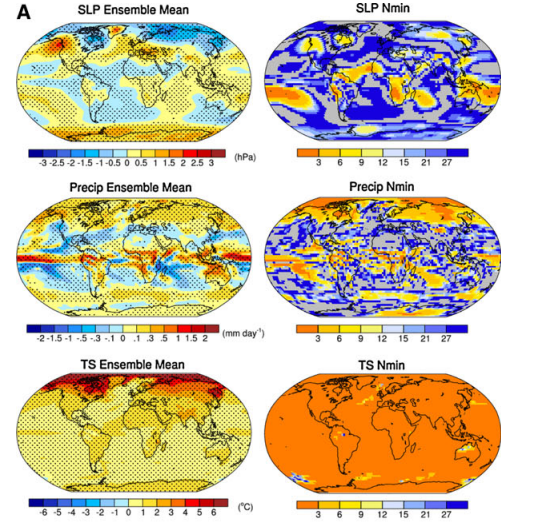
\includegraphics[width=0.8\linewidth]{work/01-variability/figures/EnsembleSenta} 

}

\caption{CCSM3 40-member ensemble (@deser)}\label{fig:EnsembleSenta}
\end{figure}

The climate model ensemble from (\citet{deser}) in more detail. A coupled ocean-atmosphere-land-cryosphere general circulation model (CCSM3) is used. It realistically simulates the main patterns of climate variability, but shows a higher regularity and frequency for ENSO than in nature. The 40-member CCSM3 ensemble uses the T42 version with specific resolutions for the different components and considers the A1B greenhouse gas scenario. The initial conditions for ocean, land and sea ice are identical for each ensemble member and are from 1 January 2000, while the atmospheric conditions vary.
In addition, a 10,000-year control integration of CAM3, the atmospheric component of CCSM3, is used. This integration takes into account recurring seasonal cycles without annual variability based on observations from 1980-2000.
A separate CMIP3 multi-model ensemble was formed for the study, comprising a single integration of 21 models with the SRES-A1B forcing scenario, excluding CCSM3. The climate response was calculated using epoch differences and linear trends for the period 2005-2060. Both methods provide almost identical results. The statistical significance of the results was assessed using a two-tailed Student's t-test.
The left panels of Figure 1a show the ensemble mean epoch difference maps (2051-2060 minus 2005- 2014) for sea level pressure (SLP), precipitation (Precip) and surface temperature (TS) during December-January-February (DJF) for the 40-member CCSM3 ensemble. Hatching indicates areas where the differences are significant at a 95\% confidence level.
After explaining the model and the method, the results are now presented. The ensemble mean response is globally considerable for all three variables. Sea level pressure shows negative values at high latitudes in the northern hemisphere and positive values at mid-latitudes, similarly in the southern hemisphere, but with reversed polarity. These patterns correspond to the northern and southern annular modes (NAM and SAM). The global distribution of SLP changes is consistent with the results of 22 CMIP3 models.
Precipitation shows positive values along the equator and negative values south of it. Subtropics generally have less precipitation, while extratropical regions have more precipitation. The surface temperature is rising everywhere, with stronger warming over land and maximum warming in the Arctic due to the loss of sea ice in autumn.
The right panels of Figure 1a show the minimum number of ensemble members required to detect a significant response. Sea level pressure requires larger ensemble sizes than precip, and surface temperature requires the smallest ensemble sizes. Values for SLP range from less than 6 in the tropics to over 15 in other regions. Precip usually requires fewer members, while TS generally requires less than 3 members, except in some isolated regions. It can also be said that the grey areas indicate the locations where the mean response of the 40-member ensemble is not at the 95\% confidence level.(\citet{deser})

\section{3. Internal variability in the climate system}\label{internal-variability-in-the-climate-system}

The study of internal variability in the climate system is of central importance for understanding the complex interactions and fluctuations within the Earth's climate. Internal variability refers to naturally occurring fluctuations in the climate system that arise independently of external influences such as greenhouse gas emissions, volcanic eruptions or solar variations. This variability can manifest itself on different time scales, from monthly and seasonal fluctuations to decade and century scales.
A prominent example of internal variability is the phenomenon of the North Atlantic Oscillation (NAO), which has a considerable impact on weather and climate conditions in Europe and North America. The NAO influences the temperature and precipitation patterns in these regions through its fluctuations, which in turn can be attributed to the internal dynamics of the circulation systems. The thermohaline circulation also plays a substantial role in internal variability, particularly in the North Atlantic region, where variations in the flow and the associated heat distribution have considerable climatic effects (\citet{latif2022natural}).
The role of internal variability is particularly important for climate research and modelling, as it contributes to considerable uncertainties in climate projections. Models that do not adequately account for this internal variability tend to underestimate or overestimate the variability of the climate system. For example, studies show that the uncertainties in projections of ocean temperatures and ocean currents are influenced by internal variability (\citet{deser}). These uncertainties have a direct impact on the predictability of future climate trends and the planning of adaptation strategies.
The fluctuations in surface temperature and ocean currents observed in the North Atlantic region illustrate the need for precise monitoring and modelling of internal variability processes. This is important in order to distinguish both natural and anthropogenic drivers of climate change and to develop appropriate climate adaptation measures. It is argued that ongoing observation programmes and high model resolutions are necessary to better understand and predict these complex processes (\citet{latif2022natural}).
Internal variability can have both positive and negative effects, depending on the specific climate component and regional characteristics. For example, increased internal variability in the tropics can lead to changes in global atmospheric circulation, which in turn influence climate extremes such as droughts and floods (\citet{deser}).
Understanding these internal processes is therefore crucial for improving the accuracy and reliability of climate models and thus also for developing effective climate change mitigation and adaptation strategies.

\section{3.1 Definition and causes of internal variability}\label{definition-and-causes-of-internal-variability}

Internal variability in the climate system is a central element of climate research and describes fluctuations in the climate that are not caused by external influences such as volcanic eruptions or human activities, but arise from internal dynamics of the climate system itself. The main drivers of this internal variability are the complex interactions between the various components of the climate system, in particular between the atmosphere, oceans, cryosphere and biosphere. Internal variability is the natural variability of the climate system that occurs in the absence of external forcing and includes processes inherent to the atmosphere, ocean and coupled ocean-atmosphere system.
A major cause of internal variability is the thermodynamic coupling between the atmosphere and the near-surface layers of the oceans. This coupling can cause long-lasting climate fluctuations that last for years to decades (\citet{deser}). A prominent example of such variability is the North Atlantic Oscillation (NAO), which is characterised by fluctuations in air pressure between the Icelandic low and the Azores high. These fluctuations have an influence on the weather and climate in the mid-latitudes of the North Atlantic (\citet{latif2009dynamics}).
Another important factor is the wind-driven circulation systems of the oceans, such as the ocean gyre, which can contribute to the Pacific Decadal Oscillation and the Atlantic Multidecadal Oscillation. These processes can be influenced by changes in atmospheric circulation, such as different wind patterns and variations in air pressure (\citet{deser}).
Within the North Atlantic, changes in the thermohaline circulation, also known as the Atlantic Meridional Overturning Circulation (AMOC), play a essential role. This circulation contributes to the distribution of heat within the ocean and is strongly dependent on the salinity and temperature of the seawater. The natural fluctuations of the AMOC can have a considerable impact on the climate of the North Atlantic and lead to multidecadal variations (\citet{latif2022natural}).
The internal variability of the climate system is therefore caused by a variety of mechanisms that operate on different spatial and temporal scales. These mechanisms are often stochastic in nature and can be described by internal dynamical processes such as interactions between ocean and atmospheric wind patterns (\citet{latif2009dynamics}).
In contrast to internal variability, external variability is caused by external drivers; these external factors can influence the climate over longer periods of time. One example of this is changes in solar radiation or volcanic eruptions. In addition, human influences can also play a role, such as greenhouse gas emissons.
To summarise, it can be said that the internal variability in the climate system represents a complex interplay of different factors that include both thermal and dynamic processes. This variability is fundamental to understanding the climate system in all its dynamics and results from the internal interactions of the various climate components. It forms an essential basis for better understanding the uncertainties in climate projections and thus also the planning of adaptation strategies for dealing with climate change.

\section{3.2 Effects of internal variability on climate projections}\label{effects-of-internal-variability-on-climate-projections}

The internal variability in the climate system represents a major uncertainty for climate projections. This variability results from natural processes within the climate system itself and is not caused by external forcing such as greenhouse gases or land-use changes. The internal variability manifests itself on different time scales, from seasonal to multi-decadal, which complicates the interpretation and prediction of future climate conditions.
A key point that illustrates the uncertainties in climate projections is the role of atmospheric circulation. Studies have shown that variations in atmospheric circulation can contribute strongly to uncertainty in climate models (\citet{monerie2020model}). For example, differences in simulated atmospheric dynamics, such as the movement patterns of air masses, contribute essential to the variable amount of precipitation in the Sahel. These uncertainties remain in both older (CMIP5) and newer models (CMIP6) (\citet{monerie2020model}).
Another example of the effects of internal variability is the Atlantic Meridional Overturning Current (AMOC). The AMOC is a large-scale ocean current that transports heat from the tropics to higher latitudes and thus has an influence on regional climate patterns. Studies have shown that the internal variability of the AMOC has been the dominant force since 1900 (\citet{latif2022natural}). Depending on its state, this internal variability can have short-term and long-term effects on the surface temperatures of the North Atlantic and the European climate.
Internal variability is also increased by other factors such as the North Atlantic Oscillation (NAO) and the Atlantic Multidecadal Oscillation (AMO). Fluctuations in these systems can influence the European and North American climate and lead to seasonal to decadal variations in temperature and precipitation (\citet{latif2022natural}).
Furthermore, internal variability complicates policymaking and decision-making as it leads to ranges in climate predictions. This makes accurate predictions difficult and emphasises the need for robust adaptation strategies that consider a variety of scenarios to minimise uncertainties (\citet{tomassini2010uncertainty}).
Finally, it can be stated that internal variability is an important, but often difficult to predict component in climate projections. It strongly influences the uncertainty range of model projections and therefore further studies are urgently needed to better understand the mechanisms of internal variability and to quantify its impact on climate projections more precisely.

\section{4. Application and meaning of climate model ensembles in research}\label{application-and-meaning-of-climate-model-ensembles-in-research}

The use and importance of climate model ensembles in research has grown considerably in recent years. Climate model ensembles are a valuable method for assessing and minimising uncertainties in climate projections. These models make it possible to incorporate the internal variability of the climate system by performing multiple simulations with different initial conditions or model parameters. By using ensemble techniques, the range of possible climate projections can be better understood and the uncertainties arising from internal variability and model specificities can be quantified (\citet{deser}).
However, the role of climate model ensembles goes beyond the mere assessment of uncertainty. They also provide a robust basis for the assessment of climate dynamics under different scenarios and forcing conditions. Ensemble models facilitate the identification of systematic errors in models and enable the assessment of model performance by comparison with observations and other models (\citet{eyring2016overview}). This comparability is particularly important to strengthen confidence in future climate projections and to check the reliability of the models.
In addition, climate model ensembles offer the possibility of analysing the effects of climate change on different spatial and temporal scales. By considering ensembles on a regional scale, researchers can make more accurate predictions about local climate trends and extreme events. This is of particular importance for adaptation to climate change, as it enables decision-makers to develop well-founded and location-specific strategies. For example, modelling can be used to plan agricultural adaptation measures to changing climate conditions by assessing the uncertainties in the projected impacts and using statistical tools such as Monte Carlo simulations (\citet{falloon2014ensembles}).
Another key aspect is the promotion of cooperation within the scientific community. The Coupled Model Intercomparison Project Phase 6 (CMIP6) is an outstanding example that shows how coordinated modelling and data comparison between different research centres help to expand the scientific basis and the validity of climate models (\citet{eyring2016overview}). These collective efforts not only strengthen the quality of the models, but also their ability to respond to the challenges and issues of climate change.
To summarise, climate model ensembles are an indispensable tool in climate research. They help to reduce uncertainty in climate projections, support the development of robust climate predictions and foster deeper collaboration between research centres worldwide. The ongoing development and application of these models will be crucial to better understand the complexities of the climate system and to develop appropriate adaptation strategies.

\section{4.1 Use of climate model ensembles for robust climate predictions}\label{use-of-climate-model-ensembles-for-robust-climate-predictions}

The benefits of climate model ensembles for robust climate predictions are manifold and crucial for the accuracy and reliability of long-term climate projections. These ensembles, which consist of a large number of independent model simulations, make it possible to evaluate and minimise the uncertainties in climate predictions due to internal variability and model-inherent uncertainties.
By using climate model ensembles, the effects of internal variability on future climate projections can be better understood. Internal variability, which is due to natural fluctuations in the climate system, can cause considerable uncertainty in projections (\citet{deser}). Climate model ensembles offer the possibility to quantify these uncertainties by combining a large number of simulations under different initial conditions and with different models. This helps to better map the range of possible future climate states and to increase the robustness of the predictions.
Another advantage of climate model ensembles is the improvement in the statistical representativeness of the climate model outputs. By superimposing many simulations, systematic errors of individual models can be compensated and a more reliable estimate of future climate conditions can be achieved. The probabilistic assessment of future climate trends, as made possible by Bayesian models, ensures that the uncertainties in the model forecasts are adequately taken into account (\citet{smith2009bayesian}).
In addition, climate model ensembles make valuable contributions to the production of regional and seasonal climate predictions, which are of central importance for adaptation strategies at the local level. For example, high-resolution climate models within an ensemble can be used to project specific regional climate changes in more detail (\citet{croce2021enhancing}). This is particularly important for regions that are strongly affected by specific climate extremes, such as the Mediterranean region, where extreme temperature and precipitation events need to be intensively analysed (\citet{croce2021enhancing}).
By considering different emission scenarios in the simulations, the range of possible future climate states can also be covered. This is essential in order to plan and implement adaptive measures that can react flexibly to different climatic developments. A multi-model ensemble thus enables a more robust and comprehensive consideration of climate risks and contributes to improved strategic decision-making (\citet{deser}; \citet{smith2009bayesian}).
To summarise, climate model ensembles provide an indispensable basis for making well-founded and reliable climate predictions. They not only enable a realistic assessment of uncertainties, but also support the development of specialised and regionally adapted climate adaptation strategies. This makes them an essential tool in modern climate research and planning.

\section{4.2 Application examples: regional and seasonal climate trends}\label{application-examples-regional-and-seasonal-climate-trends}

Climate model ensembles play a crucial role in producing robust regional and seasonal climate predictions. By using a multi-model approach, uncertainties can be minimised and the accuracy of projected climate changes can be increased. An illustrative example of this is the study of long-term spatiotemporal variability and trends in extreme rainfall and temperatures in Bangladesh, which can have an impact on rice production (\citet{mainuddin2022long}). The analysis shows regional variations in climate trends, such as the decrease in precipitation in specific regions and the marked rise in temperature, which could substantially affect agricultural yields.
Another example is the use of EURO-CORDEX RCMs and HighResMIP GCMs to analyse the daily precipitation distribution in Europe. These high-resolution models provide an improved representation of precipitation patterns compared to older CMIP5 models. In particular, the PRIMAVERA GCMs show precipitation distributions that are closer to observations in many European regions than the results of the EURO-CORDEX RCMs (\citet{demory2020european}). Such regional climate models are particularly useful for simulating complex topographical and coastal areas more precisely, which is crucial for predicting extreme weather events, for example.
Seasonal trends are of particular interest in climate research as they have a direct impact on agricultural productivity and water resources. Analyses of climate models show that intensified precipitation and longer dry periods have different regional effects. For example, some models show a tendency to overestimate winter rainfall and underestimate summer rainfall, which can be partially corrected by finer grid resolutions (\citet{demory2020european}). Such seasonal discrepancies must be taken into account when planning and adapting agricultural and water management strategies in order to increase resilience to climate change.
The importance of climate model ensembles is emphasised by the combined use of regional and global models. These models make it possible to understand and project the climate at different scales, which is particularly valuable for assessing potential climate risks in specific regions. In this way, the results of this modelling help to develop early warning systems and adaptation strategies that can counter the effects of extreme weather events and support long-term planning (\citet{falloon2014ensembles}). Overall, these application examples illustrate that climate model ensembles are an indispensable tool for analysing and predicting regional and seasonal climate trends. They provide a sound basis for scientifically sound decision-making processes and adaptation planning in the face of advancing climate change.

\section{5. Conclusion}\label{conclusion}

The relationship between natural variability and climate modelling is a central aspect of climate science. Natural variability refers to the natural fluctuations in the climate system caused by internal processes such as El Niño/La Niña, volcanic activity or solar cycles. These fluctuations occur independently of human influences and can affect the climate in the short and medium term. Climate models attempt to take both these natural and anthropogenic (man-made) factors into account in order to provide a realistic simulation of the climate. They use historical data and physical laws to simulate and predict natural climate fluctuations.
Natural variability can cause short-term fluctuations in temperature and precipitation that differ from the long-term trends due to climate change. Climate models show that natural variability can have a major impact on regional climate patterns in the coming decades, even if the long-term trend is dominated by anthropogenic climate change. Scientists compare the results of climate models with historical climate data to assess the accuracy of the models. Models that can correctly simulate natural variability are better able to predict future climate changes.
Despite the progress made in modelling, there are still challenges. The complexity of the climate system and the large number of influencing factors make modelling natural variability a challenge. Moreover, uncertainties regarding future natural events and their impact on the climate system pose an additional difficulty. Overall, natural variability is an integral part of climate modelling, and understanding its mechanisms and influences is crucial for the accuracy of climate projections.

\chapter{Standard Precipitation Evapotranspiration Index}\label{spei}

\emph{Author: Sophie Hopp}

\emph{Supervisor: Henri Funk}

\emph{Suggested degree: Bachelor}

\section{Introduction}\label{introduction-1}

Droughts are a common phenomenon that occurs worldwide and are characterized by prolonged periods of water shortage. These shortages can arise due to various factors such as a lack of precipitation or high temperatures leading to increased evaporation rates. These conditions can arise from natural climate variability and can be worsened by climate change. Droughts can have serious impacts, including agricultural effects such as crop failures and food shortages, disruptions to water supplies, and socio-economic consequences due to restrictions on shipping caused by low water levels (\citet{wilhite1985}). Therefore, it is important to monitor and assess droughts effectively.

Drought indices are used to quantify the severity, duration, and spatial extent of droughts.
There are different types of droughts, such as meteorological, hydrologic, agricultural, and socio-economic droughts (\citet{wilhite1985}). The subjectivity in defining droughts has made it challenging to establish a universal drought index, leading to the development of various indices (\citet{vicente}).

The Standardized Precipitation Index (SPI) is a commonly used index that is based on the probability of precipitation.
It can be calculated for different time scales, which enables to distinguish between short and long-term droughts and is important to functionally separate different drought types. For example, agricultural droughts usually have a much shorter time scale than hydrological droughts (\citet{mckee1993}).
However, the SPI does not take into account the temperature, which can be a critical factor in drought development. It assumes that the variability of precipitation is much higher than that of other variables like temperature and potential evapotranspiration and considers these variables stationary, meaning they have no temporal trend (\citet{vicente}). These assumptions are problematic, especially given the increases in temperature due to climate change, which can have an impact on drought conditions.

The Palmer Drought Severity Index (PDSI), an index primarily used for meteorological droughts, includes temperature by using a soil water balance equation that incorporates prior precipitation, moisture supply, runoff, and surface-level evaporation demand. However, it cannot be calculated for different time scales, has a strong influence of the calibration period, and faces issues with spatial comparability. The self-calibrated Palmer Drought Severity Index (scPDSI) was developed to address some of these issues, but it is still not multiscalar. Since droughts are multiscalar phenomena, they need to be assessed at different time scales (\citet{vicente}, \citet{mckee1993}).

To combine the advantages of both SPI and PDSI, the Standardized Precipitation Evapotranspiration Index (SPEI) was developed. The SPEI is based on the climatic water balance, which is the difference between precipitation and potential evapotranspiration. Like the SPI, the SPEI is based on a probabilistic approach, making the calculation easy and fast. It also shares the multitemporal nature of the SPI, allowing calculation for different time scales (\citet{vicente}).
The inclusion of evapotranspiration in the SPEI allows for a better capture of water deficits or surpluses on the land surface, making it a more effective tool for monitoring and assessing droughts, especially under changing climatic conditions.

This report begins with an introduction to the data, followed by a description of the methods used to calculate the SPEI. The results of the SPEI calculation for Bavaria are then presented, including a comparison of different distributions for the water balance and the proportion of extreme droughts over time.

\section{Data and Methods}\label{data-and-methods}

\subsection{Data}\label{data}

Meteorological data from January 1881 to March 2024 were provided by the Open Data Portal of the Climate Data Center of the German Weather Service (\citet{dwd2024}). The dataset includes regional average monthly observations of the average air temperatures and precipitation in Bavaria. These data were aggregated from grid fields to represent the average conditions for the region.
Bavaria is a federal state in the southeast of Germany with a latitude range of approximately 47° to 50° N and a longitude range of approximately 9° to 13° E.

\subsection{Implementation of the SPEI}\label{implementation-of-the-spei}

To implement the SPEI, we utilized the freely accessible SPEI package (\citet{begueria2023}). This process requires the water balance, for which the potential evapotranspiration must first be determined.

Potential evapotranspiration (\(PET\)) represents the amount of water that would evaporate from the soil and transpire from plants if water supply were not limited. Although various methods exist for calculating \(PET\), it has been shown that their differences have minimal impact on the results of the SPEI (\citet{vicente}). For simplicity, we use the Thornthwaite method to calculate \(PET\). This method relies on the monthly average temperature \(T_i\), the latitude of the study area, and the month of the year. Latitude and time of year are used to estimate solar radiation.

The water balance \(D_i\) is the difference between precipitation \(P_i\) and potential evapotranspiration \(PET_i\) for month \(i\). It is calculated for each month of the year as:

\begin{equation}
D_i = P_i - PET_i, \quad D_i \in \mathbb{R}, i \in \mathbb{Z}.
\end{equation}

Negative values of the water balance indicate a water deficit, while positive values indicate a water surplus.

To calculate the SPEI for different time scales, the water balance is summed over the desired time scale.
The aggregated water balance for a time scale of \(k\) months (\(D^{(k)}_i\)) is calculated as:

\begin{equation}
D^{(k)}_i = D_{i-k+1} + D_{i-k+2} + \ldots + D_i.
\end{equation}

\(D_i^{(k)}\) is later used to compute the SPEI for the respective time scale of \(k\) months, denoted as \(SPEI_i^{(k)}\).

To model the distribution of the aggregated water balance values \(D^{(k)}_i\), a distribution function \(F_D(D_i^{(k)})\) capable of handling negative values and skewed distributions is used.

For the SPI, the gamma distribution is typically employed to model precipitation since precipitation values are strictly non-negative.
However, the gamma distribution is unsuitable for the SPEI because the water balance \(D_i\) can be negative. Instead, the three-parameter log-logistic distribution is used for the SPEI due to its flexibility in modeling skewed distributions, its ability to handle negative values and its relatively high kurtosis, which permits more gradual decrease in the curve for low values.
This results in more coherent and realistic probabilities for very low water balance values, unlike other distributions which suggest that these low values are extremely rare, especially at shorter time scales (\citet{vicente}).

The probability density function of the three-parameter log-logistic distribution is given by:

\begin{equation}
f(x) = \frac{\beta}{\alpha} \left( \frac{x - \gamma}{\alpha} \right)^{\beta - 1} \left( 1 + \left( \frac{x - \gamma}{\alpha} \right)^{\beta} \right)^{-2}, \quad \alpha > 0, \beta > 0, x > \gamma,
\end{equation}

and its cumulative distribution function is defined as:

\begin{equation}
F(x) = \left( 1 + \left( \frac{\alpha}{x - \gamma} \right)^{\beta} \right)^{-1}, \quad \alpha > 0, \beta > 0, x > \gamma,
\end{equation}

where \(\alpha\) is the scale parameter, \(\beta\) is the shape parameter, and \(\gamma\) is the origin parameter that can shift the distribution to model negative values.

These parameters are estimated using the method of L-moments. L-moments are analogous to conventional moments but are less sensitive to outliers, making them a robust and easy approach for parameter estimation (\citet{vicente}).

The distribution for the SPEI is fitted to a reference period, which is typically 30 years. During this period, the climate is assumed to be stationary. The calibration using reference climate data allows for the intercomparison of the index among different stations or periods. Such reference periods are particularly important in climate change studies, as they offer a consistent baseline for assessing temporal changes in drought characteristics (\citet{um2017}).
In this report, the reference period used is from 1981 to 2010. This period serves as a baseline to better understand the extent and severity of droughts in the context of climate variability.

The SPEI values are obtained as the standardized values of \(F_D(D_i^{(k)})\), meaning that the values are centered around zero and have a standard deviation of one. This transformation allows for easy comparison of the SPEI values across different time scales and regions (\citet{vicente}).
One approximation for the SPEI values is given by:

\begin{equation}
SPEI = W - \frac{C_0 + C_1W + C_2W^2 + C_3W^3}{1 + d_1W + d_2W^2 + d_3W^3}
\end{equation}

with

\begin{equation}
W = \begin{cases}
\sqrt{-2\ln(P)} & \text{for } P \le 0.5, \\
-\sqrt{-2\ln(1-P)} & \text{for } P > 0.5
\end{cases}
\end{equation}

and P is the probability that, for a given water balance value \(D^{(k)}_i\), a random value from the fitted log-logistic distribution is greater than the observed value. This probability is calculated as:

\begin{equation}
P = 1 - F_D(D^{(k)}_i).
\end{equation}

The constants are:
\(C_0 = 2.515517, \quad C_1 = 0.802853, \quad C_2 = 0.010328, \quad C_3 = -0.000220,\) \(d_1 = 1.432788, \quad d_2 = 0.189269, \quad d_3 = 0.001308\). \citet{vicente}

\section{Results}\label{results}

\subsection{Comparison of Water Balance Distributions}\label{comparison-of-water-balance-distributions}

To compare the water balance distributions in Bavaria for different time scales, histograms of the water balance values for the commonly used time scales of 1, 3, 6, 12, 18, and 24 months were created for the reference period from 1981 to 2010 (see Figure \ref{fig:modelfittingSPEI}). Both a normal and a log-logistic distribution were fitted to the empirical data. The additional normal distribution is fitted to provide a comparison to the log-logistic distribution. Moreover Figure \ref{fig:modelfittingSPEI} suggests that the normal distribution might be a good fit due to the bell-shaped, symmetric histograms.

For the normal distribution, parameters were estimated using Maximum Likelihood Estimation, which involves using the sample mean and standard deviation to determine \(\mu\) and \(\sigma\).

\begin{figure}
\centering
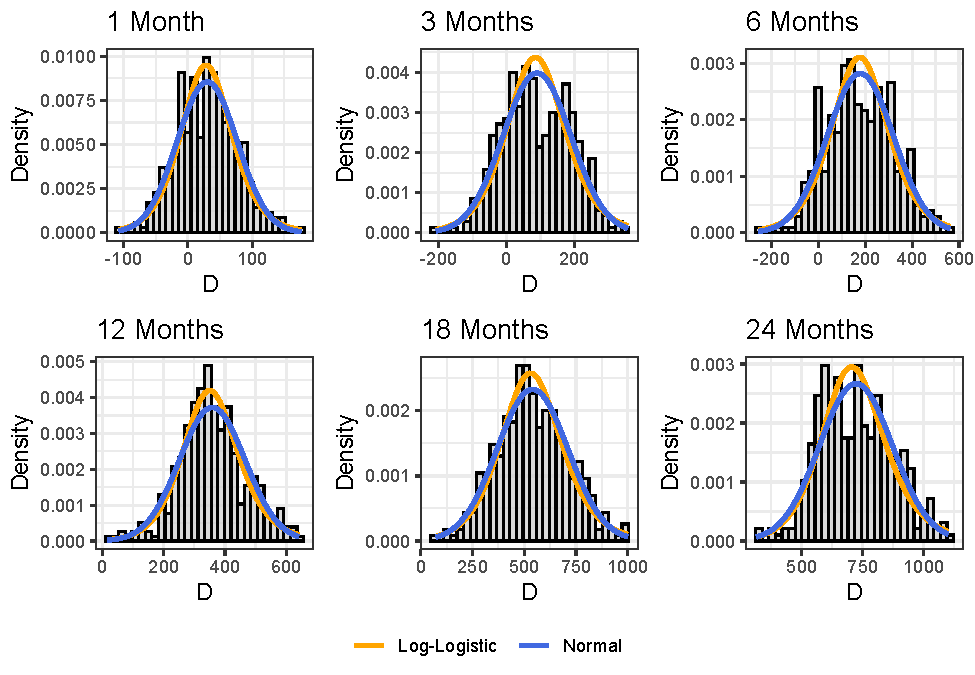
\includegraphics{book_files/figure-latex/modelfittingSPEI-1.pdf}
\caption{\label{fig:modelfittingSPEI}Histograms of the water balance for different time scales (1, 3, 6, 12, 18, and 24 months) with fitted log-logistic and normal distributions for the reference period 1981 - 2010.}
\end{figure}

To compare the goodness of fit of the normal and log-logistic distributions to the empirical water balance data, the Wasserstein distance was calculated.

The Wasserstein distance is a measure of the distance between two probability distributions. The Wasserstein distance is calculated by:

\begin{equation}
\mathcal{W} = \int_{-\infty}^{\infty} |F_{\text{empirical}}(x) - F_{\text{theoretical}}(x)| dx,
\end{equation}

with \(F_{\text{empirical}}(x)\) being the empirical cumulative distribution function and \(F_{\text{theoretical}}(x)\) being the fitted theoretical cumulative distribution function. The smaller the Wasserstein distance, the better the fit of the theoretical distribution to the empirical distribution.

The results of the Wasserstein distance calculation between the empirical distribution and both the fitted log-logistic distribution and the fitted normal distribution for all time scales are shown in Table \ref{tab:wassersteinDistance}.

\begin{table}

\caption{\label{tab:wassersteinDistance}Wasserstein distances between the empirical distribution of the water balance in the reference period from 1981 to 2010 and the fitted normal and log-logistic distributions for different time scales.}
\centering
\begin{tabular}[t]{rrr}
\toprule
Time Scale & Normal & Log-Logistic\\
\midrule
1 & 1.553 & 3.080\\
3 & 7.957 & 12.295\\
6 & 7.511 & 13.667\\
12 & 9.075 & 6.096\\
18 & 6.437 & 11.085\\
\addlinespace
24 & 13.020 & 16.572\\
\bottomrule
\end{tabular}
\end{table}

The Wasserstein distance between the empirical distribution and the fitted normal distribution is smaller than that between the empirical distribution and the fitted log-logistic distribution for all time scales except the 12-month time scale.
This suggests that the normal distribution fits the empirical distribution better than the log-logistic distribution for most of the given time scales in the reference period and the region of Bavaria.
However, the log-logistic distribution with its three parameters offers more flexibility and can model skewness not captured by the normal distribution.
Due to the reasons stated in the methods section, the log-logistic distribution is used for the calculation of the SPEI.

\subsection{SPEI in Bavaria}\label{spei-in-bavaria}

\begin{figure}
\centering
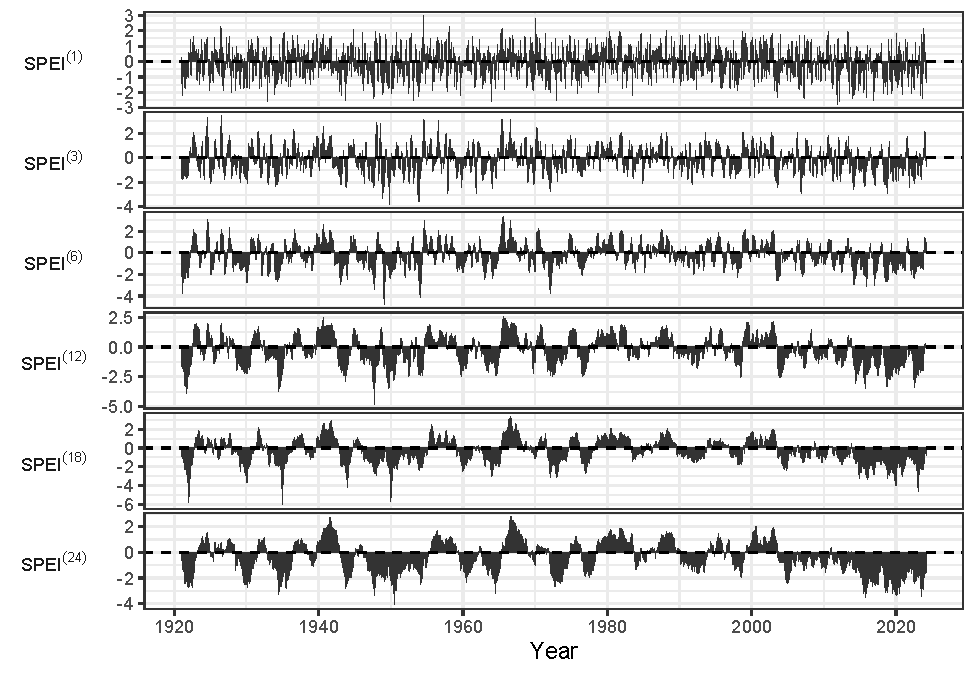
\includegraphics{book_files/figure-latex/spei-1.pdf}
\caption{\label{fig:spei}The 1-, 3-, 6-, 12-, 18-, and 24-month SPEI for Bavaria (1921 - 2024).}
\end{figure}

The SPEI for Bavaria for different time scales is shown in Figure \ref{fig:spei}.
Values below 0 indicate that there is less water available than usual, while values above 0 indicate that water availability is higher than on average.
All subplots show fluctuations around the zero line, indicating periods of both wet and dry conditions. Longer aggregation periods show smoother patterns compared to shorter periods.
The 1-month SPEI shows the highest variability due to its sensitivity to short-term fluctuations in precipitation and temperature.
There is a trend toward more negative SPEI values in the last years, indicating a decrease in water availability and increasing drought conditions. This trend is mostly visible in the longer time scales.
Historically, Bavaria has experienced extended periods with both negative and positive SPEI values, but in recent years, there have been no prolonged periods with positive SPEI values visible in the 12-, 18-, and 24-month SPEI.

\begin{table}

\caption{\label{tab:speiClassification}Classification of Droughts Based on the SPEI (@mckee1993).}
\centering
\begin{tabular}[t]{ll}
\toprule
SPEI & Classification\\
\midrule
0 to -0.99 & Mild Drought\\
-1 to -1.49 & Moderate Drought\\
-1.5 to -1.99 & Severe Drought\\
\$\textbackslash{}leq -2\$ & Extreme Drought\\
\bottomrule
\end{tabular}
\end{table}

Table \ref{tab:speiClassification} shows the classification of droughts based on the SPEI. These drought categories were originally defined for the SPI but are commonly used for the SPEI due to the standardized nature of the indices.
An index below -2 indicates extreme drought (\citet{mckee1993}).

To visualize the frequency of extreme droughts in Bavaria over time, the proportion of months experiencing extreme drought within a given period is calculated using the following formula:

\begin{equation}
prop_{i,m}^{(k)} = \frac{\sum_{j=i-m+1}^{i} \text{I}(SPEI_{j}^{(k)} \leq -2)}{m}
\end{equation}

where \(prop_{i,m}^{(k)}\) represents the proportion of months experiencing extreme drought for a specific SPEI scale \(k\) within the period ending at month \(i\) and covering the last \(m\) months. \(\text{I}\) is an indicator function that equals 1 if the SPEI value is less than or equal -2 and 0 otherwise.

\begin{figure}
\centering
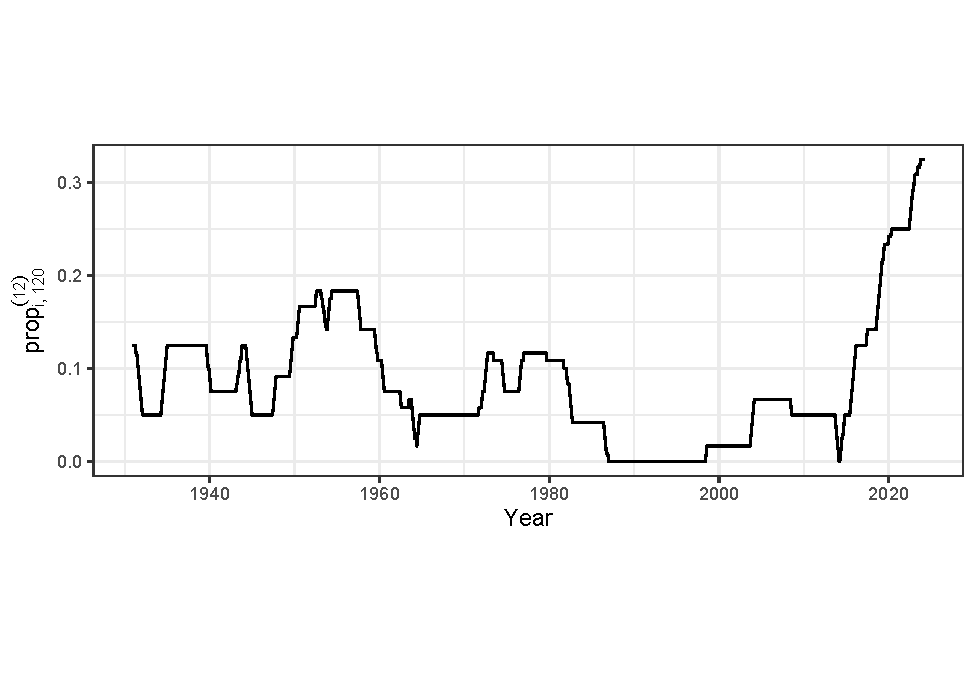
\includegraphics{book_files/figure-latex/extremeDroughts-1.pdf}
\caption{\label{fig:extremeDroughts}Proportion of 12-month SPEI values below -2 for periods of 10 years in Bavaria (1921 - 2024).}
\end{figure}

Figure \ref{fig:extremeDroughts} displays the proportion of 12-month SPEI values below -2 over consecutive 10-year periods. Historically, Bavaria has experienced periods of extreme drought, however the proportion of months classified under extreme drought conditions has continuously increased over the past decade. Currently, this proportion is at its highest level in the past century, with 32.5\% of the months in the last 10 years recording an \(SPEI^{(12)}\) value below -2.

\begin{figure}
\centering
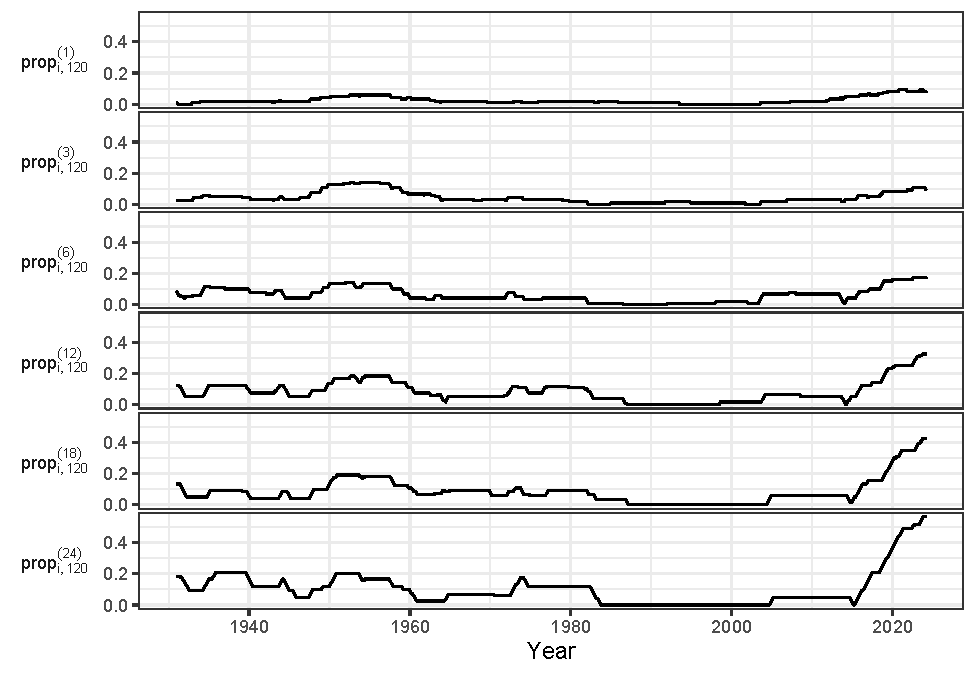
\includegraphics{book_files/figure-latex/extremeDroughts2-1.pdf}
\caption{\label{fig:extremeDroughts2}The proportion of extreme droughts in Bavaria in the last 10 years for different time scales of the SPEI (1, 3, 6, 12, 18, and 24 months).}
\end{figure}

When comparing the proportion of extreme droughts using different time scales for the SPEI, it is evident that the proportion of extreme droughts has increased across all time scales in recent years (see Figure \ref{fig:extremeDroughts2}). The data shows that the longer the time scale, the higher the proportion of extreme droughts.
For the 24-month SPEI, the proportion of extreme droughts is at the moment above 50\%.
However, for the 3-month SPEI, the proportion of extreme droughts is not at its highest level in the last 100 years. Notably, from approximately 1952 to 1956, the proportion of extreme droughts was higher than in recent years when considering the 3-month SPEI. This mid-20th century period of increased drought conditions is also apparent across other time scales, but the proportion of extreme droughts in recent years surpasses that of the 1950s.

\begin{figure}
\centering
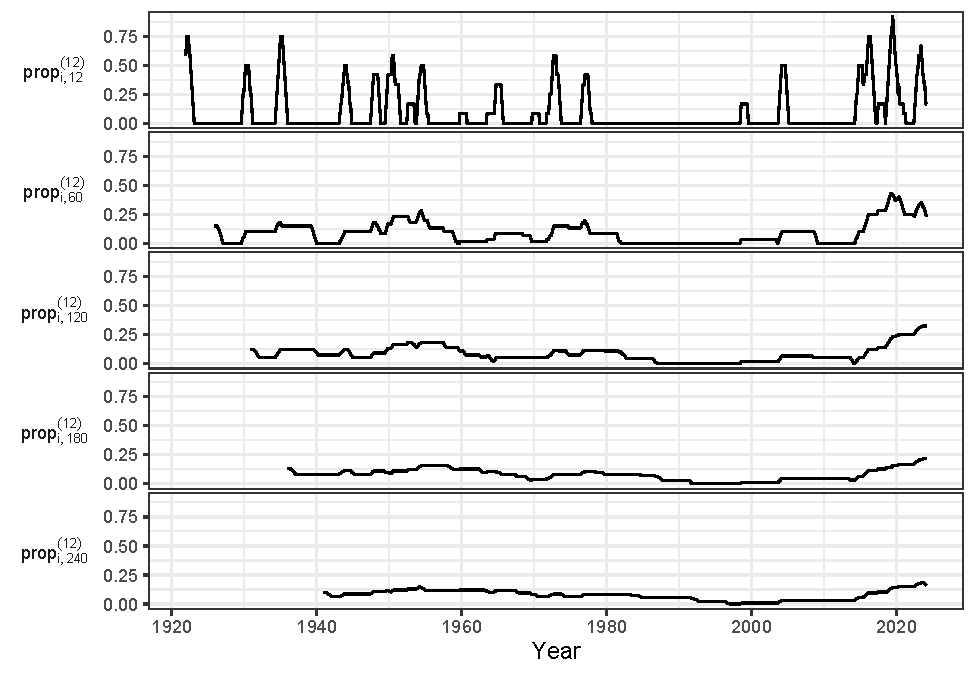
\includegraphics{book_files/figure-latex/extremeDroughts3-1.pdf}
\caption{\label{fig:extremeDroughts3}The proportion of extreme droughts in Bavaria by SPEI12 for different periods of the SPEI (1, 5, 10, 15, and 20 years).}
\end{figure}

When using different periods for the calculation of the proportion of extreme droughts, the data reveals that the proportion of extreme droughts has a higher variability for shorter periods (see Figure \ref{fig:extremeDroughts3}).

\section{Discussion}\label{discussion}

The results demonstrate that the SPEI is a valuable and practical tool for monitoring drought conditions over different time periods. By considering both precipitation and potential evapotranspiration, the SPEI provides a comprehensive measure of water availability and accounts for climatic factors that affect the water balance beyond what precipitation-based indices, such as the SPI can offer. This sensitivity to climate change allows the SPEI to effectively identify the impacts of global warming on drought conditions.

The SPEI's minimal data requirements, ease of calculation, and multiscalar nature contribute to its wide applicability. Additionally, it is robust across different climatic regions due to the log-logistic distribution used in its calculation.

However, a limitation of the SPEI is its dependence on the accuracy of potential evapotranspiration estimates, which can vary depending on the calculation method. For instance, the Thornthwaite method used in this report assumes that evapotranspiration does not occur when the temperature is below 0°C. This assumption might not be accurate in regions where evapotranspiration can still occur at low temperatures due to factors like wind speed and solar radiation. While other methods can provide more accurate PET estimates, they require additional data that may not be available in all regions.

The Global Precipitation Climatology Centre Drought Index (GPCC-DI) combines the SPEI with an adapted version of the SPI to account for the limitations of both indices. The SPEI works well in warm, dry regions where the SPI is not applicable, while the SPI is effective in cold regions where estimating potential evapotranspiration is challenging. This combination allows for almost global coverage (\citet{ziese2014}).

An important consideration in using the SPEI is the choice of the reference period, as it influences the assessment of drought characteristics, particularly the severity and spatial extent, while its impact on frequency is relatively small. It is recommended that the reference period be clearly specified in drought assessments to improve understanding of regional drought characteristics and their temporal changes (\citet{um2017}).

The observed trends in Bavaria indicate an increase in the frequency of extreme drought conditions, particularly in the last decade. These trends are especially pronounced at longer time scales.

One application of the SPEI is predicting future drought conditions. Accurate predictions can enable better preparedness and mitigation strategies, thereby reducing the negative impacts of droughts. \citet{mathivha2020} investigated the use of generalized additive models to predict the SPEI, incorporating variables such as rain, minimum, maximum and average monthly temperature as predictors in addition to lagged SPEI values.
Using observations such as temperature and precipitation, that can only be measured retrospectively to predict drought conditions of already passed months is not useful as they are not future predictions anymore. However, the use of lagged SPEI values can be a valuable tool for drought prediction.
It would be beneficial to investigate the use of other models to predict future drought conditions based on lagged SPEI values.

\chapter{Compound events}\label{ce}

\emph{Author: Shiyu Lu}

\emph{Supervisor: Henri Funk}

\emph{Suggested degree: Master}

\section{Abstract}\label{abstract-1}

As global temperatures continue to warm, extreme weather is occurring more frequently. In climate research, a combination of multiple extreme weather or climate events occurring simultaneously or sequentially is known as a compound event. This can cause more severe impacts than one extreme weather alone. Hot and dry is often considered as one such compound event. In this paper, we take Germany and the Bundesland as an example, and analyze temperature and precipitation data from 1881 to 2023 by fitting a Copula model to study the occurrence of a composite event: hot and dry.

\section{Introduction}\label{introduction-2}

With global warming, extreme weather is becoming more frequent, in 2023, the \citet{wmo2023a} had released a news that stated extreme weather will become the ``new norm''. And in the year 2024 immediately afterward, \citet{wmo2024} released news again and mentioned more extreme heat. In other words, the occurrence of extreme weather is still tending to become more and more common today. The effects of extreme heat have been widely discussed and researched, but there are more different types of extreme weather and the terrible thing is that they don't always happen alone.

In climate research, a compound event is a combination of multiple extreme weather or climate events that occur simultaneously or sequentially. And the previously mentioned hot is often considered with the dry together to be as such compound events. This means that the interactions between hot and dry amplify the consequences, which are more severe than the impacts that would be expected if these events occurred separately. Extremely dry and hot weather poses a great risk to many fields, such as agriculture (\citet{lesk2016}), ecology (\citet{jentsch2008}) and human health (\citet{libonati2022}) etc. Therefore, it is important to study the frequency of compound events of hot and dry and to predict the probability of extreme hot and extreme dry climates in the future.

In this study, Germany is used as examples, temperature and precipitation data from beyond 1881 will be studied to analyze and predict the occurrence of extreme hot and extreme dry weather. \citet{zscheischler2020} have used Copula models to analyze and study temperature and precipitation in Germany up until 2019, as the compound hot and dry in 2018 German growing season had broken records. And in this study, we refer to some of the research methods used in that study and update the data to 2023, which is the latest and most complete data that can be collected now, in order to follow the changes in the data. At the same time, in addition to the study for Germany as a whole, we also focus on the Bundesland in order to make the data more varied, so that we can observe and compare the differences in hot and dry compounds between the Bundesland states.

During the study we start by finding the most suitable Copula model for each data i.e.~for different regions, this process can be achieved by using the function ``BiCopSelect()'' in the R package VineCopula (\citet{schepsmeier2018}). After that we plot contour lines for the data based on the model and also plot a scatter plot to help observe the distribution of data points. In addition, in order to observe the occurrence of extreme heat and dryness composite events, we follow the approach from \citet{zscheischler2020}, that is to introduce four intuitive hazard scenarios, define the criteria for extreme hot and dry by using the 2018 data as the threshold and similarly presented them in the graphs. At the end we also perform simulations based on the model so that we can predict the probability of extreme hot and dry weather to occur in the future in Germany and its Bundesland.

There are three main data sets that will be used in this study, which are temperature and precipitation average over Germany as provided by the \citet{dwd2024b} and observation-based estimates of annual global mean temperature anomalies from the \citet{giss2024}, they are all from 1881 to 2023. It is worth noting that for temperature and precipitation data we only focus on the growing season, March to November, and the summer season, June to August, which prevents possible extreme cold winter weather from weakening possible hot weather when calculating temperature averages. In addition the analysis of the growing season has shown great meaning for agriculture.

\section{Theoretical Background}\label{theoretical-background}

\subsection{Copula}\label{copula}

Copulas are multivariate distribution functions whose one-dimensional margins are uniform on the interval \([0,1]\) (\citet{nelsen2006}) and used to describe the dependence between random variables. \citet{salvadori2016} introduced Copulas using the following notation. In fact Copula can be multivariate, but since this article studies hot and dry, we focus on the bivariate Copula. Let \(C\) denote a bivariate Copula and \(F\) a bivariate cumulative distribution function, by Sklar's Theorem, we have:

\[F(x) = P(X_1 \leq x_1, X_2 \leq x_2) = C(F_{1}(x_1), F_{2}(x_2)) \tag{1} \]
for all \(x \in R^2\), where \(F_1\) and \(F_2\) are the univariate margins of \(F\) (\citet{sklar1959}).

The formula of probability distribution function \(f\) is:

\[f(x) = f_1(x_1) f_2(x_2) c(u_1, u_2) \tag{2} \]

and \(c\) here represents the copula density.

The (joint) survival function can be denoted as:

\[\bar{F}(x) = P(X_1 > x_1, X_2 > x_2) = \hat{C}( \bar{F}_1(x_1), \bar{F}_2(x_2)) \tag{3} \]

where \(\hat{C}\) represents the survival copula of the \(X_i\)'s and \(\bar{F}_i\) represents the survival function of \(X_i\), \(i = 1, 2\).

The Kendall's function \(K\) associated with the copula \(C\) of \(X\) can be written as:

\[K(t) = P\left(F(X_1, X_2) \leq t\right) = P\left(C\left(F_1(x_1), F_2(x_2)\right) \leq t\right) \tag{4} \]

with \(t \in [0,1]\) and the upper-orthant Kendall distribution function \(\hat{K}\) can be stated as:

\[\hat{K}(t) = P\left(\bar{F}(X_1, X_2) \leq t\right) = P\left(\hat{C}\left(\bar{F}_1(x_1), \bar{F}_2(x_2)\right) \leq t\right) \tag{5} \]

These formulas are not only important for the copula, but also very useful when defining four intuitive hazard scenarios afterwards.

Kendall's Tau is a correlation coefficient, for copula we can calculate it to describe the direction and strength of the relationship between two variables. Kendall's Tau can be computed as follows (\citet{barbe1996b}):

\[\tau = 4E(C(U, V)) - 1= 4 \int_{0}^{1} t \, dK(t) - 1 \tag{6} \]

Kendall's Tau takes values between -1 and 1, with 1 representing Perfect positive dependence, -1 representing Perfect negative dependence and 0 representing independence.

Upper Tail Dependence (UTD) refers to the dependence which is shown when both variables reach their upper values, it is a better representation of the dependence between extreme values. We can calculate UTD using the following formula (\citet{fischer2006}):

\[\lambda_U \equiv \lim_{{u \to 1^-}} P(Y > F_Y^{-1}(u) \mid X > F_X^{-1}(u))= \lim_{u \to 1^{-}} \frac{1 - 2u + C(u, u)}{1 - u} \tag{7} \]

UTD ranges from 0 to 1, with 1 representing Perfekt Upper Tail Dependence, i.e.~when one variable reaches its maximum value, the other variable also reaches its maximum value. Whereas 0 represents no Upper Tail Dependence.

\subsection{Empirical Copula}\label{empirical-copula}

Empirical Copula does not need to assume marginal distributions, but still captures the dependency structure between variables in the dataset. The specific function can be written as (\citet{bucher2013}):

\[C^n(u_1, u_2) = \frac{1}{n} \sum_{i=1}^n \mathbb{I}\left(U_{i1} \leq u_1, U_{i2} \leq u_2\right) \tag{8} \]

where \(U\) stand for constructing pseudo-copula observations using the empirical distribution function.

\subsection{Archimedean Copulas}\label{archimedean-copulas}

Archimedean Copulas defines a family of copulas that often have an explicit formula and satisfy the following conditions (\citet{mcneil2009}):

\[C(u_{1}, u_{2}; \theta) = \psi^{-1}\left( \psi(u_{1}; \theta) + \psi(u_{2}; \theta); \theta \right) \tag{9}\]

where \(\psi : [0,1] \times \Theta \rightarrow [0,\infty)\) is called generator function. And \(\psi^{-1}\) is defined as its pseudo-inverse:

\[\psi^{-1}(t; \theta) =
\begin{cases}
    \psi^{-1}(t; \theta) & \text{if } 0 \le t \le \psi(0; \theta) \\
    0 & \text{if } \psi(0; \theta) \le t \le \infty
\end{cases} \tag{10}\]

Note that there are many other families of Copulas, but the two Copula models that were used the most in this study are from this family.

Joe Copula belongs to Archimedean copulas and has a good ability to capture the Upper Tail Dependency, Joe Copula and its generator function can be represented like the following (\citet{triantafyllou2024}):

\[\phi(t) = -\log\left(1 - (1 - t)^\theta\right), \ \ \theta \geq 1 \tag{11}\]
\[\phi^{-1}(t) = 1 - ((1 - e^{-t}))^{1/\theta}, \ \ \theta \geq 1 \tag{12}\]
\[C(u_1, u_2; \theta) = 1 - \left[ (1 - u_1)^\theta+(1 - u_2)^\theta - (1 - u_1)^\theta(1 - u_2)^\theta)\right]^{1/\theta} \tag{13}\]

Clayton Copula also belongs to the Archimedean copulas, but it is better at capturing Lower Tail Dependencies. Clayton Copula and its generator function are represented as follows (\citet{chesneau2023}):

\[\phi(t) = \frac{1}{\theta} (t^{-\theta} - 1), \ \ \theta \in [-1, \infty) \backslash \{0\} \tag{14}\]
\[\phi^{-1}(t) = (1 + \theta t)^{-\frac{1}{\theta}}, \ \ \theta \in [-1, \infty) \backslash \{0\} \tag{15}\]
\[C(u_1, u_2; \theta) = \left[\max\{u_1^{-\theta} + u_2^{-\theta} -1;0\}\right]^{-\frac{1}{\theta}} \tag{16}\]

Since in this study we focus on the Upper Tail Dependence, we do not use the Clayton Copula directly, but we can obtain the Survival Clayton Copula, also known as the rotated Clayton Copula, by rotating the Clayton Copula.

\subsection{Intuitive Hazard Scenarios}\label{intuitive-hazard-scenarios}

AND Scenario:

\[ \text{P}_\text{AND} = P(U > u \cap V > v) = 1 - u - v - C(u, v) \tag{17}\]

OR Scenario:

\[ \text{P}_\text{OR} = P(U > u  \cup V > v) = 1 - C(u, v) \tag{18}\]

Kendall Scenario:

\[ \text{P}_\text{K} = P(C(U, V) > t) = 1 - K(t) \tag{19}\]

Survival Kendall Scenario:

\[ \text{P}_\text{SK} = P( \hat{C}(1 - U, 1 - V) < t) = \hat{K}(t) \tag{20}\]

Of the four Intuitive Hazard Scenarios cited, \(\text{P}_\text{AND}\) and \(\text{P}_\text{OR}\) are very easy to understand, Pand considers both variables to be large, while Por considers that only one of the variables needs to be large. The \(\text{P}_\text{K}\) and \(\text{P}_\text{SK}\) can be characterized by the ``critical layers'' \(L_t\) and \(\bar{L}_t\), respectively, which separates the bivariate space into a critical region and a non-critical region (\citet{zscheischler2020}).

\section{Descriptive Analysis}\label{descriptive-analysis}

\subsection{Climate Map of Germany}\label{climate-map-of-germany}

\begin{figure}

{\centering 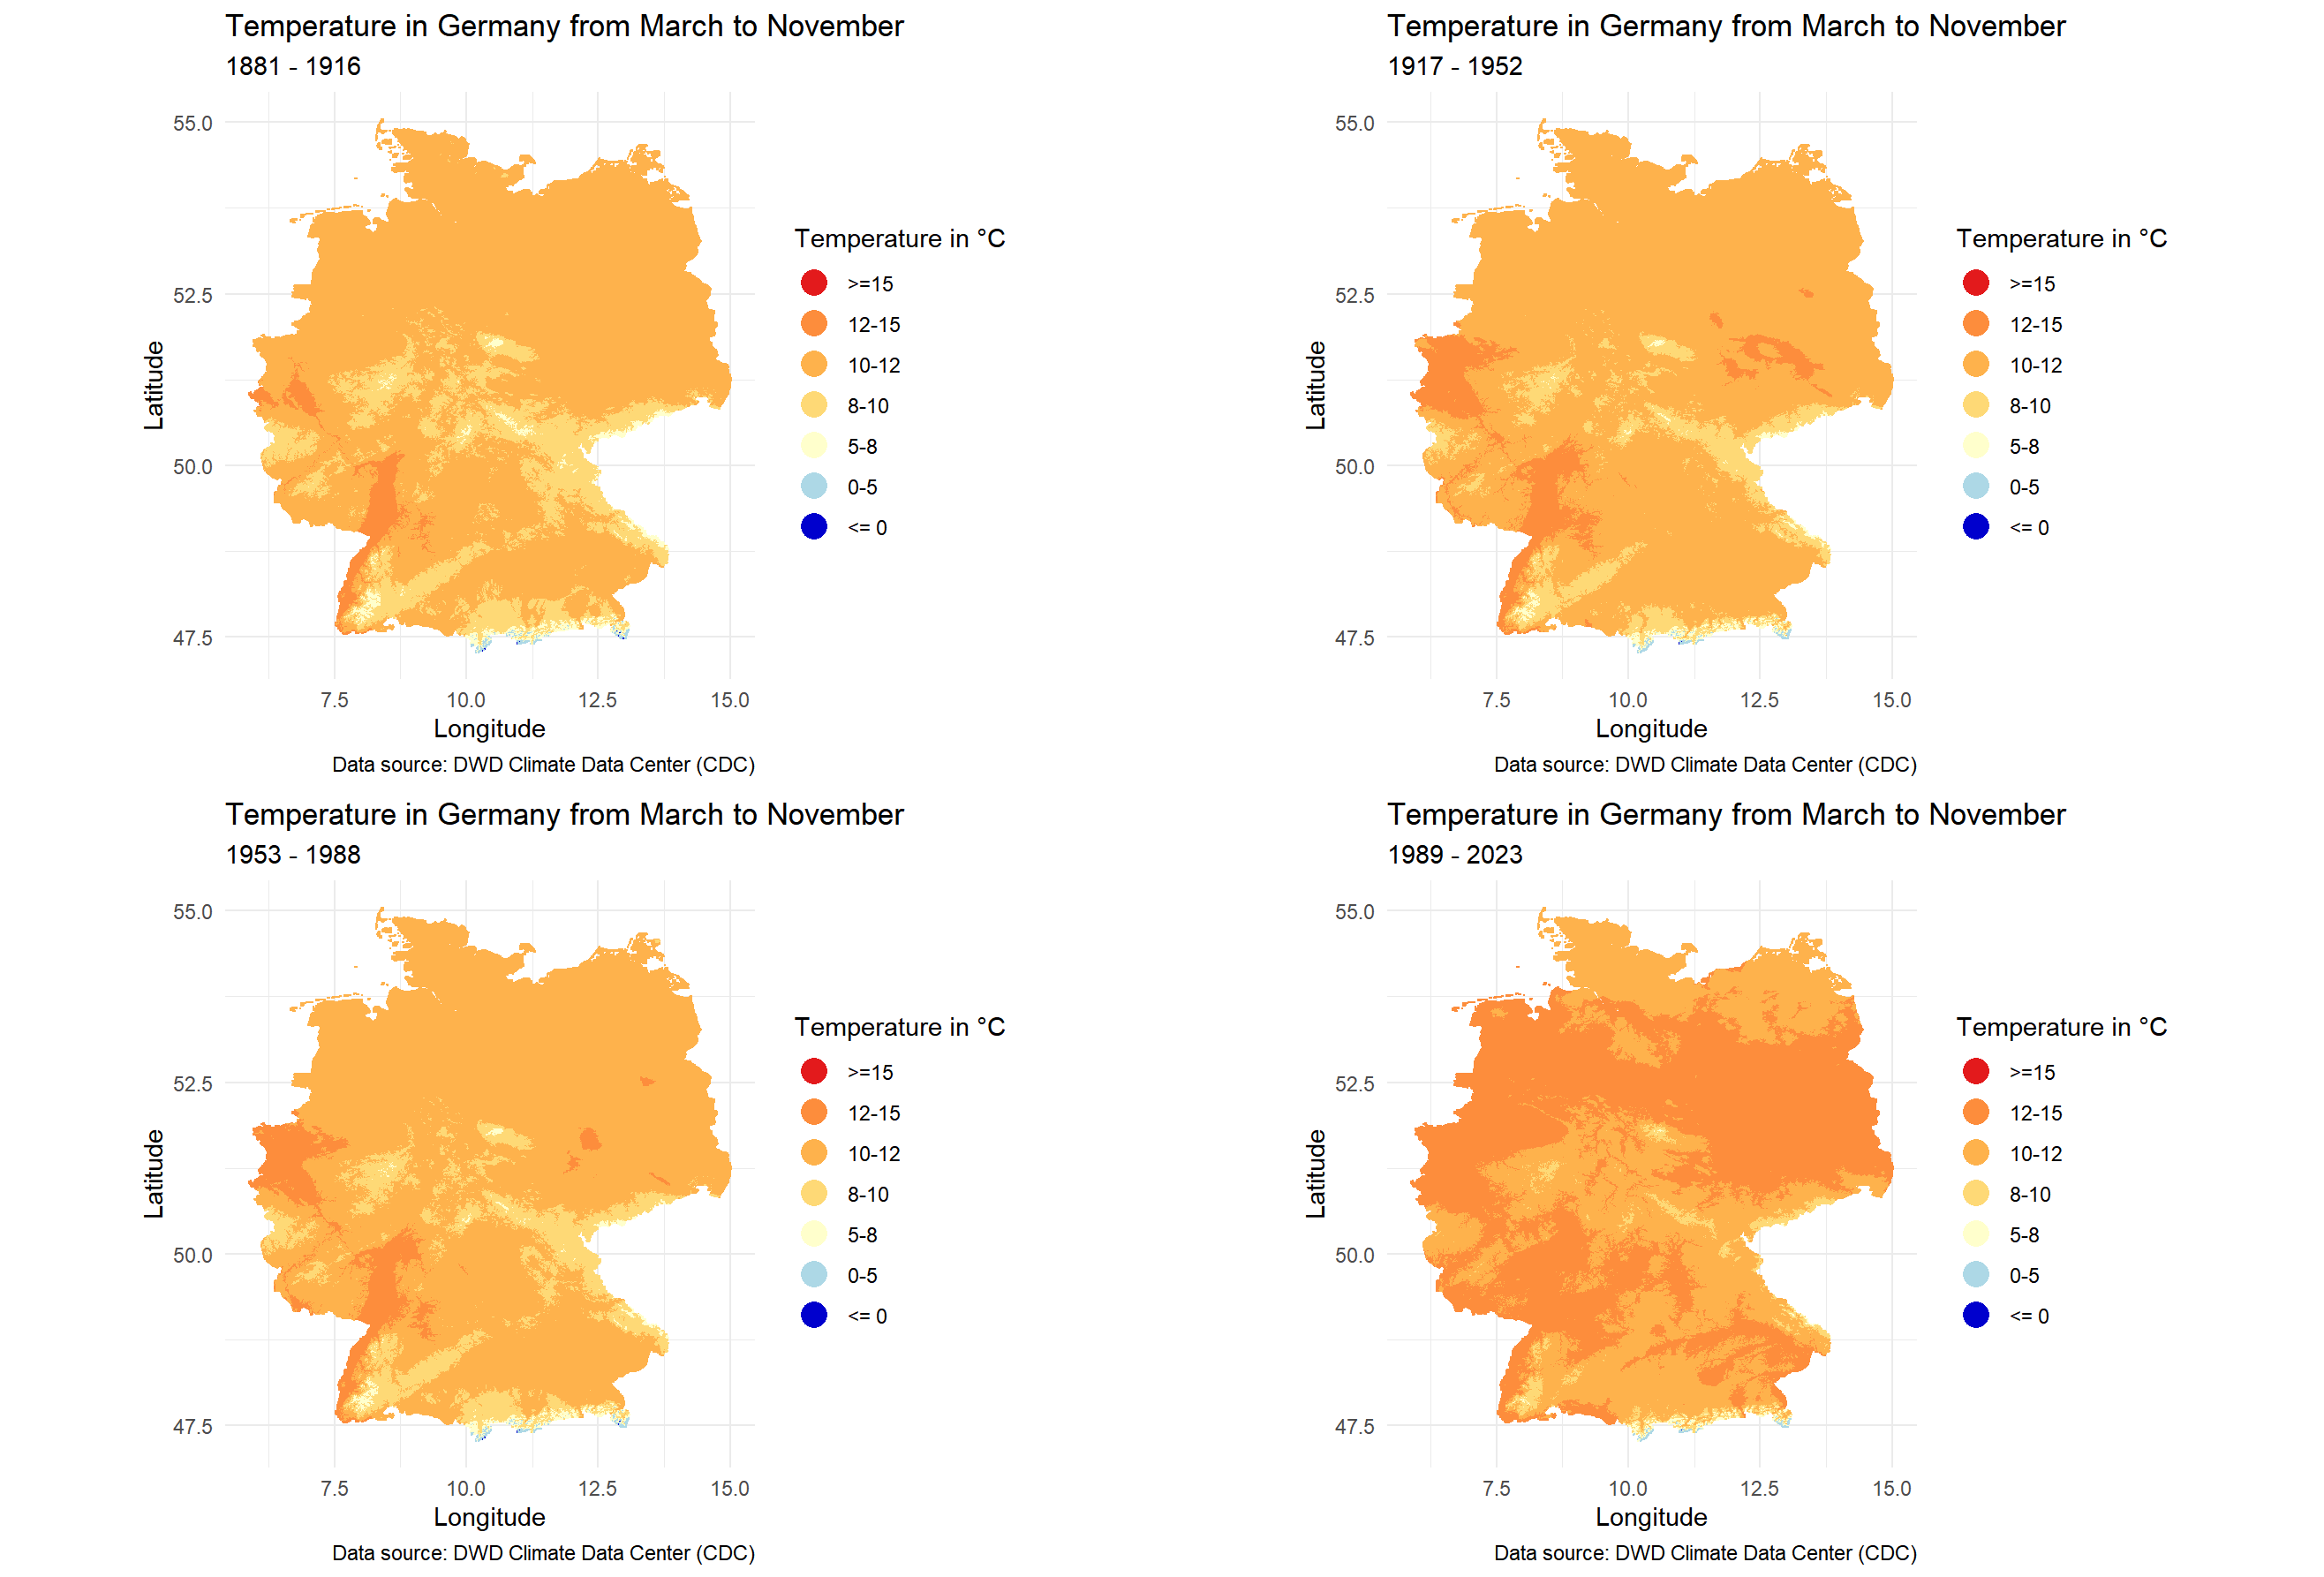
\includegraphics[width=0.8\linewidth]{work/03-compounds/figures/Temperature/Temperature} 

}

\caption{Temperature map in Germany from March to November}\label{fig:climatemap3-shiyu}
\end{figure}

\begin{figure}

{\centering 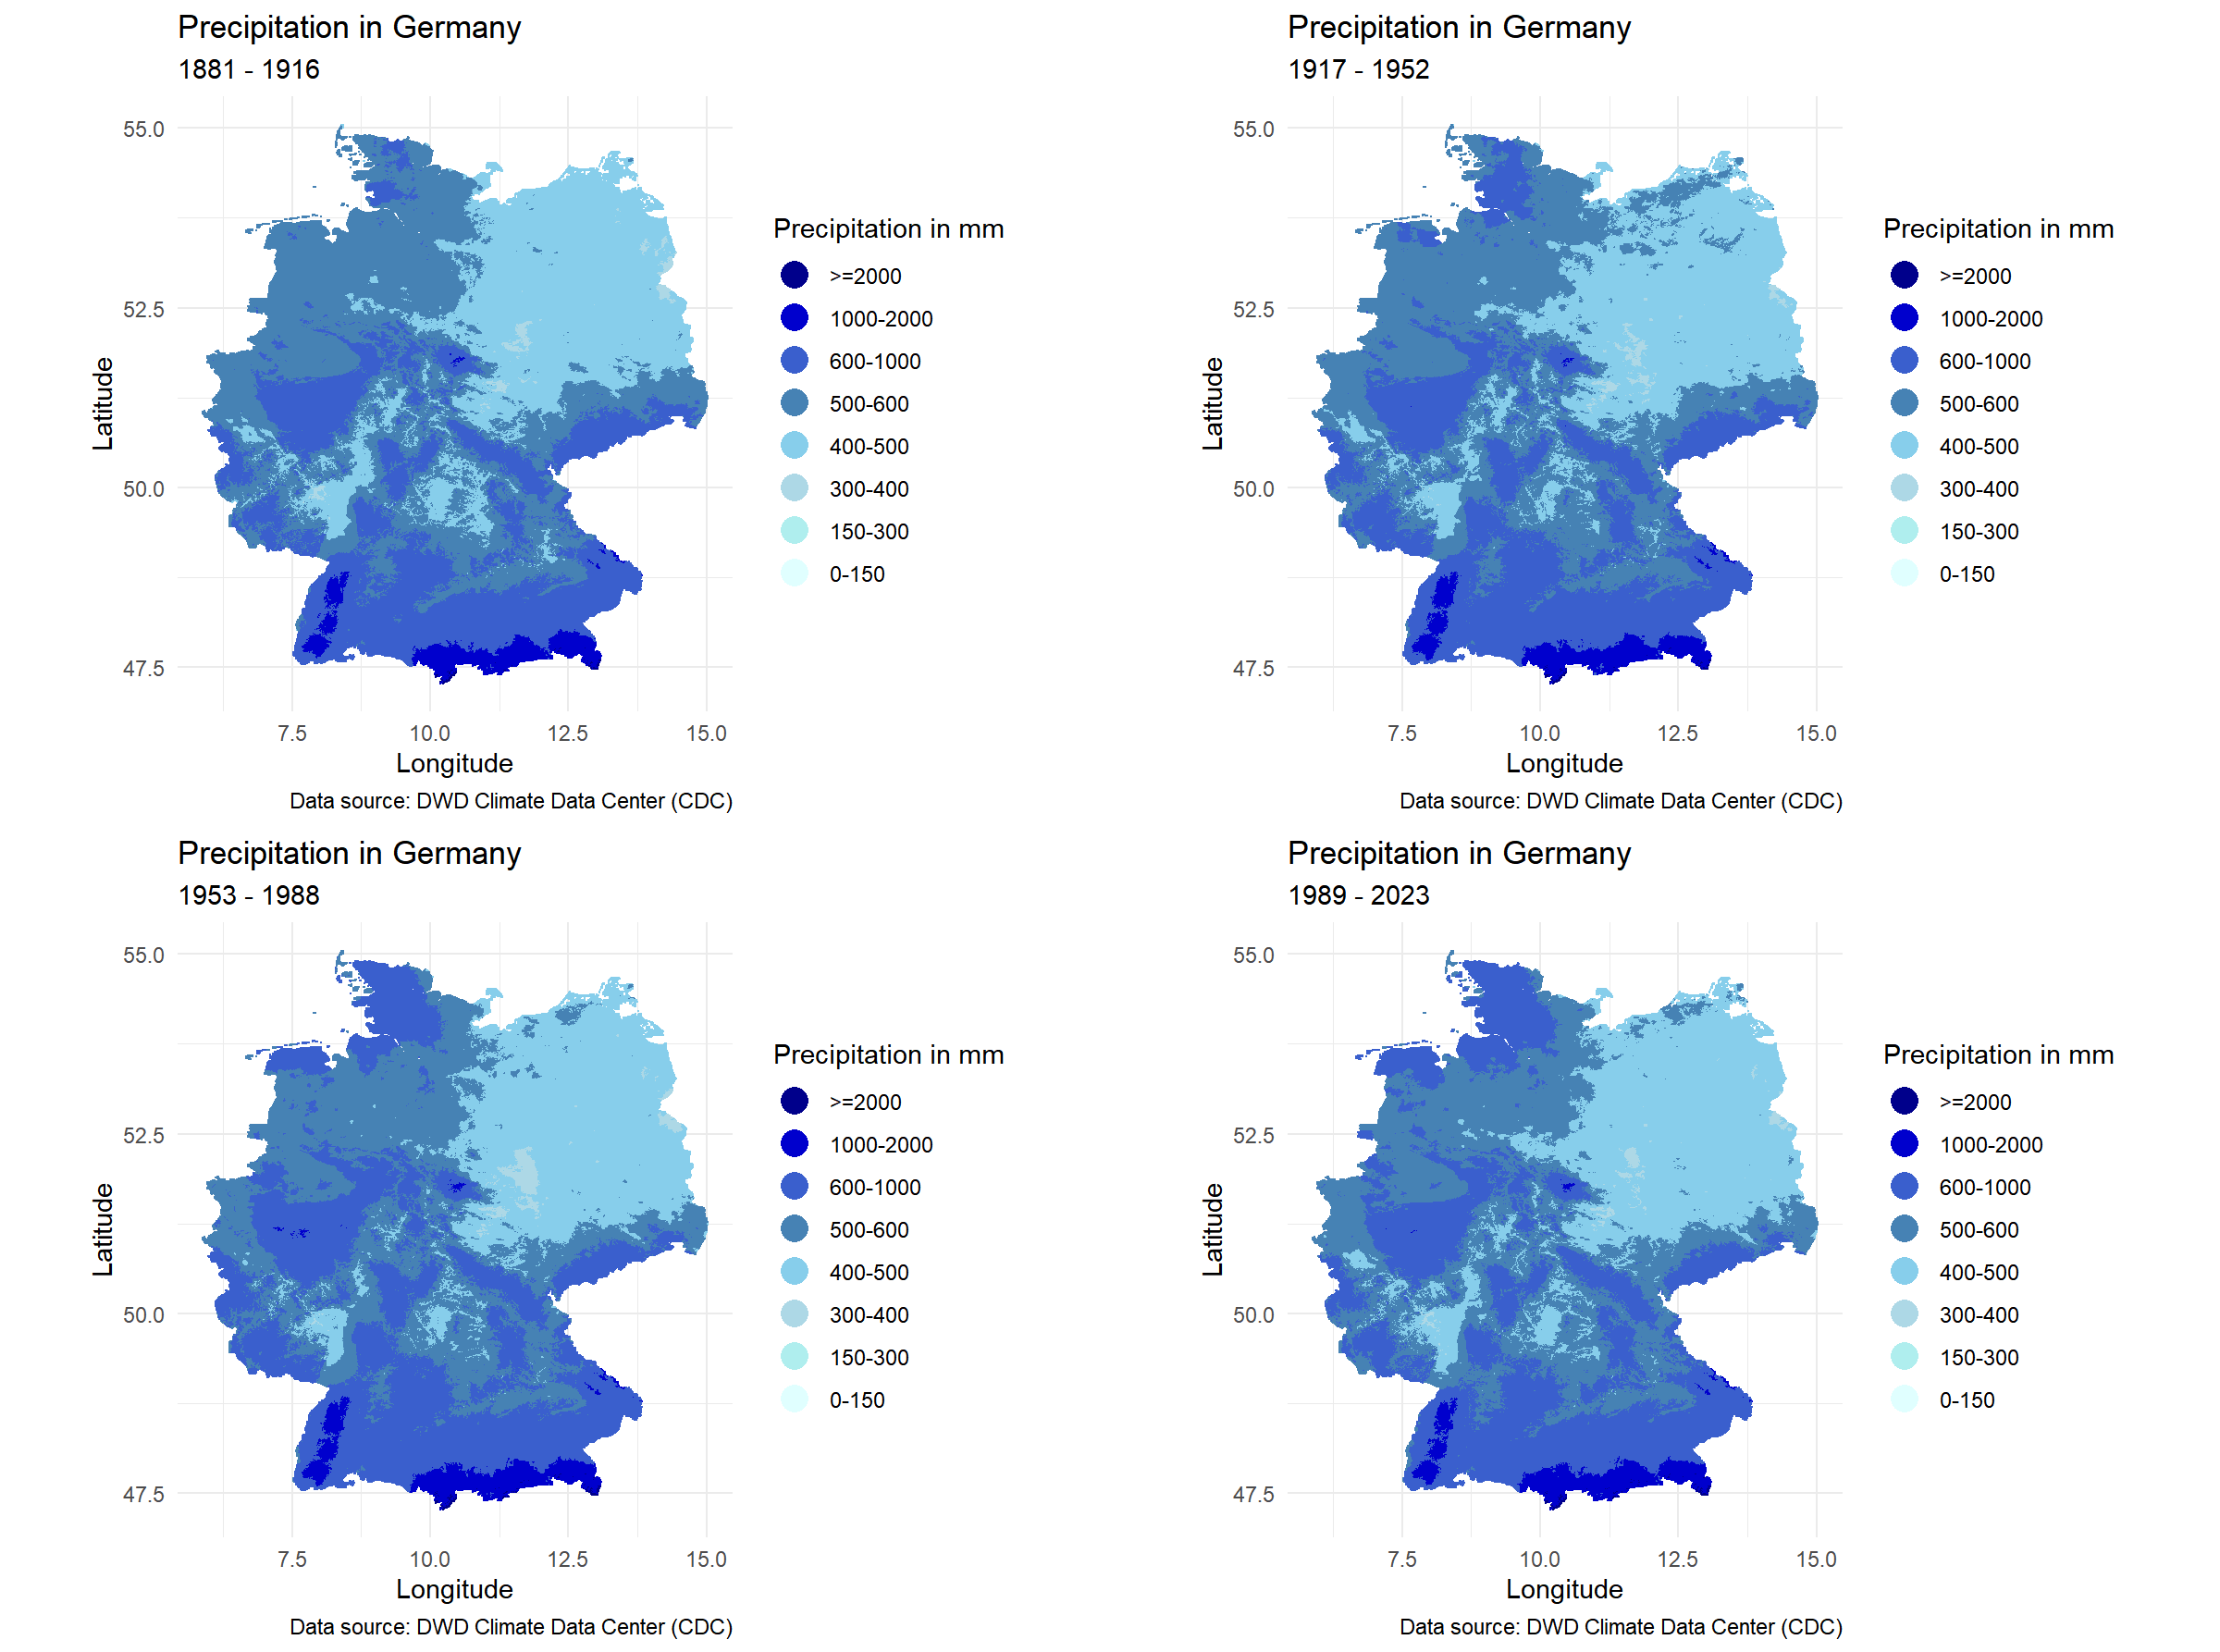
\includegraphics[width=0.8\linewidth]{work/03-compounds/figures/Precipitation/Precipitation} 

}

\caption{Precipitation map in Germany from March to November}\label{fig:climatemap4-shiyu}
\end{figure}

In climate maps we can see two climate maps of Germany from 1881 to 2023, showing the changes in temperature as well as precipitation from March to November over the years, from which we can already see that there is a clear upward trend in temperature, which clearly echoes global warming. By focusing on the regional characteristics we can also see that the south-west corner of the country is the place with the lowest temperatures and also the most precipitation, while the north-east, Sachsen-Anhalt, Brandenburg and Berlin have relatively the highest temperatures and the least amount of precipitation in Germany, this characteristic matching exactly the compound event hot and dry that we want to study.

The situation for June to August is very similar.

\subsection{Development of Average Data in Germany as a whole}\label{development-of-average-data-in-germany-as-a-whole}

Dynamic maps allow us to view trends in data from all corners of Germany, and after comparing differences by region, we can look at temperature and precipitation changes over the 143 years as a whole. We can more visually feel in Figure \ref{fig:AverageTemperature-shiyu} that there is a very clear upward trend in temperatures, both from March to November and from June to August, and that the average summer temperatures will be significantly higher than those from March to November, and we can also focus on the fact that 2018, which is the location, does have super high temperatures, it has the highest temperatures in the March to November comparison, and it comes second in June to August, but the difference with the hottest year is not too great either.

\begin{figure}

{\centering 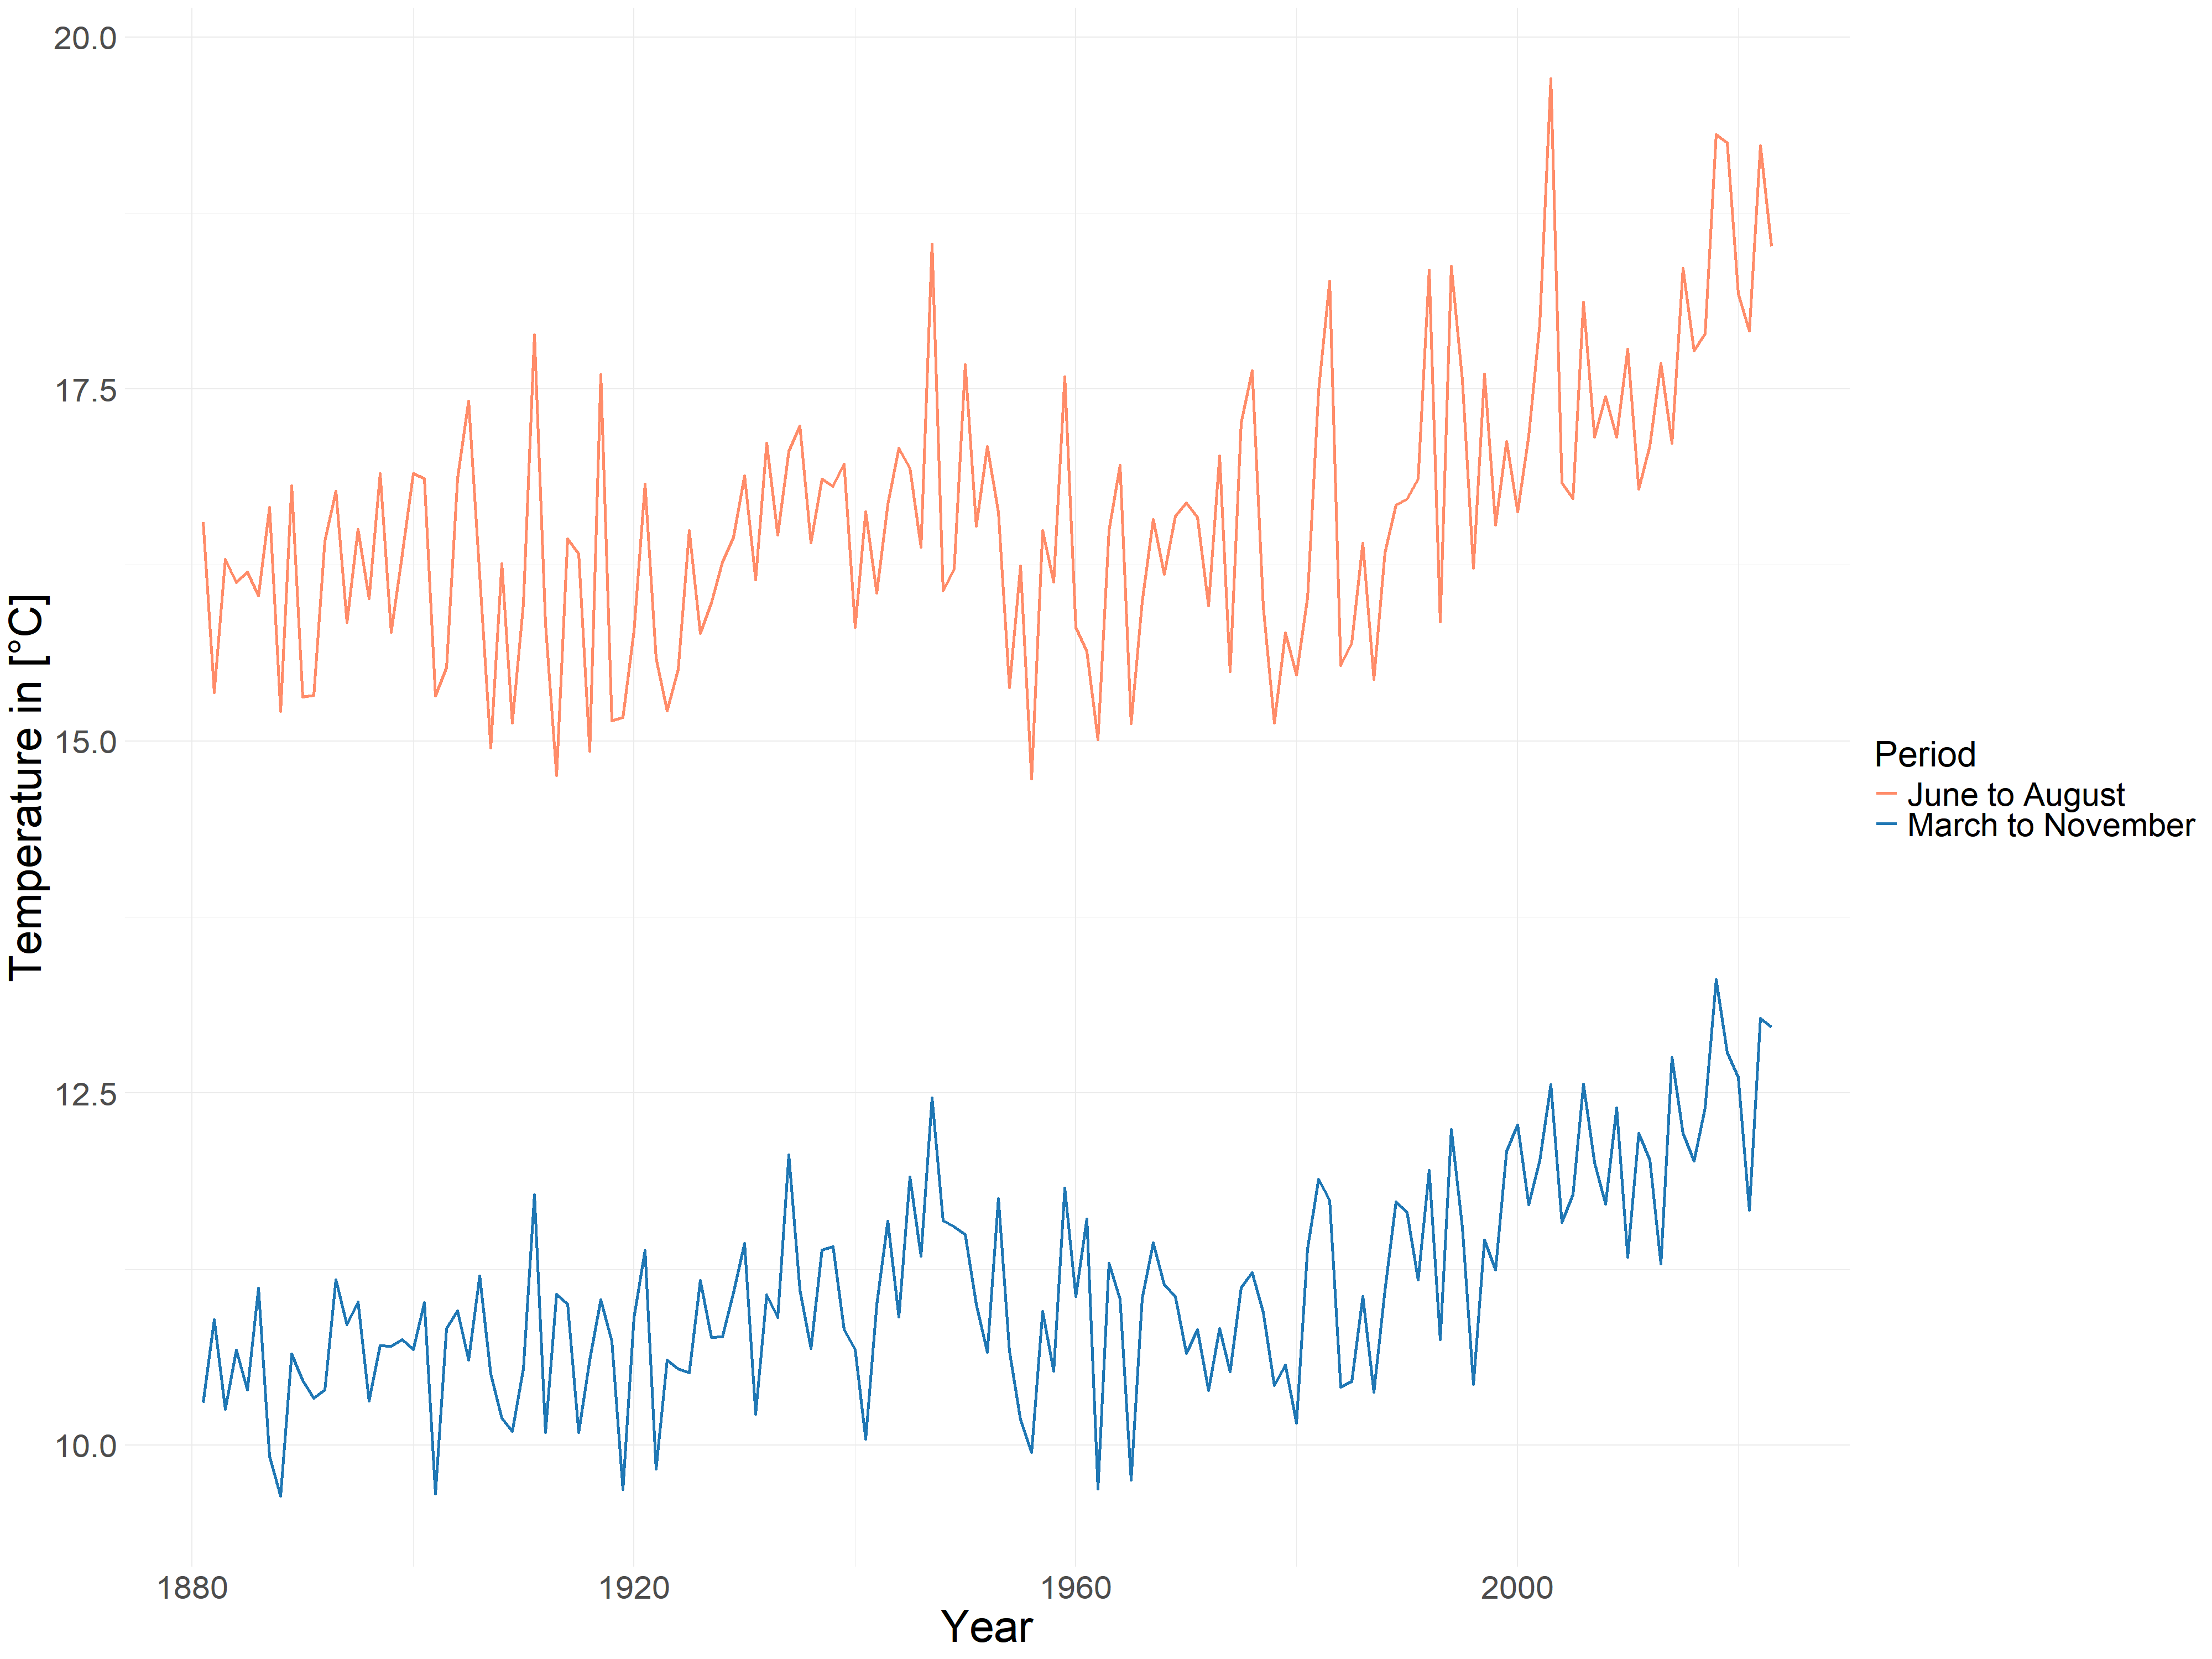
\includegraphics[width=0.7\linewidth]{work/03-compounds/figures/Temperature/Average/Temperature} 

}

\caption{Average Temperature in Germany from March to November and from June to August}\label{fig:AverageTemperature-shiyu}
\end{figure}

Now let's look at the precipitation in Figure \ref{fig:AveragePrecipitation-shiyu} , as a whole, there is no significant upward will downward trend in precipitation, it's very stable overall. In order to avoid misinterpretation, it should be noted that due to the different calculation methods, we cannot directly compare the amount of precipitation from March to November and from June to August because they have different time scales, and what we can compare is only the trend of both of them. Similarly, the amount of precipitation from March to November and June to August 2018 was very low.

\begin{figure}

{\centering 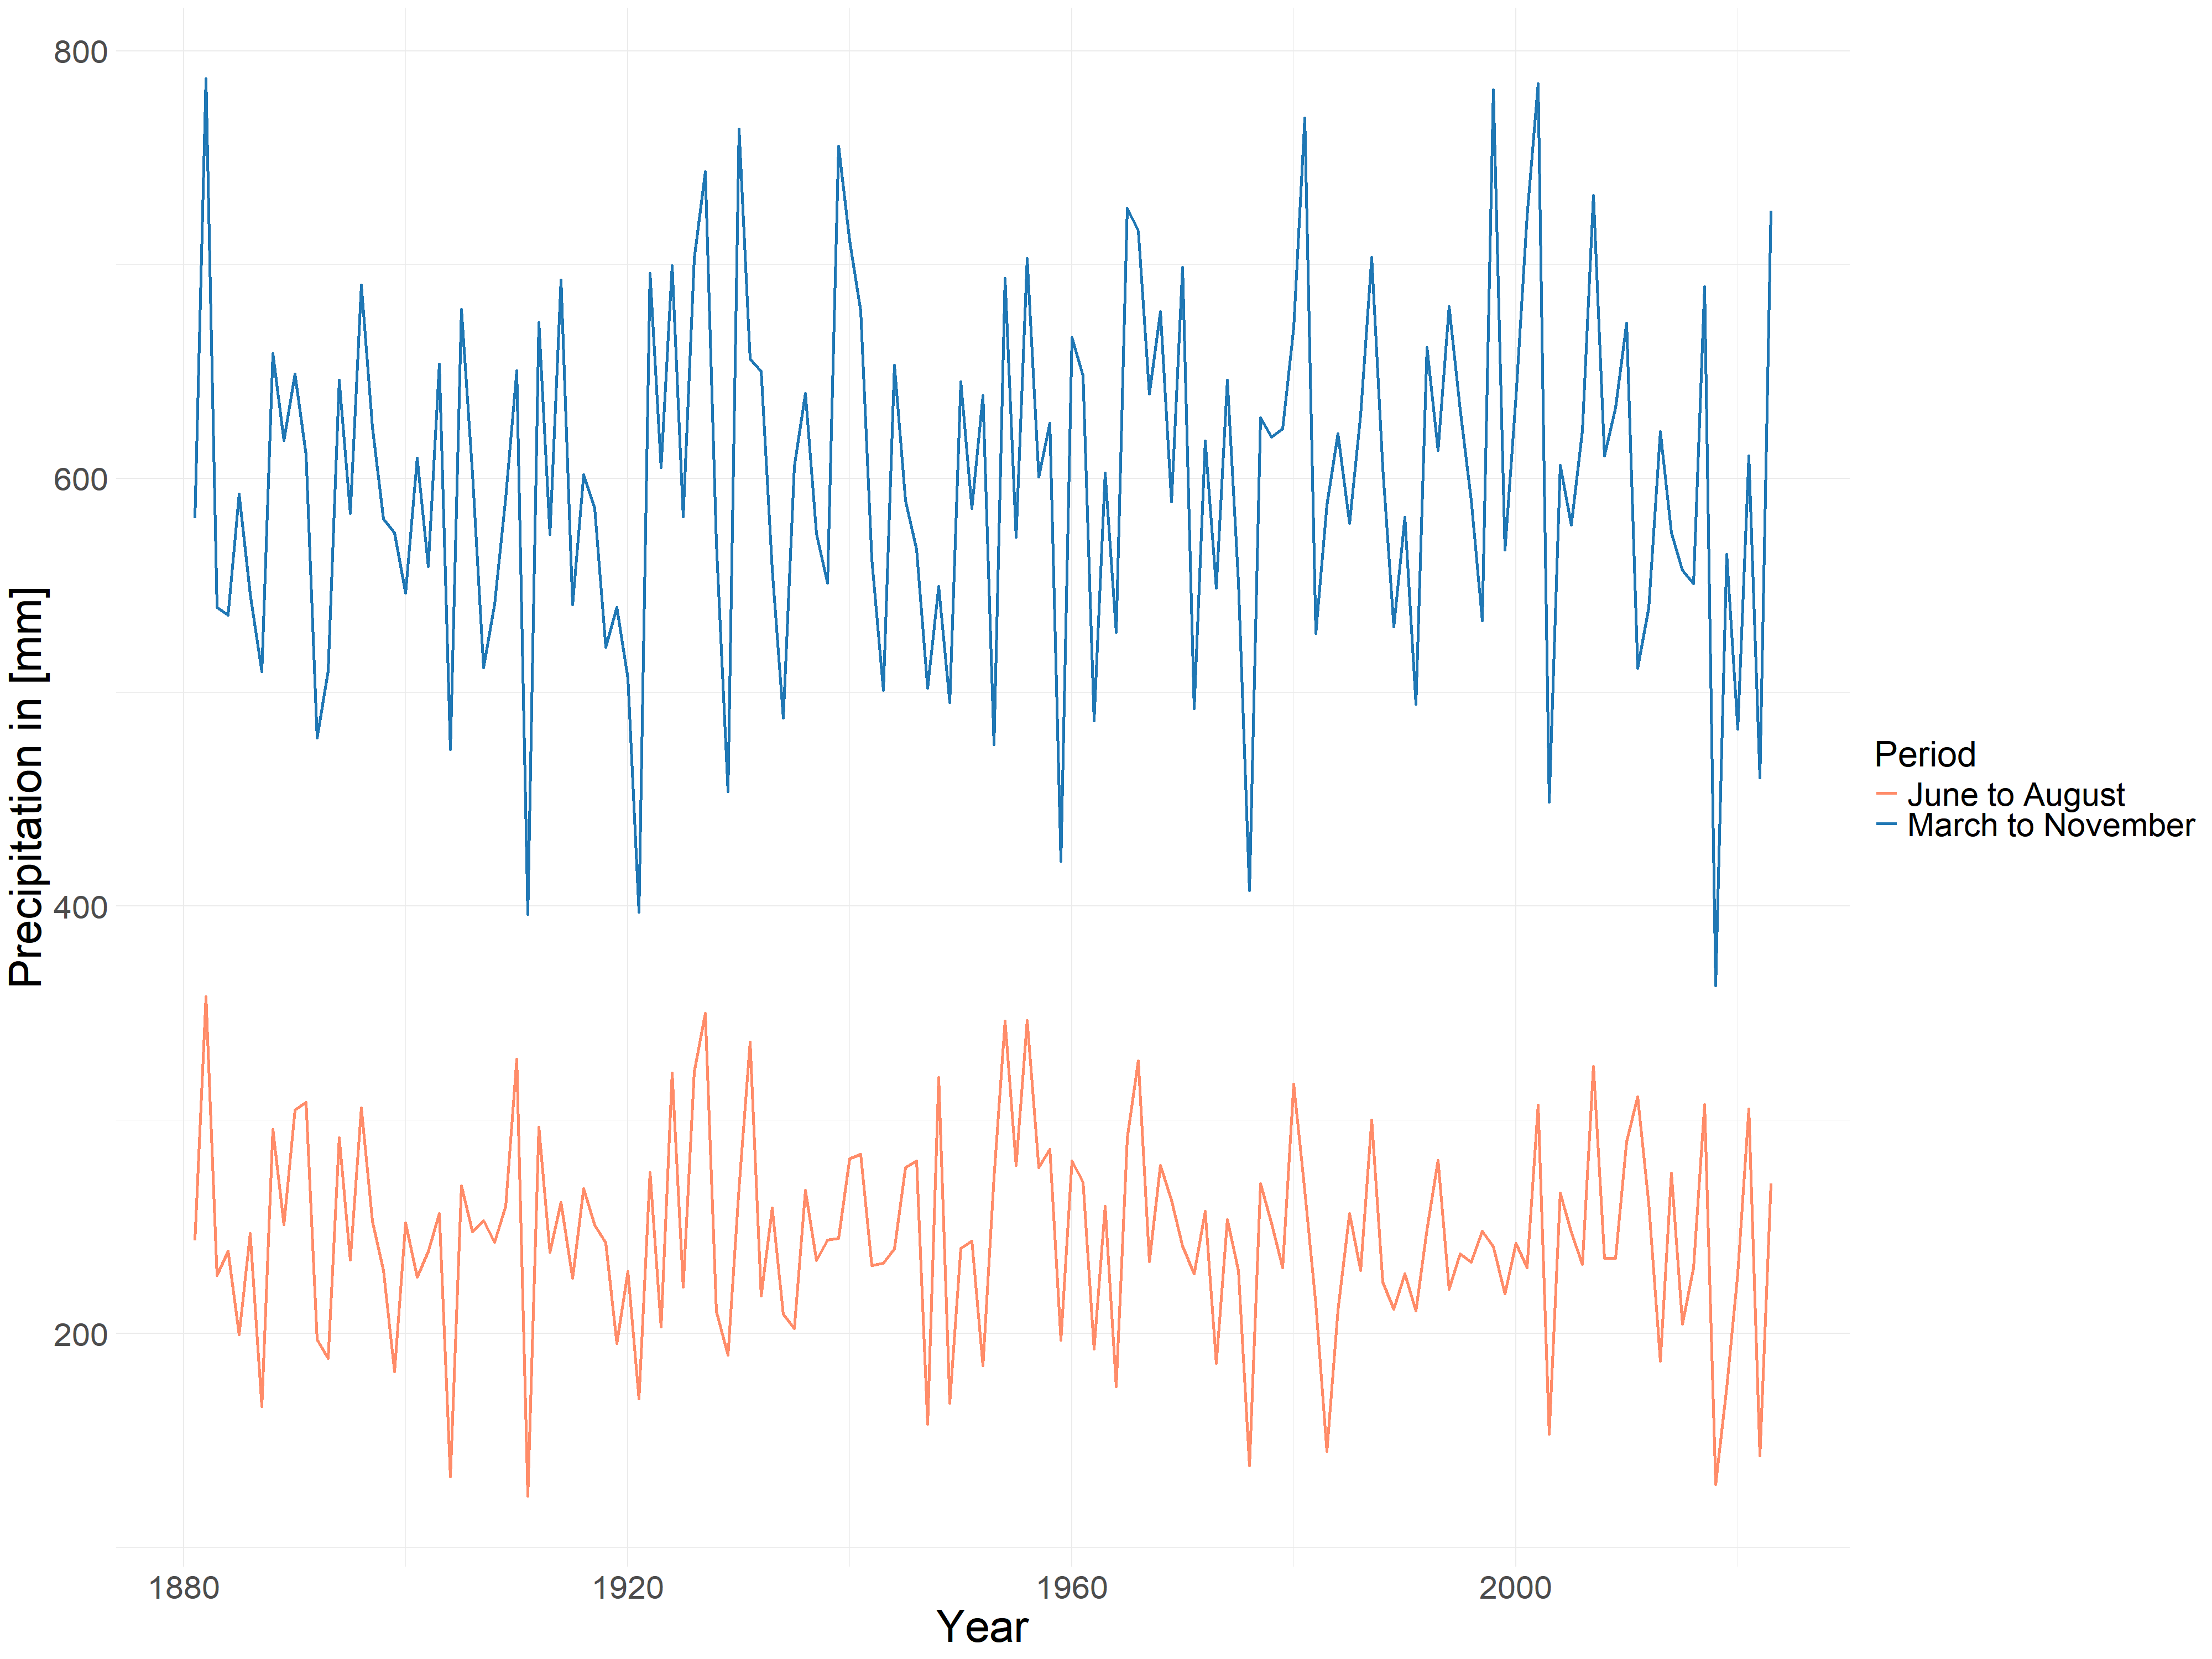
\includegraphics[width=0.7\linewidth]{work/03-compounds/figures/Precipitation/Average/Precipitation} 

}

\caption{Average Precipitation in Germany from March to November and from June to August}\label{fig:AveragePrecipitation-shiyu}
\end{figure}

Now we understand the changes of these two variables over time, but based on the previous introduction to Copula we can know that real data cannot be put into the Copula model for computation directly, so we have to compute the cumulative distribution function. The empirical cumulative distribution function and the fitted normal cumulative distribution function were used simultaneously, and the results obtained are shown in Figure \ref{fig:TemperatureCPD-shiyu}. and Figure \ref{fig:PrecipitationCPD-shiyu}.

\begin{figure}

{\centering 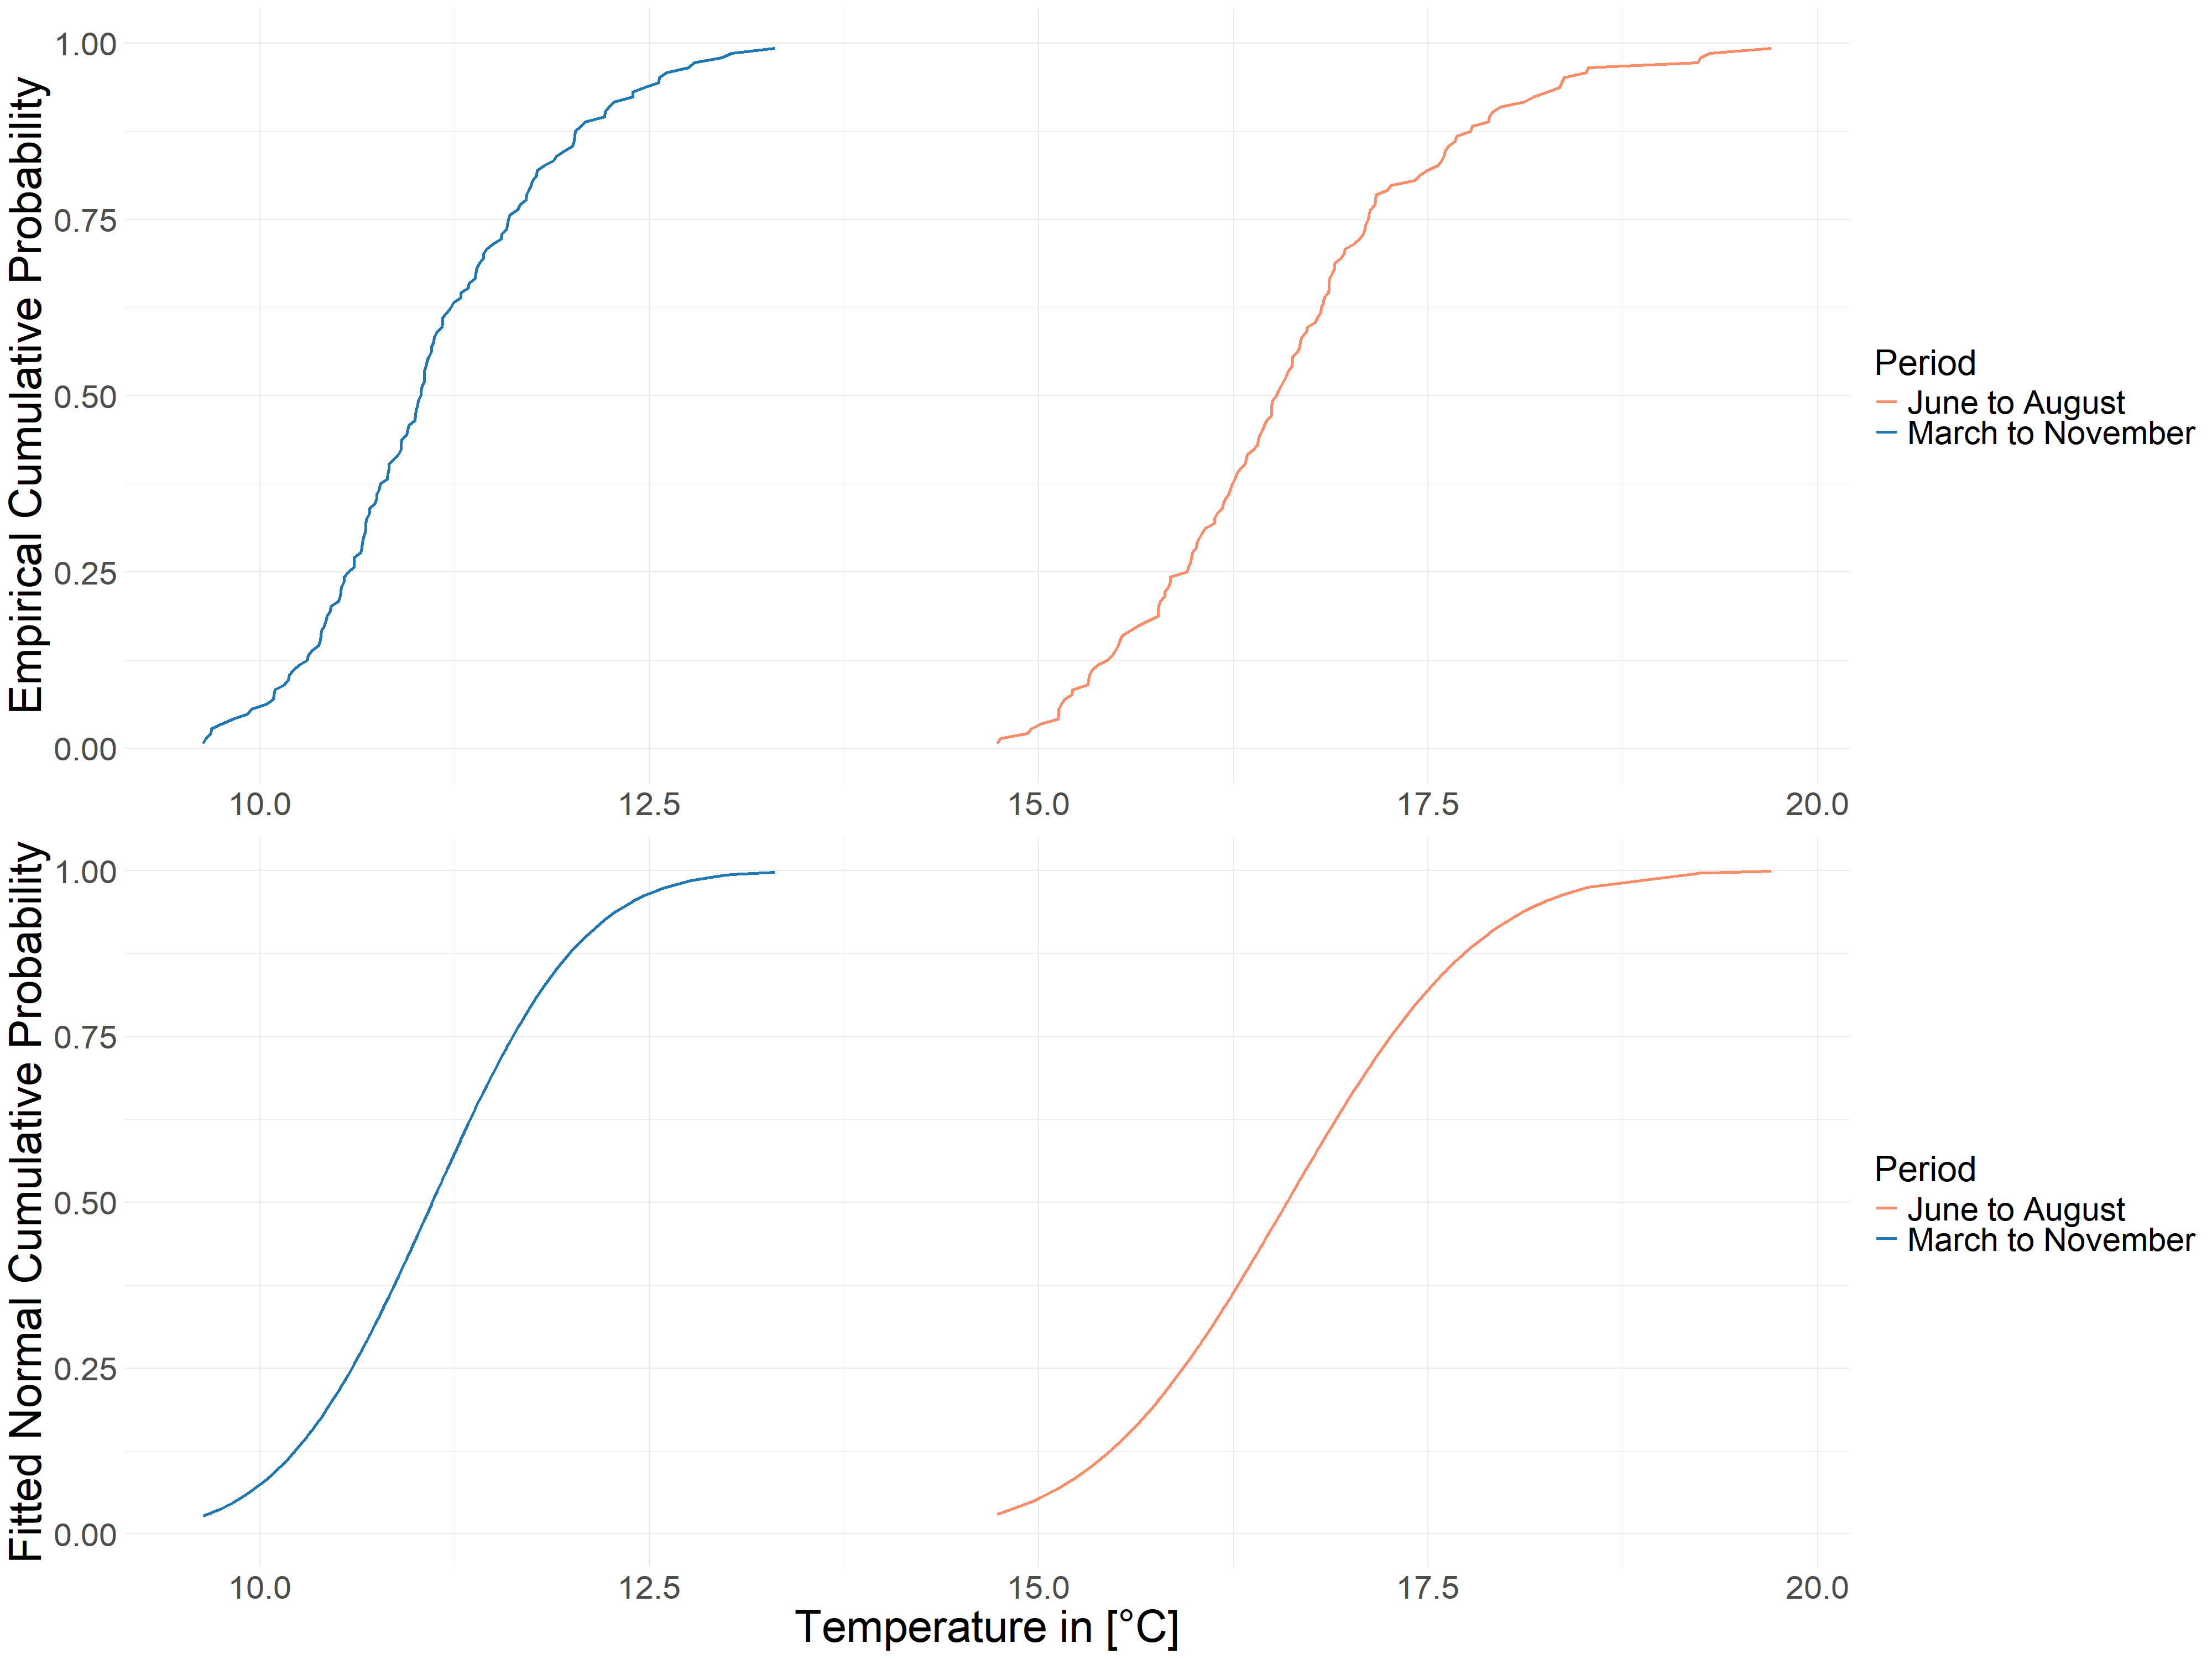
\includegraphics[width=0.65\linewidth]{work/03-compounds/figures/Temperature/Average/TemperatureCPD} 

}

\caption{Cumulative Probability of Temperature}\label{fig:TemperatureCPD-shiyu}
\end{figure}

In Figure \ref{fig:PrecipitationCPD-shiyu}, instead of using precipitation directly, we used negative precipitation, so the hottest and driest values mean that both our variables negative precipitation and temperature are at their maximum values, which is the reason why we introduce the Upper Tail Dependence in 4.3.1.

\begin{figure}

{\centering 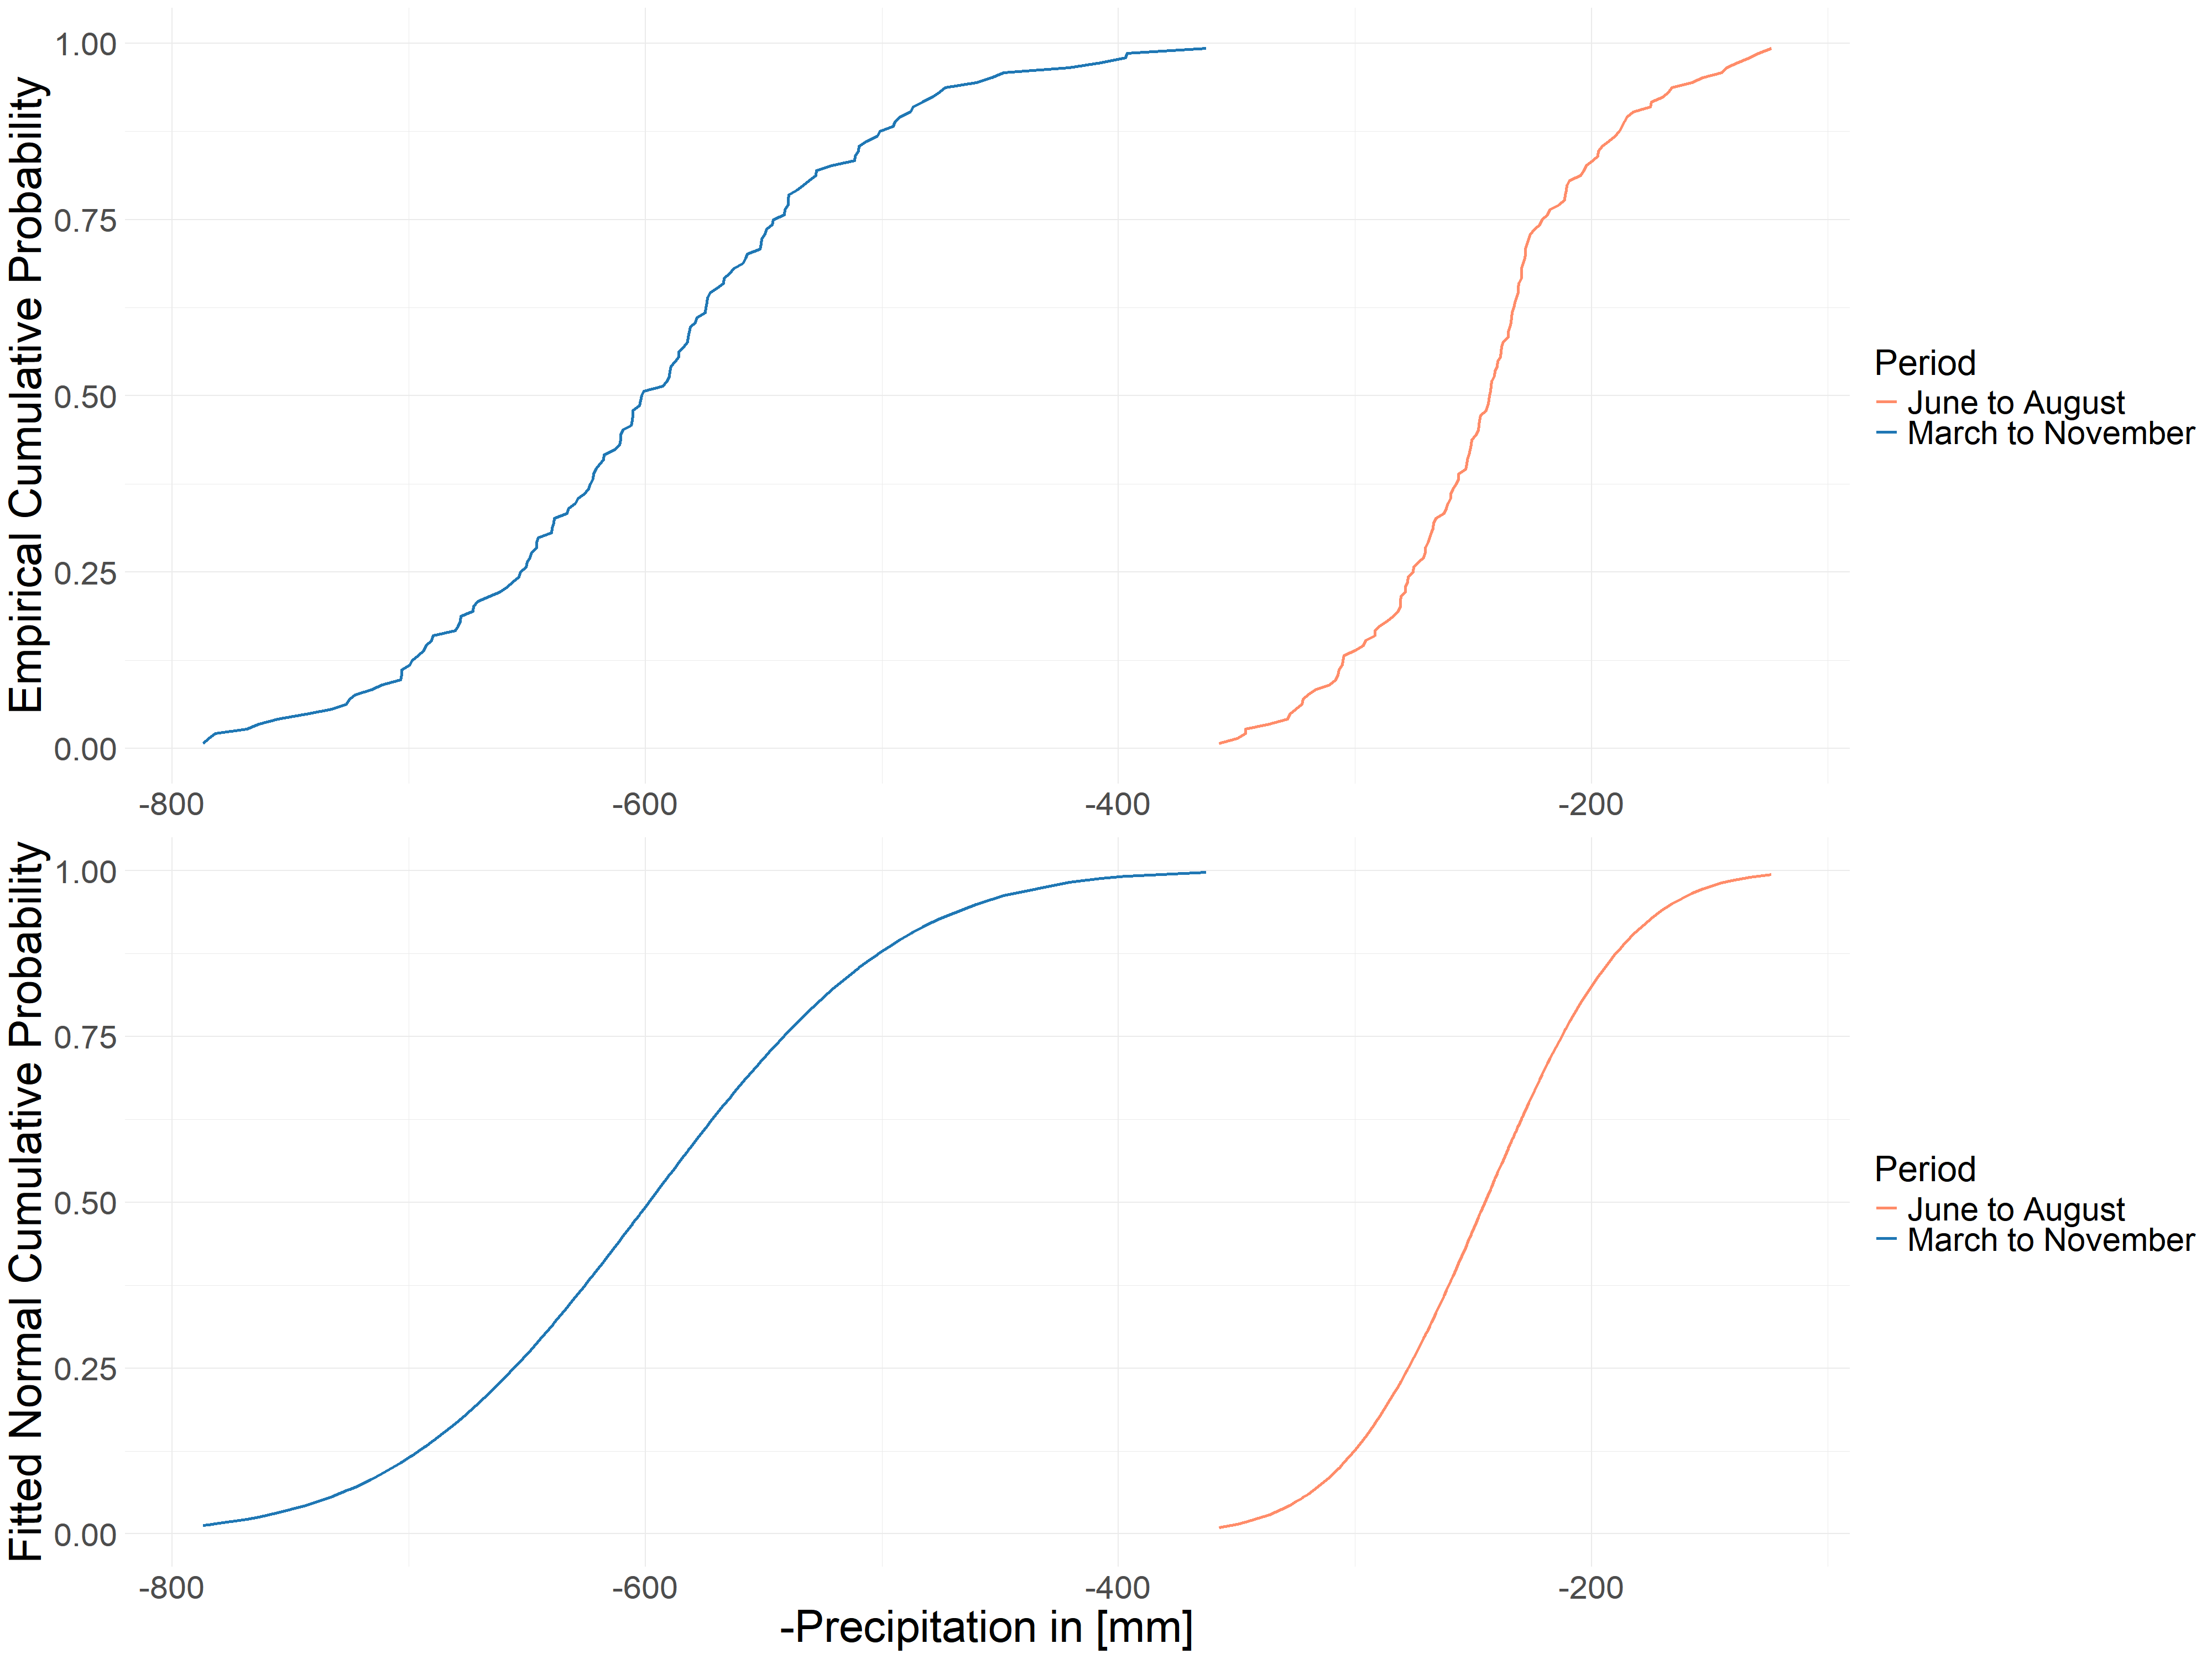
\includegraphics[width=0.65\linewidth]{work/03-compounds/figures/Precipitation/Average/PrecipitationCPD} 

}

\caption{Cumulative Probability of -Precipitation}\label{fig:PrecipitationCPD-shiyu}
\end{figure}

\subsection{Annual Global Mean Temperature Anomalies}\label{annual-global-mean-temperature-anomalies}

In addition, we introduce annual global mean temperature anomalies to estimate global mean temperature (GMT), which captures the global climate trend over the last 143 years. As can be seen from the increasing and steeper shape of the lines in Figure \ref{fig:gmt-shiyu}, global temperatures are really rising and at an increasing rate. However, the trends from June to August and March to November are very similar, suggesting that summers are not getting hotter faster compared to the entire growing season.

\begin{figure}

{\centering 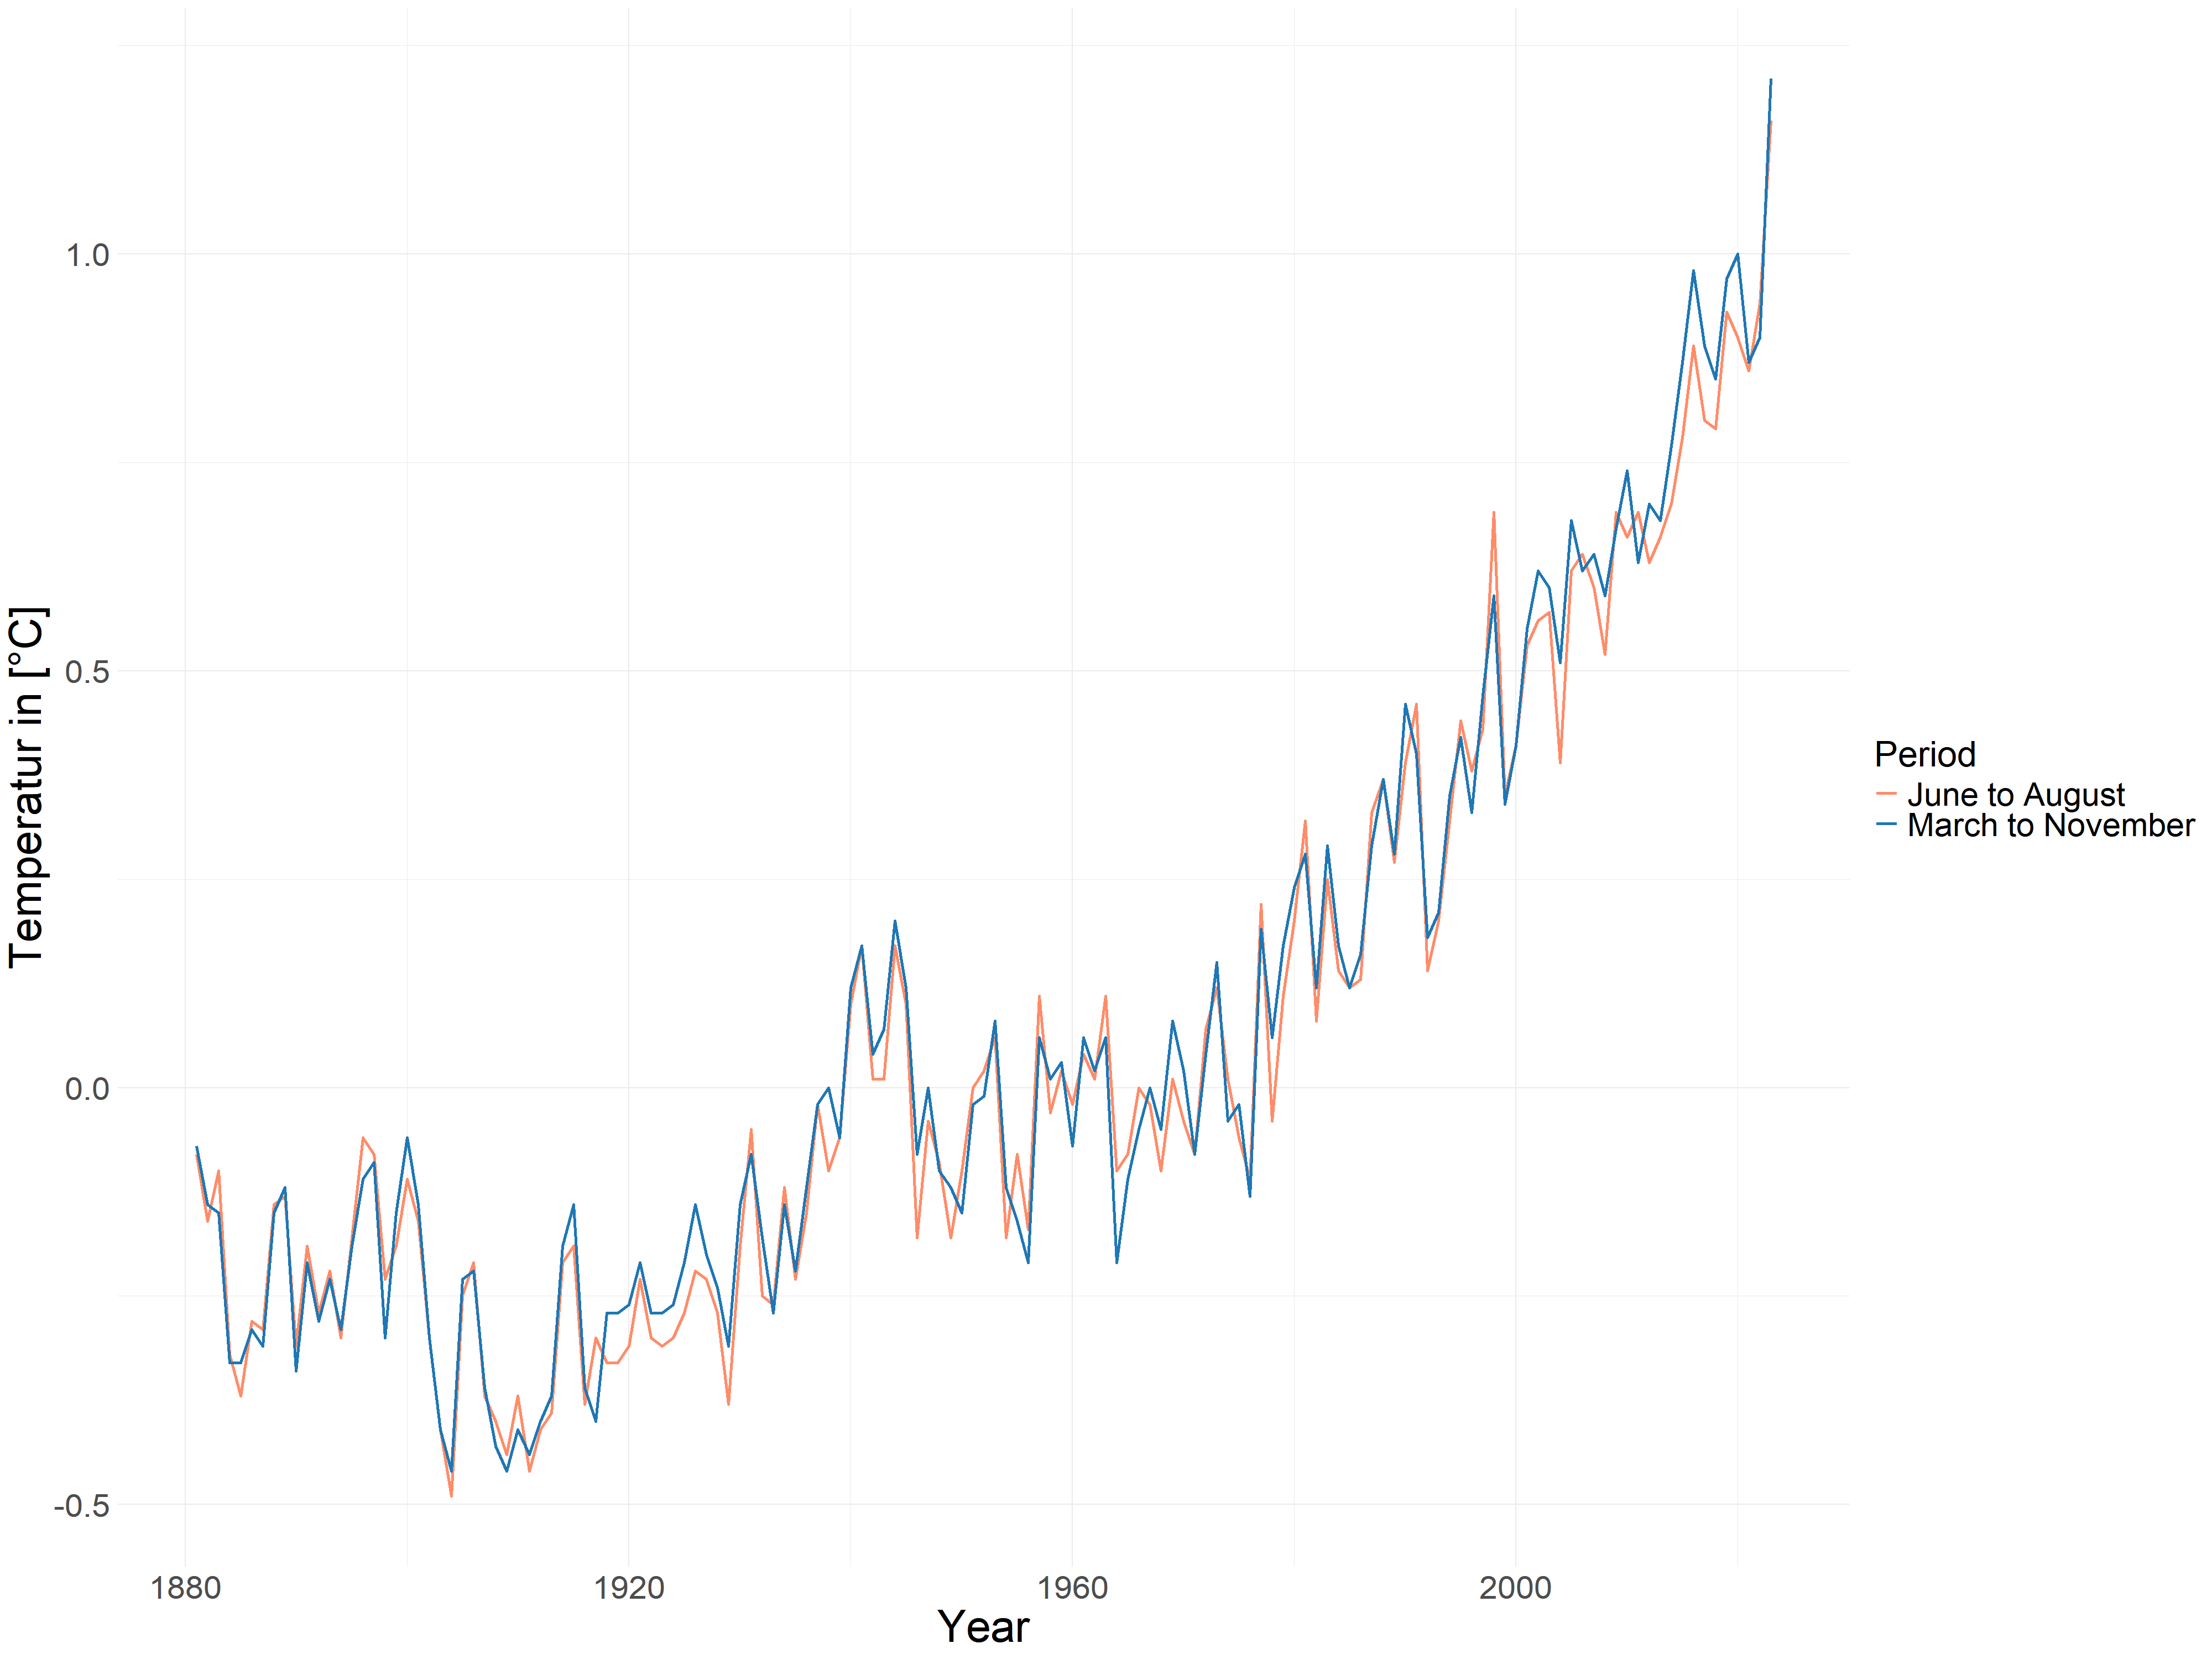
\includegraphics[width=0.7\linewidth]{work/03-compounds/figures/GMT/GMT} 

}

\caption{Annual Global Mean Temperature Anomalies from March to November and from June to August}\label{fig:gmt-shiyu}
\end{figure}

\section{Model}\label{model}

\subsection{Copula Models using Original data}\label{copula-models-using-original-data}

\begin{table}

\caption{\label{tab:tab1-shiyu}Marginal distributions and copulas for observational data (March-November averages)}
\centering
\begin{tabular}[t]{l|l|l|l}
\hline
 &  & EMP & FIT\\
\hline
Until 2019 & T & - & N(11, 0.7)\\
\hline
 & - P & - & N(-600, 84)\\
\hline
 & Copula & Joe(theta = 1.25) & Survival Clayton(theta = 0.26)\\
\hline
Until 2023 & T & - & N(11, 0.76)\\
\hline
 & - P & - & N(-599, 84)\\
\hline
 & Copula & Joe(theta = 1.31) & Joe(theta = 1.21)\\
\hline
 & Utd & 0.3 & 0.22\\
\hline
\end{tabular}
\end{table}

Table \ref{tab:tab1-shiyu} shows the marginal distributions and copulas for observational data in March to November. The data in the first row is from paper and is only updated to 2019, the data in the second row is updated to 2023, it is easy to see that the addition of 4 new years of data doesn't change the distribution of the data too much, which makes sense since there are over 100 years as a base. As mentioned in 4.2, here we used ``BiCopSelect()'' in the R package VineCopula (\citet{schepsmeier2018}) for the model selection, it is possible to set different selection criteria in this function, and here we used the default criterion Akaike information criterion (AIC). Different Copula models were chosen in 2019 and 2023, but at least they are all Copula's that are suitable for capturing UTD as mentioned in 4.3.3, I extracted their UTD values for the 2023 model and we can see that the UTD for the 2023 Copula model based on the empirical marginal distribution is 0.3, and the UTD of the Copula model based on the fitted normal marginal distribution is 0.22, which is not particularly strong, but already suggests a Upper Tail Dependence between hot and dry.

\begin{table}

\caption{\label{tab:tab2-shiyu}Best Copula Model (EMP) for different Bundesland (March to November)}
\centering
\begin{tabular}[t]{l|l|l|r}
\hline
shapeName & model & tau & UTD\\
\hline
Baden-Württemberg & Tawn type 1 & 0.18 ** & 0.23\\
\hline
Bayern & Joe & 0.15 ** & 0.30\\
\hline
Berlin & Joe & 0.13 * & 0.27\\
\hline
Brandenburg & Joe & 0.14 * & 0.29\\
\hline
Bremen & Joe & 0.1 & 0.22\\
\hline
Hamburg & Joe & 0.1 & 0.21\\
\hline
Hessen & Joe & 0.13 * & 0.27\\
\hline
Mecklenburg-Vorpommern & Joe & 0.13 & 0.26\\
\hline
Niedersachsen & Joe & 0.11 & 0.23\\
\hline
Nordrhein-Westfalen & Joe & 0.12 . & 0.26\\
\hline
Rheinland-Pfalz & Survival Clayton & 0.15 * & 0.13\\
\hline
Saarland & Survival Clayton & 0.13 * & 0.10\\
\hline
Sachsen & Survival Clayton & 0.23 *** & 0.31\\
\hline
Sachsen-Anhalt & Joe & 0.17 * & 0.33\\
\hline
Schleswig-Holstein & Independence & 0 & 0.00\\
\hline
Thüringen & Joe & 0.14 * & 0.29\\
\hline
\end{tabular}
\end{table}

\[\text{Signif. codes: 0 ‘***’ 0.001 ‘**’ 0.01 ‘*’ 0.05 ‘.’ 0.1 ‘ ’ 1}\]

At the level of Germany as a whole, the Copula model is performing well, so next we'll look at the Bundesland. The data obtained from the empirical marginal distributions are shown in Table \ref{tab:tab2-shiyu}, where we can see that Joe and Survival Clayton Copula are still chosen for most of the regions, and based on the tau it shows that there is a positive correlation between temperature and negative precipitation in almost all of the regions, i.e.~a negative correlation between temperature and precipitation. There is also a clear Upper Tail Dependence in almost all of the Bundesländer. Only in Schleswig-Holstein precipitation and temperature are considered uncorrelated.

\begin{table}

\caption{\label{tab:tab3-shiyu}Best Copula Model (FIT) for different Bundesland for (March to November)}
\centering
\begin{tabular}[t]{l|l|l|r}
\hline
shapeName & model & tau & UTD\\
\hline
Baden-Württemberg & Gumbel & 0.13 ** & 0.17\\
\hline
Bayern & t & 0.15 ** & 0.09\\
\hline
Berlin & Survival Clayton & 0.13 * & 0.09\\
\hline
Brandenburg & Survival Clayton & 0.14 * & 0.11\\
\hline
Bremen & Joe & 0.09 & 0.19\\
\hline
Hamburg & Joe & 0.09 & 0.19\\
\hline
Hessen & Survival Clayton & 0.11 * & 0.06\\
\hline
Mecklenburg-Vorpommern & Joe & 0.11 & 0.24\\
\hline
Niedersachsen & Joe & 0.08 & 0.18\\
\hline
Nordrhein-Westfalen & Survival Clayton & 0.11 . & 0.07\\
\hline
Rheinland-Pfalz & Survival Clayton & 0.11 * & 0.06\\
\hline
Saarland & Survival Clayton & 0.09 * & 0.03\\
\hline
Sachsen & Gumbel & 0.21 *** & 0.28\\
\hline
Sachsen-Anhalt & Joe & 0.14 * & 0.29\\
\hline
Schleswig-Holstein & Independence & 0 & 0.00\\
\hline
Thüringen & Joe & 0.11 * & 0.23\\
\hline
\end{tabular}
\end{table}

\[\text{Signif. codes: 0 ‘***’ 0.001 ‘**’ 0.01 ‘*’ 0.05 ‘.’ 0.1 ‘ ’ 1}\]

In Table \ref{tab:tab3-shiyu}, which shows the data obtained according to the fitted marginal distributions and compares the two tables, it can be seen that the tau values do not change much, that means the overall correlation between the variables does not change particularly much, regardless of which distribution is used. However, UTD seems to be very much affected, and the results of the comparison can be more visualized through Figure \ref{fig:utdmap1-shiyu}.

\begin{figure}

{\centering 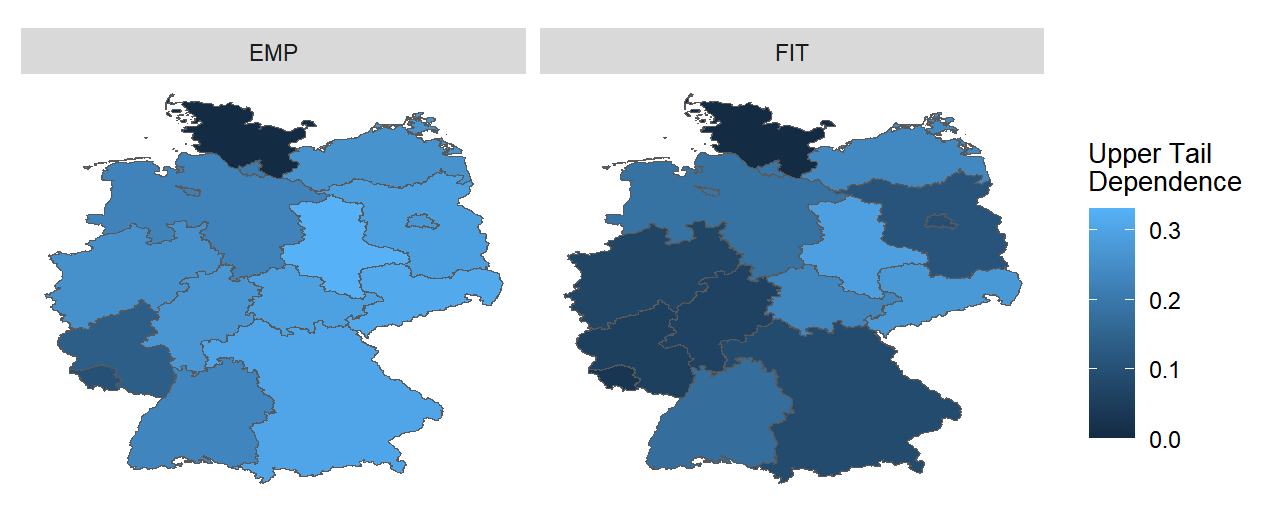
\includegraphics[width=0.8\linewidth]{work/03-compounds/figures/UTDMAP/original} 

}

\caption{Upper Tail Dependence in different Bundesland from March to November (Original))}\label{fig:utdmap1-shiyu}
\end{figure}

Only Sachsen-Anhalt, Sachsen and Mecklenburg-Vorpommern remain relatively high in UTD, with Bayern, Hessen, and the surrounding area all having low UTD. This result is very unpromising, as we have to use data obtained according to the fitted marginal distribution for subsequent studies. The reason for this result may be due to that the difference between the extreme values in the data and their closest values is also very large, and thus the probability that the parameter fit assigns an extreme value becomes smaller thus affecting the UTD. So we need to find ways to standardize the raw data even more.

\subsection{Copula Models using Anomalies}\label{copula-models-using-anomalies}

Now, we introduce the GMT, which estimated by annual global mean temperature anomalies, to process the raw data in order to remove the effect of global temperature change on regional temperature and precipitation. First we model GMT and temperature and precipitation with the simplest linear model to get the following two models, then we use the real data to subtract the estimates of temperature and precipitation from these two models to get the data we will use later, which we call Anomalies.

\[\text{Temperature} = 11 + 1.41 * \text{GMT} \tag{21}\]
\[\text{Precipitation} = 597.71 + 13.04 * \text{GMT} \tag{22}\]

With the new data, we can find that the selected models still all good at capturing UTD. And comparing the UTD values of the two sets of models in Table \ref{tab:tab1-shiyu} and Table \ref{tab:tab4-shiyu}, it is easy to see that the Copula model using Anomalies has improved.

\begin{table}

\caption{\label{tab:tab4-shiyu}Marginal distributions and copulas for Anomalies (March-November averages)}
\centering
\begin{tabular}[t]{l|l|l|l}
\hline
 &  & EMP & FIT\\
\hline
Anomalies & T & - & N(0, 0.5)\\
\hline
 & -P & - & N(0, 83)\\
\hline
 & Copula & Survival Clayton (theta = 0.61) & Survival Clayton(theta = 0.56)\\
\hline
Anomalies & T & - & N(0, 0.55)\\
\hline
 & -P & - & N(0, 84)\\
\hline
 & Copula & Joe(theta = 1.53) & Survival Clayton(theta = 0.58)\\
\hline
 & UTD & 0.43 & 0.3\\
\hline
\end{tabular}
\end{table}

Then looking again to Bundesland, in Table \ref{tab:tab5-shiyu} both tau and UTD have improved with respect to the previous data in Table \ref{tab:tab2-shiyu}, and even in Schleswig-Holstein now shows a correlation between the two variables.

\begin{table}

\caption{\label{tab:tab5-shiyu}Best Copula Model (EMP) for different Bundesland (March to November Anomalies)}
\centering
\begin{tabular}[t]{l|l|l|r}
\hline
shapeName & model & tau & UTD\\
\hline
Baden-Württemberg & Survival Clayton & 0.24 *** & 0.34\\
\hline
Bayern & Joe & 0.27 *** & 0.48\\
\hline
Berlin & Survival Clayton & 0.2 *** & 0.26\\
\hline
Brandenburg & Survival Clayton & 0.2 ** & 0.26\\
\hline
Bremen & Survival Clayton & 0.16 . & 0.16\\
\hline
Hamburg & Joe & 0.17 * & 0.33\\
\hline
Hessen & Joe & 0.2 ** & 0.38\\
\hline
Mecklenburg-Vorpommern & Survival Clayton & 0.16 * & 0.16\\
\hline
Niedersachsen & Survival Clayton & 0.19 * & 0.22\\
\hline
Nordrhein-Westfalen & Survival Clayton & 0.22 ** & 0.29\\
\hline
Rheinland-Pfalz & Survival Clayton & 0.22 *** & 0.30\\
\hline
Saarland & Survival Clayton & 0.22 *** & 0.30\\
\hline
Sachsen & Survival Clayton & 0.27 *** & 0.40\\
\hline
Sachsen-Anhalt & Joe & 0.22 *** & 0.42\\
\hline
Schleswig-Holstein & Survival Clayton & 0.13 & 0.10\\
\hline
Thüringen & Joe & 0.24 *** & 0.44\\
\hline
\end{tabular}
\end{table}

\[\text{Signif. codes: 0 ‘***’ 0.001 ‘**’ 0.01 ‘*’ 0.05 ‘.’ 0.1 ‘ ’ 1}\]

In Table \ref{tab:tab6-shiyu}, the overall lowering of UTD has also become smaller, but Rheinland-Pfalz and Saarland, while still maintaining kendalls tau, have lost UTD, but this is much more acceptable compared to the previous overall sharp fall.

\begin{table}

\caption{\label{tab:tab6-shiyu}Best Copula Model (FIT) for different Bundesland (March to November Anomalies)}
\centering
\begin{tabular}[t]{l|l|l|r}
\hline
shapeName & model & tau & UTD\\
\hline
Baden-Württemberg & Survival Clayton & 0.23 *** & 0.31\\
\hline
Bayern & Joe & 0.26 *** & 0.47\\
\hline
Berlin & Survival Clayton & 0.2 *** & 0.25\\
\hline
Brandenburg & Survival Clayton & 0.19 ** & 0.24\\
\hline
Bremen & Tawn type 1 & 0.06 . & 0.07\\
\hline
Hamburg & Survival Clayton & 0.17 * & 0.18\\
\hline
Hessen & Survival Clayton & 0.19 ** & 0.24\\
\hline
Mecklenburg-Vorpommern & Survival Clayton & 0.16 * & 0.15\\
\hline
Niedersachsen & Survival Clayton & 0.17 * & 0.18\\
\hline
Nordrhein-Westfalen & Survival Clayton & 0.2 ** & 0.24\\
\hline
Rheinland-Pfalz & BB8 & 0.23 *** & 0.00\\
\hline
Saarland & BB8 & 0.22 *** & 0.00\\
\hline
Sachsen & Survival Clayton & 0.27 *** & 0.38\\
\hline
Sachsen-Anhalt & Joe & 0.22 *** & 0.41\\
\hline
Schleswig-Holstein & Survival Clayton & 0.12 & 0.07\\
\hline
Thüringen & Joe & 0.22 *** & 0.41\\
\hline
\end{tabular}
\end{table}

\[\text{Signif. codes: 0 ‘***’ 0.001 ‘**’ 0.01 ‘*’ 0.05 ‘.’ 0.1 ‘ ’ 1}\]

As can also be seen in Figure \ref{fig:utdmap2-shiyu}, the differences in EMP and FIT-related data between Sachsen and Sachens Anhalt are still relatively small, while the differences in regions such as Bayern and Thuringen are not as clearly visible as they were in Figure \ref{fig:utdmap1-shiyu}.

\begin{figure}

{\centering 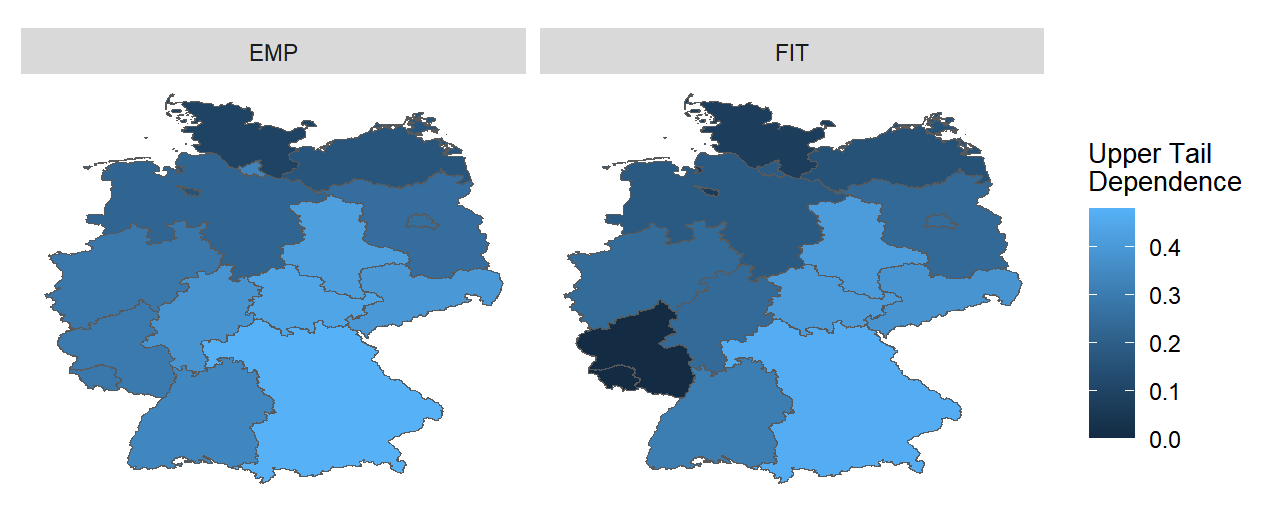
\includegraphics[width=0.8\linewidth]{work/03-compounds/figures/UTDMAP/anomalies} 

}

\caption{Upper Tail Dependence in different Bundesland from March to November (Anomalies))}\label{fig:utdmap2-shiyu}
\end{figure}

When we look at the data from June to August only, we can see that the situation is very similar to that of March to November, and Anomalies can be also very helpful.

\section{Rarity of 2018}\label{rarity-of-2018}

\subsection{From March to November}\label{from-march-to-november}

Next we use the model as a basis to study hot and dry, and here we need to review the four hazard scenarios mentioned in 4.3.4 and follow the criteria from \citet{zscheischler2020}, i.e by using the 2018 data as threshold to calculate the \(\text{P}_\text{AND}\), \(\text{P}_\text{OR}\), \(\text{P}_\text{K}\) and \(\text{P}_\text{SK}\).

\begin{figure}

{\centering 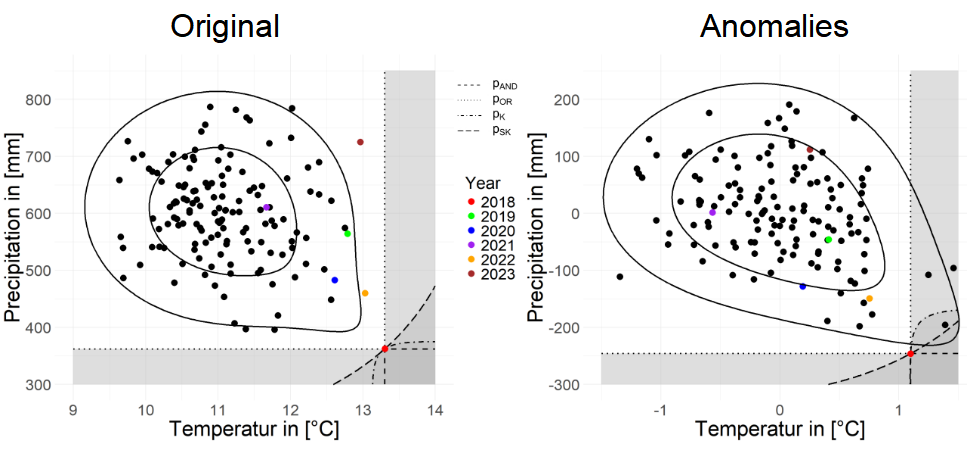
\includegraphics[width=0.8\linewidth]{work/03-compounds/figures/RESULTS/resultallMtoN} 

}

\caption{Rarity of 2018 for whole Germany from March to November}\label{fig:result1-shiyu}
\end{figure}

Each point in Figure \ref{fig:result1-shiyu} represents one year, 2018 as threshold is marked with a red point, while each year after 2018 is represented by other different colors, respectively. The contour lines are plotted according to the fitted copula model mentioned earlier and illustrate the copula at the levels 0.001 and 0.0001. The 4 different types of dotted lines and their corresponding shaded parts here represent the 4 hazard scenarios. We can see that the intersection of the four dotted lines is the point of the 2018 data. The left figure uses original data and the right figure uses Anomalies.
Looking at the figure of the original data, 2018 is indeed unquestionably the driest and hottest, and no other year can touch any of the four hazard scenarios. But when we look at the Anomalies data, we can find that 2018 is no longer the hottest year, which suggests that the high temperatures in Germany in 2018 were largely influenced by global heat. There were other years that came into the hazard scenario, but none of them are recent years.
Looking at the points for the most recent years of original data, we see that temperatures in 2022 and 2023, while not part of any hazardous scenarios, are higher than all other years except 2018. 2023 is relatively very wet, but 2022 is also relatively dry, in line with what the \citet{wmo2023b} said in its report about the European state for 2022. But the high temperatures in Germany in the past two years have also been largely influenced by the global heat.

\begin{figure}

{\centering 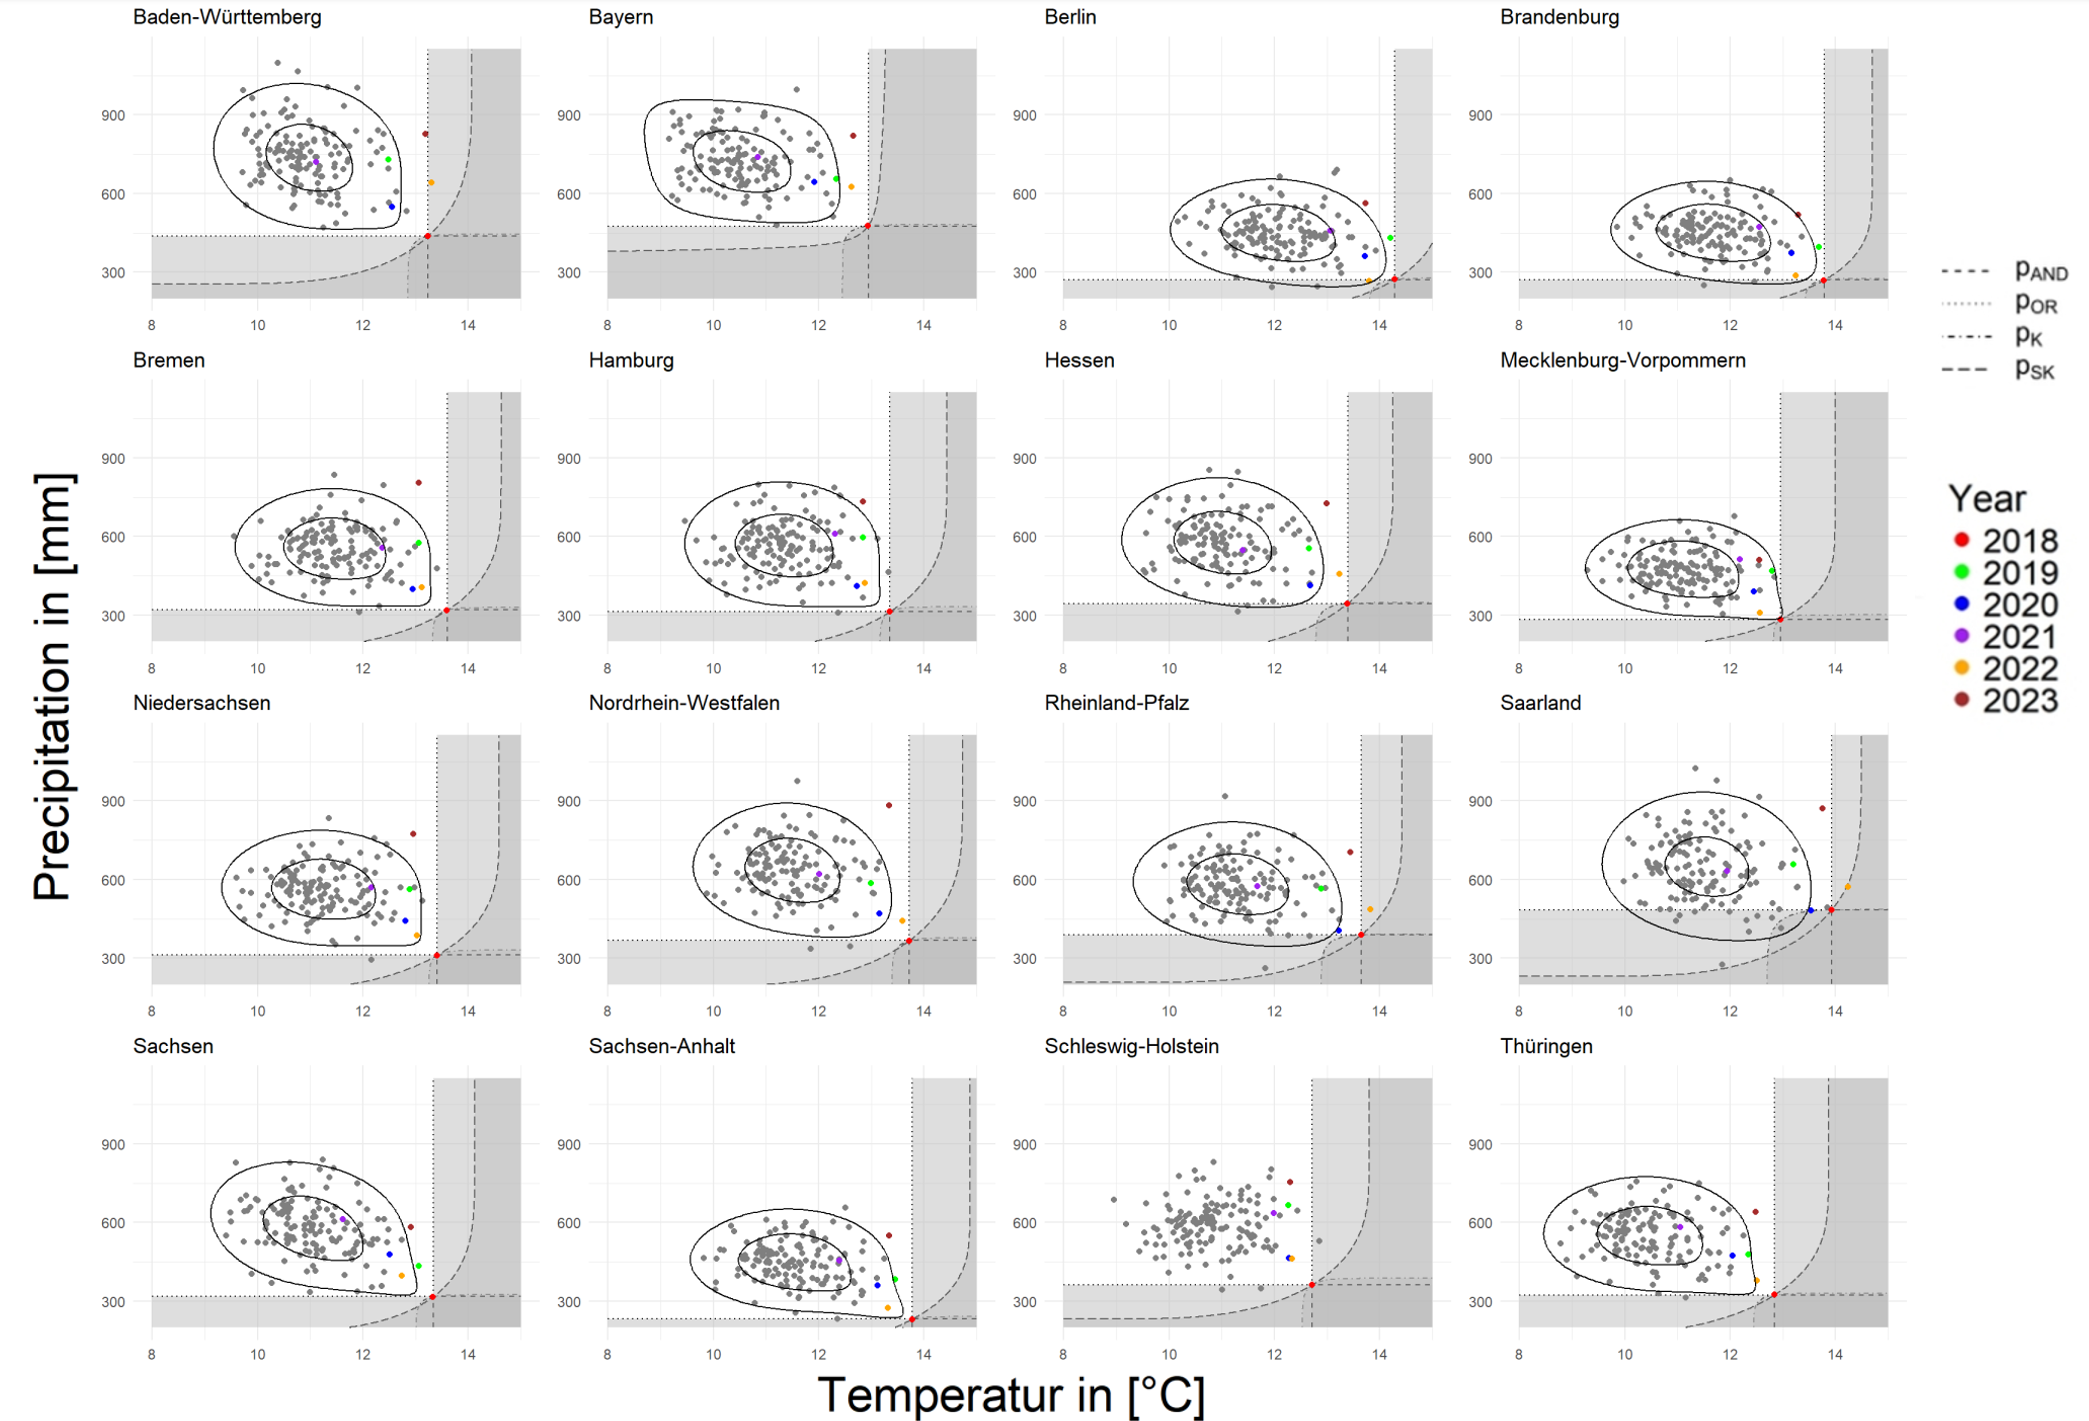
\includegraphics[width=0.8\linewidth]{work/03-compounds/figures/RESULTS/resultMtoN} 

}

\caption{Rarity of 2018 for Bundesland from March to November}\label{fig:result2-shiyu}
\end{figure}

Moving on to the situation in all Bundesland, we can see in Figure \ref{fig:result2-shiyu} that 2018 can be an special year for all Bundesland from the original data point of view, there may be some regions that will have other years that exceed 2018 on one single variable, but in general, 2018 was still a very hot and dry year. 2022 was very hot for many regions, and for Baden the last two years have both been very hot. Also we can notice that the three states of Berlin, Brandenburg and Sachsen Anhalt, as we learned from the map in 4.4.1, are the three hottest and driest states.
When looking at the Anomalies data, there is a large amount of data that appears in the shadow of hazard scenarios, and even in parts of the country there are years that are drier as well as hotter than 2018, and this can be seen especially in Saarland, but in none of region has a situation in recent years that was hotter and drier than 2018.

\begin{figure}

{\centering 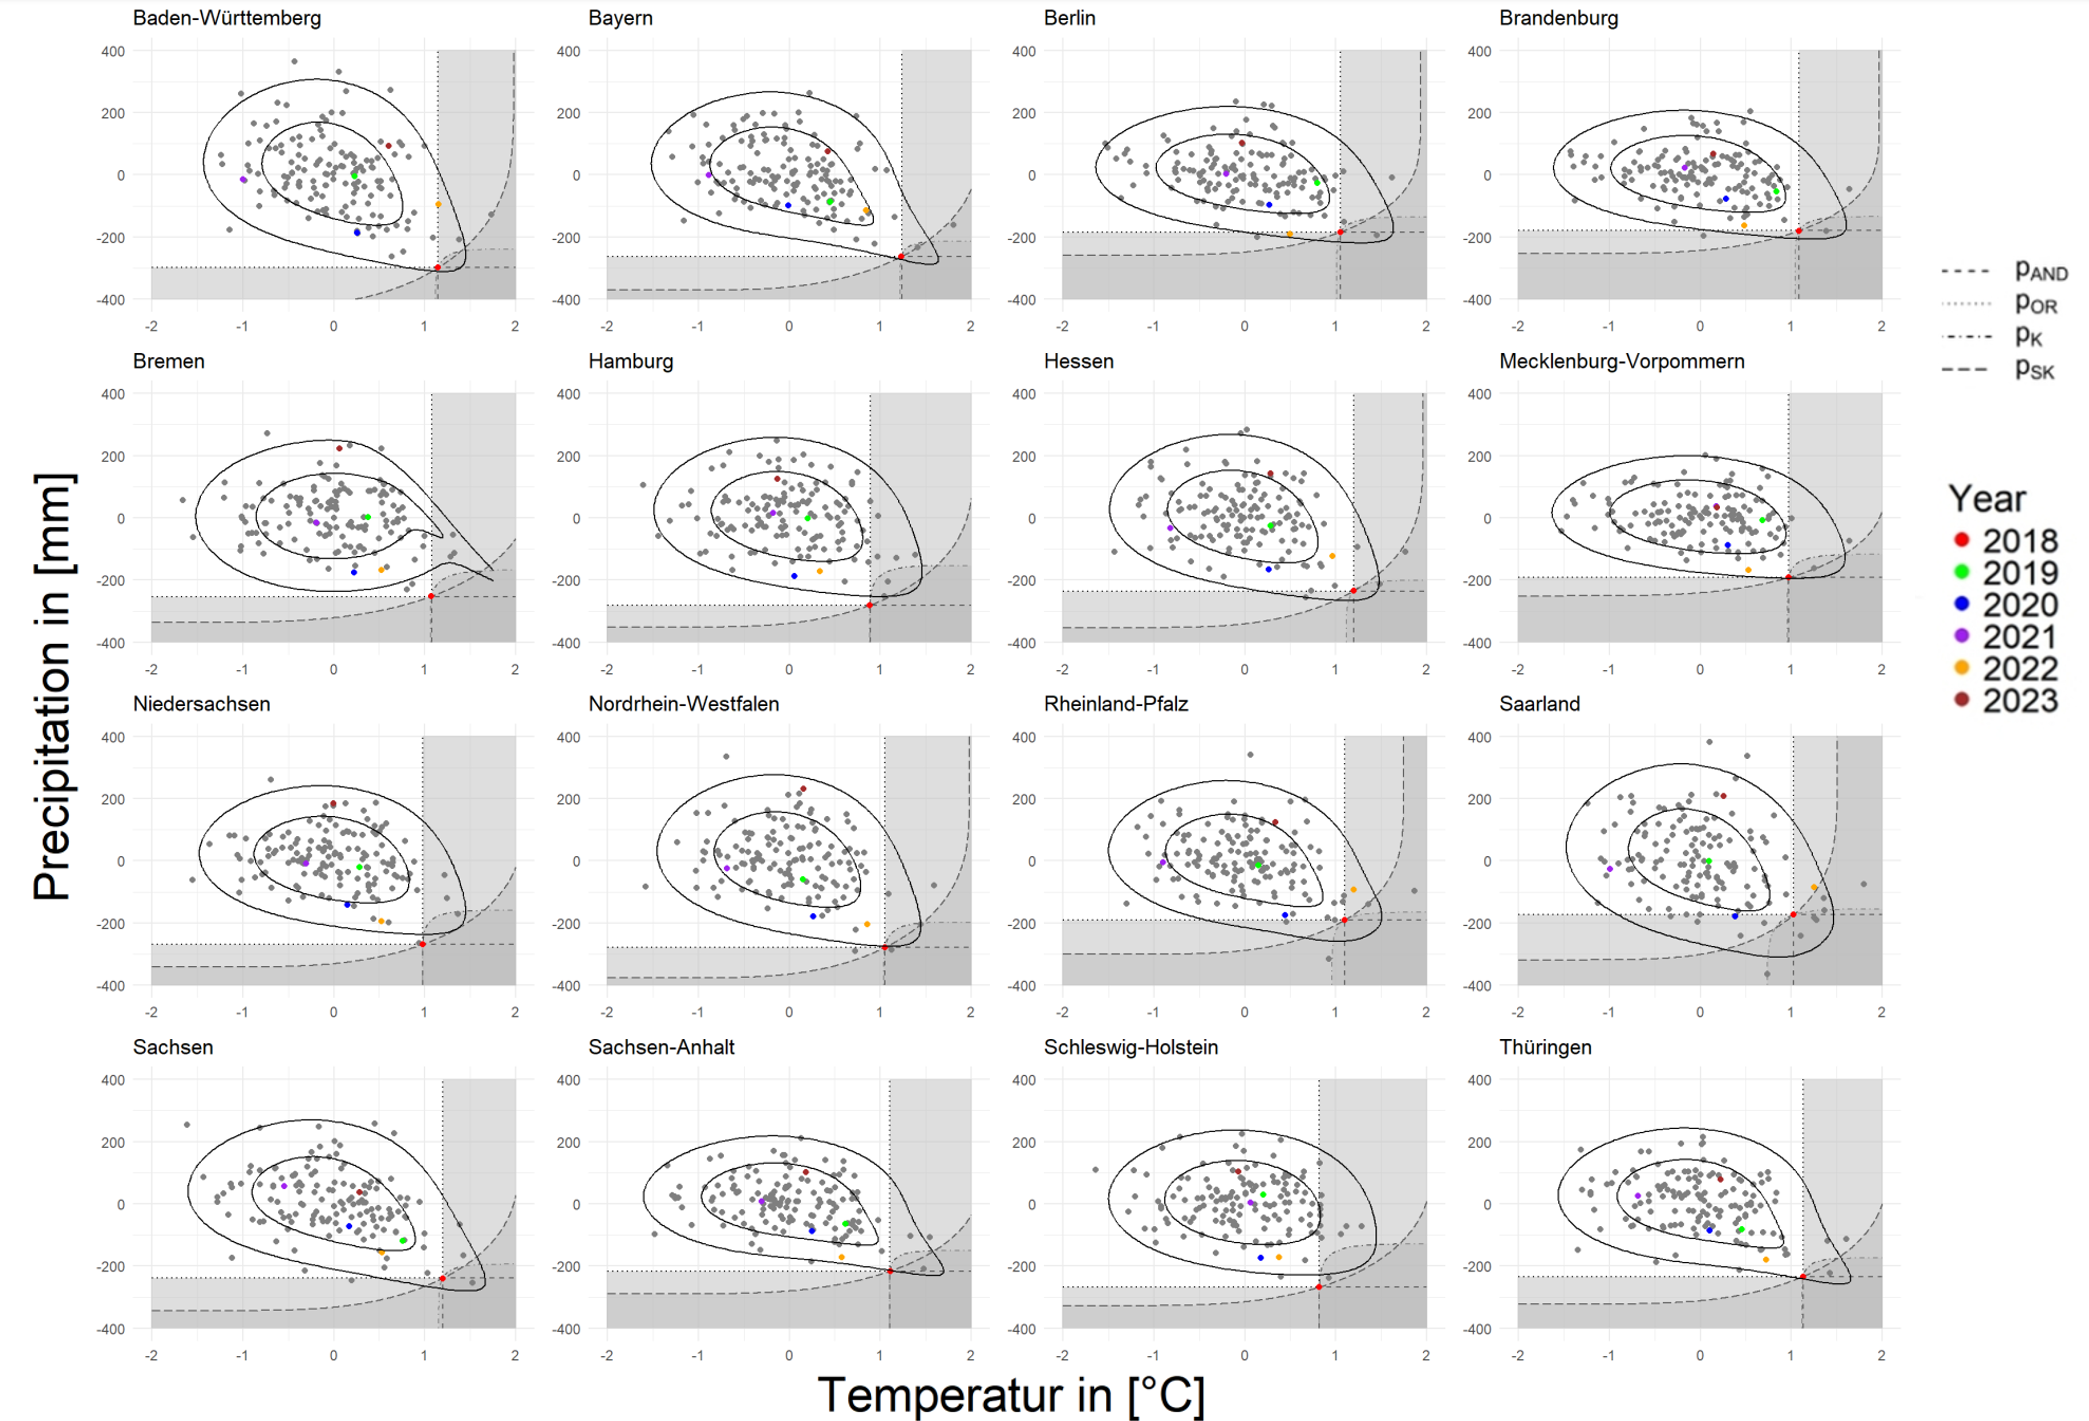
\includegraphics[width=0.8\linewidth]{work/03-compounds/figures/RESULTS/resultMtoNA} 

}

\caption{Rarity of 2018 for Bundesland from March to November (Anomalies)}\label{fig:result3-shiyu}
\end{figure}

When looking at the Anomalies data in Figure \ref{fig:result3-shiyu}, there is a large amount of data that appears in the shadow of hazard scenarios, and even in parts of the country there are years that are drier as well as hotter than 2018, and this can be seen especially in Saarland, but in none of region has a situation in recent years that was hotter and drier than 2018.

Saarland has a UTD of 0 in the Anomalies data. Looking at the figure in more detail, we can see that there is a lot of data for either dry-only or hot-only conditions. This makes the distribution of data in the bottom-right corner to be less concentrated and may lead to the driest and hottest conditions here being not significant. Sachsen - Anhalt is the Bundesland with a very strong UTD in the table, it is also clear in the graph that the values here close to 2018, although not as many as Saarland, are more concentrated and better able to fulfil both hot and dry.

\subsection{From June to August}\label{from-june-to-august}

\begin{figure}

{\centering 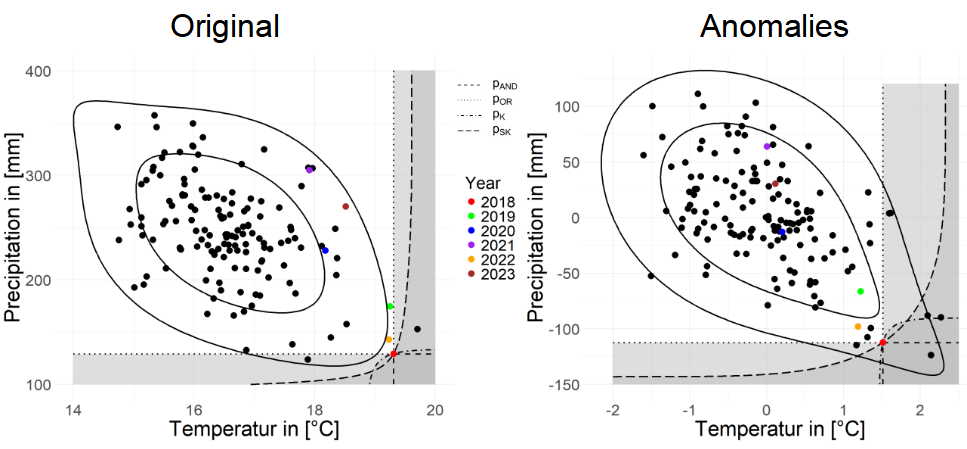
\includegraphics[width=0.8\linewidth]{work/03-compounds/figures/RESULTS/resultallJJA} 

}

\caption{Rarity of 2018 for whole Germany from June to August}\label{fig:result4-shiyu}
\end{figure}

Next let's look at the summer in Figure \ref{fig:result4-shiyu}, we are surprised to find that the model for original data seems to capture a stronger LTD compared to UTD, but this makes sense, especially for hotter summers where high precipitation can have a significant cooling effect. The good thing is that the model for Anomalies data is still good at capturing UTD.

\begin{figure}

{\centering 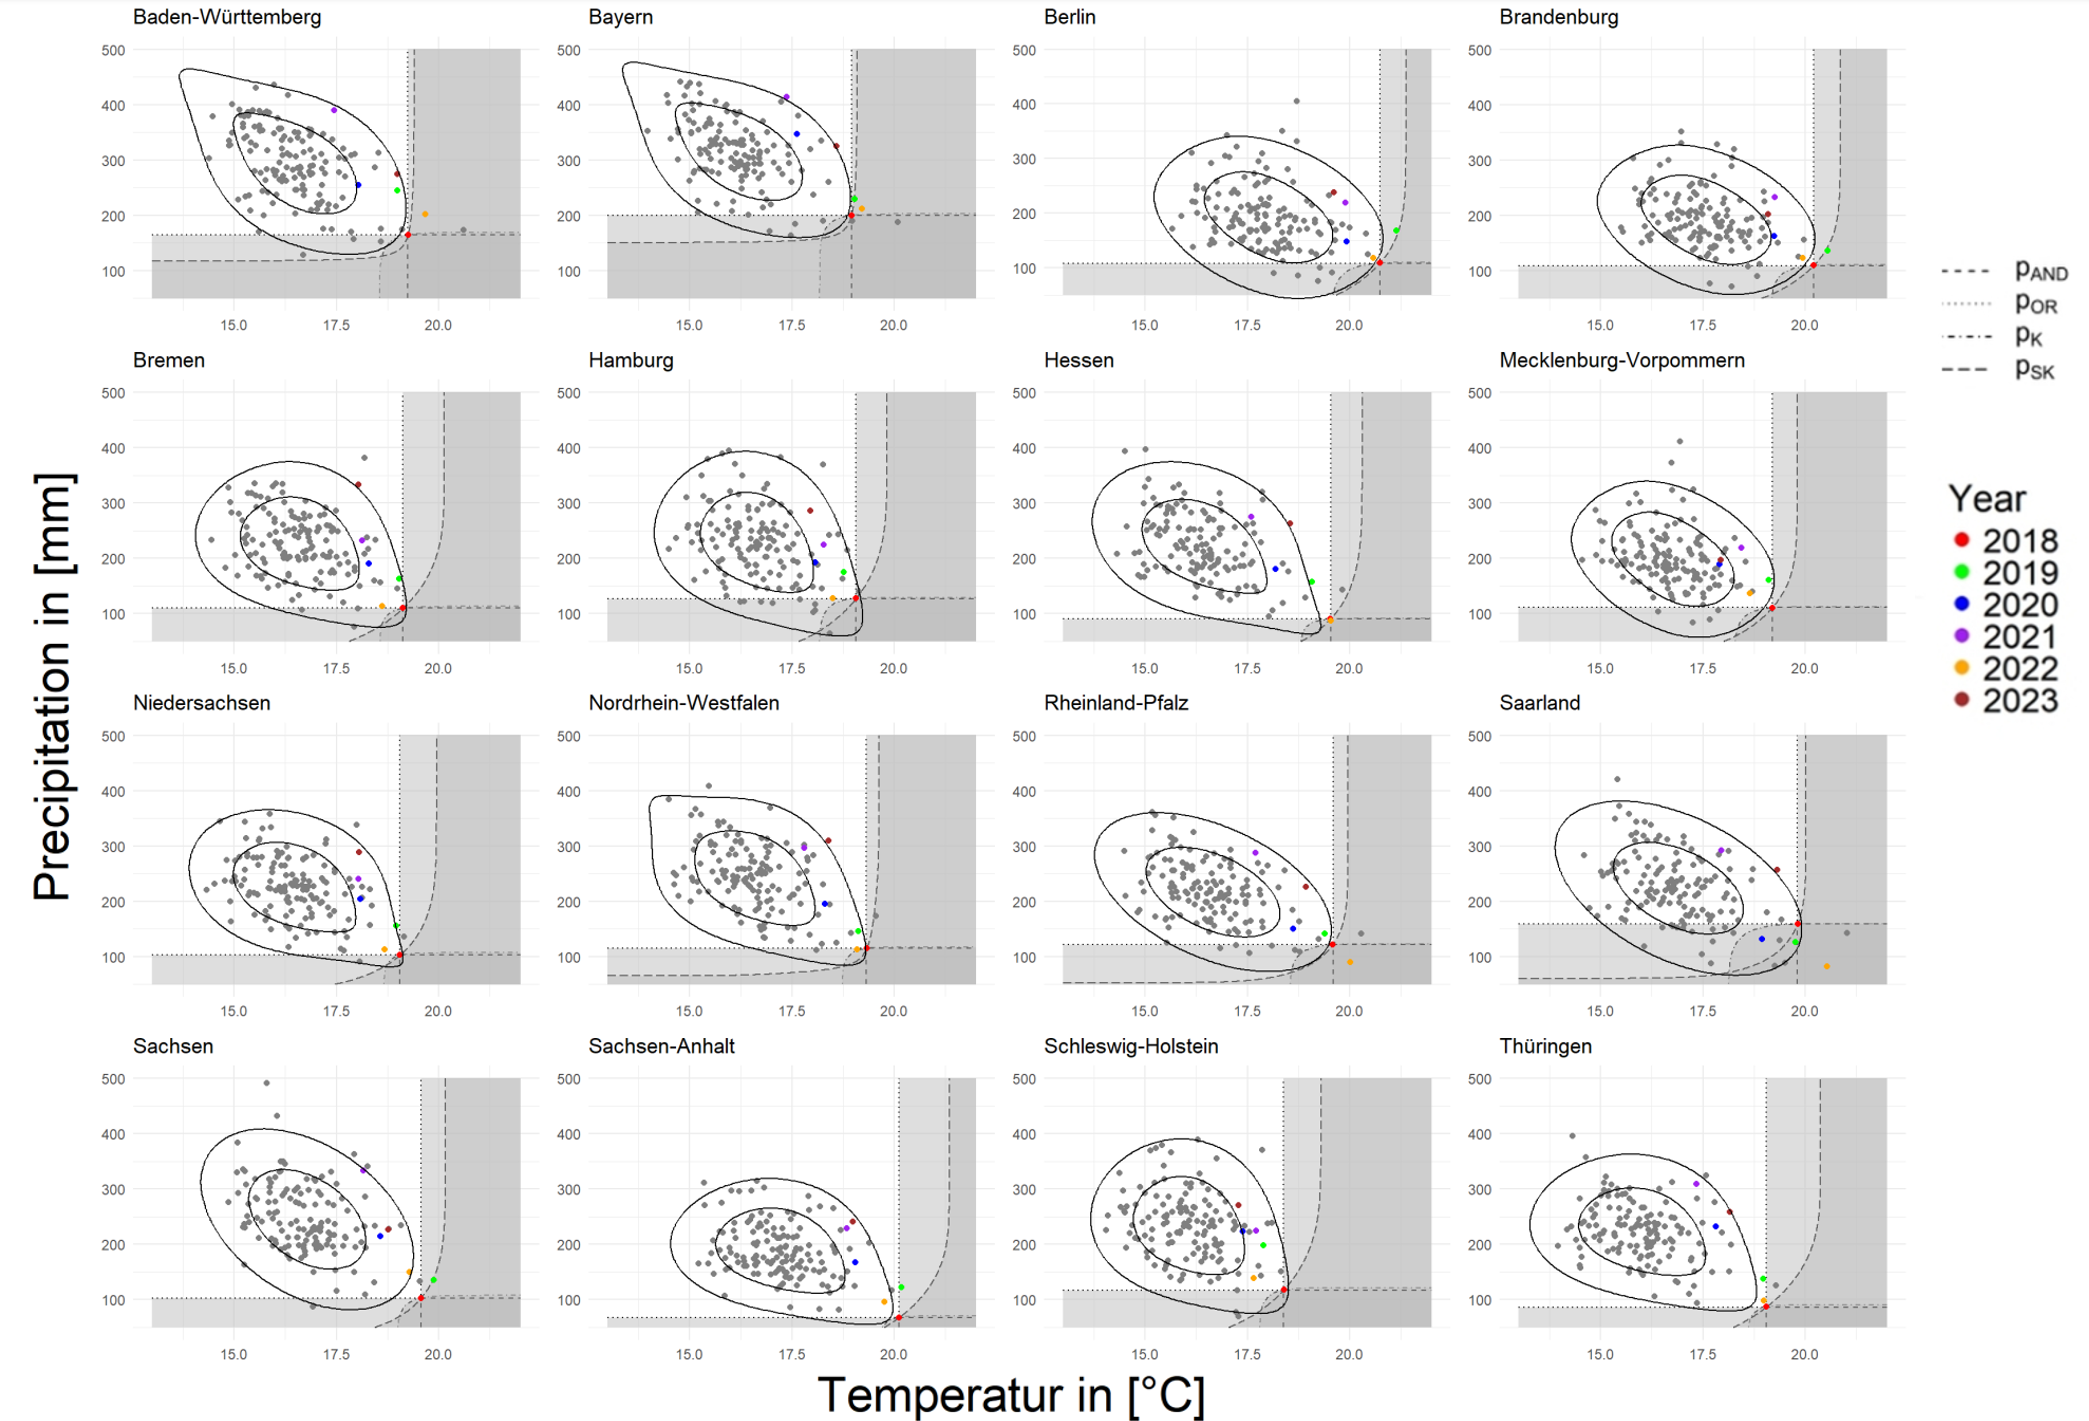
\includegraphics[width=0.8\linewidth]{work/03-compounds/figures/RESULTS/resultJJA} 

}

\caption{Rarity of 2018 for Bundesland from June to August}\label{fig:result5-shiyu}
\end{figure}

\begin{figure}

{\centering 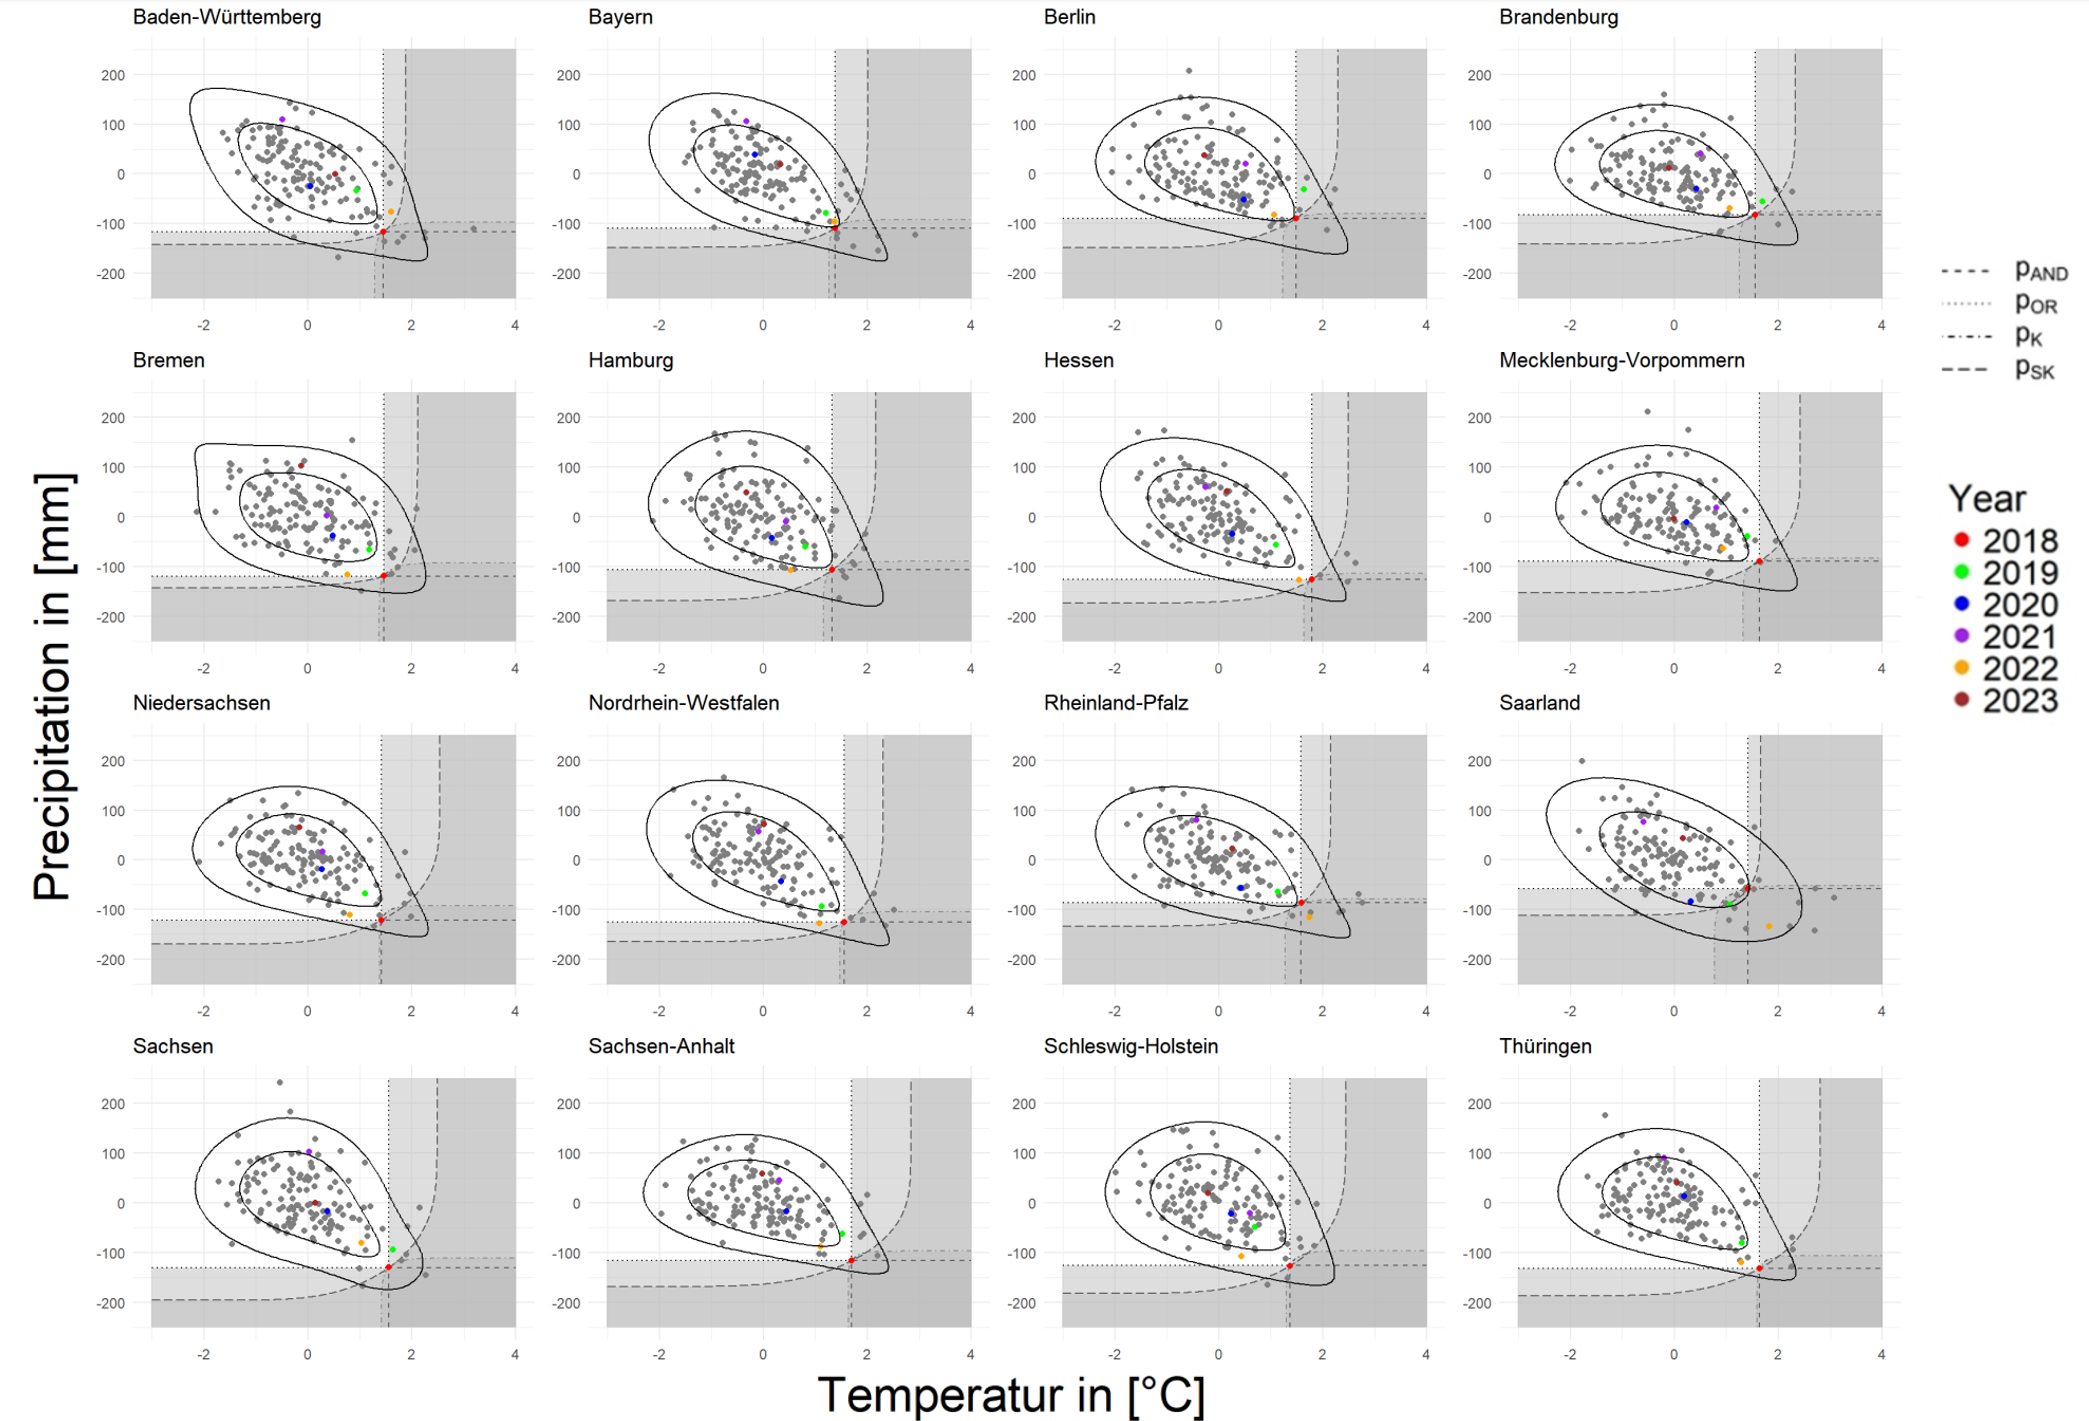
\includegraphics[width=0.8\linewidth]{work/03-compounds/figures/RESULTS/resultJJAA} 

}

\caption{Rarity of 2018 for Bundesland from June to August (Anomalies)}\label{fig:result6-shiyu}
\end{figure}

Turning to Bundesland in Figure \ref{fig:result5-shiyu} and Figure \ref{fig:result6-shiyu}, it seems that many models of the Bundesland cannot capture UTD well over the summer. However, when we use Anomalies the situation immediately improves, with significantly stronger UTD in all areas except Saarland. So let's take a closer look at Saarland, there are more extremes in Saarland in the summer compared to March to November, but it may be that the number of extremes is just too high, leading instead to the fact that in the hottest and driest regions, there is still a very unfocussed distribution of data. In contrast, Sachensen Anhalt, although the extremes are still less, are tightly distributed in the lower right corner, favouring the finding of stronger UTD.

\section{Prediction}\label{prediction}

We also make a prediction to see if a hot and dry climate like 2018 will continue to happen in the future, here we first fit Copula with Anomalies data and then predict the final temperature and precipitation data through the model in 4.5.2. For each of these sets we generate 10,000 sets of data. Due to global Warming is the trend of climate change nowadays, so we use use 5 sets of GMT increasing from 0, which are 0, 1, 1.5, 2, and 3. And the red dots in the graph still represent the data of 2018.

\begin{figure}

{\centering 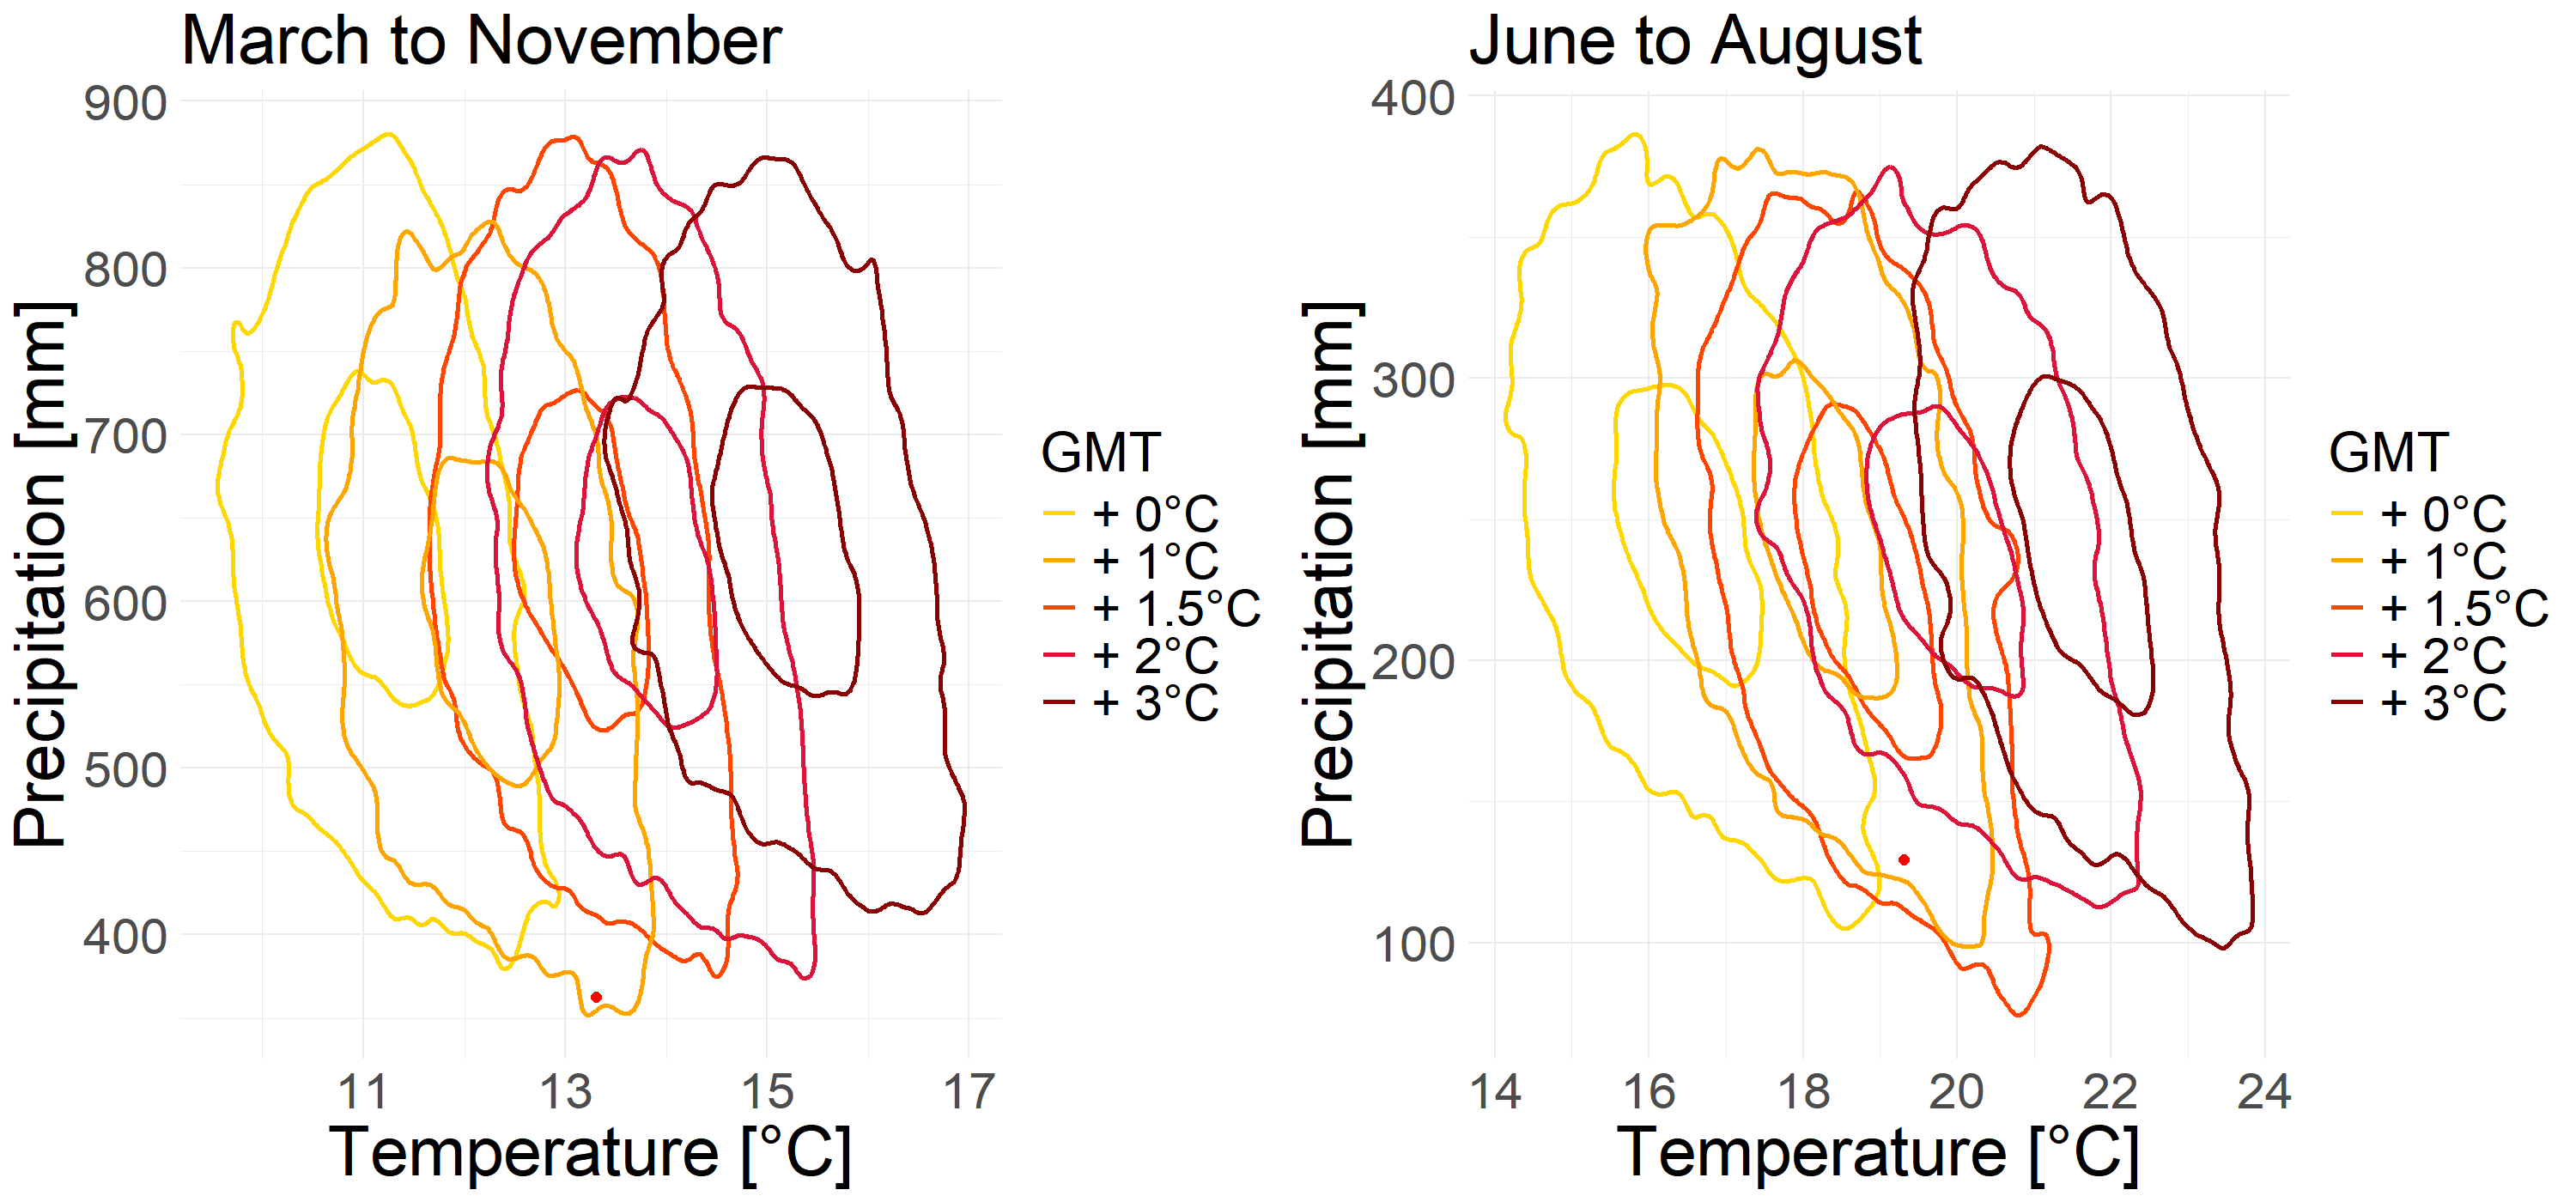
\includegraphics[width=0.8\linewidth]{work/03-compounds/figures/GMT/predictionall} 

}

\caption{Prediction for whole Germany}\label{fig:prediction1-shiyu}
\end{figure}

We can see in Figure \ref{fig:prediction1-shiyu} that for the months of March to November the dry and hot situation is actually unlikely to occur. These contour lines show an overall upward trend, which indicates that in the warmer temperatures at the same time precipitation will actually rise, so the two extremes will not happen at the same time. But for June to August the situation changes completely, while the weather becomes hot, the precipitation also shows a downward trend, so for the summer, the two extremes are likely to occur together.

\begin{figure}

{\centering 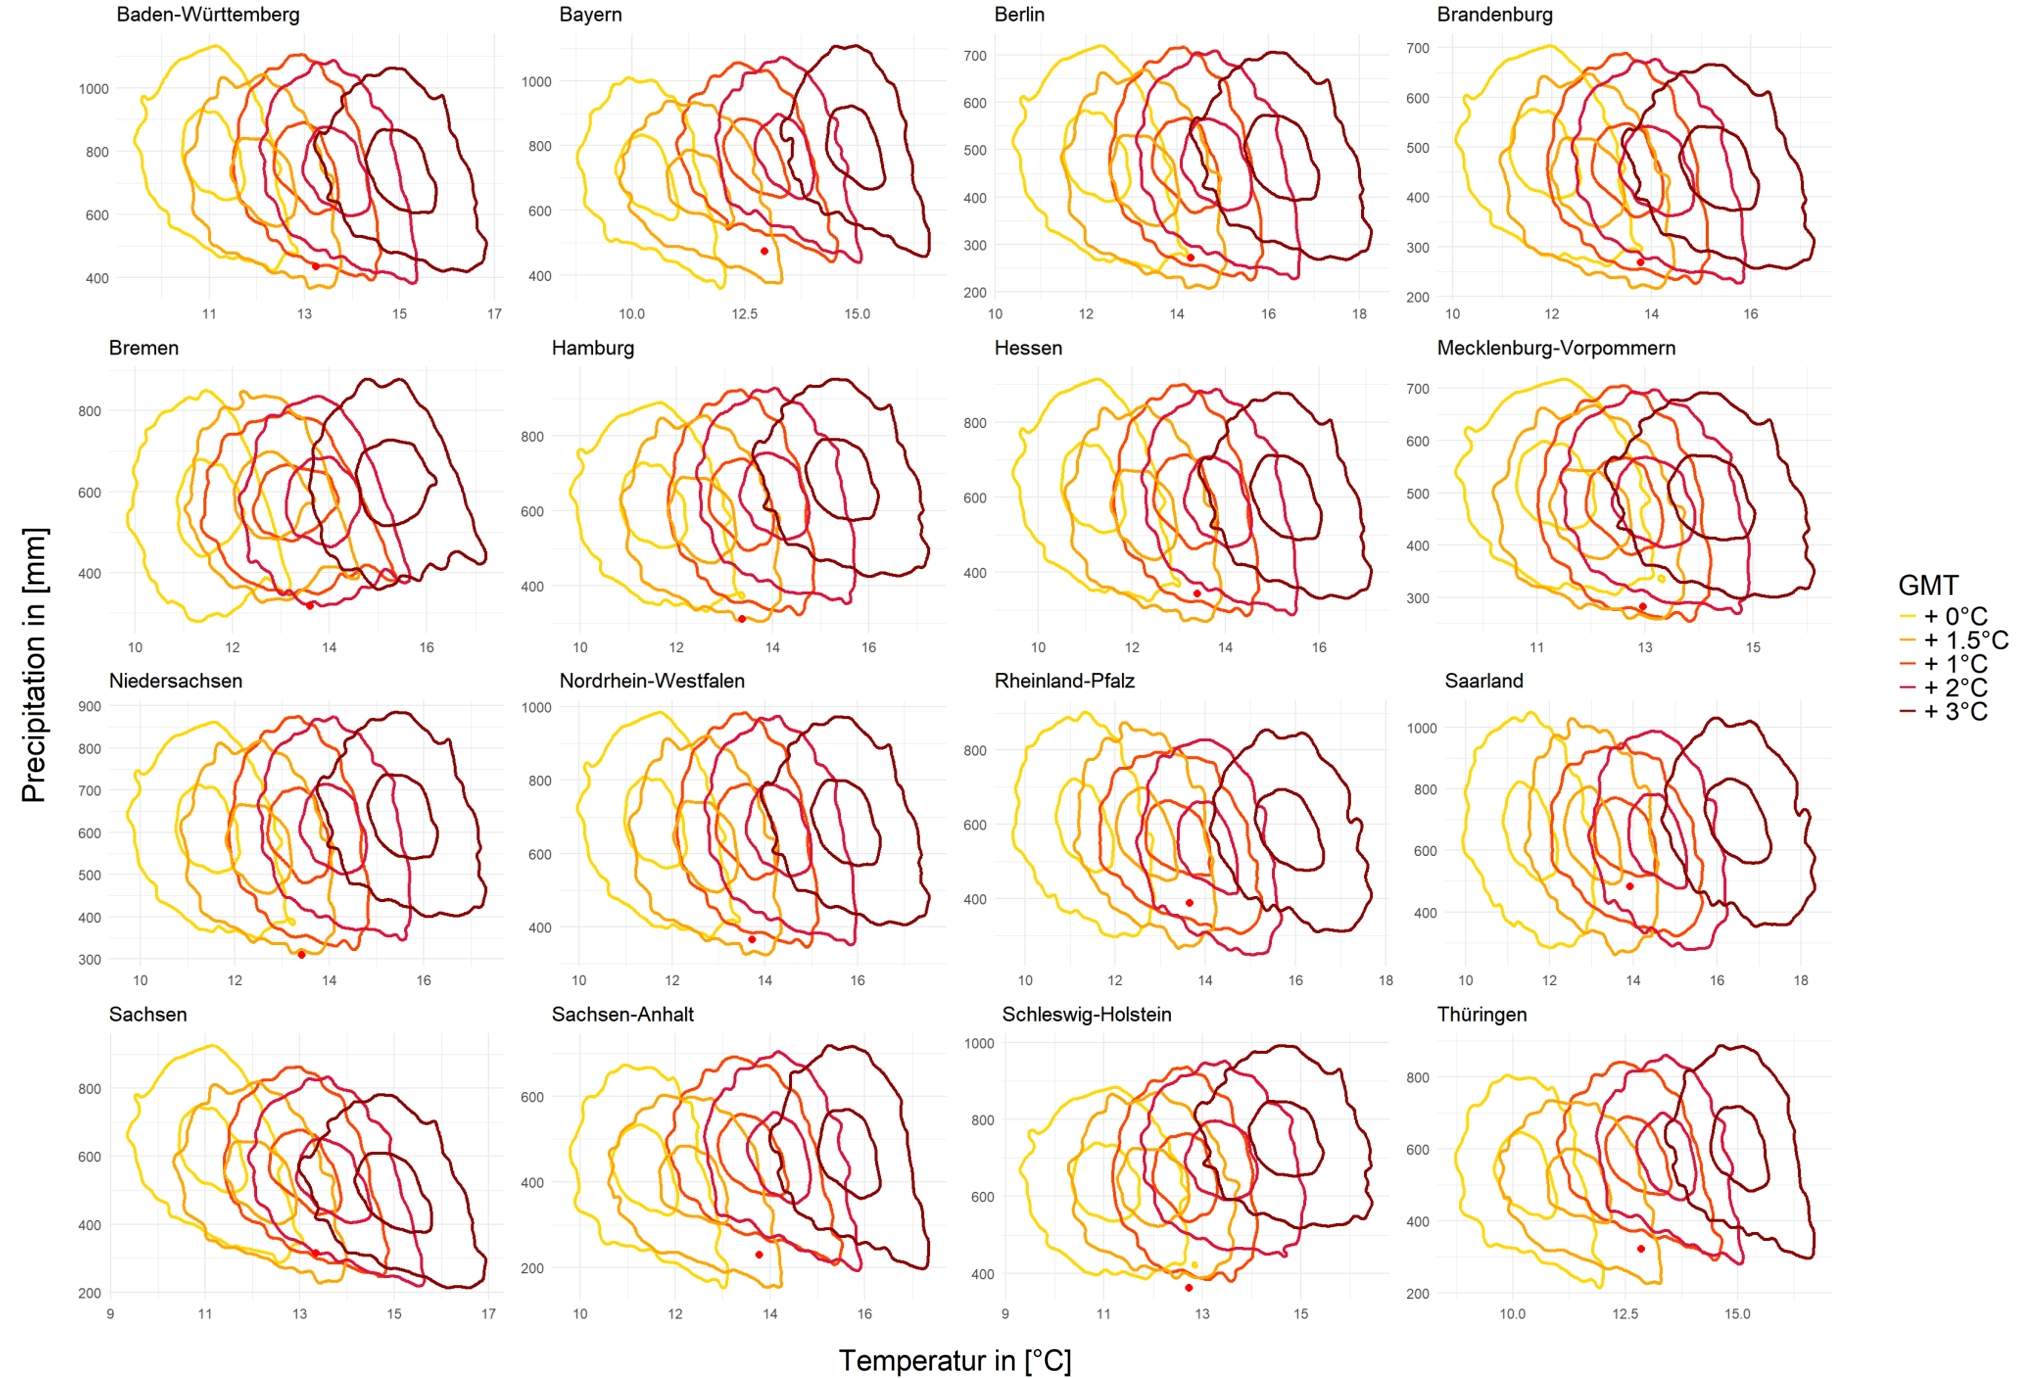
\includegraphics[width=0.8\linewidth]{work/03-compounds/figures/GMT/predictbundeslandMtoN} 

}

\caption{Prediction for Bundesland from March to November}\label{fig:prediction2-shiyu}
\end{figure}

\begin{figure}

{\centering 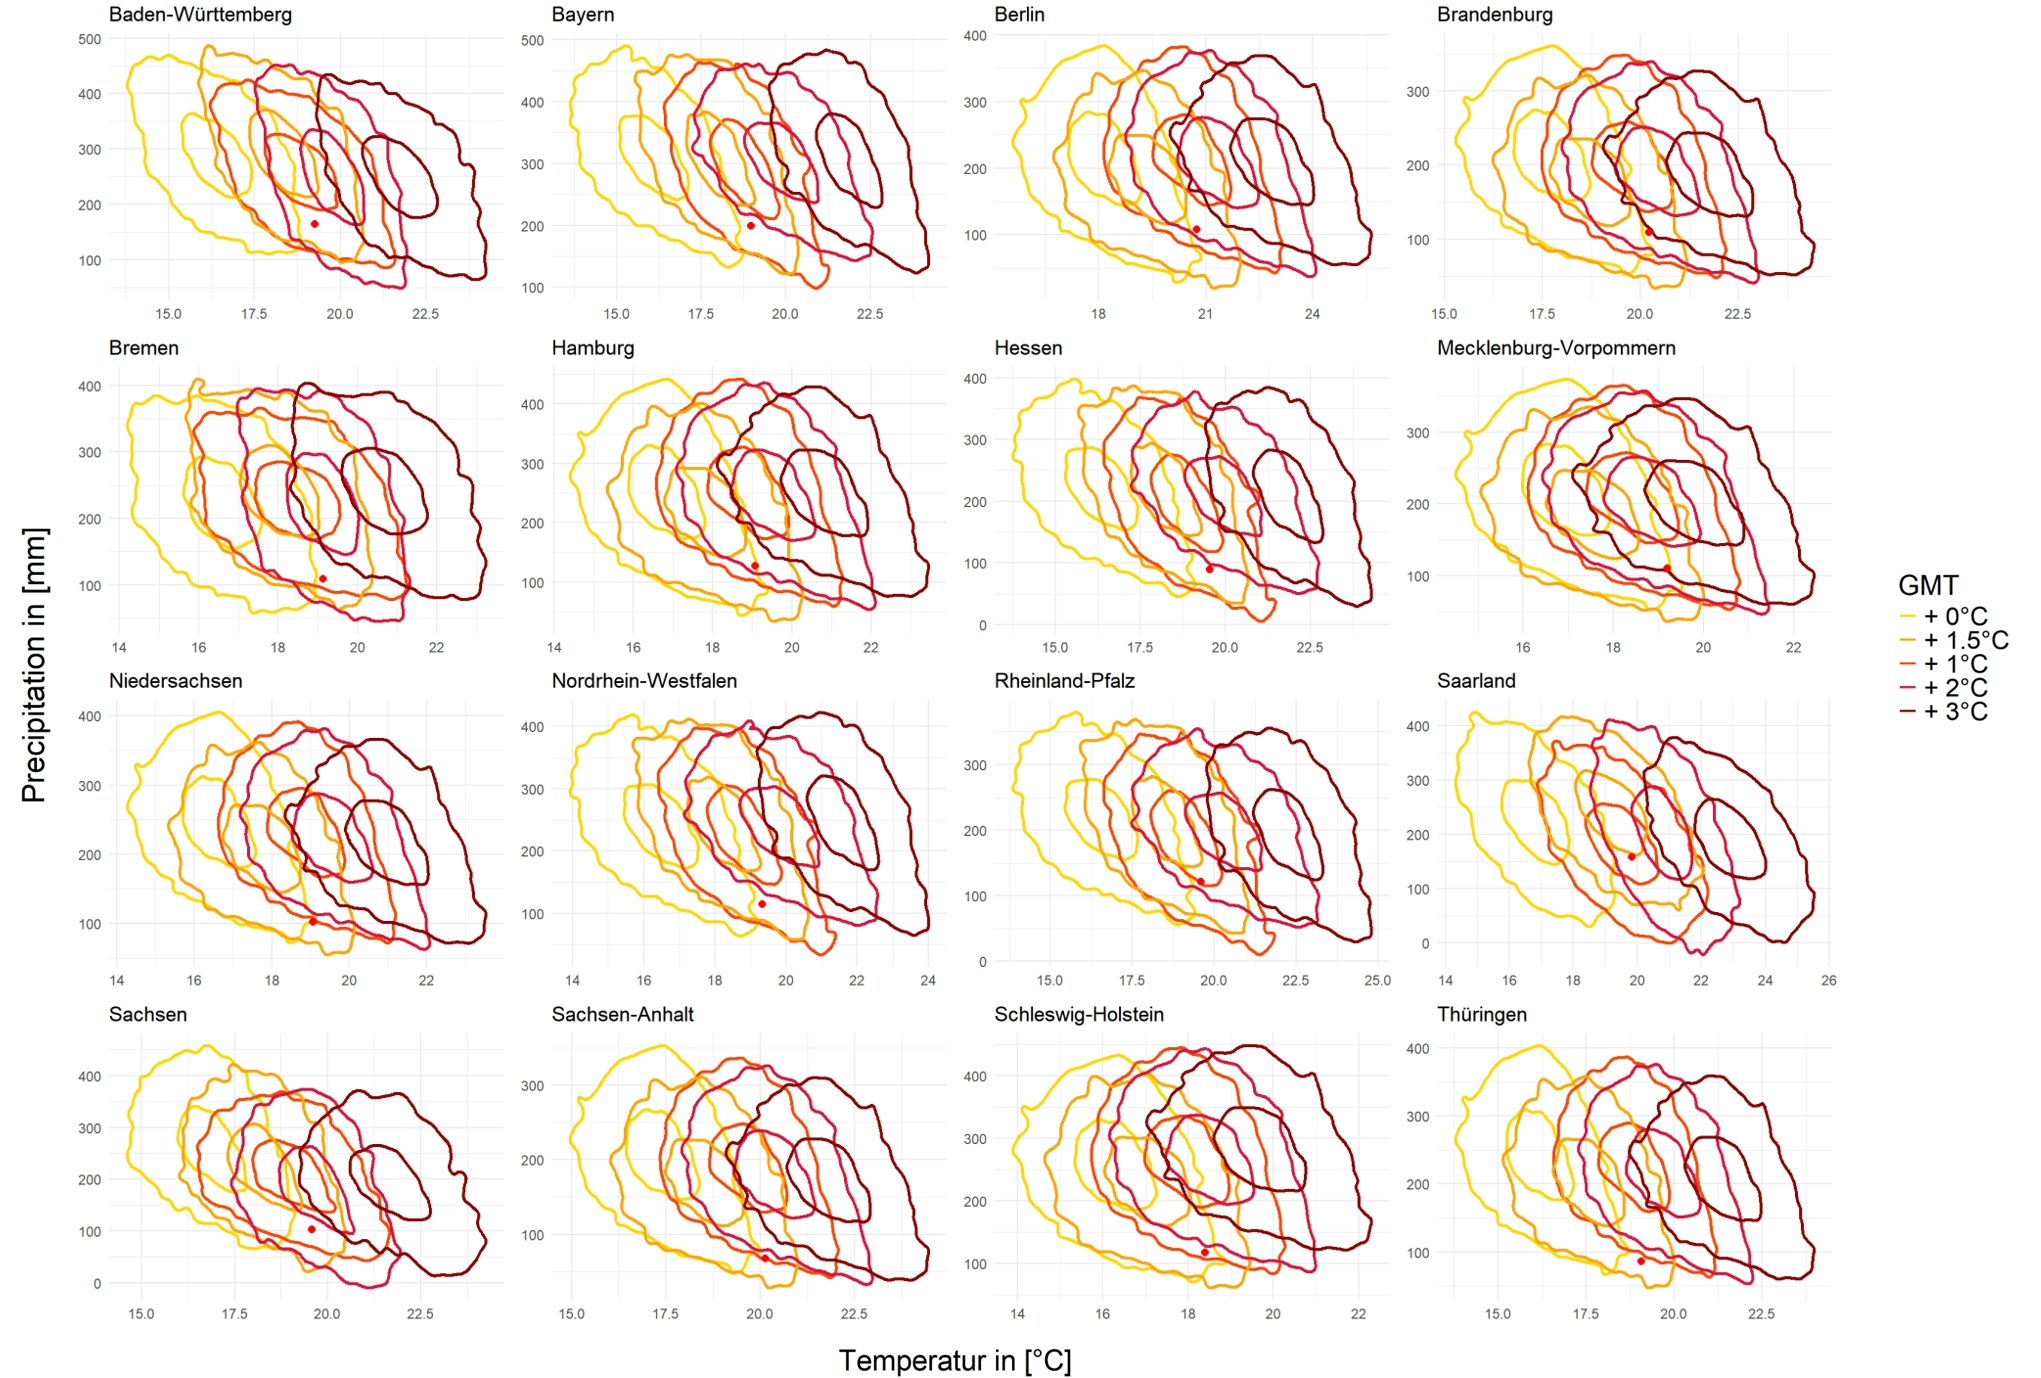
\includegraphics[width=0.8\linewidth]{work/03-compounds/figures/GMT/predictbundeslandJJA} 

}

\caption{Prediction for Bundesland from March to November}\label{fig:prediction3-shiyu}
\end{figure}

And in Figure \ref{fig:prediction2-shiyu} and Figure \ref{fig:prediction3-shiyu} for the bundesland the general trend is the same, in the simulation from March to November only the two Bundesland of Baden and Sachensen show a trend that precipitation also decreases when the temperature increases, the others tend to have more precipitation. For the months of June to August too, most of the Bundesland shows the same trend as the whole of Germany, only Schleswig shows the opposite trend, i.e.~more precipitation. But there are some Bundesland where the precipitation doesn't seem to have changed significantly such as Bremen, Harmburg and so on.

\section{Conclusion}\label{conclusion-1}

There are many types of Copula models, each capturing different features of the data. The selection of a model needs to capture as many features of the data as possible while preventing overfitting. In this study, we use the ``BiCopSelect()'' function and its default criteria AIC to do model selection.

A positive Upper Tail Dependence between temperature and negative precipitation was found both in March to November and June to August in whole Germany. However, when we look at Bundesland, there are many different situations that occur; some Bundesland consistently show high values of UTD, such as Sachsen-Anhalt and Sachsen, and some Bundesland's values of UTD are greatly reduced by the use of fitted marginal distributions, such as Bayern and Hessen. Introducing GMT and removing the effect of global temperature changes on temperature and humidity changes in Germany can reduce the lowering of UTD values by fitting marginal distributions, which is valid for the German data as a whole and many Bundesland, but there are exceptions.

If we consider only the actual temperatures and precipitation, 2018 was the hottest and driest year in Germany since 1881, and in almost all Bundesland states as well. The situation changes if the influences of global temperature changes are excluded. This is not only true for 2018, but also for all the hot years in recent years, which suggests that all regions of Germany have been affected by the global heat in recent years in no small way.

Hot and dry climates like 2018 in March to November will be difficult to come in the future in Germany, even though the global climate may continue to warm, but at the same time precipitation will increase. But if we only look at the summer months, similar situations may occur frequently in Germany. This conclusion also stands for most of Bundesland, but not all of them. It is worth noting that this prediction is very dependent on the relationship between GMT and the variables.

\chapter{Asymmetric bivariate copulas for compounds}\label{ac}

\emph{Author: Claudia Rettenbeck}

\emph{Supervisor: Henri Funk}

\section{Introduction}\label{intro}

There are different definitions of compound events. In this chapter (i.e.~chapter \ref{ac}), a compound event is defined as an extreme event, which is caused by at least two climate variables (e.g.~hydrological variables such as river discharge). Thus, the question of how to model the interplay of several climate variables by means of their multivariate distribution arises. Answering this question lays the basis for modelling compound events, which can, but don't have to, arise from this interplay. After having briefly presented the definition of \(d\)-variate copulas in section \ref{defcop}, this chapter focuses on the interplay of \emph{two} random variables. One approach for modelling multivariate cumulative distribution functions is based on copulas. According to Sklar's theorem, the joint cumulative distribution function of two univariate random variables can be modelled by combining its marginals with a copula (see section \ref{skl} for details). As \citet{genest2007} state, an appropriate model for the dependence structure, which is determined by the copula, can therefore be selected independently from the choice of the marginals, which is advantageous in modelling. Since in this chapter, the focus is on modelling the interplay of two random variables by means of their multivariate distribution via the copula approach, it is possible to further narrow the focus to modelling the dependence structure of these random variables, which will be done in the following. In particular, this chapter concentrates on a specific type of dependence, namely asymmetric dependence. This is relevant for climate research since there are climate variables whose dependence structure is characterized by asymmetry, i.e.~the corresponding random variables are asymmetrically dependent (see section \ref{asymVsSym} for details). For instance, the sections \ref{asymVsSym} and \ref{exAppl} show that the monthly average flow rates (flow rates measure river discharge) of the rivers Inn and Danube can be considered asymmetrically dependent (where the data set presented in the sections \ref{asymVsSym} and \ref{exAppl} is used to draw this conclusion). Thus, when modelling the dependence structure of two climate variables, the assumption of symmetry, which is made when using most classical copulas (see \citet{genest2013}, p.~92), might be too restrictive. Therefore, the goal of this chapter is to lay the theoretical foundation for recognizing and modelling asymmetric dependence between two random variables. There are several approaches for modelling this kind of dependence structure by means of copulas. Due to its scope, this chapter focuses on Archimax copulas as modelling approach, but the interested reader may be referred to chapter 5.4 in \citet{genest2013} for an overview of modelling approaches based on bivariate copulas. Moreover, following a large part of the relevant literature, from section \ref{asymVsSym} onwards, the focus lies on the asymmetric dependence of \emph{continuous} random variables.

While theoretically, a compound event could arise from non-extreme events, climate research often defines compound events via the interplay of extreme events. Thus, while this chapter lays the theoretical foundation for modelling compound events defined according to a broader definition, chapter \ref{ce} presents a stricter version of this definition, which is often used in climate research.

The remainder of this chapter proceeds as follows: Section \ref{backgrcop} provides theoretical background on copulas in general, where also the distinction between symmetric and asymmetric copulas is established. Section \ref{backgrmeas} covers theoretical background on measures of asymmetry in a copula and presents an application of a selection of these asymmetry measures to hydrological data. Section \ref{archi} covers Archimax copulas. Specifically, it defines Archimax copulas, presents well-known special cases of these copulas and explains their asymmetry property. The asymmetry property is not the only relevant property of Archimax copulas (for instance, the fact that an Archimax copula can be constructed with a predetermined extreme value attractor (see \citet{caperaa2000} for details) represents another property, which might be interesting in the context of the climate crisis). Due to the scope of this chapter however, the focus is on the property most relevant to it, i.e.~the asymmetry property. Finally, section \ref{concl} concludes.

\section{Theoretical background on copulas}\label{backgrcop}

\subsection{Definition of d-variate copulas and the special case of bivariate copulas}\label{defcop}

Following \citet{durante2016} (p.~10), copulas can be defined as follows: A \(d\)-dimensional copula \(C\), i.e.~a \(d\)-variate copula, is a \(d\)-dimensional cumulative distribution function concentrated on \([0,1]^d\) with univariate marginals which are uniformly distributed on \([0,1]\), where \(d \geq 2\). Thus, as stated by \citet{durante2016} (p.~10), \(C\) assumes values on \(\mathbb{R}^d\). However, in the literature, \(C\) is frequently defined as a function with domain \([0,1]^d\) and range \([0,1]\), such that \(C\) can be described by \(C: [0,1]^d \to [0,1]\) (see e.g. \citet{durante2010a} and \citet{klement2006}). According to \citet{durante2016} (p.~10), this can be attributed to the fact that \(C\) concentrates the probability distribution on \([0,1]^d\) and therefore the values \(C\) assumes on \(\mathbb{R}^d \setminus [0,1]^d\) are usually not specified.

\citet{durante2016} (p.11) further remark that a random vector \(\mathbf{U}\) (defined on a suitable probability space) corresponds to each copula \(C\) such that the joint cumulative distribution function of \(\mathbf{U}\) is \(C\).

The previous paragraph defines copulas based on their probabilistic interpretation. According to \citet{durante2016} (p.~14), copulas can also be defined in terms of their analytical properties, where the probabilistic and the analytical definition are equivalent:

A function \(C: [0,1]^d \to [0,1]\) is a \(d\)-variate copula if and only if the following holds:

\begin{enumerate}
\def\labelenumi{\roman{enumi})}
\item
  \(C\) is \(d\)-increasing,
\item
  \(C(u_1, \ldots,u_d) = 0\) if \(u_k = 0\) for at least one \(u_k \in \{u_1, \ldots, u_d\}\),
\item
  \(C(1, \ldots, 1, u_k, 1, \ldots, 1) = u_k\), where the left-hand side of the equation means that all arguments equal 1 except possibly for the \(k\)th one, which can assume any value in \([0,1]\).
\end{enumerate}

\citet{durante2016} (p.~14) point out that ii) and iii) are called boundary conditions, where ii) means that \(C\) is grounded (also named anchored) and iii) shows that \(C\) has univariate marginals which are uniform on \([0,1]\).

Since this chapter focuses in the following on bivariate copulas, the expression \(d\)-increasing is not explained in full generality here. Instead an explanation will be provided for the special case of \(d=2\) in the subsequent paragraph. For a more general explanation, see \citet{durante2016} (p.7).

For \(d=2\), the definition above can be translated to (see \citet{durante2016}, p.15 as well as \citet{nelsen2006}, p.~8 and p.~10): A function \(C: [0,1]^2 \to [0,1]\) is a \(2\)-variate copula if and only if the following holds:

\begin{enumerate}
\def\labelenumi{\roman{enumi})}
\item
  \(C\) is \(2\)-increasing, meaning that for all \(a_1, a_2, b_1, b_2 \in [0,1]\), where \(a_1 \leq a_2\) and \(b_1 \leq b_2\), it holds that:
  \(C(a_1, b_1) - C(a_1, b_2) - C(a_2, b_1) + C(a_2, b_2) \geq 0\),
\item
  \(C(0,v) = C(u,0) = 0 \quad \forall u,v \in [0,1]\),
\item
  \(C(1,v) = v\) and \(C(u,1) = u \quad \forall u,v \in [0,1]\).
\end{enumerate}

Note that the names \(2\)-variate copula and bivariate copula are used as synonyms in this chapter.

\subsection{Sklar's theorem and the probability integral transformation}\label{skl}

According to \citet{durante2016} (p.~42), Sklar's theorem states that \emph{any} multivariate cumulative distribution function can be expressed in terms of a copula and its univariate marginals. Specifically, let \((X, Y)\) be a bivariate random vector on a probability space \((\Omega, \mathcal{F}, \mathbb{P})\). Moreover, \(H(x, y) := \mathbb{P}(X \leq x, Y \leq y)\) denotes the joint cumulative distribution function of \((X, Y)\), where \(F(x) = \mathbb{P}(X \leq x)\) and \(G(y) = \mathbb{P}(Y \leq y)\) represent the marginals of \(H\). Then, there exists a bivariate copula \(C = C_{X,Y}\) such that it holds that

\begin{equation}
H(x,y) = C(F(x), G(y)) \quad \forall (x, y) \in \mathbb{R}^2,
\label{eq:sklar}
\end{equation}

where the copula \(C\) is unique, if the marginals \(F\) and \(G\) are continuous.

Note that Sklar's theorem can be generalized to \(d-\)variate copulas easily, where \(d > 2\) (see \citet{durante2016}, p.42 for details), but since this chapter focuses on bivariate copulas, also the version of Sklar's theorem presented here is described for the bivariate case.

For the case of continuos marginals, on which this chapter focuses from section \ref{asymVsSym} onwards, the probability integral transformation plays an important role in understanding Sklar's theorem. Let \(\tilde{X}\) be a random variable on \((\Omega, \mathcal{F}, \mathbb{P})\) with continuous cumulative distribution function \(\tilde{F}\). Then, \(\tilde{F} \circ \tilde{X}\) is called the probability integral transformation and it can be shown that \(\tilde{F} \circ \tilde{X}\) is uniformly distributed on \([0,1]\) (see \citet{durante2016}, pp.~5-6). As \citet{durante2016} (p.~6) note, this means that transforming a random variable by its continuous cumulative distribution function always leads to a random variable that follows the standard uniform distbribution, whereas transforming each component of a random vector by its continuous univariate cumulative distribution function can result in multivariate distributions that differ from the multivariate standard uniform distribution. This can be seen from the proof of equation \eqref{eq:sklar} given in \citet{durante2016} (p.~43) for continuous marginals \(F\) and \(G\), which moreover explains the connection between Sklar's theorem and the probabilistic definition of copulas. The proof requires rewriting \(H(x,y)\) for all \((x, y) \in \mathbb{R}^2\) as follows:

\begin{equation*}
\begin{split}
H(x,y) 
&= \mathbb{P}(X \leq x, Y \leq y) \\
&= \mathbb{P}(F(X) \leq F(x), G(Y) \leq G(y)) \\
&= \mathbb{P}(U \leq F(x), V \leq G(y)),
\end{split}
\end{equation*}

where \(U := F(X)\) and \(V := G(Y)\).
It can be seen from the description of the probability integral transformation above that \(U\) and \(V\) are uniformly distributed on \([0,1]\). As a consequence, the cumulative distribution function of \((U,V)\) has uniform univariate marginals on \([0,1]\), from which it follows that this cumulative distribution function is a copula (see probabilistic definition in section \ref{defcop}). Therefore, \(\mathbb{P}(U \leq F(x), V \leq G(y))\) can be written as \(C(F(x), G(y))\) (recall that \(C\) denotes a copula). Thus, it has been shown that \(H(x,y)=C(F(x), G(y))\).

If \(H\) is absolutely continuous, then the density \(h\) corresponding to \(H\) can be written in terms of the density \(c\) of the copula \(C\). Specifically, \(h\) is given for almost all \((x,y) \in \mathbb{R}^2\) by

\begin{equation}
h(x, y)=c(F(x), G(y)) \cdot f(x) \cdot g(y),
\label{eq:sklardens}
\end{equation}

where \(F\) and \(G\) are the univariate marginals (as above) with the corresponding densities being denoted by \(f\) and \(g\), respectively (see \citet{durante2016}, p.~42).

\subsection{Distinction between symmetric and asymmetric copulas}\label{asymVsSym}

There are different forms of symmetry. Among them are exchangeability, radial symmetry and joint symmetry, where radial symmetry is also called reflection symmetry (see \citet{durante2016}, pp.~30-33). In line with that, \citet{genest2013} (p.~92) note that in the copula literature, the term symmetry can refer to both exchangeability and radial symmetry. However, following the majority of the relevant literature on Archimax copulas reviewed, this chapter defines a copula as symmetric if and only if it is exchangeable.

According to \citet{durante2016} (pp.~30-31), it can be shown that when the cumulative distribution function \(C\) of the random vector \((U,V)\) on a probability space \((\Omega, \mathcal{F}, \mathbb{P})\) is a copula, also the cumulative distribution function \(\tilde{C}\) of \((V,U)\) is a copula. Then, the bivariate copula \(C\) is defined as being exchangeable if

\begin{equation}
C=\tilde{C}.
\label{eq:defsymmgen}
\end{equation}

Note that the definition of exchangeability presented above can be generalized to \(d\)-variate copulas. This generalization is based on the concept of a symmetry and in particular the group of symmetries under the operation of composition. This group includes permutations (see \citet{durante2016}, pp.~30-31 for details), on which the definition above is based.

In the bivariate case, on which this chapter focuses, this translates to a copula being exchangeable if

\begin{equation}
C=C^T,
\label{eq:defsymm}
\end{equation}

where \(C^T(u,v) = C(v,u)\) for all \((u,v) \in [0,1]^2\), i.e.~\(C^T\) is the copula that results from permuting \(C\)'s arguments, and \(C^T\) is also called the transpose of \(C\) (see \citet{durante2016}, p.~31).

Thus, a slightly different form of definition \eqref{eq:defsymm} one often finds in the literature is that a copula is exchangeable if (see e.g. \citet{genest2013}, p.~92)

\begin{equation}
C(u,v)=C(v,u) \quad \forall (u,v) \in [0,1]^2.
\label{eq:defsymm2}
\end{equation}

Asymmetry is then defined via non-symmetry, i.e.~when equation \eqref{eq:defsymm2} is not fullfilled for some \((u,v) \in [0,1]^2\), the copula \(C\) is non-exchangeable, which, as explained above, is defined as being equivalent to asymmetric in this chapter (see \citet{genest2013}, p.~92).

From now on, this chapter (i.e.~chapter \ref{ac}) focuses on continuous random variables, meaning that the random variables, whose univariate cumulative distribution functions enter the copula, are continuous. For instance, for the setting, which has been defined for equation \eqref{eq:sklar}, this means that \(X\) and \(Y\) are restricted to being continuous random variables for the rest of chapter \ref{ac}. Recall from Sklar's theorem that any cumulative distribution function can be expressed in terms of a copula and its univariate marginals and that the copula \(C\) is unique if the marginals \(F\) and \(G\) are continuous. Thus, as described in equation \eqref{eq:sklar}, the cumulative distribution function \(H(x, y)\) can be written as \(H(x, y)=C(F(x), G(y))\) for all \((x, y) \in \mathbb{R}^2\) (for details and definitions see section \ref{skl}). From equation \eqref{eq:defsymm2}, we know that the copula \(C\) is then, symmetric if \(C(F(x), G(y)) = C(G(y), F(x))\) for \emph{all} \((F(x), G(y)) \in [0,1]^2\), i.e.~\(F(x)\) corresponds to \(u\) in equation \eqref{eq:defsymm2}, whereas \(G(y)\) corresponds to \(v\). Then, when this equation is not fullfilled for some \((F(x), G(y)) \in [0,1]^2\), \(C\) is non-exchangeable, i.e.~asymmetric, and the variables \(X\) and \(Y\) are asymmetrically dependent, which usually occurs, when there is a causal relationship between these variables (see \citet{genest2013}, p.~92). As an example, \citet{genest2013} (p.~92) give the monthly average flow rate (in \(m^3/s\)) of the rivers Inn \((X)\) and Danube \((Y)\), which are measured at the stations in Schärding and Nagymaros, respectively. The notation shown in brackets in the previous sentence was chosen since the monthly average flow rate of the rivers Inn and Danube are considered examples for the random variable \(X\) and \(Y\), respectively, which have been introduced above. Note that the flow rate in \(m^3/s\) determined at a given point, measures river discharge, also called river flow, which is the volume of water moving through a river channel (see \citet{copernicus2022} and \citet{copernicus2023}). Moreover, river discharge is considered a climate variable by \citet{copernicus2023}. Thus, \citet{genest2013} investigate the dependence structure of two climate variables, namely (river) discharge of the Inn and (river) discharge of the Danube. The Inn flows into the Danube after it has passed Schärding and afterwards, the Danube passes Nagymaros. For illustration, this situation is depicted in the stylized map shown in figure \ref{fig:stylizedMapClaudia}:



\begin{figure}

{\centering 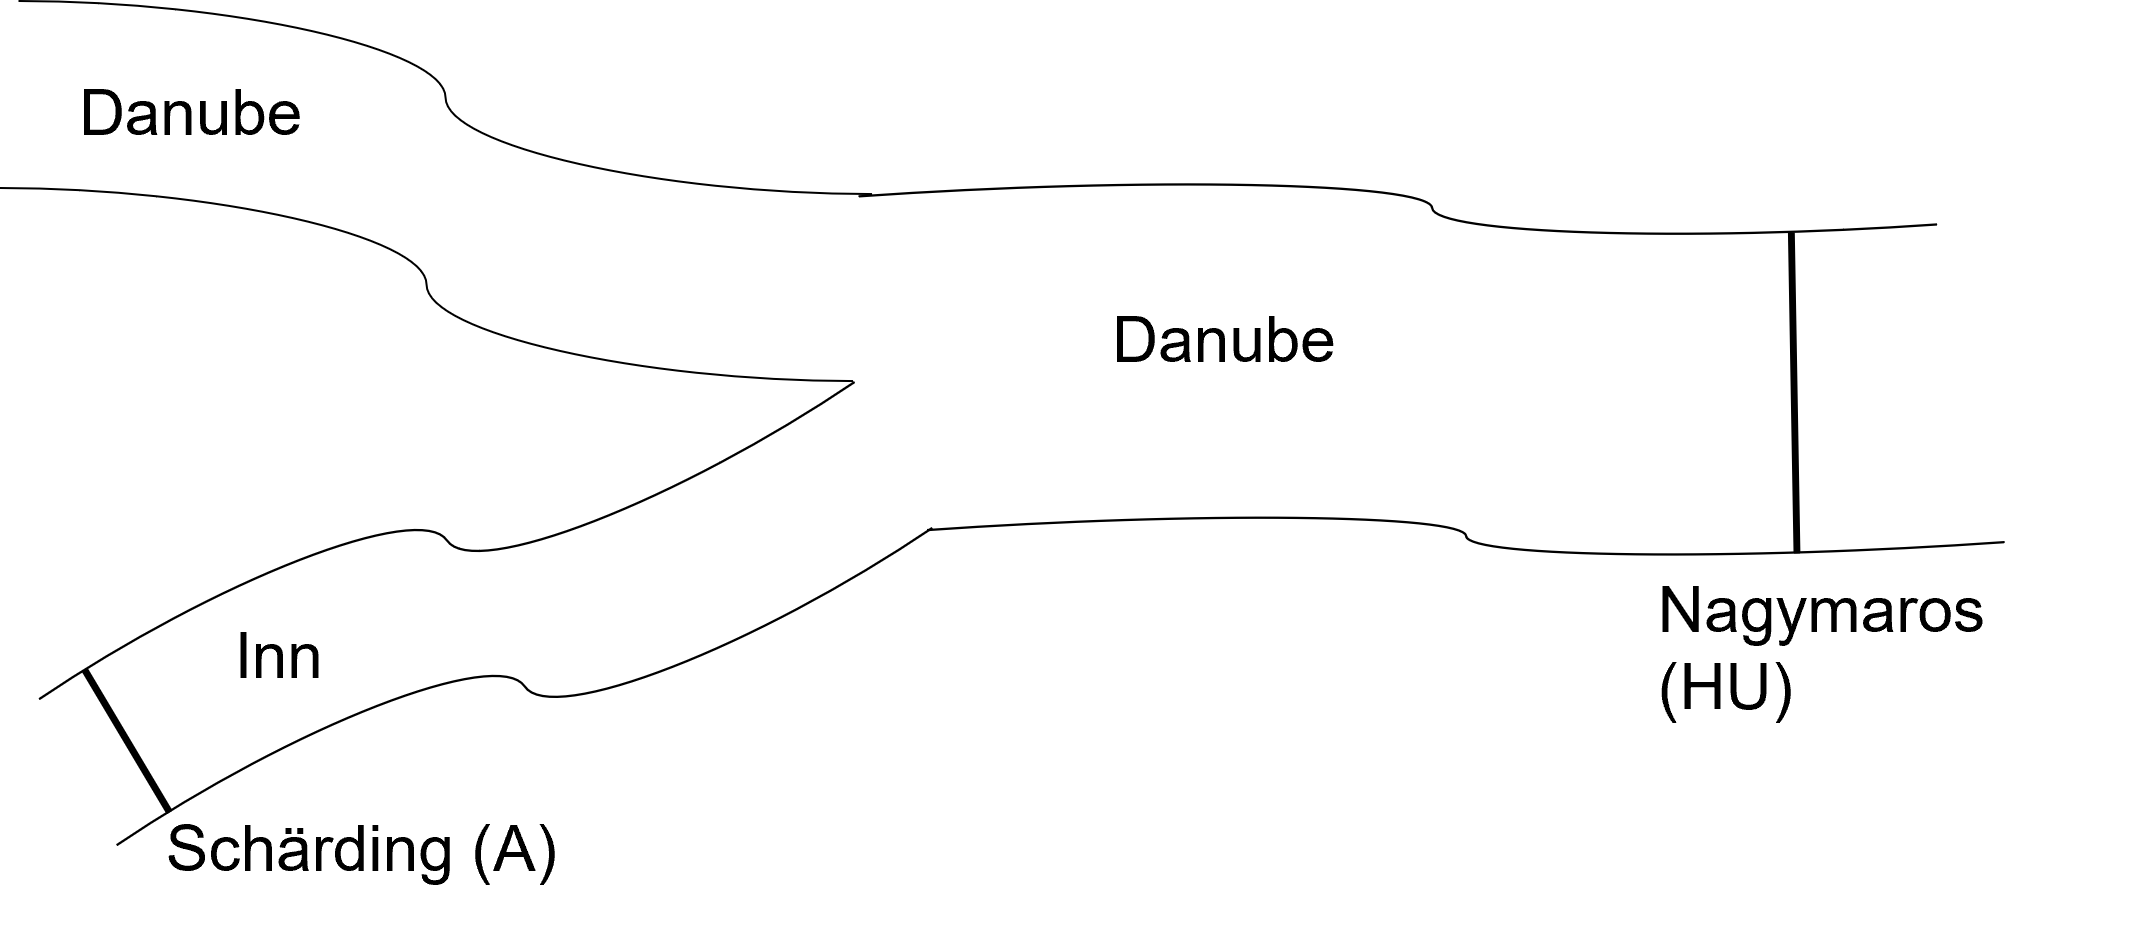
\includegraphics[width=0.7\linewidth]{./work/04-archimax/figures/Map_Inn_Danube_v02} 

}

\caption{Stylized map, which shows the location of the Schärding and Nagymaros measurement stations. Adapted from \citet{genest2013}, p. 92.}\label{fig:stylizedMapClaudia}
\end{figure}

Thus, high discharge of the Inn is likely to cause high discharge of the Danube, but not vice versa, where this circumstance describes a causal relationship. Consequently and as also pointed out by \citet{genest2013} (p.~92), one would expect to observe high discharge of the Danube, when the discharge of the Inn is high, but not necessarily the other way round.

\section{Theoretical background on measures of asymmetry in a copula and their application to hydrological data}\label{backgrmeas}

\subsection{Measures of asymmetry in a copula}\label{measures-of-asymmetry-in-a-copula}

The question arises how to measure the degree of asymmetry in a copula. \citet{durante2010a} introduce measures of asymmetry in an axiomatic way. Specifically, they define the term measure of asymmetry for the class of (bivariate) copulas \(\mathcal{C}\) as a function \(\mu:\mathcal{C} \rightarrow \mathbb{R}^+_0\) that satisfies the following axioms:

\begin{itemize}
\tightlist
\item
  (A1) There exists \(L \in \mathbb{R}^+_0\) such that: \(\mu(C) \leq L \quad \forall C \in \mathcal{C}\),
\item
  (A2) \(\mu(C) = 0\) if and only if \(C = C^T\), i.e.~\(C\) is symmetric,
\item
  (A3) \(\mu(C) = \mu(C^T) \quad \forall C \in \mathcal{C}\),
\item
  (A4) \(\mu(C) = \mu(\check{C}) \quad \forall C \in \mathcal{C}\),
\item
  (A5) \((\mu(C_n))_{n \in \mathbb{N}}\) converges to \(\mu(C)\) if \((C_n)_{n \in \mathbb{N}}\) converges uniformly to \(C\) and if \((C_n)_{n \in \mathbb{N}} \in \mathcal{C}\) and \(C  \in \mathcal{C}\),
\end{itemize}

where \(\check{C}\) is the so-called survival copula of \(C\) with \(\check{C}(u,v) = u + v - 1 + C(1-u, 1-v)\) for all \((u,v) \in [0,1]^2\) (for further details on survival copulas, see \citet{durante2016}, pp.~32-33).

Axiom (A1) ensures that the measure \(\mu(C)\) is bounded which will help interpretation (see below), whereas axiom (A2) makes sure that when the measure \(\mu(C)\) assumes the value zero, it can be concluded that the copula is symmetric (and vice versa). The remaining axioms (A3) to (A5) reflect certain invariance properties of the exchangeability of a random pair, which translates to the symmetry of the corresponding copula if exchangeability is given (see \citet{durante2010a} for details).
\citet{durante2010a} then show that the function \(\mu_p:\mathcal{C}\rightarrow \mathbb{R}^+_0\) is a measure of asymmetry for all \(p \in [1, \infty]\), where for \(p \in [1, \infty)\)

\begin{equation}
\mu_p(C) = \left( \int_0^1 \int_0^1 |C(u, v) - C(v, u)|^p \, du \, dv \right)^{1/p}
\label{eq:asymmeassupgen}
\end{equation}

and for \(p = \infty\)
\begin{equation}
\mu_{\infty}(C) = \max_{(u,v) \in [0,1]^2} |C(u, v) - C(v, u)|.
\label{eq:asymmeassup}
\end{equation}

Moreover, they point out that equation \eqref{eq:asymmeassupgen} and equation \eqref{eq:asymmeassup} describe a large class of asymmetry measures.

Note that the class of asymmetry measures described above has been discussed by \citet{klement2006} and \citet{nelsen2007} before \citet{durante2010a}, but without basing it on axioms.

An alternative measure of asymmetry has been introduced by \citet{genest2013} (pp.~96-97). Its main advantage is that the corresponding estimate can be calculated more easily than in case of \(\mu_p\) for \(p \neq 2\) and \(p \neq \infty\). Since in this chapter, the focus is not on the estimation procedure, this is not explored further. Moreover, other alternative measures can be found in the literature, which were discussed shortly by \citet{genest2013} (p.~94). Following their work however, these measures are not explored further here. More recently, additional measures of asymmetry have been proposed (see e.g. \citet{kamnitui2018}). Since the class of measures described above is relatively large, is based on a broad axiomatic approach, still appears to be relevant in practice (see \citet{lin2020}) and has been studied relatively extensively in the context of Archimax copulas, this class of measures appears to be the most important one for the questions this chapter addresses, wherefore the focus is set accordingly.

\subsection{Bounds for measures of asymmetry in a copula and the resulting possibility for normalization}\label{bounds}

\citet{klement2006} and \citet{nelsen2007} show that \(\frac{1}{3}\) is an upper bound for the asymmetry measure defined by \eqref{eq:asymmeassup}, i.e.~for every copula \(C\) the following inequality holds:

\begin{equation}
\mu_{\infty}(C) \leq \frac{1}{3} =: \eta_\infty.
\label{eq:upboundasyminf}
\end{equation}
Moreover, they show that inequality \eqref{eq:upboundasyminf} holds with equality for some \(C \in \mathcal{C}\).

Also for asymmetry measures defined by equation \eqref{eq:asymmeassupgen}, an upper bound exists for every copula \(C\) (see \citet{durante2010a}). Specifically, for \(p \in [1,\infty)\) it holds that

\begin{equation}
\mu_p(C) \leq \left( \frac{2 \cdot 3^{-p}}{(p+1)(p+2)} \right)^{1/p} =: \eta_p.
\label{eq:upboundasymp}
\end{equation}

\citet{durante2010a} conclude that thus for \(p \in [1,\infty]\), an asymmetry measure \(\mu_p(C)\) can be normalized as follows:

\begin{equation}
\frac{\mu_p(C)}{\eta_p} =: \nu_p(C)
\label{eq:asymmeasnorm}
\end{equation}
and therefore \(\nu_p:\mathcal{C} \rightarrow [0,1]\), i.e the range of \(\nu_p\) is the interval \([0,1]\).

Note however that it is unknown if for \(p \in [1,\infty)\) the corresponding upper bound is attained. It is true that \citet{durante2010a} show that for every measure of asymmetry \(\mu:\mathcal{C} \rightarrow \mathbb{R}^+_0\) there is a copula \(\overset{\circ}{C}_{\mu} \in \mathcal{C}\) and a constant \(L_{\mu} \in \mathbb{R}^+_0\) such that \(\mu(C) \leq L_{\mu}\) for all \(C \in \mathcal{C}\) and \(\mu(\overset{\circ}{C}_{\mu}) = L_{\mu}\), but it is not clear if \(\eta_p = L_{\mu}\) for \(\mu = \mu_p\) and \(p \in [1,\infty)\). Thus, \(\nu_\infty\) takes values in the entire interval \([0,1]\), but for \(p \in [1,\infty)\) it can only be said that \(\nu_p \in [0,1]\) (see \citet{genest2013}, p.~97).

\subsection{Example of an application of a selection of the asymmetry measures described above to hydrological data}\label{exAppl}

\citet{genest2013} (pp.~95-98) use two of the asymmetry measures described above to asses the asymmetry in the dependence of the flow rates of two rivers. Specifically, they use data on monthly average flow rates (in \(m^3/s\)) of the rivers Inn and Danube, which were determined at the Schärding and Nagymaros measurement stations in the period from 1936 to 1991, i.e.~over a period of 55 years (see section \ref{asymVsSym} for an explanation why these two random variables are expected to be asymmetrically dependent). From this data, they obtain 660 values \((u_i, v_i)\), where for each \(i \in \{1,\ldots, n\}\), \((u_i, v_i) = (F_n(x_i), G_n(y_i))\), with \(n\) representing the sample size and \(x_i\) denoting the realization of the \(i\)th monthly average flow rate of the Inn \(X_i\). Analogously, \(y_i\) represents the realization of the \(i\)th monthly average flow rate of the Danube \(Y_i\). Furthermore, \(F_n\) and \(G_n\) denote the marginals of the (rescaled) empirical cumulative distribution function \(H_n\) corresponding to \(H\), where \(H_n\) is calculated from the realizations of the sample \((X_1, Y_1),\ldots,(X_n, Y_n)\) and \(H\) represents, as introduced above, the theoretical joint cumulative distribution function of \((X_i, Y_i)\) for all \(i \in \{1,\ldots, n\}\) with unique copula \(C\). Therefore, for each \(i \in \{1,\ldots, n\}\), \((u_i, v_i) = (F_n(x_i), G_n(y_i))\) can be seen as a pseudo-observation from \(C\). These pseudo-observations are shown in figure \ref{fig:scatterClaudia}, which thus visualizes the dependence structure in the data (see \citet{durante2016}, p.~43).



\begin{figure}

{\centering 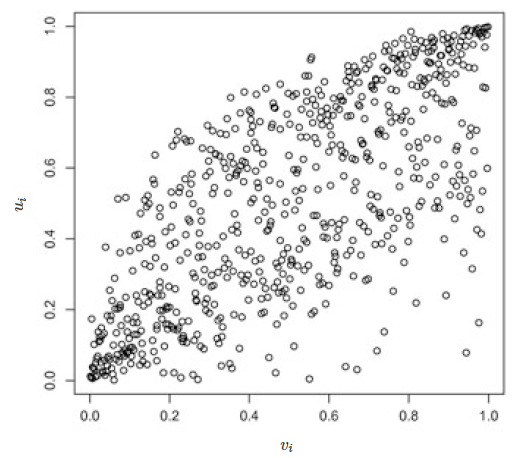
\includegraphics[width=0.6\linewidth]{./work/04-archimax/figures/Plot_Inn_Danube_raw_adjusted_v02} 

}

\caption{Scatter plot of the pseudo-observations \((u_1, v_1) \ldots, (u_n, v_n)\) from \(C\), where \(u_i\) is calculated from data on the Inn and \(v_i\) is obtained from data on the Danube (\(\forall i \in \{1,\ldots, n\}\)). Adapted from \citet{genest2013}, p. 93.}\label{fig:scatterClaudia}
\end{figure}

As can be seen from this figure, the visualization of the dependence structure supports the notion of asymmetry in the dependence between \(X\) and \(Y\), where this conclusion has also been drawn by \citet{genest2013} (p.~92).

Based on the insight that \((u_1, v_1), \ldots, (u_n, v_n)\) can be seen as pseudo-observations from \(C\), \citet{genest2013} (p.~96) calculate the empirical copula \(\hat{C}_n\) as an estimate of \(C\). Then, they use \(\hat{C}_n\) to calculate estimates of \(\mu_2(C)\) and \(\mu_\infty(C)\) (for details on their estimation procedure, see \citet{genest2013}, pp.~95-96). These estimates are then standardized using the upper bounds for the corresponding measure, namely \(\eta_2=1/\sqrt{54}\) and \(\eta_\infty=1/3\). Afterwards, these standardized estimates are used as estimates of \(\nu_2(C)\) and \(\nu_\infty(C)\) as defined by equation \eqref{eq:asymmeasnorm}. This results in

\(\nu_\infty(\hat{C}_n) = 3 \mu_{\infty}(\hat{C}_n) \approx 0.127\)

and

\(\nu_2(\hat{C}_n) = \sqrt{54} \mu_2(\hat{C}_n) \approx 0.083.\)

As explained in section \ref{bounds}, the values \(\nu_\infty\) and \(\nu_2\) assume lie in the interval \([0,1]\). For \(\nu_\infty\) we know additionally that it takes values in the entire interval \([0,1]\). This is not clear for \(\nu_2\), since the bound \(\eta_2\) might not be sharp (see section \ref{bounds} as well as \citet{genest2013}, p.~97), but following the assessment of \citet{genest2013} (p.97) that \(\eta_2\) still is reasonable for standardization in practice, the estimates of both \(\nu_{\infty}(C)\) as well as \(\nu_2(C)\) appear to be relatively small. Since a value of 0 indicates symmetry (see section \ref{backgrmeas}), this does not provide strong support for the notion of asymmetry.
A similar result is obtained when the series is de-trended to avoid the time-invariant dependence measured between the two variables being distorted by serial dependence, which is possible since the data used shows time trends (see \citet{genest2013}, p.~97). Still, the estimates \citet{genest2013} (p.~98) obtain from this approach are relatively small. Specifically, they obtain

\(\nu_\infty(\hat{C}_n) = 3\mu_{\infty}(\hat{C}_n) \approx 0.091\)

and

\(\nu_2(\hat{C}_n) = \sqrt{54} \mu_2(\hat{C}_n) \approx 0.063.\)

Positive dependence supports symmetry in the sense that certain positive dependence properties can induce upper bounds on asymmetry measures which are relatively close to zero (see \citet{genest2013}, p.~95 for details) and \citet{genest2013} (p.~98) find that the two variables investigated here are clearly positively correlated. For instance, the sample value of Kendall's tau as reported by \citet{genest2013} (p.~98) equals approximately 0.525 for the raw data and it assumes a similar value, namely 0.548, for the de-trended data. Thus, the small values of the asymmetry measures reported above might not be entirely surprising. In order to investigate if the estimates reported above are significantly greater than zero, and thus the dependence between the two variables can be considered asymmetric, \citet{genest2013} (pp.~98-101) conduct formal statistical tests for both the raw and the de-trended data. Since the null hypothesis of symmetry was rejected in all cases, approaches to model asymmetry, such as Archimax copulas, should be considered for this example of hydrological data.

\section{Archimax copulas}\label{archi}

\subsection{Definition}\label{definition}

Since Archimax copulas are only symmetric under a condition that will be made precise in section \ref{asymarchi}, they can be used for modelling asymmetric dependence between random variables. Archimax copulas have been introduced by \citet{caperaa2000}. Following \citet{caperaa2000}, \citet{bacigal2011} as well as \citet{durante2010b}, the following bivariate function is a copula and is called Archimax copula:

\begin{equation}
C_{\phi, A}(u, v) = \phi^{[-1]} \left[ (\phi(u) + \phi(v)) A \left( \frac{\phi(u)}{\phi(u) + \phi(v)} \right) \right] \quad \forall (u,v) \in [0,1]^2
\label{eq:archimax}
\end{equation}

with the conventions \(0/0 = \infty/\infty=0\) (see \citet{bacigal2011}) and where

\begin{enumerate}
\def\labelenumi{\roman{enumi})}
\item
  \(A: [0, 1] \rightarrow [1/2, 1]\) is a convex function such that \(\max(t, 1 - t) \leq A(t) \leq 1\) for all \(0 \leq t \leq 1\),
\item
  \(\phi: [0, 1] \rightarrow [0, \infty]\) is a convex, strictly decreasing and continuous function for which it holds that \(\phi(1) = 0\) and with pseudo-inverse
\end{enumerate}

\begin{equation}
\phi^{[-1]}(t) = 
\begin{cases} 
\phi^{-1}(t), & 0 \leq t \leq \phi(0), 
\\0, & otherwise.
\label{eq:pseudoinv}
\end{cases}
\end{equation}

Functions \(A\) as defined in i) are called dependence functions (see \citet{caperaa2000} and \citet{bacigal2011}) or Pickands dependence functions (see \citet{genest2013}, pp.~101-102 and p.~105) and functions \(\phi\) as defined in ii) are called Archimedean generators (see \citet{caperaa2000}) or just generators (see \citet{bacigal2011}).

\subsection{Archimedean and extreme value copulas as special cases of Archimax copulas}\label{special}

There are two special cases of Archimax copulas, namely Archimedean copulas and extreme value copulas (see e.g. \citet{caperaa2000} and \citet{durante2010b}). In the following, it is described under which conditions these special cases arise:

When \(A \equiv 1\), Archimax copulas can be written as

\begin{equation}
C_{\phi, A}(u, v) = C_{\phi}(u, v) = \phi^{[-1]}\left[\phi(u) + \phi(v) \right] \quad \forall (u,v) \in [0,1]^2,
\label{eq:archimedan}
\end{equation}

where the equation above corresponds to a bivariate Archimedean copula as described by \citet{nelsen2006} (pp.~110-112). Note that Archimedean copulas are symmetric (see also \citet{genest2013}, p.~103).

In contrast, for \(\phi(t)=log(1/t)\), an Archimax copula can be written in the general form of a bivariate extreme value copula (see \citet{durante2010b}), i.e.~as

\begin{equation}
C_{\phi, A}(u, v) = C_A(u, v) = \exp\left[ \log(uv) A\left( \frac{\log(u)}{\log(uv)} \right) \right] \quad \forall (u, v) \in (0,1)^2.
\label{eq:extreme}
\end{equation}

Extreme value copulas are only symmetric under a condition, which will be made precise in section \ref{asymarchi}. Note that this is in contrast to Archimedean copulas.

Well-known examples of extreme value copulas are the independence copula \(\Pi(u, v) = u \cdot v\) as well as the comonotonicity copula \(M(u, v) = \min\{u, v\}\) (see \citet{durante2010b}). The dependence structure the independence copula induces corresponds to the one its name suggests (see \citet{durante2016}, p.~63 as well as p.11 for details). Also the comonotonicity copula obtains its name from the dependence structure it induces, where comonotonicity is the strongest concept of positive dependence (see \citet{durante2016}, pp.~64-65 as well as p.11 for details).

\subsection{Asymmetry}\label{asymarchi}

While the majority of classical copulas is symmetric (see \citet{genest2013}, p.~92), according to \citet{bacigal2011}, an Archimax copula \(C_{\phi, A}\) as defined in \eqref{eq:archimax} is symmetric if and only if

\begin{equation}
A(t) = A(1-t) \quad \forall t \in [0,1].
\label{eq:archasymcond}
\end{equation}

Thus, when \(A(t) \neq A(1-t)\) for some \(t \in [0,1]\), Archimax copulas are asymmetric. Note that the same holds for the special case of extreme value copulas (see also \citet{genest2013}, p.~102).

However, the degree of asymmetry that can be modelled by Archimax copulas is limited. This is shown by \citet{durante2010b}, who derive an upper bound for the degree of asymmetry in an Archimax copula (defined as in \eqref{eq:archimax}) as measured by the normalized version of the asymmetry measure given in equation \eqref{eq:asymmeassup}. Specifically, they show that for every Archimax copula \(C_{\phi, A}\) it holds that

\begin{equation}
\nu_{\infty}(C_{\phi, A}) \leq 3\left( \sup_{s \in (0,\infty)} \left| \phi^{[-1]}(s) - \phi^{[-1]}\left(\frac{5s}{4}\right) \right| \right).
\label{eq:upboundarch}
\end{equation}

Note that the upper bound in \eqref{eq:upboundarch} depends on the generator \(\phi\). Thus, by choosing a different generator \(\phi\), the upper bound for the degree of asymmetry in an Archimax copula can be changed.

In addition, \citet{durante2010b} find that the upper bound in \eqref{eq:upboundarch} is reached by \(\nu_{\infty}(C_{\phi, A})\) if and only if \(A \in \{A_1, A_2\}\), where \(A_1\) and \(A_2\) are defined as follows:

\begin{equation}
A_1(t) = \max\left(1 - t, \frac{t + 1}{2}\right),
\label{eq:a1}
\end{equation}

\begin{equation}
A_2(t) = \max\left(t, \frac{2 - t}{2}\right).
\label{eq:a2}
\end{equation}

Since the upper bound presented in \eqref{eq:upboundarch} depends on the generator \(\phi\), the interpretation of its size depends on \(\phi\) as well. Thus, for getting an impression of the degree of asymmetry that is possible for Archimax copulas, it is useful to calculate the values the upper bound for \(\nu_\infty(C_{\phi, A})\) assumes for different examples of Archimedean generators \(\phi\). This is done by \citet{durante2010b} (p.~615). The results are presented in table \ref{tab:archiBoundsClaudia}.



\begin{table}

\caption{\label{tab:archiBoundsClaudia}Approximated sharp upper bounds for the measure of asymmetry $\nu_\infty(C_{\phi, A})$ of Archimax copulas $C_{\phi, A}$ with different Archimedean generators $\phi$. Adapted from \citet{durante2010b}, p. 615.}
\centering
\begin{tabular}[t]{lr}
\toprule
$\text{Generator } \phi(t)$ & $\max_{A}(\nu_\infty(C_{\phi, A}))$\\
\midrule
$t^{-1}-1$ & 0.167\\
$log(\frac{3-t}{2t})$ & 0.274\\
$(-log(t))^3$ & 0.082\\
$-log\left( \frac{e^{-t} - 1}{e^{-1} - 1} \right)$ & 0.214\\
$1-t$ & 0.600\\
\bottomrule
\end{tabular}
\end{table}

Recalling that the measure \(\nu_\infty\) takes values in the entire interval \([0,1]\) and that the upper bounds in table \ref{tab:archiBoundsClaudia} are only reached if the dependence function \(A\) takes one of the two forms described by the equations \eqref{eq:a1} and \eqref{eq:a2}, the upper bounds appear to be relatively small for all of the generators shown in table \ref{tab:archiBoundsClaudia} except for \(\phi(t)=1-t\).

Since extreme value copulas form a special case of Archimax copulas, the question arises if Archimax copulas offer more flexibility in modelling asymmetric dependence than extreme value copulas. \citet{durante2010b} show that the upper bound for \(\nu_\infty(C_{A})\), i.e.~the upper bound for \(\nu_\infty\) applied to an extreme value copula as defined by equation \eqref{eq:extreme}, equals \(3 \cdot \frac{4^4}{5^5} \approx 0.246\). Specifically, they show that for every extreme value copula \(C_{A}\) it holds that

\begin{equation}
\nu_\infty(C_{A}) \leq 3 \cdot \frac{4^4}{5^5}.
\label{eq:upboundev}
\end{equation}

Moreover, Archimax copulas can also be symmetric, in which case \(\nu_\infty(C_{\phi, A})\) equals 0 (see axiom A2 in section \ref{backgrmeas}), which is the smallest value \(\nu_\infty(C)\) can assume for any copula \(C\). Combined with the fact that the maximum of the values presented in table \ref{tab:archiBoundsClaudia} equals \(0.600\), which is larger than \(0.246\), this shows that the range of asymmetry of Archimax copulas is wider than that of extreme value copulas, which corresponds to the conclusion drawn by \citet{durante2010b}. Consequently, Archimax copulas in their general form are more flexible in modelling asymmetric dependence structures than one of their special cases, the extreme value copulas. This might be required in some applications.

For further illustration of the asymmetry property of Archimax copulas, scatter plots for examples of several asymmetric Archimax copulas as given by \citet{genest2013} (p.~107) are presented in figure \ref{fig:archSmplsClaudia}. Specifically, these scatter plots show samples of size 2,000 drawn from Archimax copulas generated based on Gumbel's asymmetric Pickand's dependence function and different Archimedean generators. According to \citet{genest2013} (p.~102), the Gumbel family represents a typical example for symmetric extreme value copulas. It can be made asymmetric using Khoudraji's device, which relies on the parameters \(\lambda, \kappa \in (0,1)\) and produces an asymmetric extreme value copula if \(\lambda \neq \kappa\) (see \citet{genest2013}, p.~102 and references therein for further details). An Archimax copula with a dependence function corresponding to the one of such an asymmetric extreme value copula is also asymmetric and thus Khoudraji's device can be used for generating asymmetric Archimax copulas (see equation \eqref{eq:archasymcond} and the accompanying explanations as well as \citet{genest2013}, p.~105). In the examples, the parameters \(\lambda\) and \(\kappa\) are set to 0.5 and 0.7, respectively, while the parameter of the Gumbel's dependence function varies from left to right, i.e.~it assumes three different arbitrary values (see \citet{genest2013}, p.~102 and p.~107 and references therein for details). For \(\phi\), the Clayton (top), the Frank (middle) and the Joe (bottom) Archimedean generators are selected, where the corresponding parameter is chosen such that the Kendall's tau of the Archimedean copula with generator \(\phi\) equals 0.5. The scatter plots corresponding to these asymmetric Archimax copulas, which are shown in figure \ref{fig:archSmplsClaudia}, suggest that the degree of asymmetry is relatively small in the examples chosen.



\begin{figure}

{\centering 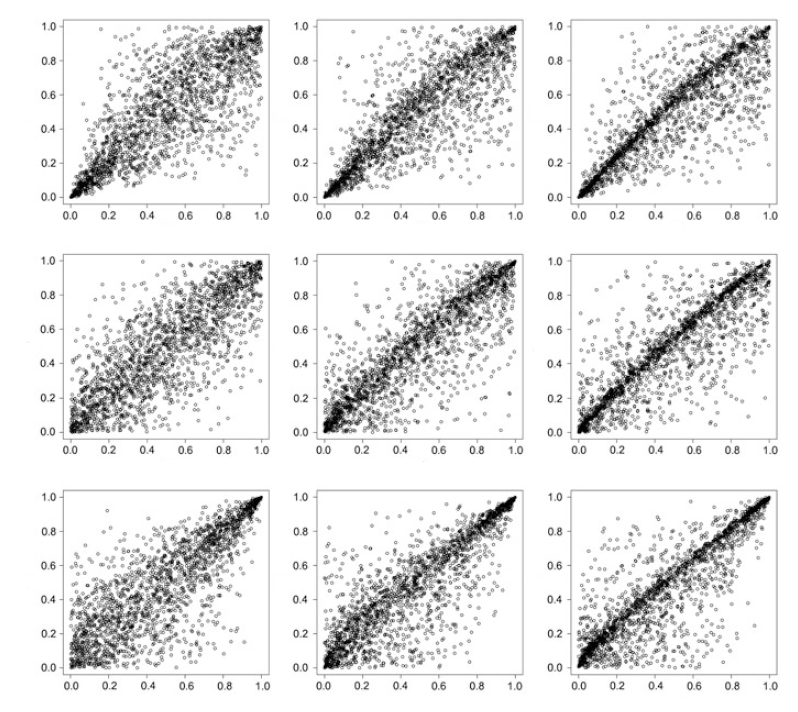
\includegraphics[width=0.7\linewidth]{./work/04-archimax/figures/Samples_Archimax_v02} 

}

\caption{Samples of size 2,000 drawn from different Archimax copulas with Gumbel's asymmetric Pickands dependece function, where Khoudraji's device with $\lambda = 0.5$ and $\kappa = 0.7$ is used to induce asymmetry. The parameter of the Gumbel's dependence function varies from left to right, i.e. it assumes three different arbitrary values (see \citet{genest2013}, p. 102 and p. 107 and references therein for details). For $\phi$, the Clayton (top row), Frank (middle row), and Joe (bottom row) Archimedean generators are used, where the corresponding parameter is chosen such that Kendall's tau of the Archimedean copula with generator $\phi$ equals 0.5. In every of the scatter plots presented above, the x-axis shows the values of the first component of the realizations drawn from the respective Archimax copula, while the y-axis shows the value of the respective second component. Adapted from \citet{genest2013}, p. 107.}\label{fig:archSmplsClaudia}
\end{figure}

\section{Conclusion}\label{concl}

Compound events are caused by at least two climate variables and the dependence between these climate variables can be asymmetric. This chapter laid the theoretical foundation for modelling compound events characterized by asymmetric dependence. Specifically, by reviewing the relevant literature, this chapter investigated how to recognize asymmetric dependence between two random variables and if and to what extent this asymmetric dependence can be modelled via Archimax copulas. For doing so, first, theoretical background about copulas in general was given, which allowed for making the concept of asymmetry in the dependence structure of random variables precise. Then, it was explained how this asymmetry can be measured based on the axiomatic approach developed by \citet{durante2010a}. Thus, the foundation for estimating the degree of asymmetry in the dependence structure of two random variables from real-world data as well as for measuring the theoretical degree of asymmetry in Archimax copulas was laid. In the next step, bounds for these asymmetry measures were presented, which allowed for normalization and thus supports interpretation of the values these measures assume. For illustration, an application of a selection of the asymmetry measures to hydrological data was presented. Finally, the concept of Archimax copulas was explained, which form a relatively broad class of copulas in the sense that they include the well-known Archimedean and extreme value copulas as special cases. Since Archimax copulas are only symmetric under a condition which was stated in section \ref{asymarchi}, they can be used for modelling asymmetric dependence between random variables. However, the degree of asymmetry in Archimax copulas is limited by an upper bound presented in section \ref{asymarchi}. The specific value this upper bound assumes depends on the generator \(\phi\) and the upper bound is reached if and only if the dependence function \(A\) takes one of two specific forms (see section \ref{asymarchi} for details). However, Archimax copulas are more flexible in modelling asymmetric dependence structures than one of their special cases, the extreme value copulas, which can also be asymmetric (see section \ref{asymarchi} as well as \citet{genest2013}, pp.~101-103 and \citet{durante2010b} for details).

Due to its scope, the focus of this chapter was on Archimax copulas. However, these copulas do not represent the only approach for modelling asymmetric dependence. In future work, one could compare different approaches for modelling this type of dependence structure, for which chapter 5.4, in \citet{genest2013} might be a good starting point. Moreover, as already explained in section \ref{intro}, this chapter focused on the asymmetry property of Archimax copulas. This however, is not the only property of these copulas. For example, one property, which might be interesting in the context of the climate crisis, is that Archimax copulas can be constructed with a predetermined extreme value attractor (see \citet{caperaa2000} for details). Also this might be worth further investigation, for which \citet{caperaa2000} as well as \citet{chatelain2020} could serve as starting points. In terms of asymmetry measures, this chapter focused on a certain class of asymmetry measures, which is in line with the axiomatic approach established by \citet{durante2010a} (see section \ref{backgrmeas}). Investigating alternative measures in more detail and comparing them to the ones explained above might be another interesting question one could address in the future.

\chapter{Teleconnections North Atlantic Oscillation}\label{nao}

\emph{Author: Pamela Sorelle Tueam}

\emph{Supervisor: Henri Funk}

\emph{Suggested degree: Bachelor}

\section{Abstract}\label{abstract-2}

The concept of teleconnections in climate science refers to climate anomalies or patterns that are related across large distances, often thousands of kilometers apart. Teleconnections represent atmospheric interactions that link weather and climate conditions in one region of the globe with those in another, often through the movement and behavior of large-scale atmospheric wave patterns (\citet{feldstein2017}). These connections are crucial for understanding regional climate variations, predicting weather patterns, and assessing climate change impacts. One prominent example of a teleconnection pattern in the Northern Hemisphere is the North Atlantic Oscillation (NAO). This oscillation plays a significant role in influencing the climate over the North Atlantic region. Its impacts are observed in various climate elements, including temperature, wind speed and direction, storm and precipitation, as well as ocean and sea ice dynamics. \(\\\)
This chapter explores various methods for defining and analyzing the North Atlantic Oscillation (NAO), following the framework established by \citet{hurrell2010}. These methods include one-point correlation map, Empirical Orthogonal Function (EOF) analysis, and cluster analysis. Additionally, we present the long-term trends of the NAO using the NAO Index. Through a detailed examination of these approaches, we aim to provide a better understanding of the spatial and temporal characteristics of the NAO. Such understanding is important for improving climate models, enhancing weather prediction accuracy, and developing robust climate change adaptation and mitigation strategies. Furthermore, by assessing the NAO's influence on temperature, wind patterns, storm activities, and oceanographic conditions, this chapter contributes to a deeper comprehension of how large-scale atmospheric phenomena shape our climate system.

\section{Introduction}\label{introduction-3}

The North Atlantic Oscillation (NAO), one of the most prominent and recurrent teleconnections over the Northern Hemisphere, is characterized by a redistribution of atmospheric mass at sea level between the Icelandic Low and the Azores High (\citet{hurrell2010}). It dictates climate variability from the eastern seaboard of the United States to Siberia and from the Arctic to the subtropical Atlantic, especially during boreal winter. Fluctuations from one phase of the NAO to another result in significant variations in the average wind speed and direction over the Atlantic, as well as in the transport of heat and moisture between the Atlantic and neighboring continents. This also affects the intensity and number of storms, their paths, and associated weather conditions (\citet{hurrell2003}). Especially during the months of December to March, the NAO is responsible for much variability of weather over the North Atlantic region. Thus, the NAO influences weather and climate conditions across the North Atlantic region and beyond, affecting winter temperatures and storm tracks. \(\\\)
In this chapter, our primary focus will be on exploring the spatial and temporal characteristics of the NAO. We will begin by discussing common methods used to define it, such as the one-point correlation map, which helps to identify the NAO by regions of positive and negative correlations. Additionally, we will employ the EOF analysis to discern the dominant patterns of variability associated with the NAO, and utilize the cluster analysis to identify distinct atmospheric patterns with similar pressure characteristics. Furthermore, we will analyze the NAO Index to observe its variations over long periods. Finally, we will investigate the impacts of the NAO on various climate factors including temperature, wind speed and direction, precipitation patterns, storm activities, oceanic conditions, and sea ice dynamics.

\section{The spatial and temporal structure of the NAO}\label{the-spatial-and-temporal-structure-of-the-nao}

Understanding NAO requires a comprehensive understanding of its spatial and temporal characteristics. To analyze these aspects, we will review established methods commonly employed for defining or identifying NAO patterns. These methods include the one-point correlation map, the EOF analysis for its spatial structure, as well as cluster analysis. For its temporal structure, we will focus on the NAO index. These methods are used in the paper of (\citet{hurrell2010}) and the data used in his paper go up to 2006. The idea is to reproduce these on new data up to 2024 and see if the NAO patterns remain similar.

\subsection{Data}\label{data-1}

Monthly geopotential height at 500 hPa (Z500) and mean sea level pressure (MSLP) data are used in this chapter. The monthly geopotential height at 500 hPa were obtained from the ERA5 reanalysis dataset for global climate and weather (\citet{geopotential2023}).
Mean sea level pressure data used here were also sourced from the ERA5 reanalysis (\citet{mean_sea_level2023}) dataset. For both monthly geopotential height and mean sea level pressure, only data from the Northern Hemisphere specifically within the coordinates 20°-70°N and 90°W-40°W, were extracted. Considering that the NAO is responsible for much variability of weather in boral winter over the Northern Hemisphere, the period from December to March (DJFM) was selected for this analysis. The time series used consist of 84 DJFM seasons from 1940-2024. The data used to examine the NAO Index were collected from the National Center for Atmospheric Research (NCAR). This dataset includes station-based NAO index data of 159 DJFM seasons spanning from 1864 to 2023 (\citet{nao_index_2003}). To examine the pattern of variability we need to compute the anomalies which are calculated by subtracting time means, computed for each calender month from the data for individual year-months. These anomalies form the basis for all methods described in this chapter.

\subsection{One-point correlation maps}\label{one-point-correlation-maps}

One way to define the NAO is through conceptually simple one-point correlation map, identifying the NAO by regions of maximum negative correlation over the North Atlantic. For these one-point correlation we will focus on the methods described by \citet{athanasiadis2009} and by \citet{wallace1981} in their respective papers. \(\\\)
One-point correlation correlates a variable at a specific location with the same variable at other locations. Given a field of data, we compute the correlation coefficient between the base point - referred to as the center of action - and each other points. The center of action is a specific location defined by latitude and longitude. The resulting correlation values generate a map that identifies the NAO by regions of positive and negative correlation. In this analysis, we use monthly geopotential heights data at 500 hPa for winter season December-March from 1940 to 2024. Anomalies are calculated by subtracting geopotential height time means, computed for each calendar month from the data for individual geopotential height year-months (\citet{wallace1981}, 790). \(\\\)
The correlation coefficient for a given center of action is calculated using the Pearson's linear correlation coefficient at every point as follows:

\(r_{i} = \frac{Cov(X_{i}, Y_{i})}{\sqrt{Var(X)Var(Y)}}\)

where X and Y are time series of contemporaneous observations, \([(x_{i}, y_{i}); i = 1, 2, . . . N]\), where we fix one of the data points, say, X, at the center of action and compute the correlation over all Y. Covariance and variance are denoted as Cov and Var, respectively (\citet{athanasiadis2009}, 3721). \(\\\)
Figure \ref{fig:CorrelationPamela} illustrates the corresponding one-point correlation map for the NAO pattern. The reference point that has been chosen is located in Iceland at 65°N and 18°W. The correlations are calculated for all points belonging to the Northern Hemisphere (20-70°N, 90°W-40°E).
As we can see on the figure the map is characterized by more or less elliptical regions where correlation coefficients can be positive or negative, surrounding each base grid point. The size of these regions provides an indication of the horizontal scale of the anomalies, particularly near the base grid points (\citet{wallace1981}, 790).
The identifying dipole patterns located at the Icelandic Low and Azores High, reflect the NAO signature based on the chosen reference point. The color gradients on the figure indicate the strength of the correlation, with blue representing negative correlations and yellow to red representing positive correlations. \(\\\)
As implications, regions with strong positive correlations experience atmospheric conditions similar to Iceland (the center of action). These areas may share similar temperature anomalies. For instance, if the region of the center of action experiences warmer-than-average temperatures during high NAO phase, positive correlated regions might also experience similar warmth temperatures. We will also have similar precipitation patterns (if it is drier than the nearby regions may also be similar dry). Conversely, the region with negative correlations such as the anticorrelation center at Azores, will exhibit opposite conditions, including temperature contrasts (warmer vs.~cooler) and differing precipitation patterns (wetter vs.~drier).

\begin{figure}

{\centering 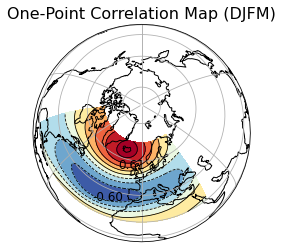
\includegraphics[width=0.5\linewidth]{work/05_nao/figures/OnePointCorrelation} 

}

\caption{One-point correlation map of 500 hPa geopotential height for boreal winter (December-March) over 1940-2024. The reference point is 65°N, 18°W. Negative correlation coefficients are in blue and the lines are dashed.}\label{fig:CorrelationPamela}
\end{figure}

\subsection{EOF Analysis}\label{eof-analysis}

The second method is the Empiriacal Orthogonal Function (EOF) analysis, also known as Principal Component Analysis (PCA). EOF analysis is commonly used to identify and analyze dominant patterns of variability in spatial and temporal datasets. The EOFs of a dataset are simply the eigenvectors of the covariance matrix of the dataset, which provide maximal data compression (\citet{wilks2011}). The method reduces a dataset with many variables to a smaller set of new variables, which are linear combinations of the original ones, chosen to capture the maximum possible variability of the original data (\citet{wilks2011}). Given multiple observations of a (K × 1) data vector \(\textbf{x}\), PCA finds (M x 1) vector \(\textbf{u}\), which are linear combinations of the elements of \(\textbf{x}\) and capture most of the information from the original data (\citet{wilks2011}). The steps by performing the EOF are as follows:

\begin{itemize}
\tightlist
\item
  Collection of the dataset: We used the mean sea level pressure (MSLP) data for boreal winter DJFM over 84 years from 1940 to 2024.
\item
  Calculation of the anomalies: Anomalies are calculated by subtracting the MSLP time means, computed for each calendar month from the data for individual MLSP year-months.
\item
  Formation of the Covariance Matrix as we want to analyze the variance and patterns in the data.
\item
  Performance of the eigenvalue decomposition: The covariance matrix is decomposed using eigenvalue decomposition to obtain the eigenvalues and eigenvectors. The eigenvectors represent the spatial patterns, and the eigenvalues indicate the amount of variance explained by each EOF.
\item
  The first principal component, \(u_{1}\) is obtained as the projection of the anomalies vector onto the first eigenvector \(\textbf{e}_{1}\) \(\textbf{u}_{1} = \textbf{e}_{1}^{T} = \sum_{k= 1}^{K} e_{k, 1}x_{k}^{'}\). This first EOF/PC explains the most variance, followed by the second, and so on (\citet{wilks2011}).
\end{itemize}

Computing the EOFs allows for comparison with the results of the one-point correlation analysis. While correlation analysis focuses on the variability relative to the primary center of action of specific teleconnections, EOF analysis is not centered on specific points. The loading at any two points are not solely determined by the temporal correlation between the time series at those points (\citet{athanasiadis2009}, S 3724). Furthermore, EOF analysis is not explicitly designed to highlight regional patterns of strong correlation. Instead, EOF analysis sequentially identifies the leading patterns that explain the most variance within the analyzed dataset (\citet{athanasiadis2009} S 3724). Therefore, values of the same sign at two different spatial points in an EOF do not necessarily imply a significant correlation between those two points.

Figure \ref{fig:EofPamela} illustrates the leading eigenvectors of the cross-covariance matrix calculated from seasonal (4-month average) MSLP anomalies in the North Atlantic sector (20°-70°N; 90°W-40°E). Since the eigenvectors are, by definition, structured to explain maximum variance, it is expected that the center of actions of the leading EOFs will coincide with the regions of strongest variability. Although EOF patterns are not exactly identical to the one-point correlation map, there is a noticeable similarity between the two. Both correlation map and EOF analysis consistently illustrate the distinct behavior of variability across different time scales. During the winter season (December-March), the NAO accounts for more than one-third (35.8\%) of the total variance in SLP over the North Atlantic and appears with a slight northwest-to-southeast orientation.

\begin{figure}

{\centering 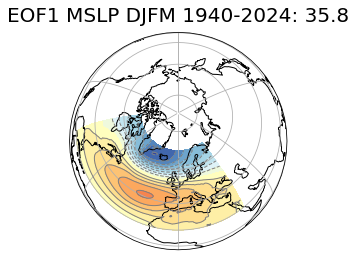
\includegraphics[width=0.6\linewidth]{work/05_nao/figures/EOF1} 

}

\caption{Leading empirical orthogonal function (EOF 1) of the seasonal mean sea level pressure anomalies in the North Atlantic sector (20°–70°N, 90°W–40°E), and the percentage of the total variance it explains. The data cover the period of 1940–2024.}\label{fig:EofPamela}
\end{figure}

\subsection{Cluster Analysis}\label{cluster-analysis}

Another method to examine the dynamical signature of interannual variability in the North Atlantic is the cluster analysis. This non-linear approach groups similar data points into clusters based on their similarities, and is used here to identify distinct atmospheric patterns with similar pressure characteristics. It is applied to 84 years of monthly MSLP data from December to March using procedures based on a clustering algorithm. The algorithm groups in this case the monthly MSLP data into a small number of representative states (or regimes) according to an objective criterion of similarity.
Given a prescribed number of clusters \(k\), the goal of the algorithm is to find a partition \(P\) of the data points into \(k\) clusters \(C_{1}, C_{2}, …, C_{k}\) that minimizes the sum of the variances within the clusters, expressed as (\citet{michelangeli1995}): \[W(P) = \sum_{j= 1}^k \sum_{x \in C_{j}} d^2(X, Y_{j})\] where \(Y_{j}\) is the centroid cluster \(C_{j}\) and \(d(X, Y)\) represents the Euclidean distance between two points X and Y as a measure of similarity. The global minimum of the function \(W(P)\) therefore corresponds to a partition that achieves the best separation of data points. The dynamic cluster algorithm defines iterative partitions \(P^{(n)}\) for which \(W(P^{(n)})\) decreases with n and eventually converges to a local minimum which generally differs from the global one. This algorithm thus provides the optimal \(k\) number of clusters to be retained (\citet{michelangeli1995}, S 1241).
The steps by performing the cluster Analysis are:

\begin{itemize}
\tightlist
\item
  Data collection and anomalies calculation.
\item
  Selection of a clustering algorithm: In this case the k-means clustering is used.
\item
  Determination of the optimal number of clusters.
\item
  Application of the algorithm: Assign each monthly SLP data to a cluster with each cluster representing a distinct atmospheric regime or pattern.
\end{itemize}

The clustering algorithm applied over the Atlantic domain (20°--70°N; 90°W--40°E) identifies four winter climate regimes Figure \ref{fig:RegimesPamela}. The clustering partition yields the optimal \(k = 4\) number of significant winter climate regimes subsequently represented by the cluster centroid. Two of these clusters correspond to the negative and positive phases of the NAO and are characterized by a zonally elongated meridional pressure dipole between the Icelandic Low and the Azores High. The third regime exhibits a zonal pressure dipole between Greenland and Scandinavia (the ``Blocking'' regime) with a clear southeastward extension of low-pressure anomalies toward the Iberian Peninsula. The fourth regime displays a strong anticyclonic ridge (RDG) over western Europe (the ``Atlantic Ridge'' regime) (\citet{hurrell2010}).

\begin{figure}

{\centering 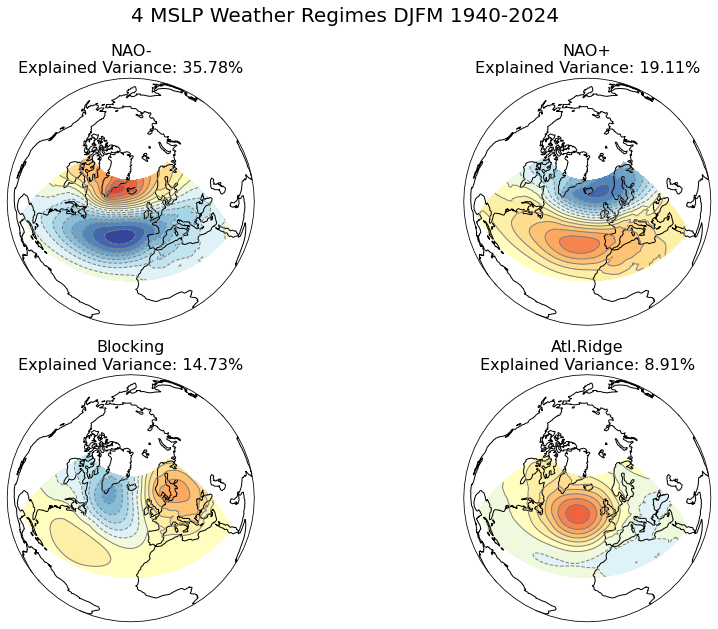
\includegraphics[width=0.7\linewidth]{work/05_nao/figures/ClusterAnalysis} 

}

\caption{Boreal winter (December–March) climate regimes in sea level pressure (hPa) over the North Atlantic domain (20°–70°N, 90°W–40°E) using monthly data over the period from 1940 to 2024. The percentage on each panel expresses the explained variance of each cluster.}\label{fig:RegimesPamela}
\end{figure}

\subsection{NAO positive and negative Index}\label{nao-positive-and-negative-index}

The most modern NAO indices are derived either from the simple difference in surface pressure anomalies between selected northern and southern locations, or from the PC time series of the leading Empirical Orthogonal Function (EOF) of the sea level pressure (SLP) field (\citet{hurrell2010}). Although the NAO is observable throughout the year, it is most pronounced during winter, accounting for over one-third of the total variance in the SLP field over the North Atlantic (\citet{hurrell1997}, 305). (\citet{hurrell1997}) defined a simple index of the NAO as the difference between the normalized mean winter (December--March) SLP anomalies at Lisbon, Portugal and Stykkisholmur, Iceland.

Figure \ref{fig:IndexPamela} illustrates the positive and negative index of the NAO from 1864 to 2023. The average winter sea level pressure data at each station were normalized by division of each seasonal pressure by the long-term mean (1864--2023) standard deviation. Positive values of the index are in red and negative values in blue. The NAO index, as depicted in Figure \ref{fig:IndexPamela}, exhibits a well-defined oscillation. However, several periods exist where the NAO index remained in one phase over multiple winters, such as from 1903 to 1914 (positive phase), from 1915 to 1919 (negative phase), from 1958 to 1971 (negavite phase, excluding 1961 and 1967), and from 2014 to 2020 (posivite phase). On this figure of the NAO index \ref{fig:IndexPamela} we can notice that there is little evidence for the NAO to vary on any preferred time scale. Significant changes can occur from one winter to the next, as well as from one decade to another.\(\\\)

\begin{figure}

{\centering 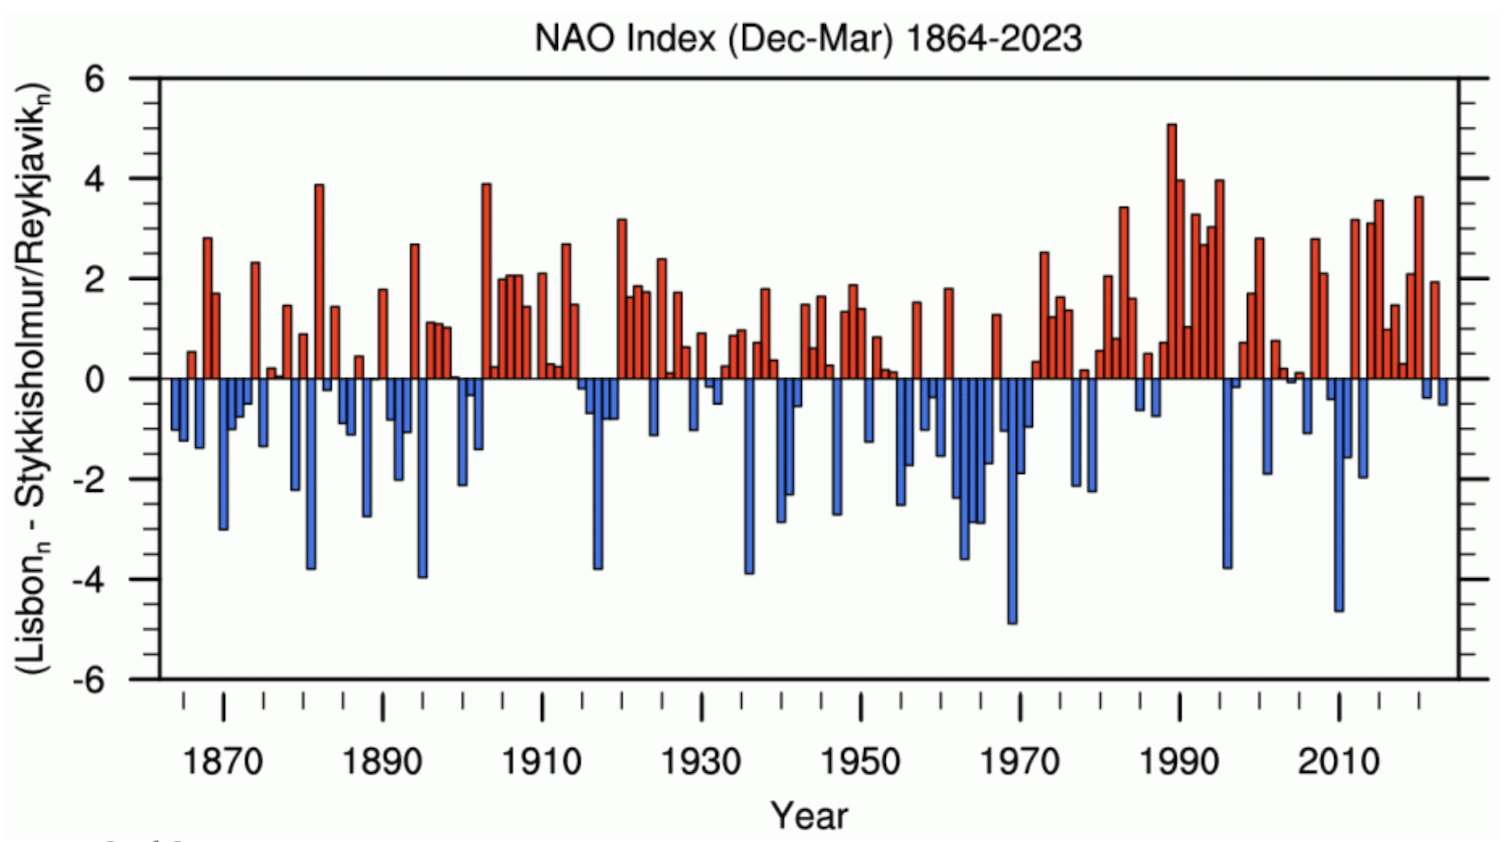
\includegraphics[width=0.8\linewidth]{work/05_nao/figures/NAOIndex} 

}

\caption{Normalized indices of the mean winter (December–March) NAO constructed from sea level pressure data. The index is based on the difference of normalized sea level pressure between Lisbon, Portugal and Stykkisholmur/Reykjavik, Iceland. The average winter sea level pressure data at each station were normalized by division of each seasonal pressure by the long-term mean (1864–2023) standard deviation. The indicated year corresponds to the January of the winter season (e.g, 1990 is the winter of 1989/1990)}\label{fig:IndexPamela}
\end{figure}

The NAO is in a positive phase when both Icelandic low-pressure center and the high-pressure center at the Azores are stronger than the average (figure \ref{fig:phasePamela}). During the positive NAO phase, the increased difference in pressure between these two regions results in a stronger Atlantic jet stream and a northward shift of the storm track. Consequentlly, northern Europe experiences increased storminess, higher precipitation, and warmer-than-average temperatures due to the air masses that arrive from lower latitudes. At the same time, southern Europe experiences decreased storminess and below-average precipitation. In eastern North America, the positive phase of the NAO generally brings higher air pressure, a condition associated with fewer cold-air outbreaks and decreased stormisses (\citet{hurrell2010}).

Conversely, the NAO is in a negative phase when both the Icelandic low and Azores high are weaker than average. During the negative NAO phase, the Atlantic jet stream and storm track have a more west-to-east orientation. This results in decreased storminess, below-average precipitation, and lower-than-average temperatures in to northern Europe. Conversely, southern Europe experiences increased storminess, above-average precipitation, and warmer-than-average temperatures. In eastern North America, the negative phase of NAO generally brings lower air pressure, a condition associated with stronger cold-air outbreaks and increased storminess (\citet{hurrell2010}).

\begin{figure}

{\centering 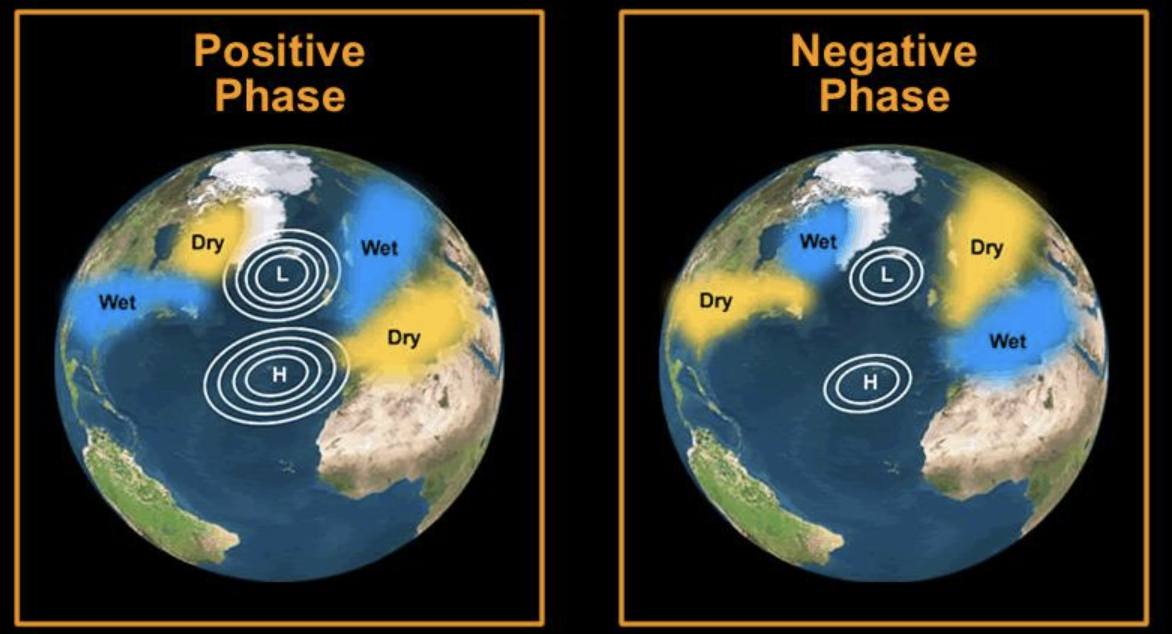
\includegraphics[width=0.7\linewidth]{work/05_nao/figures/NAOPhase} 

}

\caption{Positive and negative phase of the North Atlantic Oscillation. Image from @NAO\_phase2013}\label{fig:phasePamela}
\end{figure}

\section{The Implications of the North Atlantic Oscillation}\label{the-implications-of-the-north-atlantic-oscillation}

The NAO plays a critical role in shaping climate patterns across the North Atlantic and surrounding areas. Changes in its spatial and temporal structures can lead to significant variations in temperature, precipitation, and weather extremes, influencing ecosystems, human activities, and natural resources.

\subsection{Temperature, wind speed and direction}\label{temperature-wind-speed-and-direction}

During the positive phase of the North Atlantic Oscillation (NAO), the atmospheric pressure difference between the Icelandic low and the Azores high intensifies. This results in a stronger-than-usual westerly flow across the North Atlantic during the winter months. Consequently, relatively warm, and moist maritime air is transported over much of Europe and extends across Asia (\citet{hurrell2003}). This influx of warm air can lead to milder winter conditions across the continent, often resulting in higher temperatures (\citet{hurrell2003}). Meanwhile, while stronger northerly winds over Greenland and northeastern Canada transport cold air southward leading to a decrease in land temperatures in the northwest Atlantic (\citet{hurrell2003}). The cold air intrusions can lead to harsher winter conditions in parts of eastern Canada and the northeastern United States. \(\\\)
Additionally, the stronger clockwise circulation around the subtropical Atlantic high-pressure center during this phase of the NAO significantly impacts other regions. In North Africa and the Middle East, this results in cooler-than-average temperatures due to the altered wind patterns. In contrast, parts of North America experience warmer conditions as the strengthened high-pressure system influences the weather patterns across the continent (\citet{hurrell2003}).

\subsection{Storm and precipitation}\label{storm-and-precipitation}

NAO signals can also be found in winter precipitation and storm over the North Atlantic.During the positive phase of the NAO, storm activities in the Atlantic shift northeastward. This means there are more intense and frequent storm activities from southern Greenland across Iceland into northern Europe, and slightly less storm activities from the Azores across the Iberian Peninsula and the Mediterranean (\citet{hurrell2010}). Furthermore, the positive phase is typified by more intense and frequent storms in the vicinity of Iceland and the Norwegian Sea. During the NAO-, a weak subtropical high and a weak Icelandic Low dominate, resulting in a reduced pressure gradient and fewer, weaker winter storms with a more west-east trajectory, while moist air is brought into the Mediterranean and cold air into northern Europe (\citet{rousi2020}).
\(\\\)
Changes in the mean flow and storminess associated with oscillations in the NAO index lead to significant changes in the transport and convergence of atmospheric moisture, impacting the distribution of evaporation and precipitation (\citet{hurrell2010}). These results in drier conditions of this magnitude are observed over central and southern Europe, the Mediterranean, and parts of the Middle East, while more precipitation than normal occurs from Iceland through Scandinavia (\citet{hurrell2010}).

\subsection{Ocean and Sea Ice}\label{ocean-and-sea-ice}

Another implication of the NAO mentioned by \citet{hurrell2010} is its impact on ocean and sea ice. SST and NAO strength fluctuate together, with the main pattern of SST variability in boreal winter forming a tri-polar structure: a cold anomaly in the subpolar North Atlantic, a warm anomaly in mid-latitudes, and a cold anomaly in subtropical regions (\citet{hurrell2010}). These SST anomalies are driven by changes in surface wind and air-sea heat exchanges related to NAO variations. Persistent SST anomalies over longer periods also relate to consistent anomalous SLP patterns, including the NAO, reflecting the ocean's response to long term atmospheric variability.
The reduction of the Arctic Sea ice is one of the most prominent indicators of climate change. less compact ice in high NAO winters plays an important role in the reduction of summer sea ice extent in high NAO years. In winter, the stronger wind in high NAO years drives more ice away from the Eurasian coastal region, suppressing sea ice buildup there (\citet{hurrell2003}).

\section{Conclusion}\label{conclusion-2}

In this chapter we have presented the NAO as the dominant mode of regional climate variability over the Northern Hemisphere, focusing particularly on common methods used to identify its spatial and temporal structure. These methods, although they are different, each have their strengths and limitations.
One point correlation map is easy to implement and interpret providing clear insight into how the chosen center of action is related to the variability at other locations. However, the result heavily depends on the choice of the center of action. Selecting a different center may not well capture the full spatial pattern of the NAO. EOF analysis captures the dominant patterns of variability in a dataset and provides a quantitative measure of how much variance a pattern explains. But it assumes linear relationships and might not capture non-linear features of the NAO. Cluster Analysis is effective at identifying distinct patterns and regimes including non-linear and non-stationary features, but it is computationally intensive and requires careful selection of clustering parameters. Additionally, interpreting the results can be challenging if the patters are not well separated.

As we have seen, the NAO is a significant climatic driver in the North Atlantic region, influencing temperature, wind speed and direction, precipitation, storm tracks, ocean and sea ice, particularly over Europe and North America. Its variability poses challenges and opportunities for understanding and predicting weather and climate impacts in affected regions. Understanding the implications of the NAO for climate change is essential for developing adaptive strategies to deal with the resulting implications on weather patterns and sea ice.

By improving climate models, and implementing robust adaptation plans, we can better address the challenges posed by NAO-induced climate variability. Predicting the future behavior of the NAO in a changing climate is challenging due to the complexity of the interactions between the atmosphere, oceans, and sea ice. Enhanced climate models that incorporate these interactions are crucial for reducing uncertainties and improving forecasts. Despite the strong influence of the NAO, many open issues remain about which climate processes govern NAO variability, how the phenomenon has varied in the past or will vary in the future, and to what extent it is predictable. External factors, such as the rise in greenhouse gas emissions, have a significant impact on the recent patterns of the NAO (\citet{gillett2003}). Research indicates that higher greenhouse gas concentrations are associated with alterations in atmospheric circulation, which may result in more frequent occurrences of positive NAO phases (\citet{gillett2003}). Understanding these shifts is essential for developing strategies to mitigate and adapt to the climate change effects influenced by the NAO (\citet{gillett2003}).

\chapter{Low Flow Events}\label{lfe}

\emph{Author: Gamze Gizem Kasman}

\emph{Supervisor: Henri Funk}

\emph{Degree: Master}

\section{Abstract}\label{abstract-3}

This chapter introduces some of the most used advanced statistical methods for predicting and analyzing low-flow events, characterized by reduced streamflow and water availability. Initially, key univariate concepts such as nonstationary models with time-varying parameters and meteorological covariates are presented, along with the concept of return periods to capture the dynamic nature of these events accurately. Following this, bivariate concepts, including the use of copulas to model dependencies between hydrological variables and the integration of reservoir indices to account for human impacts on flow regimes, are discussed. The concept of return periods is also introduced in a bivariate context. After these theoretical introductions, the chapter demonstrates practical applications, including the Statistical Downscaling Model (SDSM), which connects large-scale climate projections with localized hydrological impacts. These methodologies enhance the prediction and management of low-flow events, offering more robust strategies for water resource management in a changing climate.

\section{Introduction}\label{introduction-4}

Low-flow events or periods are hydrological conditions marked by significantly reduced streamflow and water availability in rivers and streams. These events often result from prolonged dry weather conditions, reduced precipitation, high evaporation rates, or significant water withdrawals (\citet{Smakhtin2001}). Their extremeness distinguishes them from normal variations in water flow, as they can profoundly and lastingly impact water availability and quality.

To effectively manage and mitigate the consequences of these extreme low-flow periods, it is essential to predict their occurrence and severity. This is where the concept of return periods becomes crucial. The return period, also known as the recurrence interval, is a statistical measure that estimates the frequency at which a particular hydrological event, such as a low-flow period, is expected to occur (\citet{Stedinger1993}). It provides a probabilistic assessment of how often extreme low-flow events of a certain magnitude are likely to happen over a given time frame. The concept of return periods is mostly used in the context of univariate analysis, where it pertains to a single hydrological variable, such as streamflow. However, return periods are also utilized in bivariate analysis in the context of low-flow events. Bivariate return periods consider the joint occurrence of two hydrological variables, such as streamflow and precipitation, or the dependence between two low-flow series, providing a more comprehensive assessment of extreme events. The bivariate approach is particularly useful when the interaction between variables significantly influences the event's occurrence and impact (\citet{Graler2013}; \citet{Salvadori2007}).

Closely associated with the return period is the concept of risk. In the context of hydrology, risk refers to the probability that a specific event, such as a low-flow period, will occur within a given timeframe. Understanding the risk associated with different return periods allows water resource managers to better prepare for and mitigate the impacts of these extreme low-flow events, ensuring more resilient and adaptable water management practices.

Climate change adds a significant layer of complexity to the management and prediction of low-flow events. Changes in climate patterns, such as alterations in precipitation regimes and increased temperatures, can exacerbate the frequency and severity of low-flow periods. For instance, climate change may lead to longer dry seasons, reduced snowpack, and increased evapotranspiration, all of which contribute to more severe low-flow conditions (\citet{Katz1992}). Furthermore, shifts in weather extremes mean that historical data may no longer be a reliable predictor of future conditions, complicating the estimation of return periods and associated risks. Therefore, understanding how flood and low-flow events are evolving and how likely they are to unfold beyond their historical distributions under the influence of multiple drivers, such as climate variability, human activities like reservoir operations etc., is one of the major challenges facing the hydrology field (\citet{Lopez2013}; \citet{Kam2016}; \citet{Gai2019}; \citet{Jiang2021}; \citet{Slater2021a}). In particular, predicting the likelihood of low-flow events occurring beyond their historical distributions due to factors like climate variability and human activities remains a key challenge in hydrology (\citet{Lopez2013}; \citet{Kam2016}; \citet{Gai2019}; \citet{Jiang2021}; \citet{Slater2021a}; \citet{Wang2022}).

This necessitates the use of advanced statistical models that can incorporate climate projections, climate indices such as oscillation data, and reservoir indices to better predict low-flow events in a changing climate (\citet{Coles2001}). Understanding how climate change impacts low-flow events and their return periods is crucial for adapting water management practices to future conditions.

This chapter aims to provide a focused study on low-flow events and their return periods through a statistical lens. We will introduce and discuss the most widely used models in hydrological frequency analysis that take climate change and human activities into account. These modern methods incorporate a variety of data sources, providing a more accurate prediction of low-flow events under changing climate conditions. For comparison purposes, we will also present traditional approaches that do not account for climate change, which assume that the statistical properties of low-flow events remain constant over time. By exploring both modern and traditional methods, we will highlight their respective advantages and limitations, and demonstrate their applications in the context of hydrological frequency analysis of low-flow events and return periods.

\section{Data Analysis}\label{data-analysis}

In the context of hydrological frequency analysis, understanding the most commonly used datasets that underpin our insights into low-flow events and return periods is essential. These datasets vary in their sources, methodologies, and applications, reflecting advancements in the field and the growing acknowledgment of climate change.

\subsection{Observed Hydrological Data}\label{observed-hydrological-data}

One of the foundational datasets in hydrological analysis is observed hydrological data, which encompasses both temporal and spatial dimensions. This data, typically gathered from gauging stations along rivers and streams, captures key measurements such as river discharge, water levels, and flow rates. The temporal aspect is reflected in the continuous time-series records, while the spatial aspect is evident in the geographical distribution of gauging stations across a watershed. The value of this data lies in its direct representation of the hydrological processes within a given watershed, providing a reliable basis for understanding past and present flow conditions.

Long-term records from these stations are crucial for identifying trends, variability, and the statistical characteristics of hydrological events, including low-flow and high-flow occurrences. This type of data can be directly utilized in statistical analyses for hydrological frequency analysis, enabling researchers to assess event probabilities and predict future hydrological behaviors (\citet{Helsel2002}).

\subsection{Observed Meteorological Data}\label{observed-meteorological-data}

In the context of models where climate change is acknowledged, observed meteorological data plays a significant role. This dataset encompasses measurements of various atmospheric parameters, including precipitation, temperature, and humidity, collected from meteorological stations. The linkage between meteorological conditions and hydrological responses is vital, as weather patterns significantly influence water availability and flow dynamics. By analyzing this data, researchers can better understand the drivers of hydrological extremes and their temporal patterns, thus enhancing the prediction and management of low-flow events in the context of a changing climate (\citet{Huntington2006}). Initially, this data is point data as it is collected from individual meteorological stations. It is then spatially averaged to form areal data representing the broader catchment areas.

\subsection{Reanalysis Data}\label{reanalysis-data}

Reanalysis data adds another critical dimension to modern hydrological studies. These datasets synthesize historical weather observations with modern forecasting models to produce comprehensive and consistent records of atmospheric conditions over extended periods. An example of this is the NOAA National Centers for Environmental Prediction (NCEP) reanalysis data. This data offers high temporal and spatial resolution, filling gaps where direct observations may be sparse or unavailable. Reanalysis data uses a variety of atmospheric predictors such as sea level pressure, air temperature at various altitudes, geopotential heights, and humidity, integrating them with observed data to create a continuous and coherent dataset (\citet{Kalnay1996}). This linkage to observed meteorological data ensures that reanalysis products accurately reflect past atmospheric conditions, making them a critical tool for studying long-term trends and variability in low-flow events under changing climatic conditions. This data is considered gridded spatial data due to its continuous spatial coverage over a global grid.

\subsection{Global Circulation Model Outputs}\label{global-circulation-model-outputs}

Another dataset for hydrological frequency analysis comes from climate modeling efforts. General Circulation Models (GCMs) simulate the Earth's climate system, incorporating the interactions between the atmosphere, oceans, land surface, and ice. These models are integral to projecting future climate scenarios and assessing potential impacts on hydrological systems. The Coupled Model Intercomparison Project (CMIP), organized by the World Climate Research Programme (WCRP), is a key initiative that brings together various GCM outputs to facilitate a comparative analysis of these projections. The IPCC uses results from these GCMs to provide comprehensive assessments of future climate change in its reports. For hydrological frequency analysis, GCM outputs are crucial for assessing future scenarios of low-flow events under different greenhouse gas emission pathways. However, the coarseness of GCM outputs often requires them to be downscaled to a finer resolution to be useful for regional or local studies. GCM outputs are also gridded spatial data, providing large-scale projections over a global grid. Downscaling techniques, which can be statistical or dynamical, help bridge the gap between the broad, global scale of GCMs and the finer scales needed for practical hydrological applications. In this regard, NCEP reanalysis data is frequently used as a reference to improve the downscaling of GCM outputs, ensuring that they more accurately reflect observed climatic conditions at finer scales (\citet{Gao2012}).

\subsection{Reservoir Indices}\label{reservoir-indices}

Reservoir indices are critical datasets in hydrological studies, especially for understanding and managing low-flow events. These indices provide information on reservoir levels, inflows, outflows, storage capacities, and water releases. Reservoir operations significantly influence streamflow regimes, particularly during periods of low flow, by regulating the amount of water released downstream. The management of reservoir water levels can mitigate the impacts of droughts and ensure a stable water supply for various uses, including agriculture, drinking water, and hydroelectric power generation.

López and Francés (2013) proposed the reservoir index (RI) as an indicator of the impact of reservoirs on flow regimes. It is defined as follows:

\[ RI = \sum_{i=1}^{N}\left(\frac{A_{i}}{A_{T}}\right) \cdot \left(\frac{V_{i}}{C_{T}}\right) \tag{1}\]

where \(N\) is the number of reservoirs upstream of the gauge station, \(A_{i}\) is the catchment area of each reservoir, \(A_{T}\) is the catchment area of the gauge station, \(V_{i}\) is the total capacity of each reservoir, and \(C_{T}\) is the mean annual streamflow of the gauge station.

This definition may be modified in specific studies to better suit their research needs. The table below provides detailed information about the datasets used in these studies, including any modifications to the reservoir index.

\textbf{Data Used in Key Studies}

Throughout this chapter, information and results from the following studies will be referenced. The table below provides detailed information about the datasets used in these studies.

\textbf{Table: Detailed Information of Data Used in Studies}

\begin{longtable}[]{@{}
  >{\raggedright\arraybackslash}p{(\columnwidth - 8\tabcolsep) * \real{0.1221}}
  >{\raggedright\arraybackslash}p{(\columnwidth - 8\tabcolsep) * \real{0.1455}}
  >{\raggedright\arraybackslash}p{(\columnwidth - 8\tabcolsep) * \real{0.2723}}
  >{\raggedright\arraybackslash}p{(\columnwidth - 8\tabcolsep) * \real{0.0563}}
  >{\raggedright\arraybackslash}p{(\columnwidth - 8\tabcolsep) * \real{0.3897}}@{}}
\toprule\noalign{}
\begin{minipage}[b]{\linewidth}\raggedright
Study
\end{minipage} & \begin{minipage}[b]{\linewidth}\raggedright
Data Type
\end{minipage} & \begin{minipage}[b]{\linewidth}\raggedright
Details
\end{minipage} & \begin{minipage}[b]{\linewidth}\raggedright
Period
\end{minipage} & \begin{minipage}[b]{\linewidth}\raggedright
Source
\end{minipage} \\
\midrule\noalign{}
\endhead
\bottomrule\noalign{}
\endlastfoot
\textbf{Du et al.~(2015)} & Observed Hydrological Data & Mean daily streamflow data & 1954-2009 & Huaxian and Xianyang gauging stations \\
& Observed Meteorological Data & Daily average temperature and daily total precipitation & 1954-2009 & 22 meteorological stations in the Wei River Basin \\
& Reanalysis Data & NCEP reanalysis data & 1954-2009 & NOAA (National Oceanic and Atmospheric Administration) \\
& GCM Outputs & Downscaled GCM outputs & 2010-2099 & CMIP5 (Coupled Model Intercomparison Project Phase 5) under the RCP 8.5 scenario \\
\textbf{Wang et al.~(2022)} & Observed Hydrological Data & Mean daily streamflow data & 1955-2016 & Multiple gauging stations in the Yellow River Basin \\
& Observed Meteorological Data & Daily temperature and precipitation data & 1955-2016 & Meteorological stations in the Yellow River Basin \\
& Reservoir Data & Reservoir inflow, outflow, and storage capacity data & 1955-2016 & Reservoirs in the Yellow River Basin \\
\textbf{Jiang et al.~(2015)} & Observed Hydrological Data & Mean daily streamflow data & 1961-2010 & Ankang (Qa) and Huangzhuang (Qh) gauges \\
& Observed Meteorological Data & Daily temperature and precipitation data & 1961-2010 & Meteorological stations in the Weihe River Basin \\
& Reservoir Data & Reservoir inflow, outflow, and storage capacity data & 1961-2010 & Reservoirs in the Weihe River Basin \\
\end{longtable}

\section{Stationarity vs.~Nonstationarity in Low-flow Analysis}\label{stationarity-vs.-nonstationarity-in-low-flow-analysis}

In hydrological frequency analysis, understanding the concept of stationarity is crucial for predicting and managing low-flow events. Traditionally, hydrological analyses have assumed stationarity, meaning that the statistical properties of hydrological processes are constant over time. Under this assumption, the historical data on low-flow events can be used to predict future occurrences with the expectation that the governing processes and factors remain unchanged. This approach simplifies the analysis and provides a straightforward basis for calculating return periods and risks (\citet{Gilroy2012}; \citet{Katz2013}).

Stationary analysis operates under the premise that factors such as climate and land use, which influence hydrological events, do not change significantly over time. This allows for the use of historical data to estimate future low-flow events with a reasonable degree of confidence. The traditional frequency analysis methods, such as fitting probability distributions to historical low-flow data, rely on this assumption. These methods are useful for long-term planning and water resource management as they provide stable and predictable estimates of low-flow probabilities and return periods (\citet{Chow1988}). However, the assumption of stationarity is increasingly being questioned due to evident and ongoing changes in climate and land use patterns. Studies have shown that these changes can significantly alter hydrological processes, rendering stationary models less reliable(\citet{Milly2008}).

Nonstationary analysis acknowledges that the statistical properties of hydrological processes can change over time due to factors like climate change, urbanization, and land-use changes. In a nonstationary framework, the parameters of probability distributions used to model hydrological events are allowed to vary over time or with respect to external covariates, such as meteorological variables. This approach provides a more realistic representation of the evolving nature of hydrological processes under the influence of changing climatic and environmental conditions (\citet{Katz2002}; \citet{Milly2008}).

The most common method for addressing nonstationarity in hydrological time series is the time-varying moment method. This technique assumes that while the type of distribution function for the hydrological variable remains constant, its statistical parameters can vary over time (\citet{Strupczewski2001}; \citet{Coles2001}; \citet{Katz2002}; \citet{Villarini2009}; \citet{Gilroy2012}). The time-varying moment method is typically used in a univariate context, where it focuses on a single hydrological variable, adjusting its statistical parameters to reflect temporal changes. Furthermore, the time-varying moment method can be extended to perform covariate analysis by replacing time with physical factors known to influence the hydrological variable of interest, such as temperature and precipitation. This provides a dynamic model that can adapt to projected changes in climate. This approach is critical for modern water resource management as it helps anticipate the impacts of climate variability and change, thus supporting more resilient and adaptable planning and infrastructure development (\citet{Du2015}; \citet{Jiang2015}).

In addition to the time-varying moment method, copula-based models have become increasingly important in nonstationary hydrological analysis. Copulas allow for the modeling of complex interdependencies between hydroclimatic variables, such as streamflow, precipitation, and temperature, as well as the dependence structure between low-flow events. Copula models are particularly useful in a bivariate context, as they can capture the evolving dependencies between two or more variables over time or under changing climatic conditions. This capability is crucial for understanding and predicting compound extreme events, which occur due to the concurrence or succession of multiple hydroclimatic extremes. By using copula-based probability distributions, researchers can more accurately assess the risk and impact of such compound events, providing a more comprehensive approach to hydrological frequency analysis (\citet{Tootoonchi2022}).

Comparing stationary and nonstationary analyses highlights the limitations of traditional methods in the face of a changing climate. Stationary models, while simpler and easier to apply, may lead to underestimation or overestimation of future low-flow events if the underlying conditions change significantly. Nonstationary models, though more complex, offer a nuanced understanding by integrating evolving environmental variables into the analysis, thus providing more accurate and reliable predictions (\citet{Du2015}).

The choice between stationary and nonstationary analysis has significant implications for water resource management. For instance, infrastructure designed based on stationary assumptions might not withstand future conditions, leading to potential failures or inefficiencies. Conversely, incorporating nonstationarity into planning and design processes ensures that water management strategies are robust and flexible enough to cope with future uncertainties (\citet{Milly2008}; \citet{Katz2013}).

This chapter aims to explore these two approaches through a detailed comparison, providing insights into their respective methodologies, advantages, and limitations. The discussion will be grounded in recent research and applied examples, emphasizing the practical implications for water resource management under changing climatic conditions.

\section{Detecting Nonstationarity}\label{detecting-nonstationarity}

To identify nonstationarity in hydroclimatological extremes, it is crucial to thoroughly examine the data before applying statistical tests. These tests aim to detect two primary types of nonstationarity: step changes (change points) and monotonic changes (trends). Such variations may be considered indicative of nonstationarity if they significantly deviate from normality in long-term records. Nonstationarity can be detected either in individual time series (point-based analysis) or across larger groups of stations (spatially coherent trends; (\citet{Hall2014}; \citet{Slater2021})).

\subsection{Change Point Analysis}\label{change-point-analysis}

Change point analysis is a statistical technique used to detect points in a time series where the properties of the data change. In the univariate context, this analysis is relatively straightforward as it deals with a single variable. A widely used method for identifying change points in univariate time series is the Pettitt test (\citet{Pettitt1979}). This approach considers a time series as two samples represented by \(x_{1}, \ldots, x_{t}\) and \(x_{t+1}, \ldots, x_{N}\). Then, the Pettitt indices \(U_{t, N}\) can be calculated as:

\[
U_{t, N}=\sum_{j=1}^{t} \sum_{i=1}^{N} \operatorname{sgn}\left(x_{j}-x_{i}\right) \quad (t=1, \quad \cdots, \quad N) \tag{2}
\]

where

\[
\operatorname{sgn}(\theta)=\left\{\begin{array}{rc}
+1 & \theta>0 \\
0 & \theta=0 \\
-1 & \theta<0
\end{array}\right.
\]

The \(p\) value of the \(U_{t, N}\) can be computed as follows:

\[
p \cong 2 \exp \left[\frac{-6\left(U_{t, N}\right)^{2}}{N^{3}+N^{2}}\right]
\]

While the Pettitt test effectively identifies change points in univariate time series, real-world data often involve multiple variables that can change simultaneously. In the multivariate context, detecting change points becomes more complex due to the higher dimensionality of the data. To address this complexity, Lavielle and Teyssière (2006) developed a method for identifying multiple change points in multivariate time series. Their approach involves segmenting the time series into several homogeneous segments, each assumed to follow a different multivariate distribution with distinct parameters.

The time series is divided into \(K\) segments, where \(K\) is the number of change points plus one. For each segment, the likelihood of the observed data is calculated based on the assumed multivariate distribution (e.g., multivariate normal). The method then optimizes a penalized likelihood criterion to balance the goodness of fit and model complexity, often using a penalty term similar to the Bayesian Information Criterion (BIC). Dynamic programming algorithms are employed to efficiently find the optimal segmentation that maximizes the penalized likelihood.

\subsection{Temporal Trend Analysis}\label{temporal-trend-analysis}

The Mann-Kendall (MK) trend test method, endorsed by the World Meteorological Organization, is a widely used nonparametric approach for trend analysis. For a series \(X=\left\{x_{1}, x_{2}, \ldots, x_{n}\right\}\), the standard normal statistic \(Z\) is estimated as follows:

\[
Z=\left\{\begin{array}{cc}
(S-1) / \sqrt{\operatorname{var}(S)} & S>0 \\
0 & S=0 \\
(S+1) / \sqrt{\operatorname{var}(S)} & S<0
\end{array}\right.\tag{3}
\]

where

\[
S=\sum_{i=1}^{n-1} \sum_{j=i+1}^{n} \operatorname{sgn}\left(x_{j}-x_{i}\right)
\]

and

\[
\operatorname{var}(S)=\frac{n(n-1)(2n+5)}{18}
\]

\textbf{Applications of Change Point Analysis in Detecting Nonstationarity}

\textbf{Du et al.~(2015):} This study applies the Mann-Kendall test to detect trends in low-flow series under climate change. Significant decreasing trends were detected at two stations, Huaxian and Xianyang, with Mann-Kendall statistics \(Z_{MK}\) values of -2.71 and -3.63, respectively. The results highlight the impact of climate change on hydrological processes and the necessity of incorporating nonstationarity in trend analyses.

\textbf{Wang et al.~(2022):} In this study, change point analysis is applied using the Pettitt test and the Mann-Kendall trend test to detect nonstationarity in univariate time series. Specifically, the Pettitt test is utilized to identify significant change points in annual low-flow series. For instance, a significant change point in the low-flow series of the ZGP station in 1980 (\(p < 0.1\)) was detected, revealing modes of nonstationarity in the hydrological series. This analysis is illustrated in the table below, showing the results of the Pettitt test for low-flow series.

\textbf{Table: Results of Pettitt and MK tests of low-flow series}

\begin{longtable}[]{@{}lll@{}}
\toprule\noalign{}
Stations & Pettitt & MK \\
\midrule\noalign{}
\endhead
\bottomrule\noalign{}
\endlastfoot
DPL & 0.156 & 0.156 \\
CTG & 0.360 & 0.360 \\
ZGP & 0.001* & 0.001* \\
XX & 0.279 & 0.279 \\
\end{longtable}

Notes: The numerical values correspond to the \(p\) values of the Pettitt and MK tests. The asterisks indicate significance at the 10\% level. A value of 0.293 / 0.573 indicates \(p\) values before and after a change point.

\textbf{Jiang et al.~(2015):} This study examines nonstationarities in low-flow series at Ankang and Huangzhuang Gauges and their dependence structure using both univariate and bivariate aspects. For the univariate analysis, the nonparametric Pettitt test identifies an abrupt change in the variance of \(Q_{a}\) in 1991, though its mean remains stationary. For \(Q_{h}\), changes in mean and variance are detected in 1971 and 1972, respectively. For the bivariate analysis, using Lavielle and Teyssière's (2006) method, a significant change in the dependence structure between \(Q_{a}\) and \(Q_{h}\) is found in 1970, indicating nonstationarity in both individual series and their dependence structure.

\section{Univariate Statistical Analysis}\label{univariate-statistical-analysis}

To effectively analyze and manage low-flow events, it is essential to understand the concepts of exceedance probability and design low-flow quantile. These concepts are foundational for conducting return-period and risk analysis, which are critical in hydrological studies. Return-period analysis helps in estimating the frequency of low-flow events, while risk analysis assesses the probability of these events occurring within a specific timeframe.

\subsection{Exceedance Probability of a Low-flow Event}\label{exceedance-probability-of-a-low-flow-event}

The low-flow characteristics of the flow regime are represented by the random variable \(Z\). Focusing on water scarcity, we define the design low-flow quantile \(z_{p_{0}}\), which has a probability \(p_{0}\) in any given year that the streamflow falls below this quantile. The likelihood of a flood event exceeding a design flood quantile is commonly referred to as the exceedance probability or the exceeding probability (e.g., (\citet{Salas2013}; \citet{Salas2014})). For a low-flow event, exceedance or exceeding indicates that the severity of lack of precipitation is surpassed, meaning the flow statistic value is lower than the design quantile (\citet{Du2015}).

\subsubsection{Stationary Case}\label{stationary-case}

Under stationary conditions, the cumulative distribution function of \(Z\) is denoted by \(F_{Z}(z, {\theta})\), where \({\theta}\) represents the constant statistical parameter set. The aim is to analyze the future evolution of the return period and hydrological risk for a specific design low-flow determined at a particular year based on historical observed data. This particular year is typically defined as the base year or initial year, denoted by \(t=0\). Therefore, the given design low-flow at \(t=0\), corresponding to an initial return period \(T_{0}\), can be derived using \(z_{p_{0}} = F_{Z}^{-1}\left(p_{0}, \theta \right)\), where \(p_{0}=1 / T_{0}\) and \(F_{Z}^{-1}\) is the inverse function of \(F_{Z}\) (similarly hereinafter). The period of years following the initial year is referred to as the ``future'' and initial year \(t=0\) corresponds to the last observation year (\citet{Cooley2013}). In the stationary case, meaning the controlling environmental factors for future years remain the same as in the initial year \(t=0\) \(\theta\) is constant for every year, and the exceedance probability corresponding to the design quantile \(z_{p_{0}}\) is \(p_{0}\) for each future year (Fig. 1a), which can be expressed as:

\[
p_{t}=F_{Z}\left(z_{p_{0}}, {\theta}\right)=p_{0}, \quad t=1,2, \ldots, \infty \tag{4}
\]

\subsubsection{Nonstationary Case}\label{nonstationary-case}

Under nonstationary conditions, the cumulative distribution function of \(Z\) is denoted by \(F_{Z}\left(z, {\theta}_{t}\right)\), where \({\theta}_{t}\) varies with time or, more specifically, with meteorological variables. In the nonstationary case, the design low-flow quantile corresponding to the initial exceedance probability \(p_{0}=1 / T_{0}\) can be derived from \(z_{p_{0}}=F_{Z}^{-1}\left(p_{0}, {\theta}_{0}\right)\), where \({\theta}_{0}\) is the statistical parameter set for the initial year \(t=0\). Since the statistical parameters change over time, the future exceedance probability corresponding to \(z_{p_{0}}\) is no longer constant. The temporal variation in the exceedance probability corresponding to \(z_{p_{0}}\) can be characterized by the way the low-flow distribution or, more specifically, the statistical parameters change over time (Fig. 1b) The exceedance probability for each future year can be obtained by:

\[
p_{t}=F_{Z}\left(z_{p_{0}}, {\theta}_{t}\right), \quad t=1,2, \ldots, \infty \tag{5}
\]

\begin{figure}

{\centering 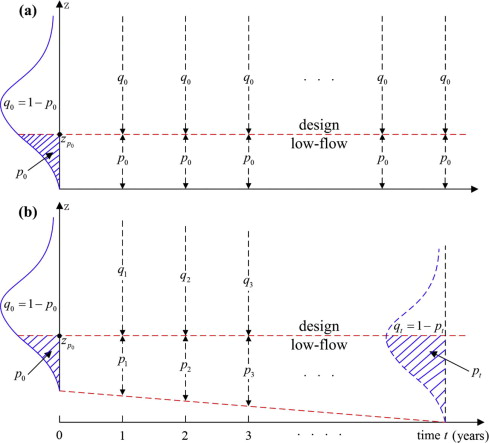
\includegraphics[width=0.8\linewidth]{./work/06-lowflow/figures/Figure_1} 

}

\caption{Schematic depicting the design low-flow quantile $z_{p_{0}}$ with (a) constant exceedance probability $p_{0}$, and (b) time-varying exceedance probabilities $p_{t}, t=1,2, \ldots, \infty$.}(\#fig:fig1\_gamze)
\end{figure}

Source: (\citet{Du2015})

\subsection{Return Period}\label{return-period}

With the method of time-varying moment, deriving a value of a hydrological variable for a return period with a specific design quantile is straightforward (\citet{Olsen1998}; \citet{Villarini2009}). Specifically, \(T_{t}=1 / p_{t}=1 /\left(1-F_{z}\left(z_{p_{0}}, {\theta}_{t}\right)\right)\), where \(T_{t}\) and \(p_{t}\) are the annual return period and exceedance probability, respectively, of the given design quantile \(z_{p_{0}}\) with fitted annual statistical parameters \({\theta}_{t}\), and \(F_{Z}\) is the cumulative distribution function of the hydrological variable of interest. However, for many planning and design applications, a return period measure that varies annually is impractical. To address this issue, various studies have been conducted on return period estimation and risk analysis under nonstationary conditions (\citet{Wigley1988}; \citet{Wigley2009}; \citet{Olsen1998}; \citet{Parey2007}, 2010; \citet{Cooley2013}; \citet{Salas2013}; \citet{Salas2014}). These studies have proposed two different interpretations of return period. The first interpretation is that the expected waiting time (EWT) until the next exceedance event is \(T\) years (\citet{Wigley1988}; \citet{Wigley2009}; \citet{Olsen1998}; \citet{Cooley2013}; \citet{Salas2013}, \citet{Salas2014}). The second interpretation is that the expected number of exceedances (ENE) of the event in \(T\) years is 1 (\citet{Parey2007}, \citet{Parey2010}; \citet{Cooley2013}).

\subsubsection{Return Period Using Expected Waiting Time (EWT) Interpretation}\label{return-period-using-expected-waiting-time-ewt-interpretation}

\textbf{Under stationary conditions}, if \(X\) is the random variable representing the year of the first occurrence of a low-flow that exceeds (i.e., is lower than) the design quantile, then the occurrence of a low-flow \(Z\) exceeding the design value \(z_{p_{0}}\) for the first time in year \(X=x\), \(x=1,2, \ldots, \infty\), follows the geometric probability law (\citet{Mood1974}; \citet{Salas2013}, \citet{Salas2014}):

\[
f(x)=P(X=x)=\left(1-p_{0}\right)^{x-1} p_{0}, \quad x=1,2, \ldots, \infty  \tag{6}
\]

Given that Eq. (3) is based on the assumptions of independence and stationarity, the expected value of \(X\)---representing the return period (expected waiting time interpretation) of the low-flow exceeding the design quantile \(z_{p_{0}}\) under stationary conditions, is:

\[
T=E(X)=\sum_{x=1}^{\infty} x f(x)=1 / p_{0} \tag{7}
\]

\textbf{Under nonstationary conditions}, the exceedance probability associated with \(z_{p_{0}}\) is no longer constant (Fig. 1b). Consequently, the geometric probability law, which takes into account time-varying exceedance probabilities \(p_{t}\), is expressed as (\citet{Cooley2013}, \citet{Salas2013}, \citet{Salas2014}):

\[
\begin{aligned}[b]
f(x) & =P(X=x)=\left(1-p_{1}\right)\left(1-p_{2}\right) \ldots\left(1-p_{x-1}\right) p_{x} \\
& =p_{x} \prod_{t=1}^{x-1}\left(1-p_{t}\right), \quad x=1,2, \ldots, \infty 
\end{aligned}\tag{8}
\]

Therefore, the EWT-return period \(T\) for a low-flow event exceeding the design quantile \(z_{p_{0}}\) under nonstationary conditions is:

\[
 T=E(X)=\sum_{x=1}^{\infty} x f(x)=\sum_{x=1}^{\infty} x p_{x} \prod_{t=1}^{x-1}\left(1-p_{t}\right) \tag{9}
\]

\subsubsection{Return Period Using Expected Number of Exceedances (ENE) Interpretation}\label{return-period-using-expected-number-of-exceedances-ene-interpretation}

\textbf{Under stationary conditions}, if \(M\) is the random variable representing the number of exceedances in \(T\) years, then \(M=\sum_{t=1}^{T} I\left(Z_{t}<z_{p_{0}}\right)\), where \(I(\cdot)\) is the indicator function. In this scenario, \(M\) follows a binomial distribution (\citet{Cooley2013}):

\[
f(m)=P(M=m)=\binom{T}{m} p_{0}^{m}\left(1-p_{0}\right)^{T-m} \tag{10}
\]

It follows that the expected value of \(M\) is 1 :

\[
E(M)=\sum_{t=1}^{T} p_{0}=T p_{0}=1 \tag{11}
\]

Therefore, the return period (expected number of exceedances interpretation) for a low-flow event exceeding the design quantile \(z_{p_{0}}\) under stationary conditions is \(T=1 / p_{0}\).

\textbf{Under nonstationary conditions}, the exceedance probability is not constant, and \(M\) does not follow a binomial distribution. In this context, the expected number of exceedances is expressed as (\citet{Cooley2013}):

\[
\begin{aligned}[b]
E(M) & =\sum_{t=1}^{T} E\left[\left(Z_{t}<z_{p_{0}}\right)\right]=\sum_{t=1}^{T} P\left(Z_{t}<z_{p_{0}}\right)=\sum_{t=1}^{T} F_{Z}\left(z_{p_{0}}, {\theta}_{t}\right) \\
& =\sum_{t=1}^{T} p_{t} 
\end{aligned}\tag{12}
\]

The ENE-return period \(T\) for a low-flow event exceeding the design quantile \(z_{p_{0}}\) under nonstationary conditions can be derived by setting Eq. (12) equal to 1 and solving:

\[
\sum_{t=1}^{T} p_{t}=1 \tag{13} 
\]

\subsection{Hydrological Risk}\label{hydrological-risk}

In practical applications of hydrological frequency analysis, the management question often revolves around risk. Specifically, for a design life of \(n\) years, the hydrological risk \(R\) is defined as the probability of a low-flow event exceeding the design value \(z_{p_{0}}\) before or at year \(n\). This risk can be derived from the complement perspective, meaning there is no exceedance during the design life of \(n\) years.

As an example, consider a low-flow event with a return period of 100 years. The risk for \(t=1\) year is 1\% (i.e., \(R=0.01\)). For \(t=5\) years, the risk increases to approximately 5\%. By \(t=69\) years, the risk reaches 50\%; for \(t=100\) years (the return period), the risk is 63\%; and for \(t=300\) years, the risk climbs to 95\%, and so on (\citet{Wigley2009}).

\textbf{Under the assumptions of independence and stationarity}, the probability of the complement is \(\left(1-p_{0}\right)^{n}\). Consequently, the hydrological risk under stationary conditions is given by (\citet{Haan2002}):

\[
R=1-\left(1-p_{0}\right)^{n} \tag{14}
\]

In recent years, hydrological \textbf{risk analysis under nonstationary conditions} has gained popularity (\citet{Rootzen2013}; \citet{Salas2014}; \citet{Condon2015}; \citet{Serinaldi2015}). This approach offers designers a different perspective from traditional return period and design level methods by incorporating the basic information of design life \(n\) and time-varying exceedance probabilities \(p_{t}\). Similar to the stationary case, for a design life of \(n\) years, the probability of a low-flow event exceeding the design quantile \(z_{p_{0}}\) before or at year \(n\) under time-varying exceedance probabilities \(p_{t}\) is:

\[
R=1-\left[\left(1-p_{1}\right)\left(1-p_{2}\right) \ldots\left(1-p_{n}\right)\right]=1-\prod_{t=1}^{n}\left(1-p_{t}\right) \tag{15}
\]

\textbf{Return Period and Risk Results from Du et al.~(2015)}

\textbf{Nonstationary Return Period Using Meteorological Covariates}

Figure 2 presents the return period and risk results using meteorological covariates (explained in the model selection part) for Huaxian and Xianyang stations.

\begin{itemize}
\item
  \textbf{Panel (a) and (b)}: The black diagonal line represents the stationary case where \(T = T_0\), meaning the return period remains constant over time as expected under stationary assumptions. The other lines depict the nonstationary return periods calculated using the meteorological covariates (temperature and precipitation). These lines show the variability in return periods under nonstationary conditions. The deviations from the diagonal line indicate the impact of changing climatic conditions on the frequency of low-flow events. In nonstationary cases, return periods are generally shorter than the stationary assumption, indicating more frequent low-flow events.
\item
  \textbf{Panel (c) and (d)}: These panels illustrate the nonstationary hydrological risk \(R\) over different design lives (\(n\)). The black solid line shows the stationary risk, providing a baseline for comparison. The nonstationary risk curves, calculated using the covariates, are generally higher than the stationary risk, especially for longer design lives. This indicates a greater likelihood of experiencing low-flow events in the future under nonstationary conditions. The comparison between stationary and nonstationary risks highlights the importance of incorporating nonstationary models in hydrological risk assessments to account for changing climatic conditions.
\end{itemize}

\begin{figure}

{\centering 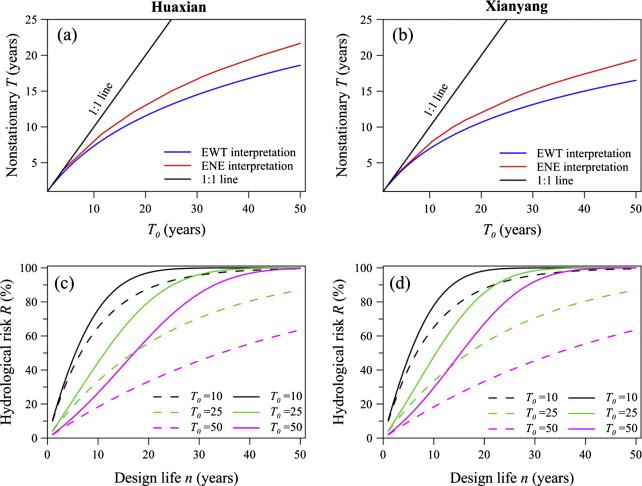
\includegraphics[width=0.8\linewidth]{./work/06-lowflow/figures/Figure_2} 

}

\caption{Nonstationary return period T and hydrological risk R of the Wei River}(\#fig:fig2\_gamze)
\end{figure}

\begin{itemize}
\tightlist
\item
  \textbf{Huaxian Station}:

  \begin{itemize}
  \tightlist
  \item
    \textbf{Expected Waiting Time (EWT)}:

    \begin{itemize}
    \tightlist
    \item
      For a specified initial return period \(T_0 = 50\) years, the nonstationary return period \(T\) was calculated to be 18.6 years.
    \end{itemize}
  \item
    \textbf{Expected Number of Exceedances (ENE)}:

    \begin{itemize}
    \tightlist
    \item
      For \(T_0 = 50\) years, the nonstationary return period \(T\) was calculated to be 22 years.
    \end{itemize}
  \item
    \textbf{Implications}:

    \begin{itemize}
    \tightlist
    \item
      Under nonstationary conditions, the return periods are significantly shorter than the specified \(T_0\), indicating more frequent low-flow events than expected under stationary assumptions.
    \end{itemize}
  \end{itemize}
\item
  \textbf{Xianyang Station}:

  \begin{itemize}
  \tightlist
  \item
    \textbf{Expected Waiting Time (EWT)}:

    \begin{itemize}
    \tightlist
    \item
      Similar to Huaxian, the nonstationary return period \(T\) for \(T_0 = 50\) years was shorter than the specified \(T_0\).
    \end{itemize}
  \item
    \textbf{Expected Number of Exceedances (ENE)}:

    \begin{itemize}
    \tightlist
    \item
      Similar shorter return periods were observed under the ENE interpretation.
    \end{itemize}
  \item
    \textbf{Implications}:

    \begin{itemize}
    \tightlist
    \item
      The results underscore the necessity of accounting for nonstationarity in return period analysis for accurate water resource planning.
    \end{itemize}
  \end{itemize}
\end{itemize}

\textbf{Nonstationary Hydrological Risk Using Meteorological Covariates}

\begin{itemize}
\tightlist
\item
  \textbf{Huaxian Station}:

  \begin{itemize}
  \tightlist
  \item
    \textbf{Risk Calculations}:

    \begin{itemize}
    \tightlist
    \item
      For a design life \(n\) of 10 years and \(T_0 = 50\) years, the hydrological risk \(R\) was 14.1\% under nonstationary conditions, compared to 18.3\% under stationary conditions.
    \item
      For \(n = 40\) years and \(T_0 = 50\) years, the risk \(R\) was 79.0\% under nonstationary conditions, significantly higher than the stationary risk of 55.4\%.
    \end{itemize}
  \item
    \textbf{Implications}:

    \begin{itemize}
    \tightlist
    \item
      The nonstationary risk is higher, especially for longer design lives, indicating an increased likelihood of low-flow events over time.
    \end{itemize}
  \end{itemize}
\item
  \textbf{Xianyang Station}:

  \begin{itemize}
  \tightlist
  \item
    \textbf{Risk Calculations}:

    \begin{itemize}
    \tightlist
    \item
      For \(n = 10\) years and \(T_0 = 50\) years, the risk \(R\) was 5.8\% under nonstationary conditions.
    \item
      For \(n = 40\) years and \(T_0 = 50\) years, the risk \(R\) was 68.4\% under nonstationary conditions.
    \end{itemize}
  \item
    \textbf{Implications}:

    \begin{itemize}
    \tightlist
    \item
      Similar to Huaxian, the nonstationary risk for Xianyang is significantly higher, emphasizing the impact of nonstationarity on hydrological risk assessments.
    \end{itemize}
  \end{itemize}
\end{itemize}

\subsection{Nonstationary frequency analysis of low-flow series}\label{nonstationary-frequency-analysis-of-low-flow-series}

The standard method for calculating nonstationary return periods under the EWT and ENE interpretations, as well as the risk of a design quantile \(z_{p_{0}}\) corresponding to an initial return period \(T_{0}\), is outlined by Eqs. (9), (13), (15), respectively. A crucial aspect of this procedure is the derivation of time-varying exceedance probabilities \(p_{t}\) (Eq. (5)) for future years. This process involves determining the relationships between the statistical parameters of the low-flow distribution and the explanatory variables, which is typically referred to as nonstationary frequency analysis.

\subsubsection{GAMLSS}\label{gamlss}

The nonstationary low-flow series is modeled using the Generalized Additive Models in Location, Scale, and Shape (GAMLSS) framework (\citet{Rigby2005}). The GAMLSS framework assumes that independent observations \(z_{i}\) for \(i = 1, 2, 3, \ldots, n\) have a distribution function \(f(z_{i} \mid \theta^{i})\), where \(\theta^{i} = (\theta_{1}^{i}, \theta_{2}^{i}, \ldots, \theta_{p}^{i})\) is a vector of \(p\) distribution parameters accounting for the location, scale, and shape of the random variable characteristics. Usually, \(p\) is less than or equal to four, since the 1-, 2-, 3-, and 4-parameter families ensure sufficient flexibility for most applications in hydrology.

Given an \(n\)-length vector of the response variable \(z^{T} = (z_{1}, \ldots, z_{n})\), let \(g_{k}(\cdot)\), for \(k = 1, 2, \ldots, p\), be known monotonic link functions relating the distribution parameters to explanatory variables and random effects through an additive model given by:

\[
g_{k}(\theta_{k}) = \eta_{k} = X_{k} \beta_{k} + \sum_{j=1}^{J_{k}} Z_{jk} \gamma_{jk}\tag{16}
\]

where \(\eta_{k}\) and \(\theta_{k}\) are vectors of length \(n\) (e.g., \(\theta_{k}^{T} = (\theta_{k}^{1}, \theta_{k}^{2}, \ldots, \theta_{k}^{n})\)), \(\beta_{k}^{T} = (\beta_{1k}, \beta_{2k}, \ldots, \beta_{Jkk})\) is a parameter vector of length \(J_{k}\), \(\mathbf{X}_{k}\) is a matrix of explanatory variables (i.e., covariates) of order \(n \times J_{k}\), \(Z_{jk}\) is a fixed known \(n \times q_{jk}\) design matrix, and \(\gamma_{jk}\) is a \(q_{jk}\)-dimensional random variable. The linear predictors \(\eta_{k}\) for \(k = 1, \ldots, p\) comprise a parametric component \(\mathbf{X}_{k} \beta_{k}\) (linear functions of explanatory variables) and the additive component \(Z_{jk} \gamma_{jk}\) (linear functions of stochastic variables). If \(Z_{jk} = \mathrm{I}_{n}\), where \(\mathrm{I}_{n}\) is an \(n \times n\) identity matrix and \(\gamma_{jk} = h_{jk} = h_{jk}(x_{jk})\) for all combinations of \(j\) and \(k\), we obtain the semi-parametric additive formulation of GAMLSS:

\[
g_{k}(\theta_{k}) = \eta_{k} = X_{k} \beta_{k} + \sum_{j=1}^{J_{k}} h_{jk}(x_{jk})\tag{17}
\]

where \(\theta_{k}\) is the parameter vector of length \(n\), \(\mathbf{X}_{jk}\) is a matrix of explanatory variables of order \(n \times m\), \(\beta_{k}\) is a parameter vector of length \(m\), and \(h_{jk}\) denotes the functional dependence of the distribution parameters on explanatory variables \(x_{jk}\), which is a column of matrix \(\mathbf{X}_{jk}\). This dependence can be linear or smoothed using smoothing terms, and the smooth dependence is based on a cubic spline function (\citet{Lopez2013}).

Various probability distributions have been suggested for modeling low-flow events (\citet{Matalas1963}; \citet{Eratakulan1970}; \citet{Smakhtin2001}; \citet{Hewa2007}; \citet{Liu2015}). Matalas (1963) investigated four distributions in modeling low-flow data from 34 streams and found that the Gumbel and Pearson-III distributions fit the data well and were more representative than the Lognormal and Pearson-V distributions. Eratakulan (1970) discovered that the Gamma and Weibull distributions were the most suitable for modeling the low-flow series from 37 stations in the Missouri River basin. Hewa et al.~(2007) introduced the GEV distribution into the frequency analysis of low-flow data from 97 catchments in Victoria, Australia. Liu et al.~(2015) tested six distributions for modeling the annual low flows at the Yichang station, China, under nonstationary conditions and found that the GEV distribution provided the best fit.

Based on these studies, five two-parameter distributions (Gamma (GA), Weibull (WEI), Gumbel (GU), Logistic (LO), and Lognormal (LOGNO)) and two three-parameter distributions (Pearson-III (P-III) and GEV) that are widely used in modeling low-flow data are listed in Table 1. Considering that the shape parameter \(\kappa\) of the P-III and GEV distributions is quite sensitive and difficult to estimate, it is mostly assumed to be constant (\citet{Coles2001}; \citet{Katz2002}; \citet{Gilroy2012}; \citet{Du2015}). Nonstationarities in both the location \(\mu\) and scale \(\sigma\) parameters are examined through monotonic link functions \(\mathrm{g}(\cdot)\).

\begin{longtable}[]{@{}
  >{\raggedright\arraybackslash}p{(\columnwidth - 6\tabcolsep) * \real{0.0216}}
  >{\raggedright\arraybackslash}p{(\columnwidth - 6\tabcolsep) * \real{0.5669}}
  >{\raggedright\arraybackslash}p{(\columnwidth - 6\tabcolsep) * \real{0.2748}}
  >{\raggedright\arraybackslash}p{(\columnwidth - 6\tabcolsep) * \real{0.1338}}@{}}
\toprule\noalign{}
\begin{minipage}[b]{\linewidth}\raggedright
Distribution
\end{minipage} & \begin{minipage}[b]{\linewidth}\raggedright
Probability Density Function
\end{minipage} & \begin{minipage}[b]{\linewidth}\raggedright
Moments
\end{minipage} & \begin{minipage}[b]{\linewidth}\raggedright
Link Functions
\end{minipage} \\
\midrule\noalign{}
\endhead
\bottomrule\noalign{}
\endlastfoot
Gamma & \(f_{Z}(z \mid \mu, \sigma) = \frac{1}{(\mu \sigma^{2})^{1 / \sigma^{2}}} \frac{z^{(1 / \sigma^{2} - 1) e^{-z(\mu \sigma^{2})}}}{\Gamma(1 / \sigma^{2})}\) \(z > 0, \mu > 0, \sigma > 0\) & \(E(Z) = \mu\) \(SD(Z) = \mu \sigma\) & \(g_{1}(\mu) = \ln (\mu)\) \(g_{2}(\sigma) = \ln (\sigma)\) \\
Weibull & \(f_{Z}(z \mid \mu, \sigma) = \frac{\sigma z^{\sigma - 1}}{\mu^{\sigma}} \exp \left[-\left(\frac{z}{\mu}\right)^{\sigma}\right]\) \(z > 0, \mu > 0, \sigma > 0\) & \(E(Z) = \mu \Gamma \left( \frac{1}{\sigma} + 1 \right)\) \(SD(Z) = \mu \sqrt{\Gamma \left( \frac{2}{\sigma} + 1 \right) - \left[ \Gamma \left( \frac{1}{\sigma} + 1 \right) \right]^{2}}\) & \(g_{1}(\mu) = \ln (\mu)\) \(g_{2}(\sigma) = \ln (\sigma)\) \\
Gumbel & \(f_{Z}(z \mid \mu, \sigma) = \frac{1}{\sigma} \exp \left\{ -\left( \frac{z - \mu}{\sigma} \right) - \exp \left[ -\left( \frac{z - \mu}{\sigma} \right) \right] \right\}\) \(-\infty < z < \infty, -\infty < \mu < \infty, \sigma > 0\) & \(E(Z) = \mu + \gamma \sigma \simeq \mu + 0.57722 \sigma\) \(SD(Z) = \frac{\pi}{\sqrt{6}} \sigma \simeq 1.28255 \sigma\) & \(g_{1}(\mu) = \mu\) \(g_{2}(\sigma) = \ln (\sigma)\) \\
Logistic & \(f_{Z}(z \mid \mu, \sigma) = \frac{1}{\sigma} \left\{ \exp \left[ -\left( \frac{z - \mu}{\sigma} \right) \right] \right\} \left\{ 1 + \exp \left[ -\left( \frac{z - \mu}{\sigma} \right) \right] \right\}^{-2}\) \(-\infty < z < \infty, -\infty < \mu < \infty, \sigma > 0\) & \(E(Z) = \mu\) \(SD(Z) = \frac{\pi}{\sqrt{3}} \sigma \simeq 1.81380 \sigma\) & \(g_{1}(\mu) = \mu\) \(g_{2}(\sigma) = \ln (\sigma)\) \\
Lognormal & \(f_{Z}(z \mid \mu, \sigma) = \frac{1}{\sqrt{2 \pi}} \frac{1}{z} \exp \left\{ -\frac{(\log(z) - \mu)^{2}}{2 \sigma^{2}} \right\}\) \(z > 0, \mu > 0, \sigma > 0\) & \(E(Z) = w^{1 / 2} e^{\mu}\) \(SD(Z) = \sqrt{w(w - 1)} e^{\mu}\) \(w = \exp (\sigma^{2})\) & \(g_{1}(\mu) = \mu\) \(g_{2}(\sigma) = \ln (\sigma)\) \\
Pearson-III & \(f_{Z}(z \mid \mu, \sigma, \kappa) = \frac{1}{\sigma \mu \kappa \Gamma \left(1 / \kappa^{2}\right)} \left( \frac{z - \mu}{\mu \sigma \kappa} + \frac{1}{\kappa^{2}} \right)^{\frac{1}{\kappa^{2}} - 1} \exp \left[ -\left( \frac{z - \mu}{\mu \sigma \kappa} + \frac{1}{\kappa^{2}} \right) \right\}\) \(\sigma > 0, \kappa \neq 0, \frac{z - \mu}{\mu \sigma \kappa} + \frac{1}{\kappa^{2}} \geq 0\) & \(E(Z) = \mu\) \(Cv = \sigma\) \(Cs = 2 \kappa\) & \(g_{1}(\mu) = \ln (\mu)\) \(g_{2}(\sigma) = \ln (\sigma)\) \(g_{3}(\kappa) = \kappa\) \\
GEV & \(f_{Z}(z \mid \mu, \sigma, \kappa) = \frac{1}{\sigma} \left[1 + \kappa \left( \frac{z - \mu}{\sigma} \right)\right]^{(-1 / \kappa) - 1} \exp \left\{ -\left[ 1 + \kappa \left( \frac{z - \mu}{\sigma} \right) \right]^{-1 / \kappa} \right\}\) \(-\infty < \mu < \infty, \sigma > 0, -\infty < \kappa < \infty\) & \(E(Z) = \mu - \frac{\sigma}{\kappa} + \frac{\sigma}{\kappa} \eta_{1}\) \(SD(Z) = \sigma \sqrt{\eta_{2} - \eta_{1}^{2}} / \kappa\) \(\eta_{m} = \Gamma(1 - m \kappa)\) & \(g_{1}(\mu) = \mu\) \(g_{2}(\sigma) = \ln (\sigma)\) \(g_{3}(\kappa) = \kappa\) \\
\end{longtable}

\textbf{Table 1: Summary of the distributions used to model the low-flow series (\citet{Du2015})}

\subsubsection{Model Selection}\label{model-selection}

The optimal nonstationary model was selected by penalizing more complex models using the Akaike Information Criterion (AIC) (\citet{Akaike1974}) and the Bayesian Information Criterion (BIC) (\citet{Schwarz1978}). The AIC is calculated as:

\[
\mathrm{AIC}=-2 \ln (\mathrm{ML})+2 k \tag{18}
\]

where ML is the maximum likelihood function of the models and \(k\) is the number of independently adjusted parameters within the model. Theoretically, \(-\infty < \mathrm{AIC} < \infty\). Similarly, BIC is calculated as:

\[
\mathrm{BIC}=-2 \ln (\mathrm{ML})+k \ln(n) \tag{19}
\]

where \(n\) is the number of observations. The model with the smallest AIC and BIC values is considered the optimal one.

\subsubsection{Goodness-of-fit}\label{goodness-of-fit}

While the information criterion value identifies the optimal model, it is not a measure of model performance. The goodness-of-fit of the selected optimal model was assessed qualitatively using the worm plots (Buuren and Fredriks, 2001) and centile curves diagnostic plots, and quantitatively using the statistics of the Filliben correlation coefficient (denoted by \(F_{r}\)) (\citet{Filliben1975}) and the Kolmogorov-Smirnov (KS) test (denoted by \(\left.D_{KS}\right)\) (\citet{Massey1951}). \(F_{r}\) and \(\left.D_{KS}\right)\) are calculated by Eqs. (20) and (22), respectively:

\[
F_{r}=\operatorname{Cor}(S, B)=\frac{\sum_{i=1}^{\tau}\left(S_{(i)}-\bar{S}\right)\left(B_{i}-\bar{B}\right)}{\sqrt{\sum_{i=1}^{\tau}\left(S_{(i)}-\bar{S}\right)^{2} \sum_{i=1}^{\tau}\left(B_{i}-\bar{B}\right)^{2}}} \tag{20}
\]

where \(S_{(i)}\) are the ordered residuals obtained by sorting \(\Phi^{-1}\left[F_{Z}\left(z_{i}, {\theta}{i}\right)\right]\) in ascending order for \(1 \leqslant i \leqslant \tau\). Here, \(\Phi^{-1}\) denotes the inverse function of the standard normal distribution, and \(\tau\) represents the length of the observation period (similarly hereinafter). \(B{i}\) are the standard normal order statistic medians calculated from \(\Phi^{-1}\left(b_{i}\right)\), where \(b_{i}\) are derived by:

\[
b_{i}=\left\{\begin{array}{lc}1-b_{\tau} & i=1 \\ (i-0.3175) /(\tau+0.365) & i=2,3, \ldots, \tau-1 \\ 0.5^{(1 / \tau)} & i=\tau\end{array}\right.\tag{21}
\]

\(F_{r}\) ranges from \((0,1]\), and an \(F_{r}\) value greater than the critical value \(F_{\alpha}\) indicates that the nonstationary model passes the goodness-of-fit test.

\[
D_{K S}=\max _{1 \leq i \leq \tau}\left|\hat{G}_{i}-G_{(i)}\right| \tag{22}
\]

where \(\hat{G}{i}\) are the empirical cumulative probabilities calculated as \(i /(\tau+1)\), and \(G{(i)}\) are the ordered theoretical cumulative probabilities obtained by sorting \(F_{Z}\left(z_{i}, {\theta}{i}\right)\) in ascending order for \(1 \leqslant i \leqslant \tau\). \(D{KS}\) ranges from \([0,1]\), and a \(D_{KS}\) value smaller than the critical value \(D_{\alpha}\) indicates that the nonstationary model passes the goodness-of-fit test.

To summarize, the main steps in deriving time-varying exceedance probabilities \(p_{t}\) for future years are:

\begin{enumerate}
\def\labelenumi{(\roman{enumi})}
\item
  Nonstationary modeling of the observed low-flow series using either time alone or meteorological variables as covariates.
\item
  Calculating the design low-flow quantile \(z_{p_{0}}\) corresponding to an initial return period \(T_{0}\) from the quantile function \(z_{p_{0}}=F_{Z}^{-1}\left(p_{0}, {\theta}_{0}\right)\), where \(p_{0}=1 / T_{0}\) and \({\theta}_{0}\) is the fitted statistical parameter set of the initial year \(t=0\).
\item
  Deriving time-varying exceedance probabilities \(p_{t}\) corresponding to \(z_{p_{0}}\) for future years \(t=1,2, \ldots, \infty\) (when using time as a covariate) or \(t=1,2, \ldots, t_{\max }\) (when using meteorological covariates) from Eq. (5) where \({\theta}_{t}\) is calculated by extending the optimal nonstationary model from step (i) into the future under the respective case of covariates.
\end{enumerate}

\textbf{Applications of Model Selection and Goodness of Fit}

This table summarizes the model selection and goodness of fit for low flow series as analyzed in three different studies. Each study applied various statistical criteria to select the best-fit models for different hydrological stations. The goodness of fit measures include diagnostic tools like Worm plots, Kolmogorov-Smirnov test, and others. The selected distributions and their parameters are highlighted for each station.

\begin{longtable}[]{@{}
  >{\raggedright\arraybackslash}p{(\columnwidth - 8\tabcolsep) * \real{0.0528}}
  >{\raggedright\arraybackslash}p{(\columnwidth - 8\tabcolsep) * \real{0.0691}}
  >{\raggedright\arraybackslash}p{(\columnwidth - 8\tabcolsep) * \real{0.0549}}
  >{\raggedright\arraybackslash}p{(\columnwidth - 8\tabcolsep) * \real{0.1789}}
  >{\raggedright\arraybackslash}p{(\columnwidth - 8\tabcolsep) * \real{0.6382}}@{}}
\toprule\noalign{}
\begin{minipage}[b]{\linewidth}\raggedright
Study
\end{minipage} & \begin{minipage}[b]{\linewidth}\raggedright
Selected Model for Each Station
\end{minipage} & \begin{minipage}[b]{\linewidth}\raggedright
Model Selection Criteria
\end{minipage} & \begin{minipage}[b]{\linewidth}\raggedright
Goodness of Fit
\end{minipage} & \begin{minipage}[b]{\linewidth}\raggedright
Selected Distribution with Parameters
\end{minipage} \\
\midrule\noalign{}
\endhead
\bottomrule\noalign{}
\endlastfoot
\textbf{Du et al.~(2015)} & Huaxian: Weibull

Xianyang: Gamma & AIC & Worm plots, Centile curves, Filliben Correlation Coefficient, Kolmogorov-Smirnov test & \(\text{Huaxian}\): \(\ln(\mu) \sim \text{Temp}\), \(\ln(\sigma) \sim \text{Pr}\) \(\text{Xianyang}\): \(\ln(\mu) \sim \text{Temp}\), \(\ln(\sigma) \sim \text{constant}\) \\
\textbf{Wang et al.~(2022)} & DPL: Weibull

CTG: Weibull

ZGP: Weibull

XX: Weibull & AIC & Worm plots, Kolmogorov-Smirnov test & \(\text{DPL}\): \(\mu \sim \text{cs(Pr, 2)}\), \(\sigma \sim \text{constant}\) \(\text{CTG}\): \(\mu \sim \text{cs(Pr, 3)}\), \(\sigma \sim \text{constant}\) \(\text{ZGP}\): \(\mu \sim \text{cs(Pr, 2)} + \text{RI}\), \(\sigma \sim \text{RI}\) \(\text{XX}\): \(\mu \sim \text{cs(Pr, 2)}\), \(\sigma \sim \text{constant}\) \\
\textbf{Jiang et al.~(2015)} & Qa: Gamma

Qh: Gamma & AICc & Worm plots, Kolmogorov-Smirnov test & \(\text{Qa}\): \(\mu \sim \text{constant}\), \(\sigma \sim \ln(\text{RI}_a)\) \(\text{Qh}\): \(\mu \sim \ln(\text{RI}_h)\), \(\sigma \sim \text{constant}\) \\
\end{longtable}

\begin{itemize}
\tightlist
\item
  \textbf{Du et al.~(2015)}:

  \begin{itemize}
  \tightlist
  \item
    \textbf{Huaxian Station}: Selected Weibull distribution with temperature (Temp) and precipitation (Pr) as covariates.
  \item
    \textbf{Xianyang Station}: Selected Gamma distribution with temperature and a constant scale parameter.
  \end{itemize}
\item
  \textbf{Wang et al.~(2022)}:

  \begin{itemize}
  \tightlist
  \item
    Selected Weibull distribution for \textbf{DPL, CTG, ZGP}, and \textbf{XX} stations with various covariates. Precipitation was modeled using cubic splines (cs) and reservoir index (RI) was included for some stations.
  \end{itemize}
\item
  \textbf{Jiang et al.~(2015)}:

  \begin{itemize}
  \tightlist
  \item
    Selected Gamma distribution for \textbf{Qa} and \textbf{Qh} low-flow series of the respective stations with reservoir index as covariate.
  \end{itemize}
\end{itemize}

These results underscore the importance of incorporating climatic variables (e.g., temperature and precipitation) and anthropogenic factors (e.g., reservoir index) into nonstationary models to better capture the variability and trends in low flow series. The use of cubic splines to model non-linear relationships and the selection of appropriate distributions based on AIC and other diagnostic tools (e.g., worm plots, Filliben correlation coefficient) ensure that the models are well-fitted to the observed data, thereby providing robust tools for hydrological analysis and water resource management.

\section{Bivariate Statistical Analysis}\label{bivariate-statistical-analysis}

Bivariate statistical analysis is an essential tool in hydrology, providing insights into the interactions between different hydrological variables, especially during low-flow events. Unlike univariate analysis, which examines a single variable in isolation, bivariate analysis allows us to explore the joint behavior of two variables, offering a more comprehensive understanding of hydrological phenomena.

One of the advanced methodologies in this domain is the use of copulas, which enable the modeling of dependencies between variables without the restrictive assumptions of linearity or normality. Copulas provide a flexible framework to construct joint distributions, capturing the dependence structure between variables more accurately.

Given the dynamic nature of hydrological processes influenced by climate change and human activities such as reservoir operations, it is crucial to account for nonstationarity in these analyses. This is where time-varying copulas come into play. Unlike static copulas, time-varying copulas allow the parameters defining the dependence structure to evolve over time, reflecting the changing environmental conditions.

In this context, the content that will be presented here is heavily based on the methodologies and findings from the study ``Bivariate frequency analysis of nonstationary low-flow series based on the time-varying copula'' by Jiang et al (2015). This study exemplifies how time-varying copulas can effectively model the joint distribution of low-flow events under nonstationary conditions, taking into account both the marginal distributions and the evolving dependence structure.

\subsection{Joint Return Period Under Nonstationary Framework}\label{joint-return-period-under-nonstationary-framework}

Three methods have been used to calculate the joint return period (JPR) of low-flow events in stationary bivariate frequency analysis: the AND method, corresponding to the probability \(P(Y_{1} \leq y_{1} \wedge Y_{2} \leq y_{2})\); the OR method, corresponding to the probability \(P(Y_{1} \leq y_{1} \vee Y_{2} \leq y_{2})\); and the Kendall (KEN) return period method. The Kendall return period, a multivariate return period first defined by Salvadori and De Michele (2004b), has been widely applied in analyzing the joint return periods of floods or droughts (\citet{Salvadori2007}, \citet{Salvadori2010}, \citet{Salvadori2011}, \citet{DeMichele2013}, \citet{Graler2013}, \citet{Salvadori2013}). The JPR using the KEN method for low-flow events is given by:

\[
\begin{aligned}[b]
T_{KEN} &= \frac{\lambda}{P\left[C\left(u_{1}, u_{2} \mid \theta_{c}\right) \leq p_{KEN}\right]} \\
&= \frac{\lambda}{P\left\{C\left[F_{1}\left(y_{1} \mid \boldsymbol{\theta}_{1}\right), F_{2}\left(y_{2} \mid \boldsymbol{\theta}_{2}\right) \mid \theta_{c}\right] < p_{KEN}\right\}}  \\
&= \frac{\lambda}{K_{C}\left(p_{KEN}\right)}
\end{aligned}\tag{23}
\]

where \(\lambda\) is the average interarrival time between low-flow event occurrences. In this paper, the annual minimum low-flow series is investigated, so \(\lambda\) is set to 1 (i.e., \(\lambda = 1\)). \(K_{C}(\cdot)\) is the Kendall distribution function (\citet{Genest1993}, \citet{Barbe1996}, \citet{Salvadori2007}), which provides a univariate representation of multivariate information, and \(p_{KEN}\) is a critical probability level corresponding to the value of \(K_{C}(p_{KEN})\) (\citet{Salvadori2011}, \citet{Salvadori2013}).

Similar to calculating the JPR of low-flow events in stationary bivariate frequency analysis, the JPRs for AND, OR, and KEN methods in nonstationary circumstances are defined as follows:

\[
\begin{aligned}
T_{A N D}^{t}=\frac{1}{P\left(Y_{1} \leq y_{1} \wedge Y_{2} \leq y_{2}\right)}\\
=\frac{1}{C\left[F_{1}\left(y_{1} \mid \boldsymbol{\theta}_{1}^{t}\right), F_{2}\left(y_{2} \mid \boldsymbol{\theta}_{2}^{t}\right) \mid \theta_{c}^{t}\right]} \\
T_{O R}^{t}=\frac{1}{P\left(Y_{1} \leq y_{1} \vee Y_{2} \leq y_{2}\right)} \\
=\frac{1}{P\left(Y_{1} \leq y_{1}\right)+P\left(Y_{2} \leq y_{2}\right)-P\left(Y_{1} \leq y_{1} \wedge Y_{2} \leq y_{2}\right)} \\
=\frac{1}{F_{1}\left(y_{1} \mid \boldsymbol{\theta}_{1}^{t}\right)+F_{2}\left(y_{2} \mid \boldsymbol{\theta}_{2}^{t}\right)-C\left[F_{1}\left(y_{1} \mid \boldsymbol{\theta}_{1}^{t}\right), F_{2}\left(y_{2} \mid \boldsymbol{\theta}_{2}^{t}\right) \mid \theta_{c}^{t}\right]} 
\end{aligned}\tag{24}
\]

\[
T_{K E N}^{t}=\frac{1}{P\left[C\left(u_{1}^{t}, u_{2}^{t} \mid \theta_{c}^{t}\right) \leq p_{K E N}\right]}
\]

\[
=\frac{1}{P\left\{C\left[F_{1}\left(y_{1} \mid \boldsymbol{\theta}_{1}^{t}\right), F_{2}\left(y_{2} \mid \boldsymbol{\theta}_{2}^{t}\right) \mid \theta_{c}^{t}\right]<p_{K E N}\right\}} \tag{25}
\]

\[
=\frac{1}{K_{C}^{t}\left(p_{K E N}\right)}
\]

\textbf{Joint Return Period in Jiang et al.~(2015)}

Jiang et al.~(2015) analyzed the joint return period of low-flow events at the Ankang (Qa) and Huangzhuang (Qh) gauges on the Hanjiang River using a time-varying copula model. The study used three methods to calculate the JRP: AND, OR, and Kendall (KEN) methods.

\textbf{Time Variation in the Joint Return Periods}:

\begin{itemize}
\tightlist
\item
  \textbf{1954--1967}: Before major reservoirs were built.
\item
  \textbf{1968--1991}: After the Danjiangkou Reservoir was operational.
\item
  \textbf{1992--2011}: After the Ankang Reservoir was operational.
\end{itemize}

The JRP isolines of the design low-flow pairs for a given JRP of 50 years were calculated for each time segment. The study found that reservoir operations significantly impacted the joint distribution and return periods of low flows at both gauges.

\textbf{Results}:

\begin{figure}

{\centering 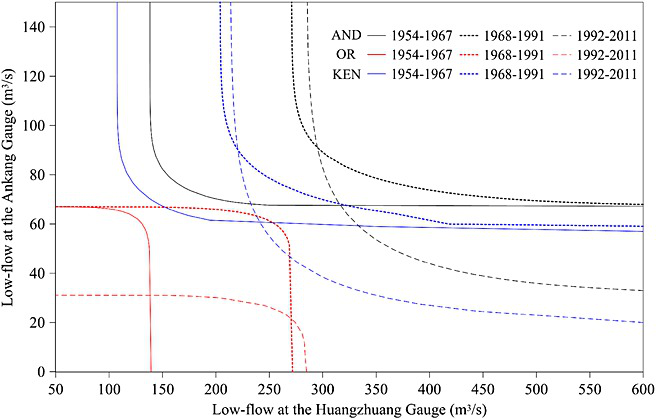
\includegraphics[width=0.8\linewidth]{./work/06-lowflow/figures/Figure_3} 

}

\caption{The isolines of design low-flow events with JRP=50 years for three different time periods of 1954-1967, 1968-1991 and 1992-2011}(\#fig:fig3\_gamze)
\end{figure}

\begin{itemize}
\tightlist
\item
  \textbf{AND Method}: The JRP isoline moved horizontally to the right from 1954--1967 to 1968--1991 due to the increased mean of Huangzhuang low flow. It then moved downward from 1968--1991 to 1992--2011 due to the increased coefficient of variation of Ankang low flow.
\item
  \textbf{OR and KEN Methods}: Showed similar variations to the AND method.
\end{itemize}

\textbf{Implications}:

\begin{itemize}
\tightlist
\item
  The movement of JRP isolines indicates the significant influence of reservoir operations on the hydrological regime. Specifically, the changes in JRP isolines reflect how human activities, such as the construction and operation of reservoirs, alter the dependence structure between low-flow events at different gauges.
\item
  The results highlight the necessity of considering nonstationarity in hydrological frequency analysis to accurately assess the impacts of climate variability and human interventions on water resources.
\end{itemize}

These findings emphasize the importance of integrating nonstationary models and anthropogenic factors in hydrological studies to improve the reliability of low-flow frequency analysis and water resource management.

\subsection{Time-Varying Copula Model}\label{time-varying-copula-model}

Based on the definition of the copula (\citet{nelsen2006}, \citet{Salvadori2007}) the time-varying copula can be expressed as:

\[
\begin{aligned}[b]
H_{Y_{1}, Y_{2}}\left(y_{1}^{t}, y_{2}^{t}\right) & =C\left[F_{1}\left(y_{1}^{t} \mid \boldsymbol{\theta}_{1}^{t}\right), F_{2}\left(y_{2}^{t} \mid \boldsymbol{\theta}_{2}^{t}\right) \mid \theta_{c}^{t}\right]  \\
& =C\left(u_{1}^{t}, u_{2}^{t} \mid \theta_{c}^{t}\right)
\end{aligned}\tag{26}
\]

where \(C(\cdot)\) denotes the copula function, \(F(\cdot)\) is the cumulative distribution function, \(\boldsymbol{\theta}_{1}^{t}\) and \(\boldsymbol{\theta}_{2}^{t}\) represent the time-varying marginal distribution parameters, and \(\theta_{c}^{t}\) is the time-varying copula parameter. Additionally, the marginal probabilities \(u_{1}^{t}\) and \(u_{2}^{t}\) within the time-varying copula must both follow a uniform distribution over the interval \([0,1]\).

According to Equation (27), three scenarios for the time-varying copula can be derived:

\begin{itemize}
\item
  all the marginal distribution parameters are constant while the copula parameter is time-varying,
\item
  at least one marginal distribution parameter is time-varying while the copula parameter remains constant, and
\item
  both at least one marginal distribution parameter and the copula parameter are time-varying.
\end{itemize}

The implementation of the time-varying copula model in Equation (27) involves two major steps: first, determining the time variation in the marginal distributions, and second, modeling the evolution of the copula parameter. The first step is done under the GAMLSS framework we have discussed before. As the second step the copula parameter \(\theta_{c}\) can be expressed as a linear function of the time-varying explanatory variables \(x_{i}^{t} (i=1,2, \ldots, m)\) through a suitable link function \(g_{c}(\cdot)\), as follows:

\[
g_{c}\left(\theta_{c}^{t}\right) = \beta_{0} + \sum_{i=1}^{m} \beta_{i} x_{i}^{t} \tag{27}
\]

where \(\beta_{0}, \beta_{1}, \ldots, \beta_{m}\) are the parameters represented by the vector \(\boldsymbol{\beta} = \left(\beta_{0}, \beta_{1}, \ldots, \beta_{m}\right)^{\mathrm{T}}\). The link function \(g_{c}(\cdot)\) depends on the domain of the copula parameter. For example, if \(\theta_{c} \in \mathbb{R}\), then \(g_{c}(\theta_{c}) = \theta_{c}\) (for the Frank copula), or if \(\theta_{c} > 0\), then \(g_{c}(\theta_{c}) = \log(\theta_{c})\) (for the GH and Clayton copulas). The time-varying copula parameters \(\boldsymbol{\beta}_{i}\) are estimated by Inference Function for Margins (IFM) method (\citet{Joe1997}).

\subsection{Model Selection and Goodness-of-fit}\label{model-selection-and-goodness-of-fit}

Model selection in terms of copula functions involves evaluating different copula models to determine which best fits the data. Similar to bivariate analysis, criteria such as the Akaike Information Criterion (AIC) and the Bayesian Information Criterion (BIC) are commonly used for this purpose. Additionally, variations like the corrected Akaike Information Criterion (AICc) can be employed, especially when dealing with smaller sample sizes. By comparing the AIC, BIC, or AICc values of various copula models, the model with the lowest criterion value is chosen, indicating the best trade-off between model complexity and goodness of fit.

The goodness-of-fit of the time-varying copula model is evaluated by assessing the fit of both the two marginal distributions and the copula function. The goodness-of-fit test for the copula is conducted using Rosenblatt's probability integral transform (\citet{Rosenblatt1952}, \citet{Genest2009}).

\textbf{Chosen Copula Models and AICc Values in Jiang et al.~(2015)}

The study by Jiang et al.~(2015) focused on analyzing the time-varying dependence structure between the low-flow series at the Ankang (Qa) and Huangzhuang (Qh) gauges. The authors selected three Archimedean copulas (Frank, Gumbel-Hougaard (GH), and Clayton) due to their flexibility and ability to capture different dependence structures. The models were evaluated using two different explanatory variables: time and reservoir index (RI). The selection criteria include the corrected Akaike Information Criterion (AICc), which is preferred over the regular AIC when dealing with small sample sizes as it adjusts for the number of parameters in the model, providing a more accurate measure of model fit.

\textbf{With Time as the Explanatory Variable}

\begin{longtable}[]{@{}ccc@{}}
\toprule\noalign{}
Copula Type & Copula Parameter Model & AICc \\
\midrule\noalign{}
\endhead
\bottomrule\noalign{}
\endlastfoot
Frank & \(\theta(t) = 7.580 + 0.091t\) & -29.41 \\
GH & \(\theta(t) = \exp(0.772 + 0.007t)\) & -27.50 \\
Clayton & \(\theta(t) = \exp(0.442 + 0.022t)\) & -14.33 \\
\end{longtable}

\textbf{With Reservoir Index as the Explanatory Variable}

\begin{longtable}[]{@{}
  >{\centering\arraybackslash}p{(\columnwidth - 4\tabcolsep) * \real{0.1647}}
  >{\centering\arraybackslash}p{(\columnwidth - 4\tabcolsep) * \real{0.6706}}
  >{\centering\arraybackslash}p{(\columnwidth - 4\tabcolsep) * \real{0.1529}}@{}}
\toprule\noalign{}
\begin{minipage}[b]{\linewidth}\centering
Copula Type
\end{minipage} & \begin{minipage}[b]{\linewidth}\centering
Copula Parameter Model
\end{minipage} & \begin{minipage}[b]{\linewidth}\centering
AICc
\end{minipage} \\
\midrule\noalign{}
\endhead
\bottomrule\noalign{}
\endlastfoot
Frank & \(\theta(\text{RI}_h) = 9.096 - 9.753\text{RI}_h\) & -31.10 \\
GH & \(\theta(\text{RI}_h) = \exp(0.970 - 0.946\text{RI}_h)\) & -30.16 \\
Clayton & \(\theta(\text{RI}_h) = \exp(0.461 - 1.681\text{RI}_h)\) & -14.61 \\
\end{longtable}

The tables shows that the Frank copula with the reservoir index (RI) as the explanatory variable had the lowest AICc value of -31.10, indicating the best fit among the evaluated models. This is followed by the GH copula with an AICc of -30.16, and the Clayton copula with an AICc of -14.61. In comparison, when time was used as the explanatory variable, the Frank copula still performed best with an AICc of -29.41, but its fit was not as good as with the reservoir index.

The results demonstrate that the Frank copula model, particularly when using the reservoir index as the explanatory variable, provides the most accurate representation of the time-varying dependence structure between the low-flow series at the two gauges. This highlights the significant impact of reservoir operations on the hydrological behavior of the Hanjiang River, emphasizing the importance of considering such anthropogenic factors in hydrological modeling.

\section{Hybrid Dynamical--Statistical Approaches}\label{hybrid-dynamicalstatistical-approaches}

Hybrid dynamical--statistical (or statistical--dynamical) approaches offer several advantages over purely statistical or purely dynamical methods for predicting and projecting nonstationary extremes. In nonstationary hydrological analysis, a time or climate covariate can be used to detect changes in the distribution parameters. The benefit of using climate covariates is that climate model predictions or projections can then be utilized as covariates to estimate future changes.

Hydrologists are interested in catchment-scale projections, but climate models operate at much larger resolutions, necessitating downscaling for use in process-based models. Due to the coarse spatial and temporal resolution of climate forecasts, downscaling is required to provide regional information at finer temporal and spatial scales (\citet{Fowler2007}, \citet{Tian2017}). Various statistical downscaling and bias correction methods are employed. In the following section, we will present the Statistical Downscaling Model employed by Du et al.~(2015) in the context of low-flow events.

\subsection{Statistical Downscaling Model (SDSM)}\label{statistical-downscaling-model-sdsm}

GCMs are tools used for predicting future time series of meteorological variables, thereby extending the time-varying exceedance probabilities described in Eqs. (13) and (15). The usefulness of GCMs for local impact studies is limited by their coarse spatial resolution, typically around 50,000 km², and their inability to resolve important sub-grid scale features such as clouds and topography which can be seen from the schematic illustration of general approach of SDSM Figure \ref{fig:fig4} below. Therefore, the coarse spatial resolution of GCM data limits its direct application to local impact studies (\citet{Wilby2002}, \citet{Wilby2007}).

\begin{figure}

{\centering 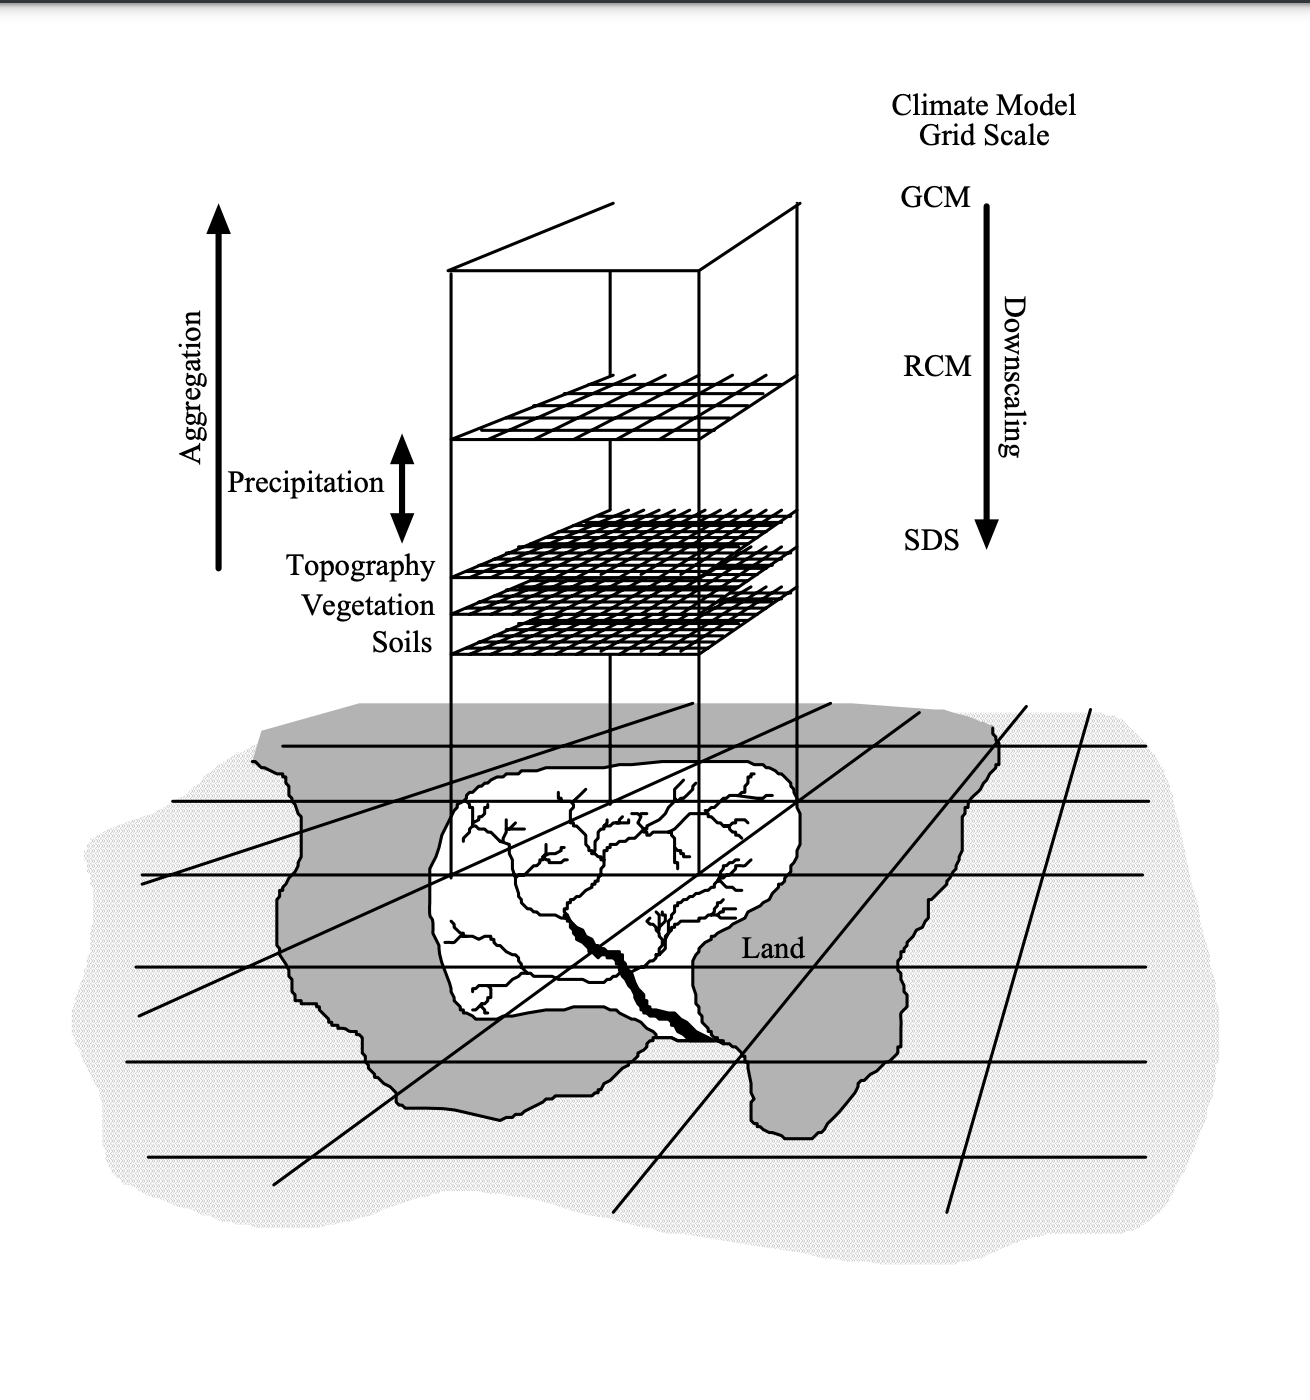
\includegraphics[width=0.8\linewidth]{./work/06-lowflow/figures/Figure_4} 

}

\caption{Schematic illustration of SDSM}(\#fig:fig4\_gamze)
\end{figure}

\emph{Source: SDSM Project Team, 2024}

This issue can be addressed through a technique known as downscaling. The statistical downscaling model (SDSM) developed by Wilby et al.~(2002) serves as a decision support tool for assessing local climate change impacts. SDSM can be best described as a hybrid of stochastic weather generator and regression-based methods. It employs a robust statistical downscaling technique that combines a weather generator and multiple linear regression. SDSM uses large-scale daily circulation patterns and atmospheric moisture variables (\(j = 1, 2, \ldots, n\)) to linearly condition local-scale weather generator parameters (e.g., precipitation occurrence and intensity) at individual sites. It generates local weather scenarios by combining weather generator outputs with future climate scenarios projected by GCMs.

The diagram \ref{fig:fig5} illustrates the general approach of SDSM, showing how it integrates both NCEP predictors and GCM predictors through a downscale predictand process. First, the NCEP predictors feed into a weather generator. Then, the simulated historical data coming from weather generator is assessed using the Nash-Sutcliffe efficiency (NSE) between the simulated and observed meteorological variables of interest. With the input of the GCMs large-scale predictors and outputs of the weather generator, future values for the meteorological variable of interest are generated by the scenario generator. Both the weather generator and the scenario generator contribute to the model output, which represents the localized weather patterns and events based on projected climate changes.

\begin{figure}

{\centering 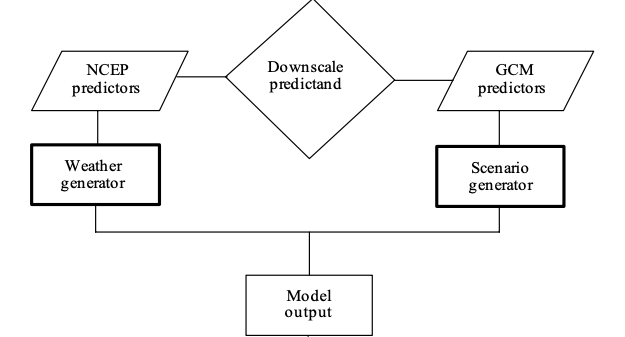
\includegraphics[width=0.8\linewidth]{./work/06-lowflow/figures/Figure_5} 

}

\caption{SDSM Climate Scenario Generation}(\#fig:fig5\_gamze)
\end{figure}

\emph{Source: SDSM Project Team, 2024}

It has been widely used in climate change research (Wilby and Dawson, 2013) and is comprehensively described in Wilby et al.~(2002) and Wilby and Dawson (2007).

Theoretically, the downscaling process with SDSM can be either unconditional or conditional on an event. For the unconditional process, a direct multiple linear regression equation is constructed between the unconditional predictand \(y_{i}^{UC}\) and the chosen normalized large-scale predictors \(\hat{u}_{i}^{j}\) on day \(i\) (\citet{Wilby2003}, \citet{Wetterhall2006}):

\[
y_{i}^{U C}=\gamma_{0}+\sum_{j=1}^{l} \gamma_{j} \hat{u}_{i}^{j}+\varepsilon \tag{28}
\]

where \(\gamma_{j}\) are the estimated regression coefficients determined by the least squares method, \(l\) is the number of selected predictors, and \(\varepsilon\) is a normally distributed stochastic error term.

For the conditional process, the conditional probability of predictand occurrence \(\omega_{i}\) on day \(i\) is directly represented as a multiple linear regression equation of \(\hat{u}_{i}^{j}\):

\[
\omega_{i}=\eta_{0}+\sum_{j=1}^{l} \eta_{j} \hat{u}_{i}^{j}\tag{29}
\]

where \(\eta_{j}\) are the estimated regression coefficients. If \(\omega_{i} \leqslant r_{i}\), where \(r_{i}\) is a uniformly distributed random number (\(0 \leqslant r_{i} \leqslant 1\)), the conditional predictand \(y_{i}^{c}\) occurs with an amount of:

\[
y_{i}^{C}=F^{-1}\left[\Phi\left(Z_{i}\right)\right] \tag{30}
\]

where \(F\) is the empirical distribution function of \(y_{i}^{c}\), and \(\Phi\) is the normal cumulative distribution function. \(Z_{i}\) is the \(z\)-score for day \(i\), expressed as \(Z_{i}=\lambda_{0}+\sum_{j=1}^{l} \lambda_{j} \hat{u}{i}^{j}+\varepsilon\), where \(\lambda{j}\) are the estimated regression coefficients.

The simulation results were assessed by the Nash-Sutcliffe efficiency (NSE) between the simulated and observed Temp and Prep. NSE is calculated as (\citet{Nash1970}):

\[
N S E=1-\frac{\sum_{i=1}^{\tau}\left(Y_{i}^{\text {obs }}-Y_{i}^{\text {sim }}\right)^{2}}{\sum_{i=1}^{\tau}\left(Y_{i}^{\text {obs }}-Y^{\text {mean }}\right)^{2}}\tag{31}
\]

where \(Y_{i}^{\text {obs }}\) are the observed meteorological variables, \(Y_{i}^{\text {sim }}\) are the simulated values corresponding to \(Y_{i}^{o b s}, Y^{\text {mean }}\) is the mean value of \(Y_{i}^{\text {obs }}\). NSE ranges from \(-\infty\) to 1, with \(N S E=1\) being the perfect simulation.

Typically, the predictand-predictor relationship in the SDSM, represented by the calibrated multiple linear regression equation, is assumed to be transferable to future projection periods (\citet{Wilby2002}, \citet{Wilby2007}, \citet{Wilby2013}, \citet{Wetterhall2006}, \citet{Mullan2012}). Using the large-scale predictors from GCMs as input, future scenarios of the meteorological variables of interest can then be derived, providing localized weather patterns and events based on projected climate changes.

\textbf{Statistical Downscaling Model (SDSM) in Du et al.~(2015)}

Du et al.~(2015) employed the Statistical Down Scaling Model developed by Wilby et al.~(2002) as a decision support tool for assessing local climate change impacts.

\textbf{Key Features of SDSM}:

- \textbf{Unconditional Process} is used for the simulation of temperature.

- \textbf{Conditional Process} is used for the simulation of precipitation.

\textbf{Downscaling Procedure}:

\begin{itemize}
\item
  \textbf{Selection of Predictors}: Mean sea level pressure, 500 hPa geopotential height, 500 hPa eastward wind, 850 hPa air temperature, and near-surface air temperature were selected for downscaling daily average temperature. For daily total precipitation, 850 hPa specific humidity was included.
\item
  \textbf{Model Calibration}: SDSM was calibrated using National Centers for Environmental Prediction (NCEP) reanalysis data to establish the relationship between predictands (daily average temperature and daily total precipitation) and large-scale predictors.
\item
  \textbf{Simulation}: Daily average temperature and daily total precipitation for the period 1954--2009 were simulated using SDSM driven by NCEP reanalysis predictors. The Nash-Sutcliffe Efficiency (NSE) between the simulated and observed data was used to assess model performance.
\item
  \textbf{Future Projections}: The calibrated SDSM model was used to generate future scenarios of temperature and precipitation for 2010-2099 based on predictors from multiple GCMs under the RCP8.5 scenario.
\end{itemize}

\textbf{Results}:

\begin{itemize}
\tightlist
\item
  The simulated data for 1954-2009 showed adequate agreement with observed data, particularly for temperature. - Future projections indicated strong increasing trends in temperature for both Huaxian and Xianyang stations, while precipitation remained relatively stable for Huaxian.
\item
  The use of SDSM allowed Du et al.~(2015) to effectively incorporate climate change projections into their nonstationary frequency analysis of low-flow events, providing valuable insights for water resource management under changing climatic conditions.
\item
  It should be noted that there are uncertainties in the downscaled future scenarios of meteorological variables used in this study. These uncertainties could be partially mitigated by exploring additional downscaling methods and different General Circulation Models (GCMs).
\end{itemize}

\section{Conclusion}\label{conclusion-3}

In this chapter, we delved into the complex nature of low-flow events, emphasizing their prediction and analysis through advanced hydrological frequency models. Low-flow events, characterized by significantly reduced streamflow and water availability, pose serious challenges to water resource management, especially under changing climatic conditions. Our exploration highlighted the critical role of return periods and risk assessments in understanding and mitigating the impacts of these events.

Traditional hydrological models, which assume stationarity, rely on historical data to predict future occurrences of low-flow events. However, this assumption is increasingly challenged by the evident impacts of climate change and human activities, which alter hydrological processes over time. Nonstationary models, which account for these dynamic factors, provide a more accurate and realistic approach to predicting low-flow events.

One of the key advancements in nonstationary hydrological analysis is the incorporation of time-varying parameters and meteorological covariates. By integrating these factors, nonstationary models can better capture the evolving nature of low-flow events. Meteorological covariates, such as temperature and precipitation, have been shown to significantly enhance the accuracy of low-flow predictions by linking hydrological responses to climatic conditions. This approach allows for a more nuanced understanding of how climate change influences hydrological extremes.

The use of copulas in bivariate analysis further enriches our understanding of low-flow events by modeling the dependencies between multiple hydrological variables. Time-varying copulas, which allow the dependence structure between variables to evolve over time, offer a sophisticated method for analyzing the joint behavior of hydrological extremes. This is particularly useful in assessing the risk and return periods of compound extreme events, where multiple variables interact to influence the occurrence and severity of low-flow conditions.

Reservoir indices, which account for the impact of reservoir operations on flow regimes, also play a crucial role in low-flow predictions. These indices provide a more comprehensive view of how human interventions, such as water withdrawals and reservoir management, affect streamflow patterns. By integrating reservoir indices into nonstationary models, we can better predict low-flow events in regulated river systems.

The hybrid dynamical--statistical approach, exemplified by the Statistical Downscaling Model (SDSM), represents another significant advancement in hydrological modeling. This approach combines the strengths of both dynamical and statistical methods, using climate model outputs to predict future hydrological conditions at a local scale. SDSM effectively bridges the gap between large-scale climate projections and localized hydrological impacts, providing valuable insights for water resource management under future climate scenarios.

The integration of nonstationary models, meteorological covariates, and advanced statistical methods offers a more robust framework for understanding and predicting low-flow events. These approaches provide a more accurate and comprehensive view of hydrological extremes, enabling better preparation and mitigation strategies in water resource management.

Looking forward, the ongoing development and refinement of nonstationary models are crucial for enhancing our ability to predict and manage low-flow events. As future research addresses the expansion of explanatory variables, improvements in model accuracy, and the integration of more comprehensive datasets, these efforts will enable the creation of more resilient and adaptive water management strategies, effectively tackling the challenges posed by climate change and other dynamic factors.

\chapter{Statistical streamflow modelling}\label{sm}

\emph{Author: Lennart Marx}

\emph{Supervisor: Henri Funk}

\emph{Degree: Master}

\section{Abstract}\label{abstract-4}

This study evaluates and compares the performance of Long Short-Term Memory (LSTM) networks and Temporal Fusion Transformers (TFT) in forecasting streamflows for up to seven day ahead forecasts, using historical streamflow data alongside precipitation and temperature as covariates. Freely available data published by the bavarian hydrological authority from the Regen river in Bavaria, Germany, was used in conjunction with meteorological data from the ERA5 reanalysis dataset. River basins are defined via the HydroRIVERS and HydroBASINS dataset to obtain the area over which precipitation is aggregated. Results indicate that while both models face challenges in predicting extreme values, TFT maintains more consistent accuracy over longer forecast horizons while pure LSTM model's predictions decline sharply in performance with increasing lead times.

\section{Introduction}\label{introduction-5}

Streamflow forecasting plays a crucial role in water resource management, particularly in flood prediction. As climate change intensifies extreme weather events and alters precipitation patterns, accurate streamflow forecasts have become increasingly important for mitigating flood risks by providing information about the timing and magnitude of potential flood events.This knowledge enables authorities to implement timely flood control measures, operate reservoirs effectively, and issue early warnings to vulnerable communities. As flooding remains one of the most common and destructive natural disasters, especially in developing countries, improved forecasting capabilities can significantly reduce the human and economic toll of these events. (\citet{nearing2024})

Hydropower is the dominant source of renewable energy, accounting for 16\% of the world's electricity output and 62\% of renewable electricity generation (\citet{lee2022}). Precise streamflow predictions can be beneficial in optimizing reservoir operations. \citet{lee2022} show that this is the case for 94\% of all analyzed dams dependent on forecasting ability and reservoir characteristics.

A streamflow refers to the flow of water in rivers, streams or other water bodies, originating from precipitation, melting snow, and groundwater discharge. It is typically measured in cubic meters per second (m³/s).

In recent years, machine learning techniques have emerged as powerful tools for forecasting in various domains, including hydrology. Traditional hydrological models often rely on extensive datasets and intricate physical parameters, which can be challenging to obtain and process. In contrast, machine learning models such as Long Short-Term Memory (LSTM) networks offer an alternative approach by learning patterns directly from historical data.

This study aims to evaluate and compare the performance of LSTM and TFT models in forecasting streamflows up to seven days ahead. By incorporating precipitation and temperature as future known covariates alongside historical streamflow data, this work seeks to determine the effectiveness of these models in predicting streamflows.

\section{Data}\label{data-2}

\subsection{Preperation}\label{preperation}

The streamflow data is gathered from the bavarian hydrology authority (GKD). They provide freely accessible data on most water bodies in Bavaria \citet{gkd2024}. Focusing on rivers of medium size where the entire length of the river is located inside of the state of Bavaria, the river Regen positioned north/east of the city of Regensburg was chosen as a bases for this study. The GKD has data on 21 streamflow gauging stations located at the Regen or any of its tributary rivers. For the Regen river, data between 2014 and 2024 is available with daily measurements on the streamflows including the coordinates of the the gauging station. This study focused on the 15207507 Marienthal gauging station that was located closest to the final outflow towards the Danube river within the city of Regensburg. Utilizing the HydroRIVERS dataset, which contains the shapes of rivers all over the world, it was possible the acquire the shape of the Regen along with its geolocation as shown in figure \ref{fig:regen-shape} \citet{lehner2008}.

\begin{figure}

{\centering \includegraphics[width=0.7\linewidth]{work/07-hydroLSTM/images/regen_stations} 

}

\caption{Streamflow gauging stations that provide there measurements at the GKD along the Regen river (adapted from @OpenStreetMap2017)}\label{fig:regen-shape}
\end{figure}

A catchment also known as a drainage basin or watershed, is an area of land where all precipitation collects and drains off into a common outlet, such as a river, bay, or other body of water. The boundaries of a catchment are defined by the highest points of land around the drainage area, often referred to as the drainage divide. These catchment areas will later be used to determine the variables for precipitation that are used to forecast the streamflows of the river. Taking advantage of the HydroBASINS dataset, that contains the shapes of basins all over the world in different resolutions \citet{lehner2008}. With the software QGIS a geoinformation system (GIS) all basins were chosen that completely contain the river Regen shape, which led to the 19 defined catchments that can be seen figure \ref{fig:regen-catch}.

\begin{figure}

{\centering \includegraphics[width=0.7\linewidth]{work/07-hydroLSTM/images/river_catch} 

}

\caption{Catchments defined for the Regen river based on the HydroBASINS shapefile dataset (adapted from @OpenStreetMap2017)}\label{fig:regen-catch}
\end{figure}

The ERA5 reanalysis dataset, contains a plethora of meteorological data in a rasterized form. Each data cell contains information of when it occured, where it occured in the form of longitude and latitude coordinates as well as the information on a meteorological variables \citet{hersbach2023}. As proposed in \citet{sabzipour2023}, for this study the variables 2 meter temperature and total precipitation were selected around the area of the Regen and for the past 10 years.

\subsection{Preprocessing}\label{preprocessing}

The measuring station 15207507 contained 1 missing value which was imputed by linear interpolation. As suggested in \citet{sabzipour2023} non centered moving average smoothing with a window size of 3 was applied to the streamflow data as can be seen in figure \ref{fig:marien-stream}.

\begin{figure}

{\centering 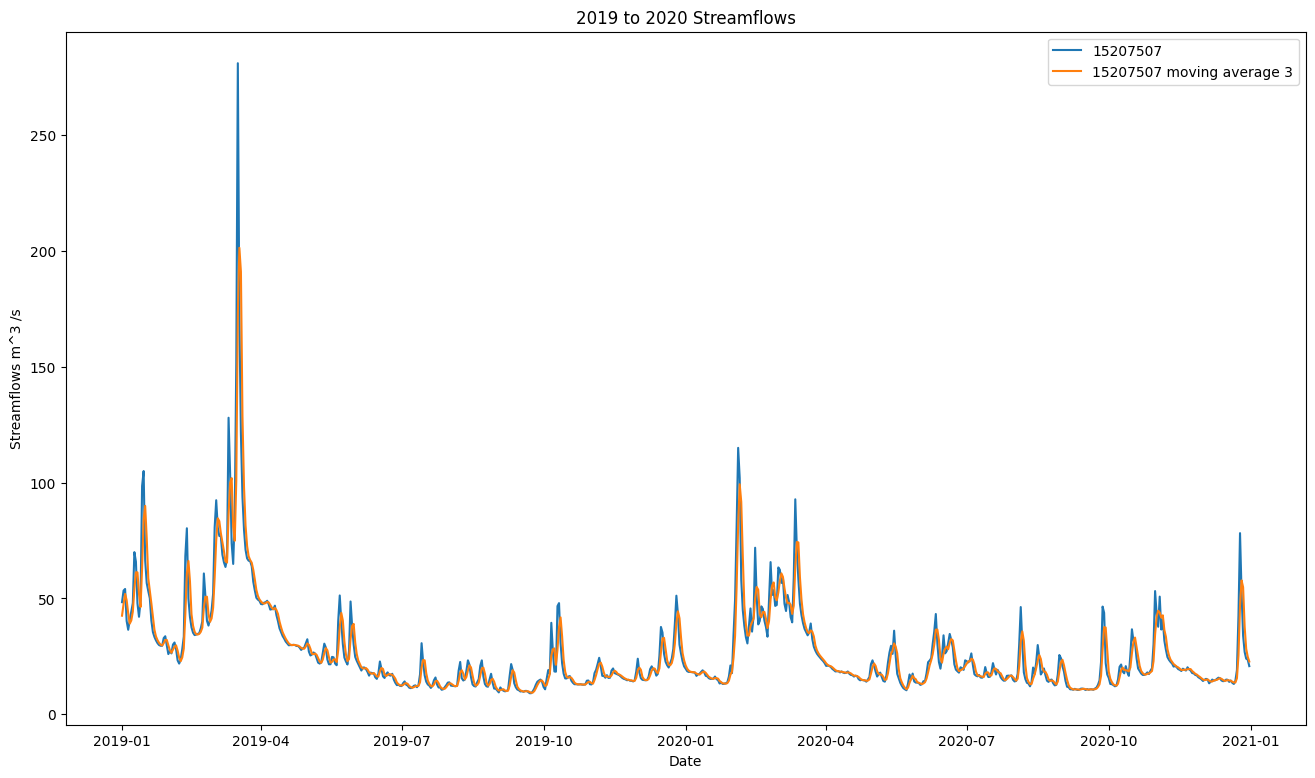
\includegraphics[width=0.8\linewidth]{work/07-hydroLSTM/images/Moving_Average} 

}

\caption{streamflows of the 15207507 Marienthal gauging stations before (blue) and after (orange) applying moving average smoothing}\label{fig:marien-stream}
\end{figure}

To combine the rasterized meteorological data from ERA5 with the streamflows of the Regen, it is necessary to only take precipitation into account that occurs within the defined catchments. To achieve this, a weighted average is calculated, where the weights are determined by the area size of the intersection between the raster cell of the meteorological data and the catchment. This can be seen in a schematic visualization in figure \ref{fig:spatial-avg}.

\begin{figure}

{\centering 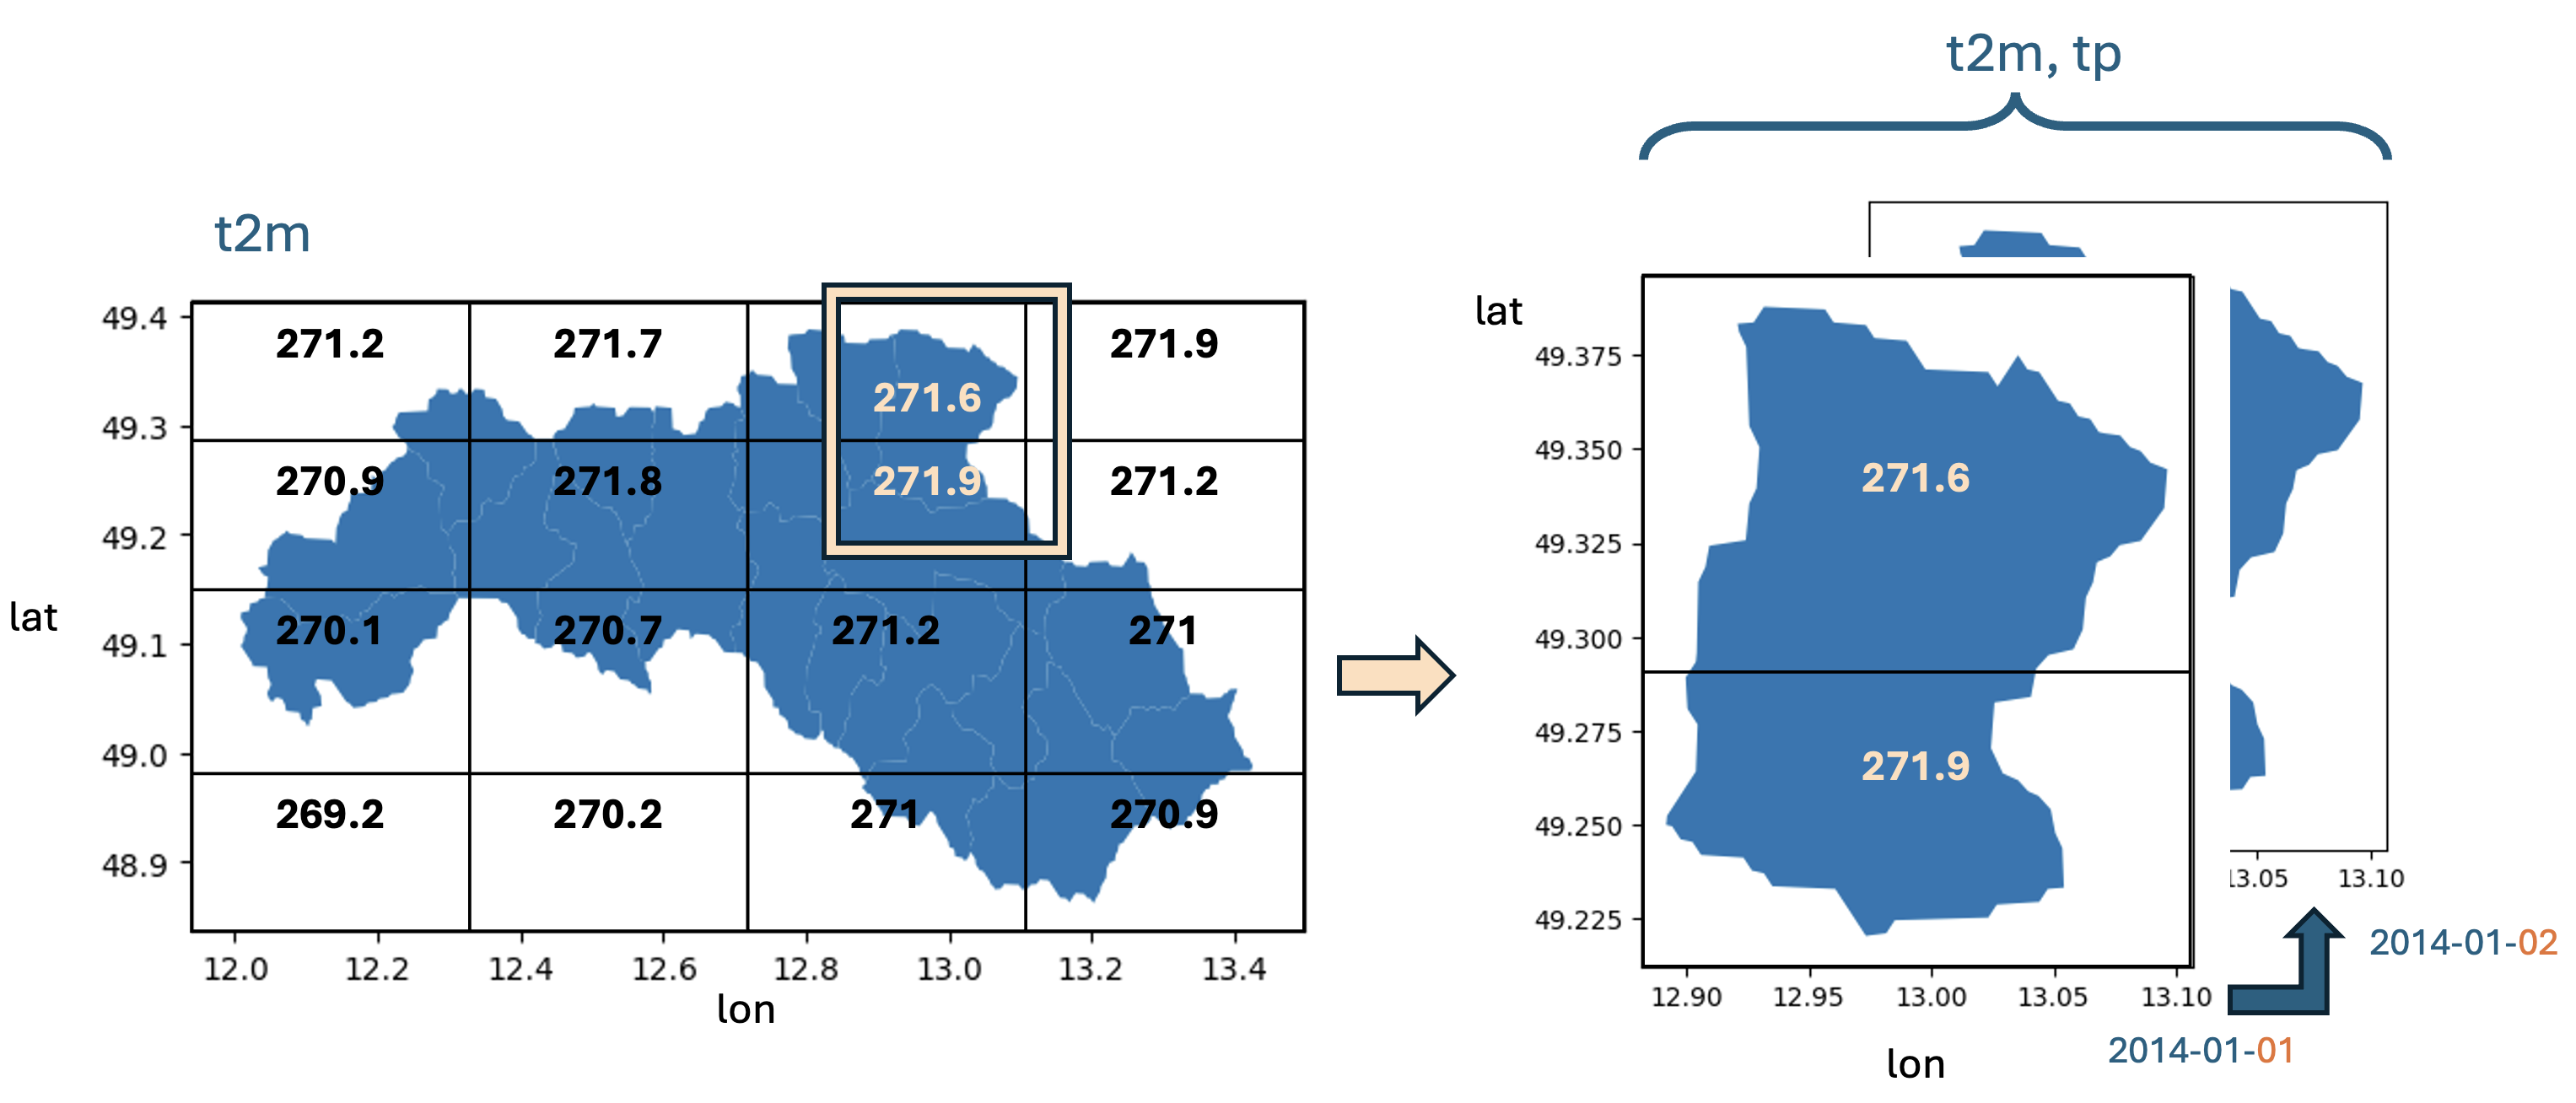
\includegraphics[width=0.8\linewidth]{work/07-hydroLSTM/images/spatial_averaging} 

}

\caption{schematic visualization of the spatial averaging performed for temperature and total precipitation during data preprocessing}\label{fig:spatial-avg}
\end{figure}

\[ tp(\text{catch}_i) = \frac{1}{A(\text{catch}_i)} \sum_{cell_j \in \text{ERA5 raster}} \left( tp(\text{cell}_j) \cdot A(\text{catch}_i \cap \text{cell}_j) \right) \tag{1} \]

A : area\\
catch : catchment\\
cell : one cell in the raster data set of ERA5\\
tp : total precipitation

Since the catchments are geospatially very close to each other, the different catchments are highly correlated to each other and therefore provide little variance (see Figure \ref{fig:tp-corr}). To reduce the feature space for both variables temperature and precipitation, the mean is taken over all catchments. Finally to reduce the noise in the features a moving average of window size 3 was applied.

\begin{figure}

{\centering 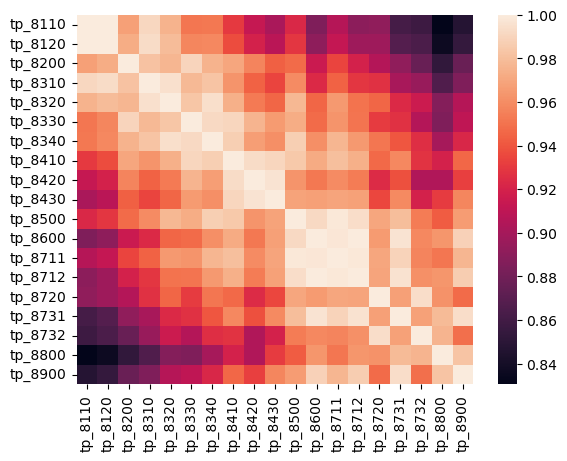
\includegraphics[width=0.7\linewidth]{work/07-hydroLSTM/images/tp_correlation_table} 

}

\caption{correlation table for total precipitation over all catchments}\label{fig:tp-corr}
\end{figure}

\section{Models}\label{models}

\subsection{LSTM}\label{lstm}

The Long Short-Term Memory (LSTM) cell (figure \ref{fig:lstm}) is a type of recurrent neural network (RNN) architecture designed to model temporal sequences and their long-range dependencies more accurately than traditional RNNs. LSTMs were introduced by Sepp Hochreiter and Jürgen Schmidhuber in 1997 to address the issue of vanishing and exploding gradients encountered in traditional RNNs \citet{hochreiter1997}.

\begin{figure}

{\centering 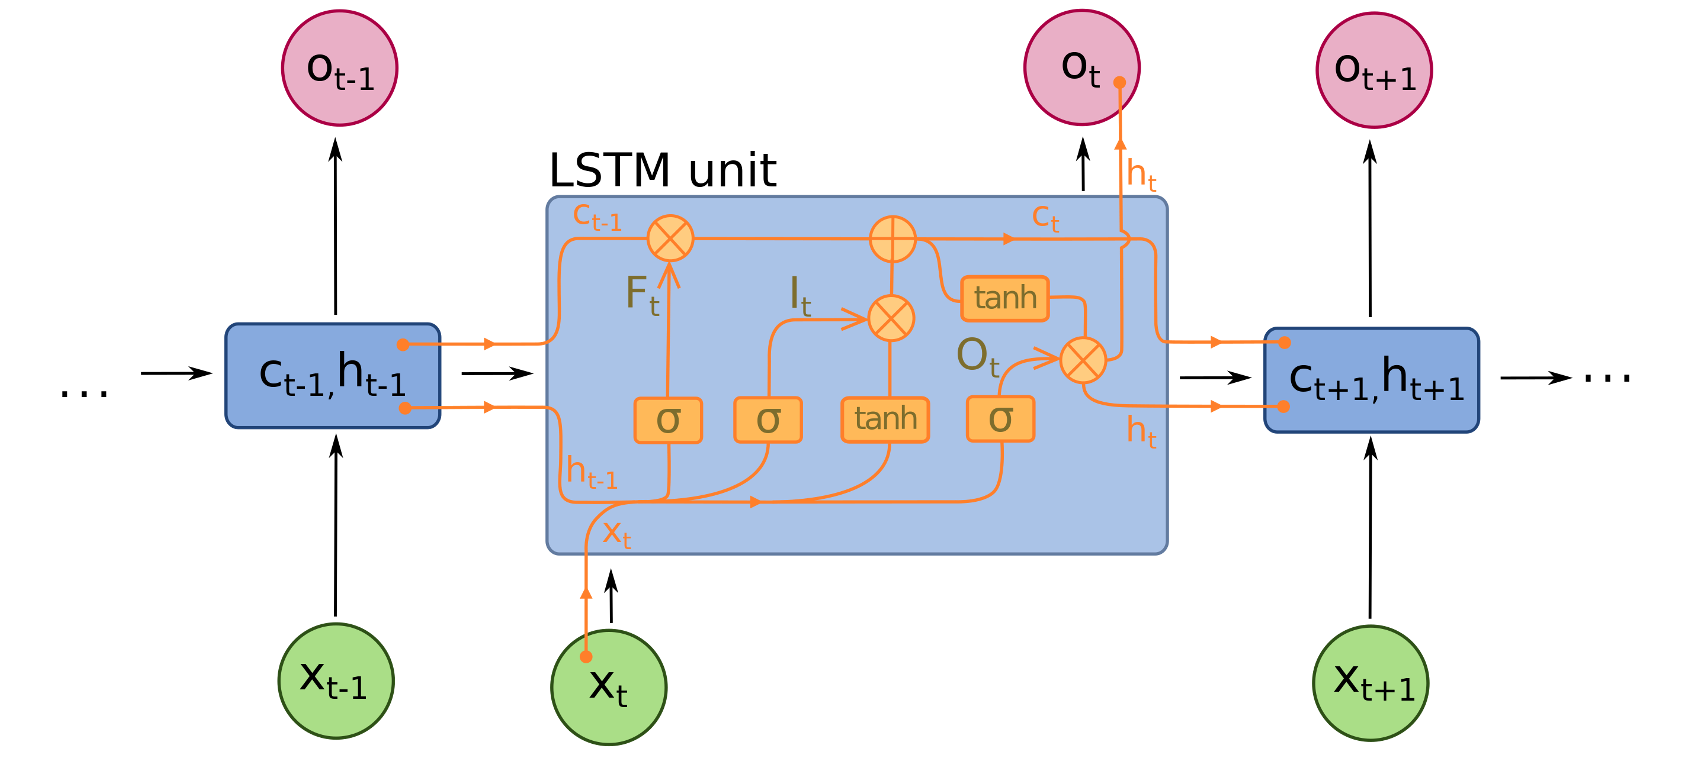
\includegraphics[width=0.7\linewidth]{work/07-hydroLSTM/images/LSTM} 

}

\caption{visualization of a LSTM cell at time step t (image adapted from @chevalier2023)}\label{fig:lstm}
\end{figure}

\begin{enumerate}
\def\labelenumi{\arabic{enumi}.}
\tightlist
\item
  \textbf{Cell State (}\(C_t\)): The internal memory of the cell, which can carry information across many time steps.
\item
  \textbf{Hidden State (}\(h_t\)): The output of the LSTM cell at a given time step, also serving as the input to the next cell.
\item
  \textbf{Input Gate (}\(i_t\)): Controls how much of the new information from the current input is used to update the cell state.
\item
  \textbf{Forget Gate (}\(f_t\)): Decides how much of the past cell state should be forgotten.
\item
  \textbf{Output Gate (}\(o_t\)): Determines the output of the LSTM cell based on the cell state.
\end{enumerate}

LSTMs are particularly well-suited for tasks that involve sequential data and temporal dependencies, such as:

\begin{enumerate}
\def\labelenumi{\arabic{enumi}.}
\tightlist
\item
  \textbf{Natural Language Processing (NLP)}:

  \begin{itemize}
  \tightlist
  \item
    Language modeling
  \item
    Machine translation
  \item
    Speech recognition
  \end{itemize}
\item
  \textbf{Time Series Forecasting}:

  \begin{itemize}
  \tightlist
  \item
    Stock price prediction
  \item
    Weather forecasting
  \item
    Anomaly detection
  \end{itemize}
\end{enumerate}

Streamflow forecasting involves predicting the flow of water in rivers and streams over time, which is inherently a time-series problem with temporal dependencies influenced by various factors such as rainfall, snowmelt, and upstream water management. When used in an encoder decoder architecture LSTM-cells can also incorporate future known covariates such as weather forecasts. These specifications make LSTM-based architectures beneficial for modeling and forecasting streamflow data.

\subsection{Temporal Fusion Transformer}\label{temporal-fusion-transformer}

The Temporal Fusion Transformer (TFT) (figure \ref{fig:tft}) is a neural network architecture specifically designed for multi-horizon time series forecasting. It combines the strengths of both recurrent and attention-based models, offering an advanced approach to handling complex time series data. The TFT was introduced by Bryan Lim et al.~in 2019, aiming to provide interpretability and accuracy for forecasting tasks \citet{lim2021}.

\begin{figure}

{\centering 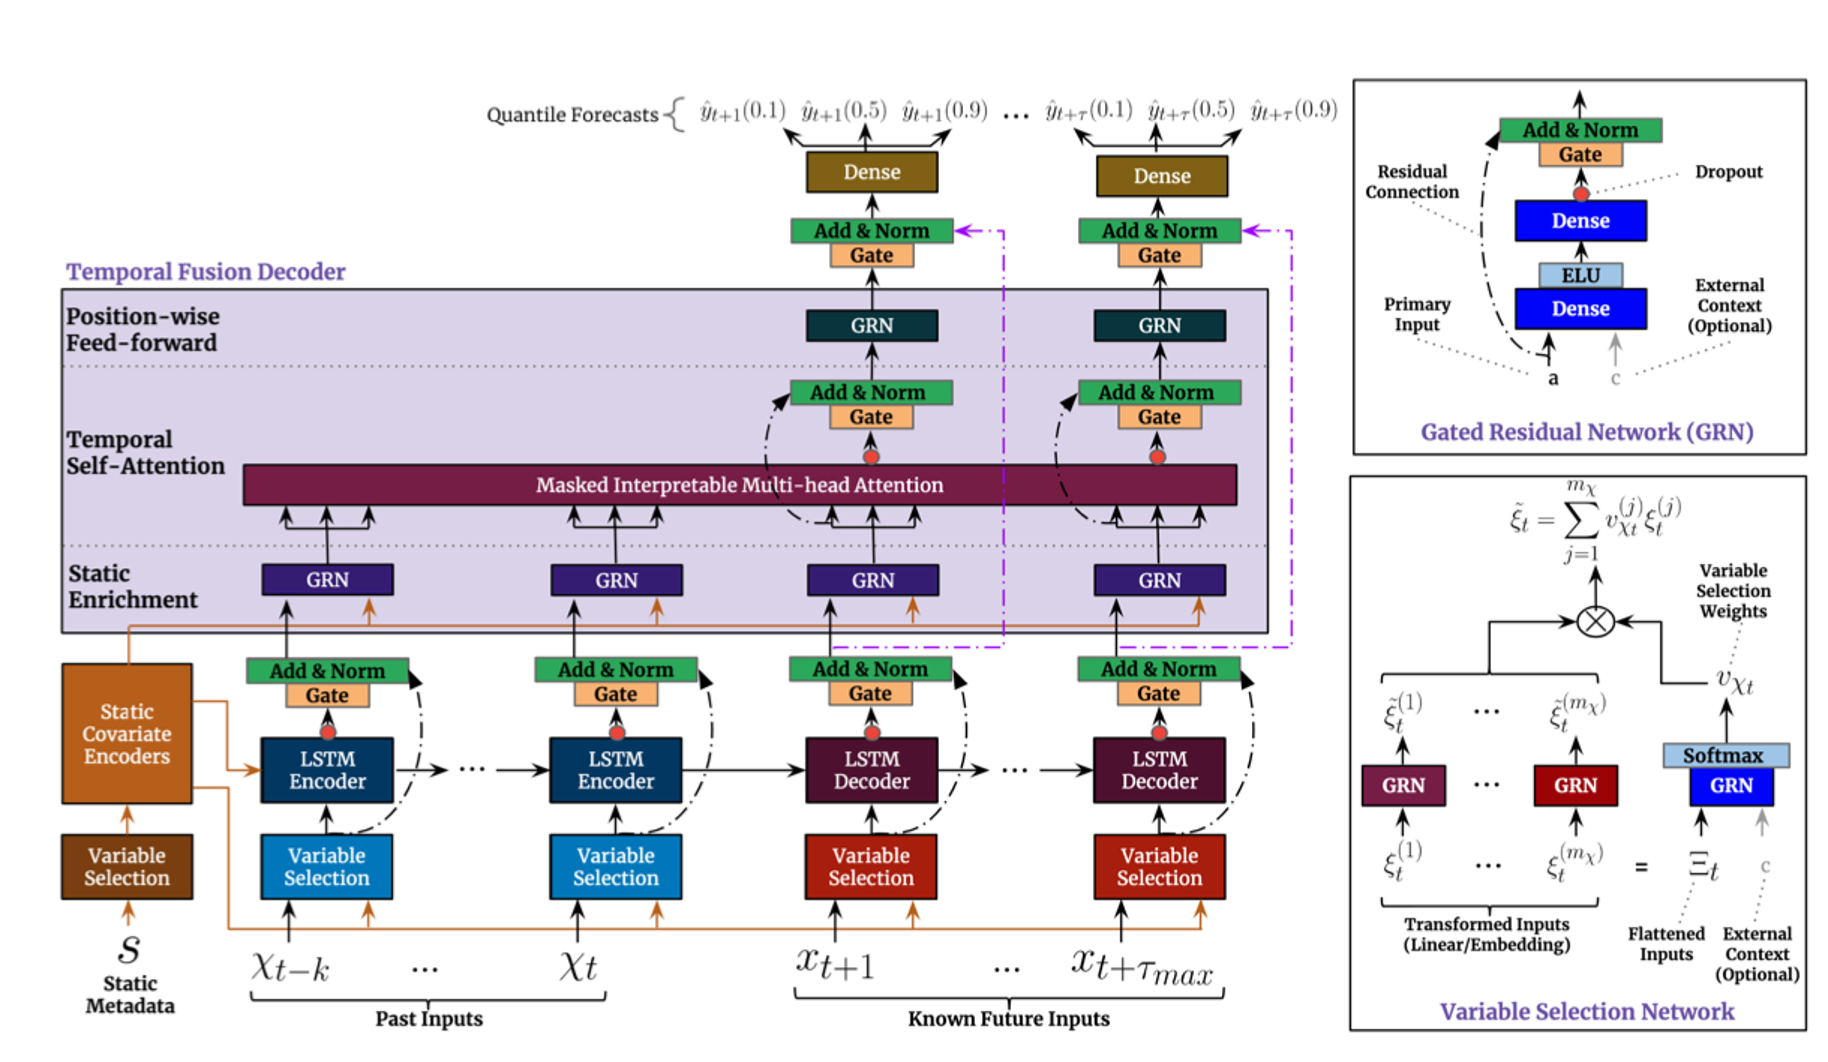
\includegraphics[width=0.8\linewidth]{work/07-hydroLSTM/images/TFT} 

}

\caption{model architecture for the Temporal Fusion Transformer (image from @lim2021}\label{fig:tft}
\end{figure}

A TFT consists of several key components:

\begin{enumerate}
\def\labelenumi{\arabic{enumi}.}
\tightlist
\item
  \textbf{Temporal Processing}:

  \begin{itemize}
  \tightlist
  \item
    \textbf{Local Processing with LSTMs}: LSTMs are used to process local temporal dependencies within the time series.
  \item
    \textbf{Multi-Head Attention}: An attention mechanism to capture long-range dependencies across different time steps.
  \end{itemize}
\item
  \textbf{Variable Selection}:

  \begin{itemize}
  \tightlist
  \item
    \textbf{Static Covariate Encoders}: Handle static features that do not change over time (e.g., location-specific data).
  \item
    \textbf{Temporal Covariate Encoders}: Manage time-varying features (e.g., weather data, past values of the time series).
  \end{itemize}
\item
  \textbf{Gating Mechanisms}:

  \begin{itemize}
  \tightlist
  \item
    \textbf{Gated Residual Network (GRN)}: Ensures that only relevant information is passed through layers, improving the network's efficiency and interpretability.
  \item
    \textbf{Variable Selection Networks}: Dynamically select relevant variables at each time step to enhance model performance and interpretability.
  \end{itemize}
\item
  \textbf{Multi-Horizon Forecasting}:

  \begin{itemize}
  \tightlist
  \item
    \textbf{Sequence-to-Sequence Framework}: Allows the TFT to generate forecasts for multiple future time steps simultaneously.
  \end{itemize}
\item
  \textbf{Interpretable Outputs}:

  \begin{itemize}
  \tightlist
  \item
    \textbf{Attention Weights}: Provide insights into which time steps and variables the model is focusing on, aiding interpretability.
  \end{itemize}
\end{enumerate}

The Temporal Fusion Transformer represents an advancement in time series forecasting, offering both high accuracy and interpretability. Its ability to capture complex dependencies, dynamically select relevant features, and provide insights into the decision-making process makes it a useful tool for streamflow forecasting.

\subsection{Kling Gupta Efficiency}\label{kling-gupta-efficiency}

The Kling-Gupta Efficiency (KGE) is a statistical metric used to evaluate the performance of hydrological models by comparing simulated data to observed data. Developed by Gupta et al.~in 2009, the KGE addresses limitations found in traditional metrics such as the Nash-Sutcliffe Efficiency (NSE). The KGE decomposes the evaluation of model performance into three distinct components, providing a more comprehensive assessment. These components are correlation, bias, and variability, which help in understanding different aspects of the model's accuracy.

The KGE is calculated using the following formula:

\[ \text{KGE} = 1 - \sqrt{(r - 1)^2 + (\alpha - 1)^2 + (\beta - 1)^2} \tag{2} \]

\begin{itemize}
\item
  \(r\) is the Pearson correlation coefficient between the simulated and observed values.
\item
  \(\alpha\) is the bias ratio, defined as the ratio of the mean of the simulated values to the mean of the observed values.
\item
  \(\beta\) is the standard deviation ratio, defined as the ratio of the standard deviation of the simulated values to the standard deviation of the observed values.
\end{itemize}

\section{Results}\label{results-1}

\subsection{Training Setup}\label{training-setup}

The 2 different model architectures were trained using the historical streamflows as well as temperature and precipitation as covariates. Using an input sequence length of 364 days and an output lead time of up to 7 days. Temperature and precipitation can be used as future known values when considering weather forecasts. For example when trying to predict one step ahead forecast for the streamflow in addition to the past 364 days of precipitation values one can consider the precipitation forecast for the next day to get the best predictions possible.

The LSTM Model is run in an encoder decoder architecture, were the past 364 days are the input for an LSTM cell which returns a hidden state and an output as the encoder step. During the decoder step, the encoder hidden state is fed into the decoder LSTM together with the future known inputs. The model predicts incrementally in the sense that for example to predict a 3 step ahead forecast it firsts predicts 1 and 2 step forecast and uses both forecasts to then predict the 3 step prediction. Both model architectures were used from the pytorch-forecasting library. The models were retrained for the different lead times. The used hyperparameters for both models are shown in Table \ref{tab:tab-hyperparams}.

The dataset is split into 70\% train set, 15\% validation set and 15\% test set respectivell.

\begin{table}

\caption{\label{tab:tab-hyperparams}Hyperparameter comparison between LSTM and TFT.}
\centering
\begin{tabular}[t]{l|l|l}
\hline
Hyperparameter & LSTM & TFT\\
\hline
Batch Size & 128 & 128\\
\hline
Epochs & 100 & 80\\
\hline
Hidden Size & 128 & 128\\
\hline
Attention Head Size & - & 2\\
\hline
Learning Rate & 0.001 & 0.003\\
\hline
Dropout & 0.2 & 0.1\\
\hline
Weight Decay & 0.001 & 1e-04\\
\hline
Gradient Clipping & 0.1 & 0.1\\
\hline
Loss Function & Mean Absolute Error & Mean Absolute Error\\
\hline
Optimizer & Adam & Adam\\
\hline
Reduce on Plateau Patience & 7 & 7\\
\hline
Time Varying Known Features & t2m, tp & t2m, tp\\
\hline
Time Varying Unknown Features & streamflow 15207507 & streamflow 15207507\\
\hline
\end{tabular}
\end{table}

\subsection{Results}\label{results-2}

The models evaluated on the holdout test set show good performance for lead times of 1 and 2 days especially considering since the training and validation loss that is used is the MAE and not the KGE. The performance declines sharply for the LSTM model across the lead times while the decline for the TFT is more gradual as can be seen in Table \ref{tab:tab-results}.

\begin{longtable}[]{@{}rll@{}}
\caption{\label{tab:tab-results}Performance comparison between TFT and LSTM models across different lead times on a holdout test set. Better performing model for each lead time in bold}\tabularnewline
\toprule\noalign{}
Lead.Time & TFT.KGE & LSTM.KGE \\
\midrule\noalign{}
\endfirsthead
\toprule\noalign{}
Lead.Time & TFT.KGE & LSTM.KGE \\
\midrule\noalign{}
\endhead
\bottomrule\noalign{}
\endlastfoot
1 & 0.8352 & \textbf{0.9696} \\
2 & 0.7103 & \textbf{0.8821} \\
3 & 0.6410 & \textbf{0.6716} \\
4 & \textbf{0.6096} & 0.4943 \\
5 & \textbf{0.5901} & 0.4302 \\
6 & \textbf{0.5778} & 0.3312 \\
7 & \textbf{0.5717} & 0.3185 \\
\end{longtable}

Forecasting the peaks of the streamflows is challenging and neither model performs particularly well on this task. Especially when considering that the peaks were already drastically reduced due to the moving average smoothing of the target variable. The model routinely undershoots the observed true streamflows here shown for a lead time of 5 days for the LSTM Model and the TFT Model in figure \ref{fig:lstm-pred} and in figure \ref{fig:tft-pred} respectively. This behavior can be observed for all lead times except 1 and 2 days where the performance is reasonable even in the peaks.

\begin{figure}

{\centering 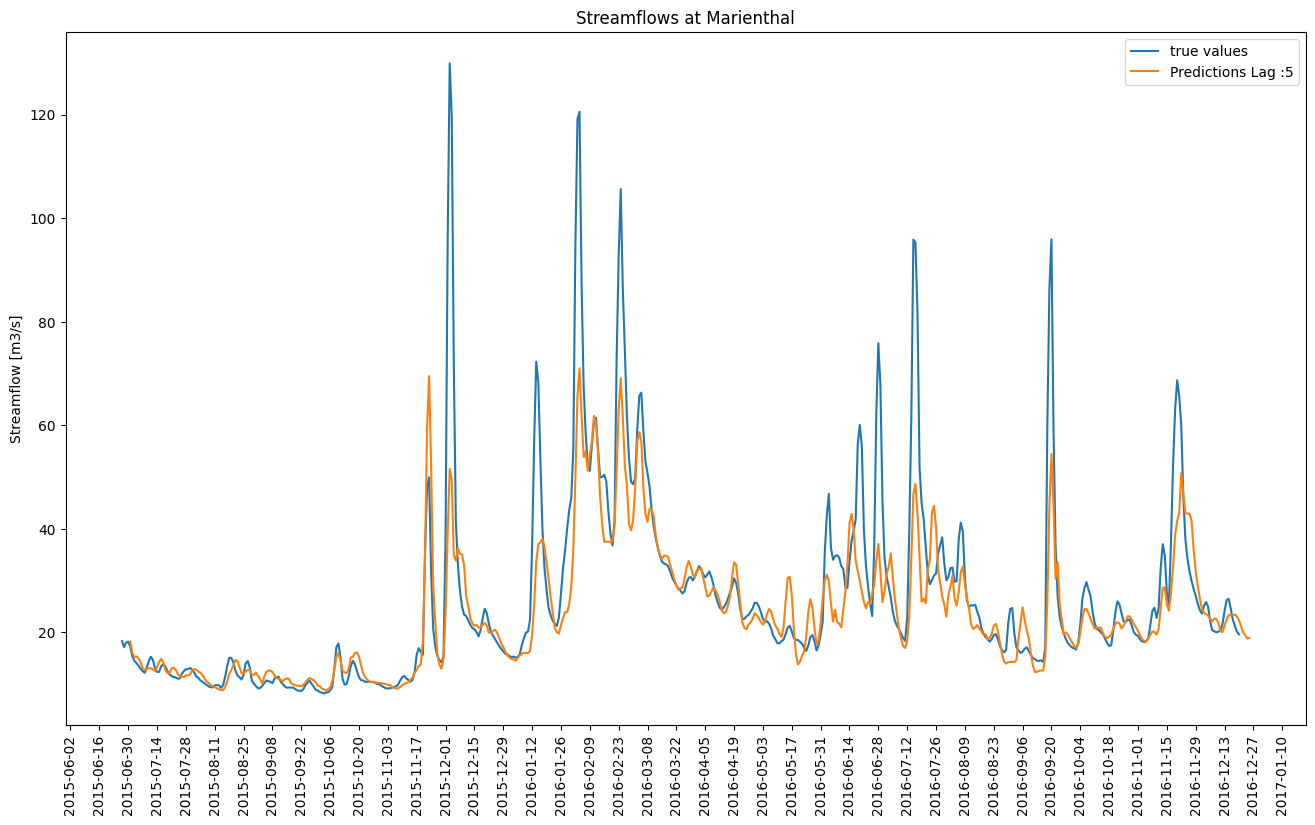
\includegraphics[width=0.8\linewidth]{work/07-hydroLSTM/images/lag5_lstm} 

}

\caption{LSTM predicted streamflows for a lead time of 5 days (orange) compared to the observed streamflows (blue)}\label{fig:lstm-pred}
\end{figure}

\begin{figure}

{\centering 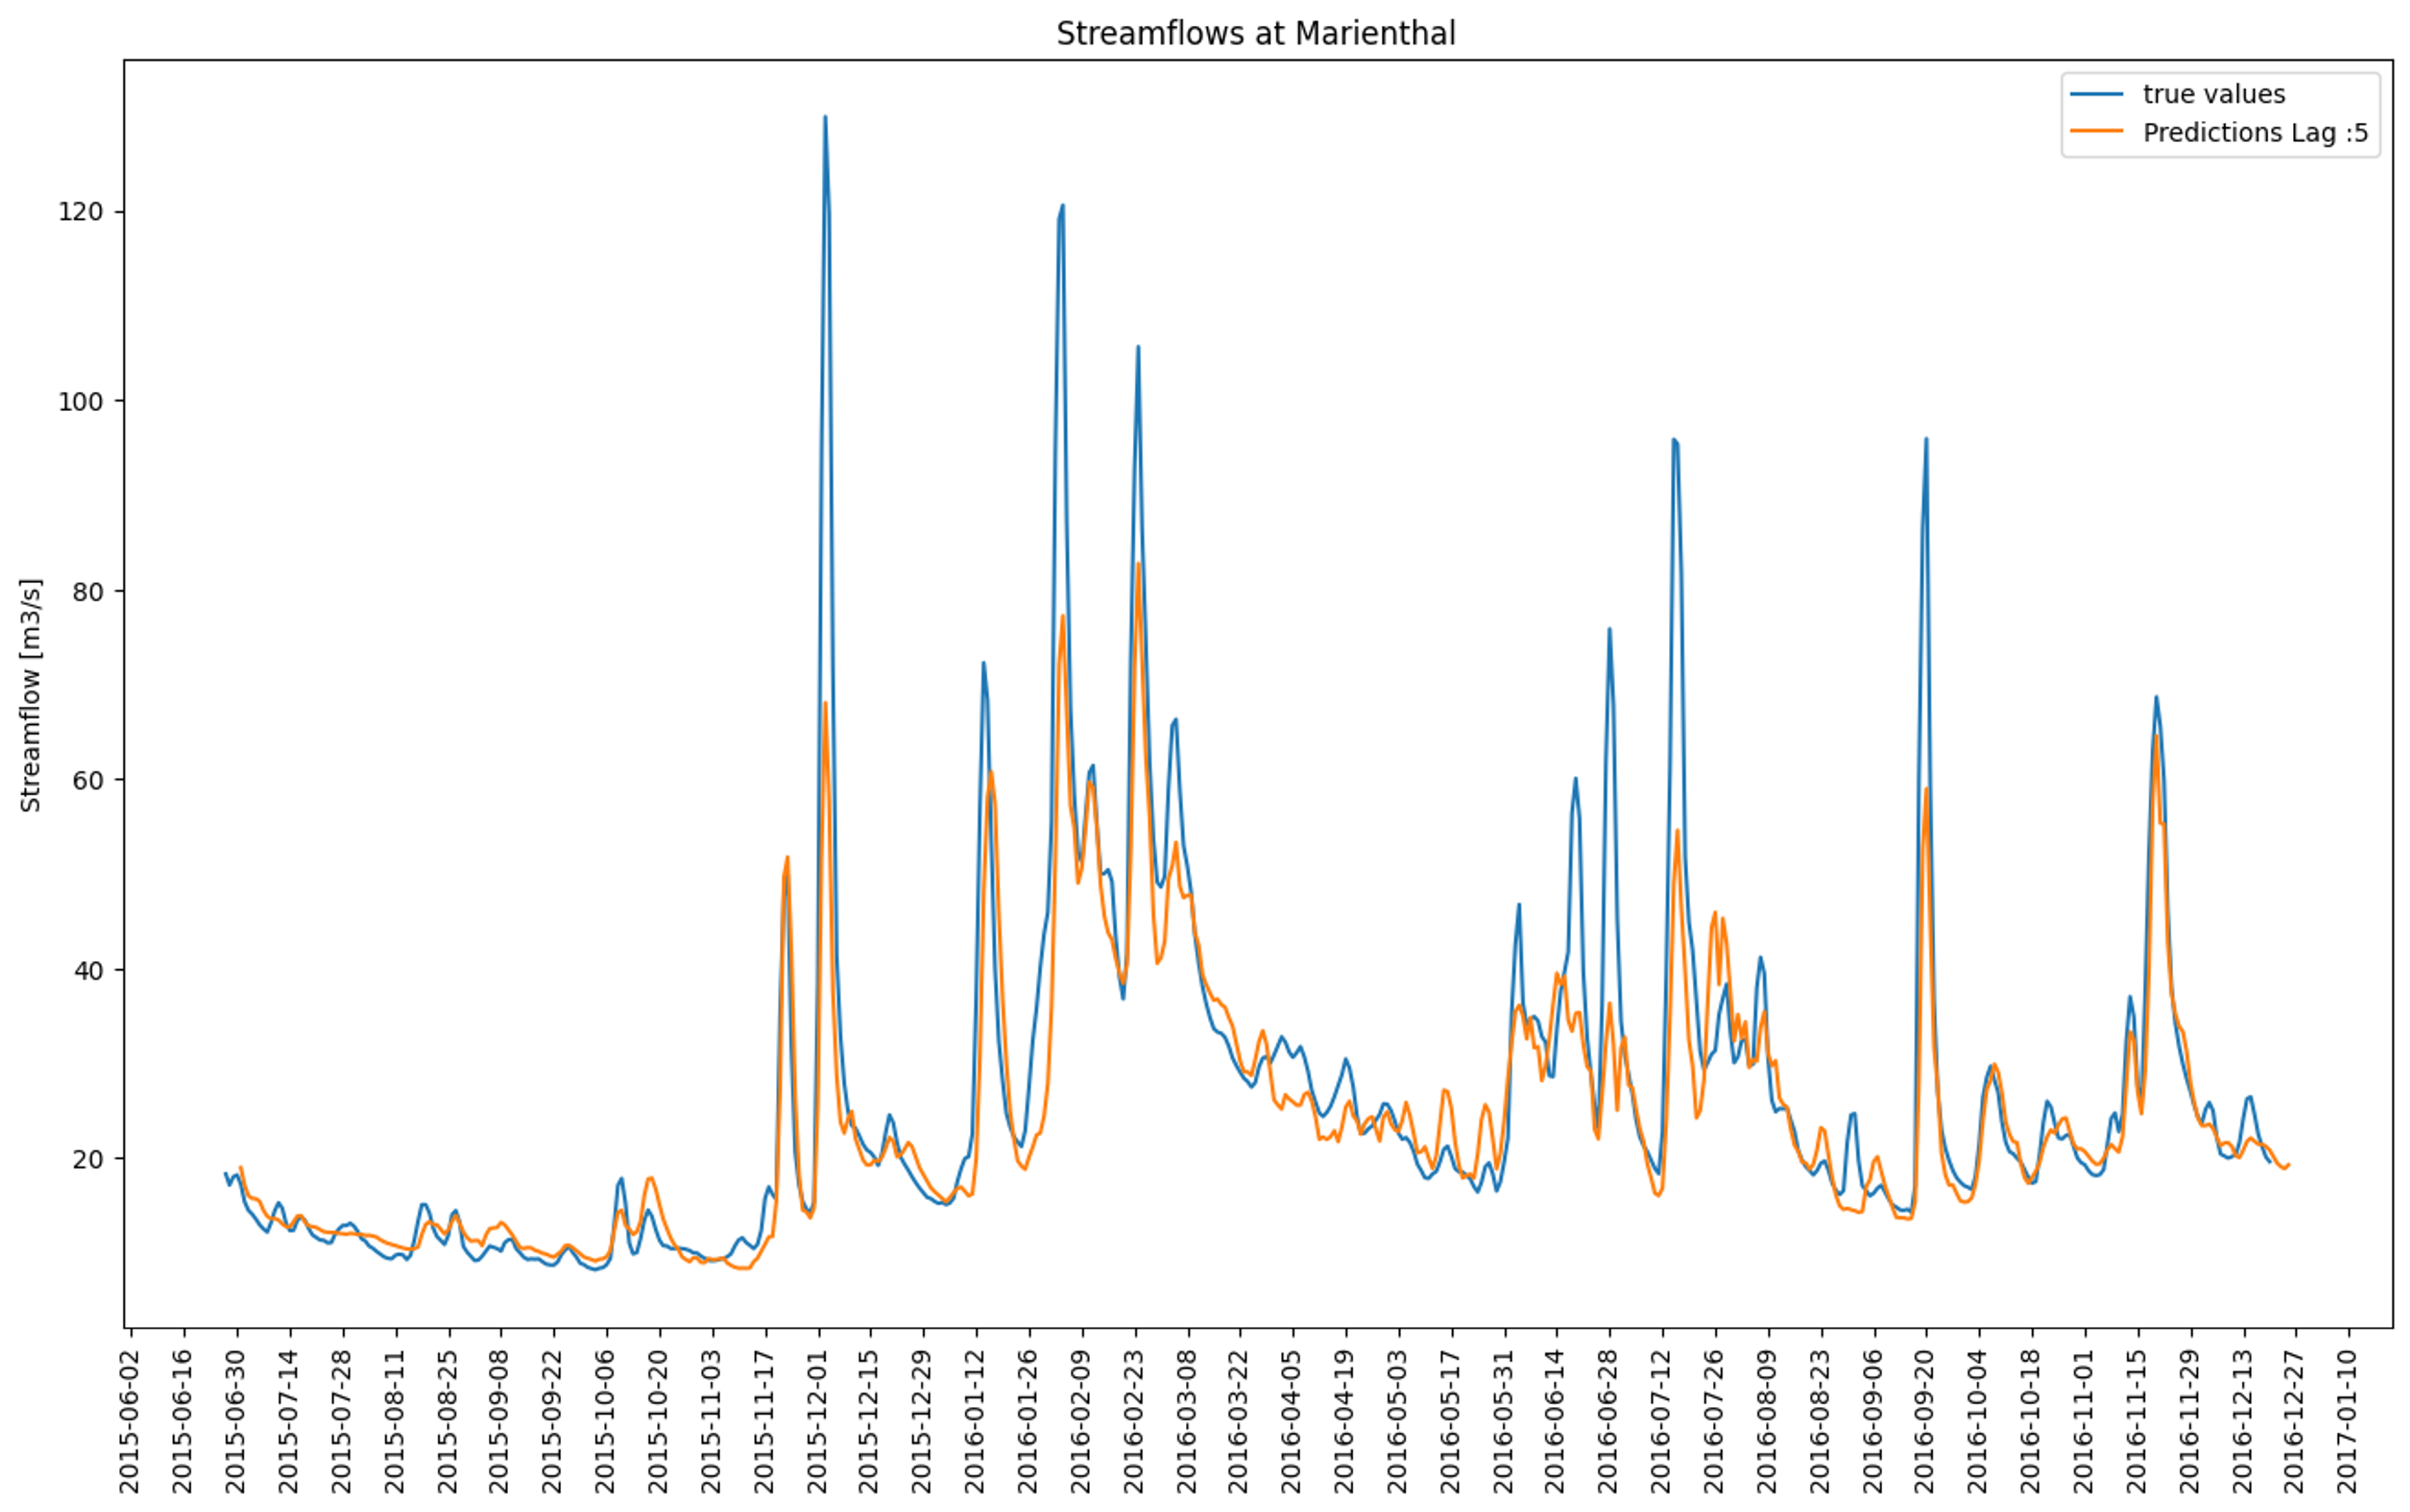
\includegraphics[width=0.8\linewidth]{work/07-hydroLSTM/images/lag5_tft} 

}

\caption{TFT predicted streamflows for a lead time of 5 days (orange) compared to the observed streamflows (blue)}\label{fig:tft-pred}
\end{figure}

\subsection{Feature Importance}\label{feature-importance}

For an inspection of feature dependence it is possible to make use of the inbuilt function that the pytorch-forecasting library provides. The models show very similar behavior for both used covariates. As can be seen in \ref{fig:tp-tft-imp} the TFT model observes a slightly stronger relationship between high total precipitation and large streamflows, but the plot for for both models has the expected shape, that high precipitation leads to high streamflows and vice versa.

In analyzing the relationship between t2m and streamflow, both graphs demonstrate a positive relationship. Specifically, the TFT dependence plot in Figure \ref{fig:t2m-tft-imp} shows an increase up to approximately 280 K, beyond which the effect plateaus. Similarly, the LSTM model depicted in Figure \ref{fig:t2m-lstm-imp} shows a more gradual increase, with the effect leveling off at higher mean temperatures of around 295 K.

\begin{figure}

{\centering 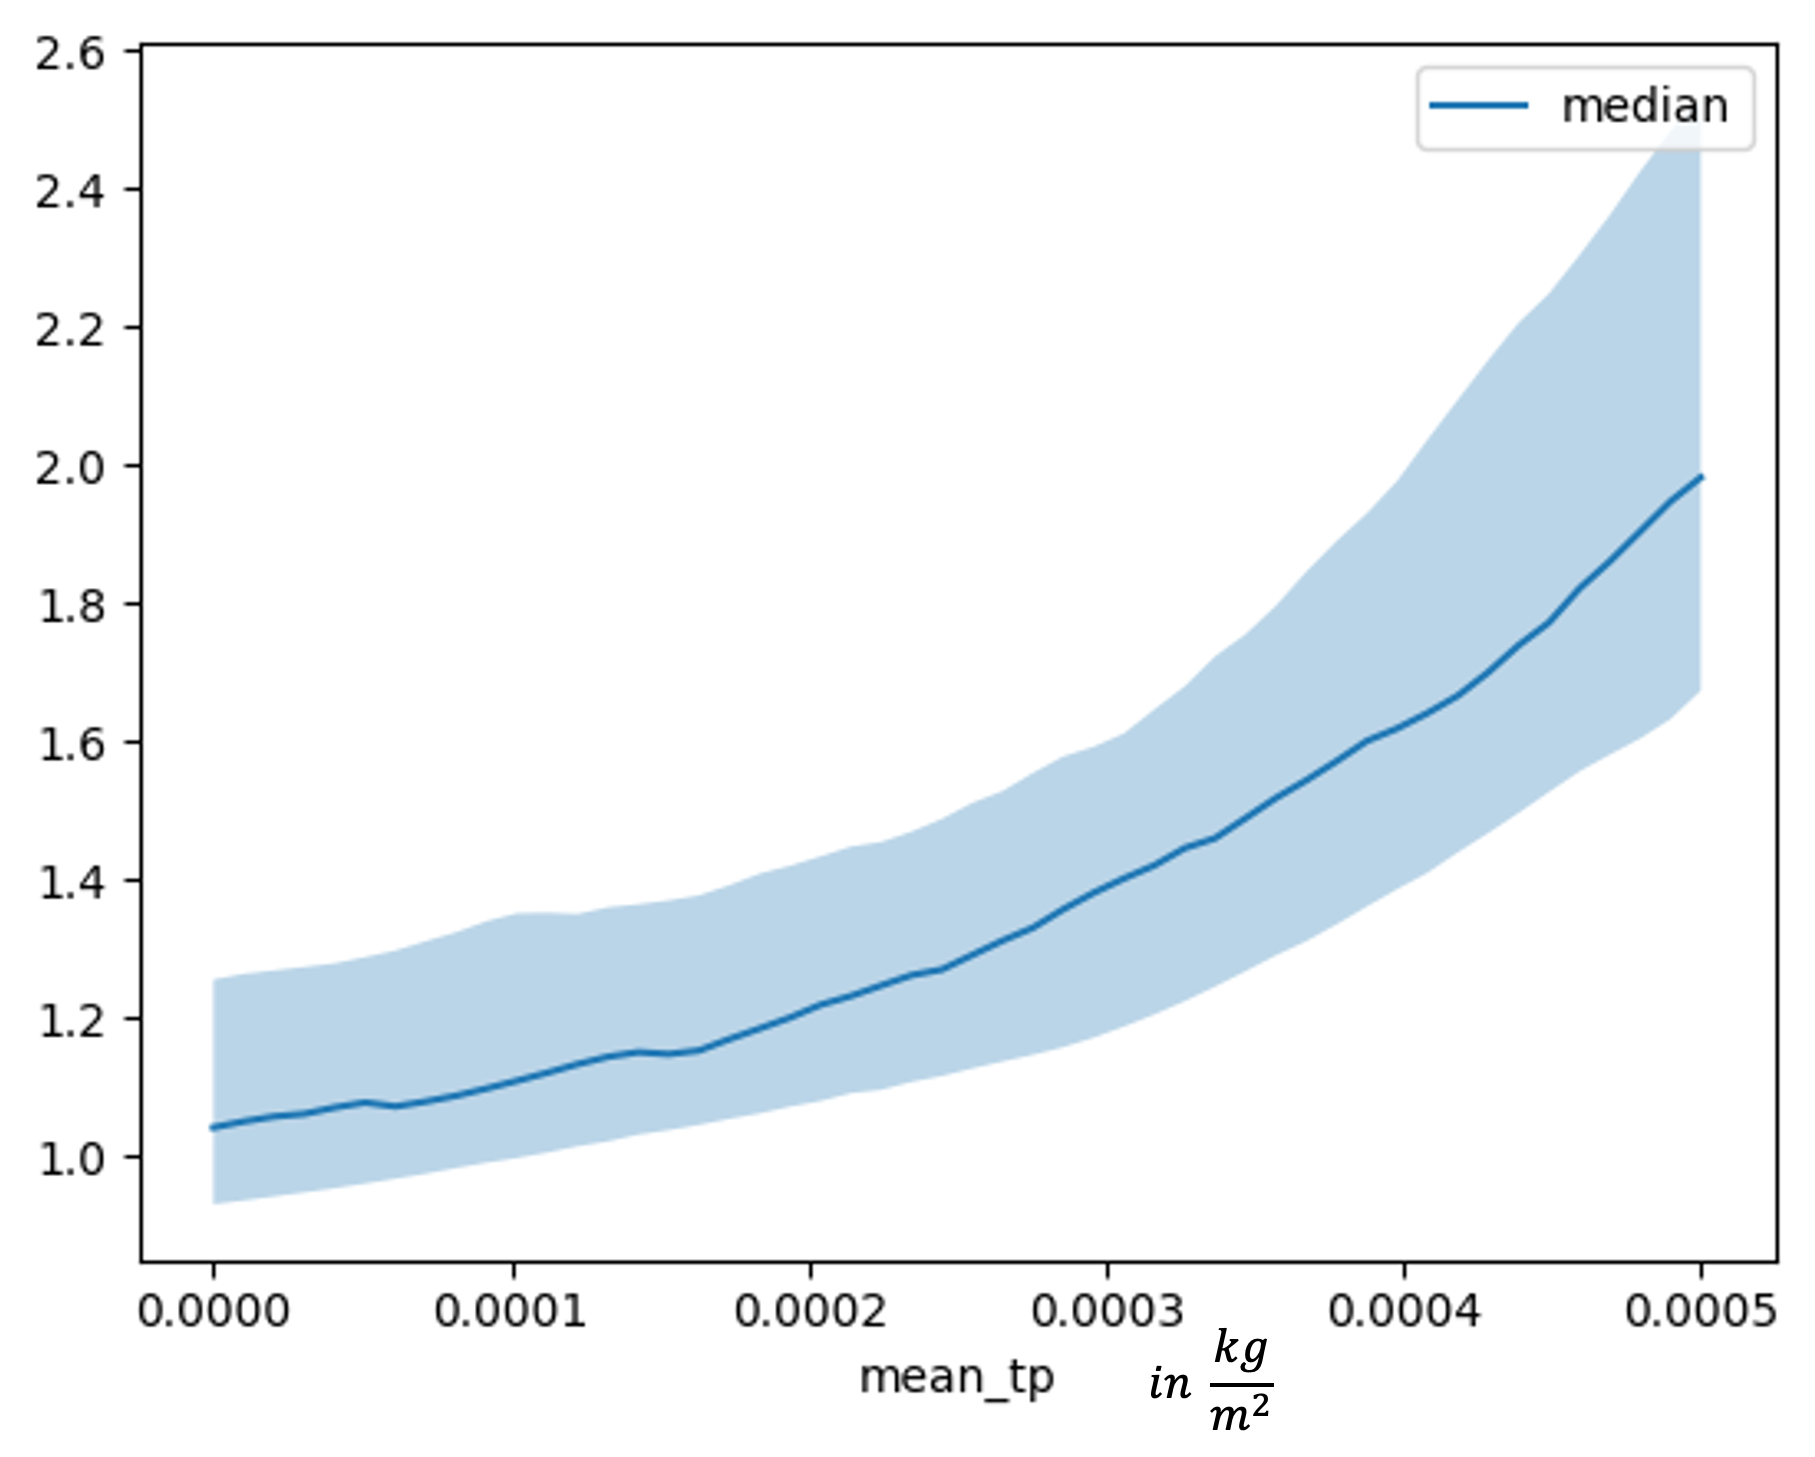
\includegraphics[width=0.7\linewidth]{work/07-hydroLSTM/images/mean_tp_feature_importance_lstm} 

}

\caption{Feature dependence plot for mean total precipitation for a lead time 5 trained LSTM}\label{fig:tp-lstm-imp}
\end{figure}

\begin{figure}

{\centering 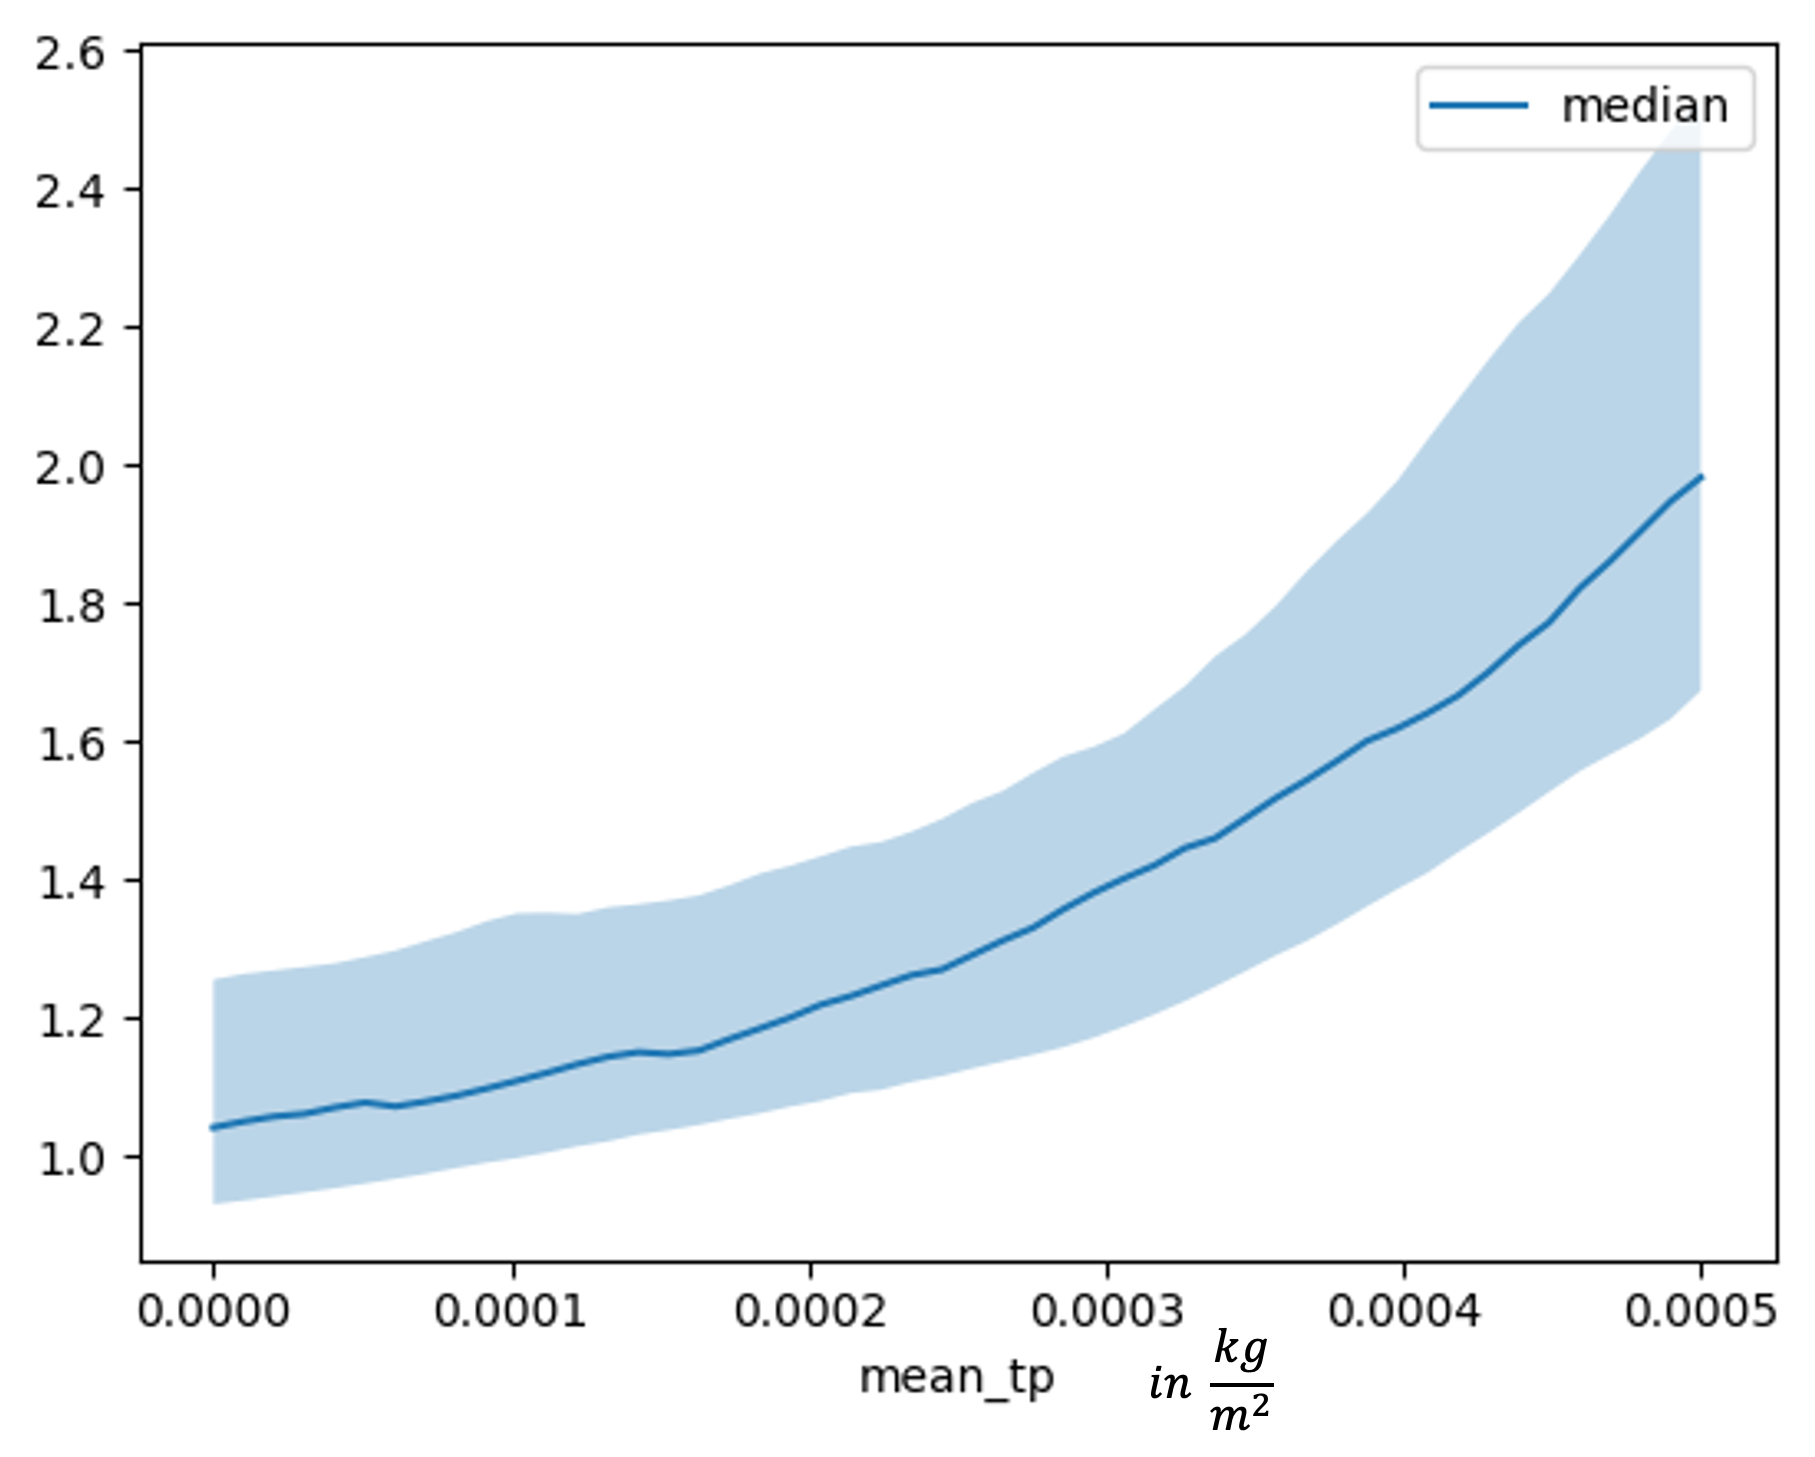
\includegraphics[width=0.7\linewidth]{work/07-hydroLSTM/images/mean_tp_feature_importance_tft} 

}

\caption{Feature dependence plot for mean total precipitation for a lead time 5 trained TFT}\label{fig:tp-tft-imp}
\end{figure}

\begin{figure}

{\centering \includegraphics[width=0.7\linewidth]{work/07-hydroLSTM/images/mean_t2m_feature_importance_lstm} 

}

\caption{Feature dependence plot for mean two meter temperature for a lead time 5 trained LSTM}\label{fig:t2m-lstm-imp}
\end{figure}

\begin{figure}

{\centering \includegraphics[width=0.7\linewidth]{work/07-hydroLSTM/images/mean_t2m_feature_importance_tft} 

}

\caption{Feature dependence plot for mean two meter temperature for a lead time 5 trained TFT}\label{fig:t2m-tft-imp}
\end{figure}

\section{Conclusion}\label{conclusion-4}

This study compares the performance of LSTM (Long Short-Term Memory) and Temporal Fusion Transformer (TFT) models in forecasting streamflows of the bavarian Regen river for up to seven days ahead, using precipitation and temperature as future known covariates alongside historical streamflow data. The data used was obtained from freely available data provided by the Bavarian hydrology authority and Copernicus Climate Project.

The findings indicate that both models exhibit limitations in predicting extreme values such as floods, with KGE (Kling-Gupta Efficiency) scores significantly lower than those reported in similar studies like \citet{sabzipour2023}, likely due to limited data amounts and the challenges inherent in modeling a river system instead of a reservoir. The results also demonstrate a clear difference in performance trends between the two models across different lead times.

Although the KGE was not used as the loss function in training the models. The LSTM's observed KGE scores are high starting at 0.9696 for a one-day lead time, before dropping sharply to 0.3185 for a seven-day lead time. Conversely, the TFT model shows a more gradual decline, from 0.8352 at one day to 0.5717 at seven days, suggesting it maintains more consistent accuracy over longer forecast horizons.

Despite the sharper decline in performance for longer lead times, the LSTM model is notably less resource-dependent, making it a viable option for scenarios where computational resources are limited. However, attempts to forecast streamflows without future known meteorological variables were unsuccessful, underscoring the importance of these covariates in achieving accurate predictions.

While the moving average was applied here, it is not advised to use this tool for streamflow forecasting. By reducing the peaks in the target variable it artificially boosts the predictive abitlity of the model and forces the model to miss the peaks by an even larger margin. In a flood scenario even with a high KGE, the model would miss the exact streamflow value as it was trained on lower peaks and would underestimate the posed danger in the situation.

\section{Outlook}\label{outlook}

Implementing a robust hyper-parameter tuning routine is essential to optimize model performance. This process will require additional computational resources due to the complexity and extensive search space. Given the high dependency of hyper-parameters on lag, it might be necessary to tune hyper-parameters for each lead time separately.

To make the models more sensitive to extreme events such as floods, specialized loss functions could be employed or training a consecutive model that that specifically forecasts the peaks taking the first models predictions as inputs.

The ERA5 dataset used for obtaining meterological data in this study only provides a very coarse representation of the underlying variables. The use of down scaling techniques to obtain a finer grid than the one used in this study might be able to boost the accuracy of the model.

Another next step could be to test the models ability to generalize by training on multiple datasets from different rivers. Including static variables such as river basin properties and land use information can help in creating a more comprehensive model that can adapt to various river systems.

\chapter{The Lancet Report 2023}\label{he1}

\emph{Author: Michael Strobl}

\emph{Supervisor: Prof.~Dr.~Helmut Küchenhoff}

\emph{Suggested degree: Bachelor}

\section{Introduction}\label{introduction-6}

The 2023 report of the Lancet Countdown on health and climate change (\citet{romanello20232023}) aims to monitor the evolving impact of climate change on health and the emerging health opportunities of climate action. It is in its eighth iteration and was created by 114 scientists and health practitioners from 52 research institutions and UN agencies from all continents (but Antarctica). While this chapter is based on the 2023 report, there are also regional reports available, such as the 2024 report for Europe (\citet{Van_Daalen2024-ut}).

The current report focuses on 47 indicators, tracking changes based on observed data as well as projections, in the following fields:

\begin{enumerate}
\tightlist
\item
  Health hazards, exposures, and impacts
\item
  Adaptation, planning, and resilience for health
\item
  Mitigation actions and health co-benefits
\item
  Economics and fincance
\item
  Public and political engagement with health and climate change
\end{enumerate}

The remainder of this chapter provides some background information on climate models, detailed information on three indicators, and a discussion.

\section{Background}\label{background}

Shared Socioeconomic pathways (SSPs) (\citet{RIAHI2017153}) were established by the climate research community in order to make the analysis of future climate impacts, vulnerabilities, adaptation, and mitigation possible. They describe alternative socioeconomic developments regarding their energy, land use, and emissions implications, e.g.~more or less renewable energy vs.~fossil fuels. The following SSPs are of interest for the rest of this chapter:

\begin{enumerate}
\tightlist
\item
  SSP1: Sustainability (low challenges to mitigation and adaption), corresponding to a 2°C emission scenario
\item
  SSP3: Regional Rivalry (high challenges to mitigation and adaptation), corresponding to a 3.7°C emission scenario
\end{enumerate}

These pathways are considered by climate models, e.g.~CMIP6 (\citet{gmd-9-1937-2016}), in order to describe multiple scenarios for climate projections. Figure \ref{fig:cmip6strobl} shows CMIP6 simulations for multiple models and all SSPs. In this chapter, we consider SSP1, representing a sustainable path, and SSP3, representing a non-sustainable path, which humanity is following right now.

\begin{figure}
\includegraphics[width=1\linewidth]{work/08-lancet/figures/cmip6} \caption{CMIP6 climate simulations for SSPs with projections until 2100 (https://www.dkrz.de/en/communication/climate-simulations/cmip6-en/cmip6-acivities-at-dkrz-overview?set\_language=en; accessed on July 10, 2024)}\label{fig:cmip6strobl}
\end{figure}

\section{Selected Indicators}\label{selected-indicators}

We selected three indicators from the first field (Health hazards, exposures, and impacts) with detailed descriptions and outcomes.

\subsection{Indicator 1.1.2: Exposure of vulnerable populations to heatwaves}\label{indicator-1.1.2-exposure-of-vulnerable-populations-to-heatwaves}

Heatwaves have a severe or even life-threatening impact on human health, e.g.~high temperatures can cause heat stroke, heat exhaustion, heat syncope, and heat cramps (see, for example, \citet{doi:10.1161/CIRCULATIONAHA.122.061832} or \citet{chambers2020}). The following variables (among others) can influence mortality: increased risk for older adults (\textgreater65 years of age), low-income countries due to a reduced number of health workers, or pre-existing cardiovascular and chronic respiratory conditions.

This indicator tracks the number of heatwave days and the exposure of vulnerable populations (older adults and infants \textless1 years of age) to heatwaves. A heatwave day is a period of 2 or more days where both the minimum and maximum temperatures are above the 95th percentile of temperatures in 1986-2005.

The following datasets were used for this indicator:

\begin{itemize}
\tightlist
\item
  ERA5 monthly averaged data on single levels (\citet{hersbach2020era5}): World-wide weather data on a lat-lon grid of 0.25 degrees from 1940 onwards.
\item
  ISIMP3b Bias Adjustment dataset (\citet{lange2021isimip3b}): A bias adjusted and downscaled version of the output of CMIP6 climate models with projections up to the year 2100.
\item
  Hybrid gridded demographic data for the world (\citet{Chambers_2020}): Demographics data from 1950-2020 with 5-year population bands and a 0.5 degree grid.
\item
  2020 Revision of World Population Prospects (\url{https://population.un.org/wpp/}): This dataset contains population estimates as well as projections for 237 countries or areas between 1950 and 2100.
\item
  A global downscaled age structure dataset for assessing human impacts of climate change (\citet{briggsdaviddownscaled}): This dataset contains historic population estimates starting in 1970 and projections considering SSP1 and SSP3 in a 0.5 degree grid.
\end{itemize}

Headline Finding:

``In 2013-2022, infants and people over 65 experienced, on average, 108\% more days of heatwave per year than in 1986-2005.''

Figures \ref{fig:heatwaves1infantsstrobl} and \ref{fig:heatwaves1adultsstrobl} show the increase in the number of heatwave days, comparing the time periods 1986-2005 and 2013-2022, for infants and older adults, respectively. This increase (or decrease for Portugal) per country can be calculated, for example, through ERA5 monthly averaged weather data and the hybrid gridded demographics dataset.

\begin{figure}
\includegraphics[width=1\linewidth]{work/08-lancet/figures/indicator_1_1} \caption{Change in number of heatwave days per country for infants, comparing the time periods 1986-2005 and 2013-2022.}\label{fig:heatwaves1infantsstrobl}
\end{figure}
\begin{figure}
\includegraphics[width=1\linewidth]{work/08-lancet/figures/indicator_1_2} \caption{Change in number of heatwave days per country for older adults, comparing the time periods 1986-2005 and 2013-2022.}\label{fig:heatwaves1adultsstrobl}
\end{figure}

The change in the number of heatwave days ranges from approximately -1 in Portugal to 16 in Tajikistan, with only minimal differences between infants and older adults.

Similarly, the ISIMP3b Bias Adjustment dataset combined with the global downscaled age structure dataset can be used to project the change in heatwave days up until the year 2100. Figures \ref{fig:heatwaves2ssp1strobl} and \ref{fig:heatwaves2ssp3strobl} show the projected change in heatwave days for older adults at mid-century (2041-2060) with baseline period 1995-2014. For example, the increase for Venezuela ranges from approximately 88 (SSP1) to 153 (SSP3) heatwave days per year.

\begin{figure}
\includegraphics[width=1\linewidth]{work/08-lancet/figures/indicator_1_3} \caption{Projections of the change in number of heatwave days for older adults per country for SSP1 (under 2 degree scenario) for mid-century (2041-2060) with baseline period 1995-2014.}\label{fig:heatwaves2ssp1strobl}
\end{figure}
\begin{figure}
\includegraphics[width=1\linewidth]{work/08-lancet/figures/indicator_1_4} \caption{Projections of the change in number of heatwave days for older adults per country for SSP3 (3.7 degree scenario) for mid-century (2041-2060) with baseline period 1995-2014.}\label{fig:heatwaves2ssp3strobl}
\end{figure}

\subsection{Indicator 1.1.5: Heat-related mortality}\label{indicator-1.1.5-heat-related-mortality}

This indicator is tracking days with temperatures exceeding safe levels for humans and heat-related mortality. Only older adults are considered.

Similar datasets are used here as for the previous indicator. However, the difficulty arises due to the fact that safe temperatures may vary across regions (see \citet{Honda2014}).

Headline Finding:

``In 2018-2022, people experienced on average 86 days of health-threatening high temperatures annually. 60\% of such temperatures were made more than twice as likely to occur by human-caused climate change.''

Therefore, \citet{Honda2014} created the notion of an Optimum Temperature (OT), at which the mortality is the lowest. Figure \ref{fig:mortalityhondastrobl} shows an example for the Tokyo Prefecture and the period 1972-2008. A smoothing spline with six degrees of freedom was used to model the Relative Risk (RR) for mortality and observed daily maximum temperature data. OT represents the daily maximum temperature where RR is the lowest. RR was used here in order to account for different populations of regions and an RR=1.0 is the reference mortality at around OT, i.e.~the average number of deaths observed when the daily maximum temperature was within the range of the 75th to the 85th percentile for each year.

\begin{figure}
\includegraphics[width=1\linewidth]{work/08-lancet/figures/121_3} \caption{A smoothing spline with six degrees of freedom was used for temperature data from the Tokyo Prefecture and the period 1972-2008, showing the daily maximum temperatures and the Relative Risk (RR) for mortality.}\label{fig:mortalityhondastrobl}
\end{figure}

The shaded area to the right of OT represents temperatures with increased mortality, i.e.~daily maximum temperatures above OT are considered as risky for older adults. The average OT percentile of 47 Japanese prefectures was 83.6, which was used to decide which daily maximum temperatures exceeded safe levels for this indicator. In addition, a distributed lag nonlinear model (\citet{Armstrong2006-mv}) was used to model the increase in mortality (represented by RR) depending on temperature. This model is considered as a response function, which can be used to calculate the RR and therefore the absolute increase of mortality depending on the observed or projected temperatures.

Figure \ref{fig:mortality1strobl} shows the increase in the number of days with unsafe temperatures (daily maximum temperatures exceeding OT). This includes the increasing number of days that were made at least twice as likely due to human induced climate change (it is not described how the red line was created).

\begin{figure}
\includegraphics[width=1\linewidth]{work/08-lancet/figures/indicator_2_1} \caption{Average number of days with unsafe temperatures for older adults from 1997 to 2022, including days that are twice as likely due to climate change.}\label{fig:mortality1strobl}
\end{figure}

In addition, Figures \ref{fig:mortality2ssp1strobl} and \ref{fig:mortality2ssp3strobl} show the absolute projected increase in heat-related mortality per country for older adults at mid-century (2041-2060) compared to 1995-2014 as baseline, for SSP1 and SSP3, respectively. In both cases there is an increase, although it seems that the two scenarios, SSP1 and SSP3, have been flipped accidentially. In addition, only the absolute increase is shown, i.e.~it is obvious that highly populated countries, such as India and China, have a very high increase compared to smaller countries.

\begin{figure}
\includegraphics[width=1\linewidth]{work/08-lancet/figures/indicator_2_4} \caption{Projections of the absolute change in heat-related mortality for older adults per country for SSP1 (under 2 degree scenario) for mid-century (2041-2060) with baseline period 1995-2014.}\label{fig:mortality2ssp1strobl}
\end{figure}
\begin{figure}
\includegraphics[width=1\linewidth]{work/08-lancet/figures/indicator_2_5} \caption{Projections of the absolute change in heat-related mortality for older adults per country for SSP3 (3.7 degree scenario) for mid-century (2041-2060) with baseline period 1995-2014.}\label{fig:mortality2ssp3strobl}
\end{figure}

The response function is kept constant for these projections, i.e.~adaptation is ignored for this indicator. Also, absolute numbers of mortality are used here, i.e.~it was not distinguished between heat-related deaths and other causes.

\subsection{Indicator 1.4: Food insecurity and undernutrition}\label{indicator-1.4-food-insecurity-and-undernutrition}

In 2022, 725 million people faced hunger and in 2021, 3.1 billion people were unable to afford a healthy diet (\citet{noauthor_2023-jt}). For example, climate change is undermining crop yields, affecting labour capacity, and threatening food security of marine resources.

In addition to the previously mentioned datasets, specifically ERA5 and ISIMP3b, data from the Food and Agriculture Organization Food Insecurity Experience Scale (FIES) (\citet{CAFIERO2018146}) was used. This dataset contains survey data from 153 countries and territories during the years 2014, 2015, and 2016. Among others, people were asked for whether they experienced moderate or severe food insecurity within the past 12 months. This was matched with weather data in these peoples specific regions in order to find out whether they experienced heatwaves (as previously defined) or drought months (12-monthly SPEI; only during the growth season of specific crops). In order to make predictions for all other years, including the future, a time-varying panel regression model was used (without further detail). The goal was to predict the percentage of people reporting food insecurity based on heatwaves and drought months experienced within a specific year.

Headline Finding:

``The higher frequency of heatwave days and drought months in 2021 compared to 1981--2010, is associated with 127 million more people experiencing moderate or severe food insecurity.''

Figure \ref{fig:food1strobl} shows world-wide predictions of the change in percentage points (using the previously mentioned model) for heatwaves and drought months for the period 2014-2021. As temperatures, number of heatwave days as well as number of drought months increase, more people are expected to experience severe or moderate food insecurity.

\begin{figure}
\includegraphics[width=1\linewidth]{work/08-lancet/figures/indicator_3_1} \caption{Impact of extreme weather (heatwaves and droughts) on food insecurity from 2014-2021, based on survey data.}\label{fig:food1strobl}
\end{figure}

Figures \ref{fig:food2ssp1strobl} and \ref{fig:food2ssp3strobl} show projections (SSP1 and SSP3, respectively) for the percentage point changes for both kinds of extreme weather combined for mid-century (2014-2060), compared to the baseline 1995-2014. For example for Somalia, this change ranges from 4.02 (SSP1) to 10.32 (SSP3).

\begin{figure}
\includegraphics[width=1\linewidth]{work/08-lancet/figures/indicator_3_2} \caption{Projections of the impact of extreme weather on food inscurity per country for SSP1 (under 2 degree scenario) for mid-century (2041-2060) with baseline period 1995-2014.}\label{fig:food2ssp1strobl}
\end{figure}
\begin{figure}
\includegraphics[width=1\linewidth]{work/08-lancet/figures/indicator_3_3} \caption{Projections of the impact of extreme weather on food inscurity per country for SSP3 (3.7 degree scenario) for mid-century (2041-2060) with baseline period 1995-2014.}\label{fig:food2ssp3strobl}
\end{figure}

It is unclear why for many countries there is missing data.

\section{Discussion}\label{discussion-1}

The 2023 report of the Lancet Countdown on health and climate change provides a comprehensive overview of the current state of the impact of climate change on health and opportunities of climate action. 47 indicators are used to keep track of where humanity is at right now.

We provided detailed descriptions of three main indicators and the modelling techniques used, if mentioned. However, there are a few issues discovered:

\begin{itemize}
\tightlist
\item
  These modelling techniques are typically not described in much detail. Sometimes, as in the case for \citet{Honda2014}, some more information is provided in cited articles, but still on a relatively high level.
\item
  The baselines for comparisons or projections vary. It is not clear, nor described, why different baselines are used. For projections, it is obvious that the baseline for CMIP6 projections (1995-2014) was used, without information on why not the one that was previously used for the indicator at hand.
\item
  In general, the main findings are reported, without going much into detail on how the authors came up with these. In some cases, e.g.~indicator 1.1.5, cited articles provide more information, but in other cases, e.g.~indicator 1.4, it seems to be mainly the authors own work, without providing details.
\end{itemize}

\chapter{Epidemiologic studies on the heat effects}\label{he2}

\emph{Author: Oussama Mesbah}

\emph{Supervisor: Helmut Kuechenhoff}

\emph{Degree: Bachelor}

\section{Introduction}\label{introduction-7}

This chapter covers epidemiologic studies on the effects of heat on health. The aim is to discuss the excess mortality attributed to heat and cold based on recent studies by Masselot et al.~(2023) \citep{masselot2023} and the joint effects of air pollution and heat on mortality as examined by Stafoggia et al.~(2023) \citep{stafoggia2023}.

\section{Excess Mortality Attributed to Heat and Cold}\label{excess-mortality-attributed-to-heat-and-cold}

\subsection{Background for Study}\label{background-for-study}

Masselot et al.~(2023) conducted a comprehensive study on the mortality impacts of non-optimal ambient temperatures. Both heat and cold are established risk factors, and the study aims to provide a robust assessment of these impacts. Previous research has predominantly focused on country-specific data or omitted significant factors.

\subsection{Added Value}\label{added-value}

This study offers several key advancements:

First, it has unprecedented city coverage, examining 854 urban areas across Europe. This extensive coverage offers a more comprehensive assessment compared to prior studies that focused on specific countries or regions. Furthermore, the study balances its focus on both heat and cold impacts, providing a complete picture of temperature-related health risks. It explicitly models age-specific risks and provides age-standardized mortality rates, which allow for fair comparisons across different locations with varying demographic compositions. This is particularly important as it highlights the heightened vulnerability of the elderly population.

Compared to Zhao et al.~(2021) \citep{zhao2021} , Masselot et al.~(2023) focuses on a more detailed regional scope by examining 854 cities in Europe, while Zhao's study covered 750 locations globally. Both studies cover the same period from 2000 to 2019, allowing for direct comparison. Masselot's study utilizes higher resolution ERA5-Land reanalysis data, which may provide a more accurate exposure assessment, especially for smaller cities. Additionally, the inclusion of age-specific mortality data in Masselot's study allows for a more nuanced analysis of age-related vulnerability to temperature extremes. Here is a table summarizing the key differences between the two studies:

\begin{longtable}[]{@{}
  >{\raggedright\arraybackslash}p{(\columnwidth - 6\tabcolsep) * \real{0.1902}}
  >{\raggedright\arraybackslash}p{(\columnwidth - 6\tabcolsep) * \real{0.1902}}
  >{\raggedright\arraybackslash}p{(\columnwidth - 6\tabcolsep) * \real{0.2331}}
  >{\raggedright\arraybackslash}p{(\columnwidth - 6\tabcolsep) * \real{0.3865}}@{}}
\toprule\noalign{}
\begin{minipage}[b]{\linewidth}\raggedright
Feature
\end{minipage} & \begin{minipage}[b]{\linewidth}\raggedright
Zhao et al.~(2021)
\end{minipage} & \begin{minipage}[b]{\linewidth}\raggedright
Masselot et al.~(2023)
\end{minipage} & \begin{minipage}[b]{\linewidth}\raggedright
Added Benefit of Masselot et al.~(2023)
\end{minipage} \\
\midrule\noalign{}
\endhead
\bottomrule\noalign{}
\endlastfoot
\textbf{Geographical Scope} & Global (750 locations in 43 countries) & Europe (854 cities in 30 countries) & More detailed focus on a specific region. \\
\textbf{Temporal Scope} & 2000-2019 & 2000-2019 & Allows direct comparison of results. \\
\textbf{Exposure Data} & Gridded temperature data (0.5° x 0.5°) & ERA5-Land reanalysis data (9 km resolution) & Higher resolution data provides more accurate exposure assessment. \\
\textbf{Outcome Data} & Daily all-cause or non-external mortality counts & Daily all-cause or non-accidental mortality counts, with age-specific data for a subset of cities & Inclusion of age-specific mortality data allows for nuanced analysis. \\
\textbf{Modeling Framework} & Three-stage: time-series regression, meta-regression, prediction & Three-stage: quasi-Poisson regression with DLNM, meta-regression with PLS, kriging interpolation & Incorporation of PLS for dimensionality reduction and kriging for spatial interpolation. \\
\textbf{Vulnerability Assessment} & Limited to 5 meta-predictors & Includes 22 city-specific characteristics & Comprehensive assessment of vulnerability factors. \\
\textbf{Age-Specific Analysis} & Not explicitly mentioned & Provides age-specific relative risks and age-standardized mortality rates & More targeted understanding of vulnerable age groups. \\
\end{longtable}

\subsection{Limitations}\label{limitations}

The study also has limitations. The extrapolation of exposure-response functions (ERFs) across European cities may introduce bias, especially in less-covered areas like Eastern Europe. Additionally, reliable ERFs could not be estimated for people younger than 20 years due to low death counts, limiting the analysis for younger populations.

\subsection{Findings}\label{findings}

The study by Masselot et al.~(2023) provides a detailed analysis of the impact of non-optimal temperatures on mortality across Europe. The study found an annual excess of 203,620 deaths due to cold and 20,173 deaths due to heat. Age-standardized excess death rates were calculated at 129 per 100,000 person-years for cold and 13 per 100,000 person-years for heat.

\subsubsection{Regional Variations}\label{regional-variations}

The results indicated significant variations across different regions of Europe. The highest mortality effects were observed in eastern European cities, where the infrastructure and healthcare systems might be less equipped to handle extreme temperatures compared to their western counterparts.

\begin{figure}
\centering
\includegraphics{work/09-epidemiologic/figures/Bild1.png}
\caption{Relative Risk at Different Temperatures and Ages}
\end{figure}

\subsubsection{Age-Related Vulnerability}\label{age-related-vulnerability}

The study highlighted that vulnerability increases with age, particularly for individuals aged 85 and above. The pooled overall cumulative exposure-response relationship was predicted at several ages: 20-44 years, 45-64 years, 65-74 years, 75-84 years, and 85+ years. This data provides crucial insights into how different age groups respond to temperature extremes.

\begin{figure}
\centering
\includegraphics{work/09-epidemiologic/figures/Bild2.png}
\caption{Relative Risk for Cold and Heat in Capital Cities}
\end{figure}

Several key terms are defined in the study to better understand the results:

\begin{itemize}
\tightlist
\item
  \textbf{Exposure-Response Function (ERF):} This describes the relationship between exposure levels (temperature) and mortality risk.
\item
  \textbf{Minimum Mortality Temperature (MMT):} The specific temperature at which mortality risk is lowest.
\item
  \textbf{Minimum Mortality Percentile (MMP):} The temperature range where the population is generally healthiest.
\item
  \textbf{Relative Risk (RR):} The ratio of mortality risk at a specific temperature compared to the MMT.
\end{itemize}

The study also analyzed the relative risks for cold and heat in capital cities across five age groups. The findings showed that excess mortality is generally lower in Western Europe compared to Northern and Southern Europe.

\subsubsection{Geographical Gradient}\label{geographical-gradient}

One notable finding is the north-south gradient in the Minimum Mortality Percentile (MMP) and Minimum Mortality Temperature (MMT). As temperatures get hotter, the MMP decreases and the MMT increases, indicating that populations in hotter climates have adapted to higher temperatures as their baseline for optimal health.

\begin{longtable}[]{@{}
  >{\centering\arraybackslash}p{(\columnwidth - 2\tabcolsep) * \real{0.5000}}
  >{\centering\arraybackslash}p{(\columnwidth - 2\tabcolsep) * \real{0.5000}}@{}}
\toprule\noalign{}
\begin{minipage}[b]{\linewidth}\centering
\includegraphics{work/09-epidemiologic/figures/Bild5.png}
\end{minipage} & \begin{minipage}[b]{\linewidth}\centering
\includegraphics{work/09-epidemiologic/figures/Bild6.png}
\end{minipage} \\
\midrule\noalign{}
\endhead
\bottomrule\noalign{}
\endlastfoot
Minimum Mortality Temperature Across Europe & Minimum Mortality Percentile Across Europe \\
\end{longtable}

The study's maps illustrate these gradients and the spatial distribution of temperature-related mortality risks. For example, cold-related mortality shows higher excess death rates in Eastern Europe, while heat-related mortality is more prominent in Southern Europe.

\begin{longtable}[]{@{}
  >{\centering\arraybackslash}p{(\columnwidth - 2\tabcolsep) * \real{0.5000}}
  >{\centering\arraybackslash}p{(\columnwidth - 2\tabcolsep) * \real{0.5000}}@{}}
\toprule\noalign{}
\begin{minipage}[b]{\linewidth}\centering
\includegraphics{work/09-epidemiologic/figures/Bild7.png}
\end{minipage} & \begin{minipage}[b]{\linewidth}\centering
\includegraphics{work/09-epidemiologic/figures/Bild8.png}
\end{minipage} \\
\midrule\noalign{}
\endhead
\bottomrule\noalign{}
\endlastfoot
Cold-Related Standardized Excess Death Rate & Heat-Related Standardized Excess Death Rate \\
\end{longtable}

These visualizations provide a comprehensive overview of the temperature-mortality relationship across Europe, highlighting regions and populations that are most vulnerable to extreme temperatures.

\subsection{Conclusion}\label{conclusion-5}

The detailed findings from this study underscore the importance of tailored public health strategies that consider regional and age-specific vulnerabilities. By understanding the nuanced impacts of heat and cold across different European cities and demographic groups, policymakers can better prepare for and mitigate the adverse health effects of extreme temperatures.

\subsection{Data and Framework}\label{data-and-framework}

The study utilized data from 854 urban audit cities from Eurostat and 232 cities from the Multicountry Multi-city (MCC) Collaborative Research Network. City-specific meta-predictors included total population, proportion of population above 65 years, population density, GDP per capita, and environmental factors like PM2.5 concentration and annual temperature range.

Dimensionality reduction is achieved using PLS regression to create composite indices of vulnerability. This method helps in capturing geographical variability in risks while avoiding overfitting. PLS regression is used for dimensionality reduction and predictive modeling, particularly useful when dealing with a large number of highly correlated predictors. The Akaike Information Criterion (AIC) helps select the optimal number of PLS components by balancing goodness of fit with model complexity.

\subsection{Modelling Framework}\label{modelling-framework}

The modelling framework includes several stages:
1. \textbf{City-Specific Risk Estimation:} Using a quasi-Poisson regression model with a distributed lag non-linear model (DLNM).
2. \textbf{Meta-Regression and Spatial Interpolation:} Pooling city-specific estimates into a multivariate multilevel meta-regression model.
3. \textbf{Prediction and Impact Assessment:} Predicting ERFs for all 854 cities and estimating excess deaths.

Here is a Flowchart of the Modelling Framework:

\begin{figure}
\centering
\includegraphics{work/09-epidemiologic/figures/Bild11.png}
\caption{Modelling Framework Flowchart}
\end{figure}

\subsection{Partial Least Squares (PLS) Regression}\label{partial-least-squares-pls-regression}

Partial Least Squares (PLS) regression is a statistical method used for dimensionality reduction and predictive modeling. It is particularly useful when dealing with a large number of highly correlated predictors. The goal of PLS is to find the fundamental relations between two matrices (predictors and responses) by projecting the predictors to a new space.

In the context of epidemiologic studies on the heat effects, PLS regression helps in creating composite indices of vulnerability from city-specific characteristics. This method captures geographical variability in risks while avoiding overfitting.

\subsubsection{PLS Algorithm}\label{pls-algorithm}

The PLS algorithm iteratively constructs new predictor variables (latent variables) that are linear combinations of the original predictor variables. These new variables are uncorrelated and explain the maximum possible variance in the response variables.

The steps involved in PLS are as follows:

\begin{enumerate}
\def\labelenumi{\arabic{enumi}.}
\item
  \textbf{Standardize the predictors and responses}:
  \[
  \mathbf{X} = \frac{\mathbf{X} - \mathbf{\bar{X}}}{\mathbf{S_X}}
  \]
  \[
  \mathbf{Y} = \frac{\mathbf{Y} - \mathbf{\bar{Y}}}{\mathbf{S_Y}}
  \]
\item
  \textbf{Calculate the covariance matrix}:
  \[
  \mathbf{C} = \mathbf{X}^T \mathbf{Y}
  \]
\item
  \textbf{Extract the first latent variable}:
  \[
  \mathbf{w}_1 = \arg \max \left( \mathbf{w}^T \mathbf{C} \mathbf{w} \right)
  \]
  Subject to \(\|\mathbf{w}\| = 1\).
\item
  \textbf{Compute the scores for the first latent variable}:
  \[
  \mathbf{t}_1 = \mathbf{X} \mathbf{w}_1
  \]
  \[
  \mathbf{u}_1 = \mathbf{Y} \mathbf{q}_1
  \]
  Where \(\mathbf{q}_1 = \mathbf{C} \mathbf{w}_1\).
\item
  \textbf{Deflate the matrices}:
  \[
  \mathbf{X}_1 = \mathbf{X} - \mathbf{t}_1 \mathbf{p}_1^T
  \]
  \[
  \mathbf{Y}_1 = \mathbf{Y} - \mathbf{t}_1 \mathbf{c}_1^T
  \]
  Where \(\mathbf{p}_1 = \mathbf{X}^T \mathbf{t}_1 / (\mathbf{t}_1^T \mathbf{t}_1)\) and \(\mathbf{c}_1 = \mathbf{Y}^T \mathbf{t}_1 / (\mathbf{t}_1^T \mathbf{t}_1)\).
\item
  \textbf{Repeat steps 2-5} for the remaining components.
\end{enumerate}

\subsubsection{Geometric View}\label{geometric-view}

Geometrically, PLS regression can be viewed as projecting the original predictor space \(\mathbf{X}\) into a lower-dimensional latent space while maximizing the covariance between the predictors and the responses \(\mathbf{Y}\).

The projections are chosen to ensure that each successive pair of latent variables captures the maximum possible covariance between \(\mathbf{X}\) and \(\mathbf{Y}\).

\begin{figure}
\centering
\includegraphics{work/09-epidemiologic/figures/Bild9.png}
\caption{Geometric View of PLS}
\end{figure}

\subsection{Akaike Information Criterion (AIC) and Model Selection}\label{akaike-information-criterion-aic-and-model-selection}

AIC is used to select the optimal number of PLS components. It balances the goodness of fit with the complexity of the model. Lower AIC values indicate a better model fit, accounting for the number of parameters used.

The formula for AIC is:
\[
\text{AIC} = 2k - 2\ln(\hat{L})
\]
where \(k\) is the number of parameters in the model and \(\hat{L}\) is the maximized value of the likelihood function for the estimated model.

The plot below shows the AIC values for different numbers of PLS components. The optimal number of components is indicated by the lowest AIC value, which in this case is four components. This balance ensures that the model is neither overfitted nor underfitted, providing a parsimonious and explanatory model for predicting temperature-related mortality risks.

\includegraphics{work/09-epidemiologic/figures/Bild12.png} \footnote{Source: Excess mortality attributed to heat and cold}

\subsection{Application in the Study}\label{application-in-the-study}

In the epidemiologic study on the heat effects, PLS regression was performed by reducing the dimensionality of city-specific characteristics into a few uncorrelated components. These components were then used in the meta-regression model to predict temperature-related mortality risks across different cities and age groups.

The PLS regression allowed the study to incorporate a large number of variables, such as demographic and environmental factors, without overfitting the model. This approach provided a robust framework for assessing the vulnerability of different urban areas to heat and cold effects.

By selecting the optimal number of components through AIC, the study ensured that the models were both parsimonious and explanatory, leading to reliable predictions of excess mortality due to temperature extremes.

\subsection{Application in the Study}\label{application-in-the-study-1}

In the epidemiologic study on the heat effects, PLS regression was performed by reducing the dimensionality of city-specific characteristics into a few uncorrelated components. These components were then used in the meta-regression model to predict temperature-related mortality risks across different cities and age groups.

The PLS regression allowed the study to incorporate a large number of variables, such as demographic and environmental factors, without overfitting the model. This approach provided a robust framework for assessing the vulnerability of different urban areas to heat and cold effects.

By selecting the optimal number of components through AIC, the study ensured that the models were both parsimonious and explanatory, leading to reliable predictions of excess mortality due to temperature extremes.

\subsection{Model}\label{model-1}

The model used to estimate the main effect of air temperature on mortality employs a quasi-Poisson regression framework. This framework is suitable for count data, such as daily death counts, and can handle overdispersion commonly observed in such data.\citep{engelhardt2013}

\subsubsection{Quasi-Poisson Regression Model}\label{quasi-poisson-regression-model}

The primary model is formulated as follows:
\[ \text{log}(\mu_i) = \alpha + \sum_{j=1}^{p} \beta_j x_{ij} + \gamma z_i \]
where:
- \(\mu_i\) is the expected daily death count for day \(i\),
- \(\alpha\) is the intercept,
- \(x_{ij}\) represents the predictor variables (e.g., temperature, humidity, etc.) for day \(i\) and predictor \(j\),
- \(\beta_j\) are the regression coefficients for the predictor variables,
- \(z_i\) includes other confounders such as air pollution levels, day of the week, and long-term trends,
- \(\gamma\) represents the coefficients for the confounders.

The quasi-Poisson model is an extension of the Poisson model, which allows for overdispersion by adding a dispersion parameter \(\theta\):
\[ \text{Var}(Y_i) = \theta \mu_i \]

\subsection{Assessing Overdispersion}\label{assessing-overdispersion}

In epidemiological studies involving count data, such as daily mortality counts, it is essential to assess for overdispersion. Overdispersion occurs when the observed variance in the count data is greater than what is expected under a standard Poisson model. This can lead to underestimated standard errors and consequently overconfident statistical inferences.

\subsubsection{Overdispersion in Poisson Models}\label{overdispersion-in-poisson-models}

The Poisson regression model assumes that the mean and variance of the count data are equal (\(\mu = \sigma^2\)). However, in real-world data, this assumption often does not hold, especially in the presence of unobserved heterogeneity or clustering effects.

To assess for overdispersion, we can use the following diagnostic measures:

\begin{enumerate}
\def\labelenumi{\arabic{enumi}.}
\item
  \textbf{Dispersion Parameter (\(\theta\))}:
  The dispersion parameter is defined as the ratio of the Pearson chi-square statistic to the degrees of freedom:
  \[
  \theta = \frac{\sum_{i=1}^{n} (y_i - \hat{\mu}_i)^2 / \hat{\mu}_i}{n - p}
  \]
  where \(y_i\) is the observed count, \(\hat{\mu}_i\) is the predicted count, \(n\) is the number of observations, and \(p\) is the number of parameters estimated in the model. A \(\theta\) value greater than 1 indicates overdispersion.
\item
  \textbf{Pearson Chi-Square Statistic}:
  The Pearson chi-square statistic is calculated as:
  \[
  X^2 = \sum_{i=1}^{n} \frac{(y_i - \hat{\mu}_i)^2}{\hat{\mu}_i}
  \]
  This statistic is compared against the chi-square distribution with \(n - p\) degrees of freedom. A significantly large value indicates overdispersion.
\item
  \textbf{Residual Deviance}:
  The residual deviance should be approximately equal to the degrees of freedom under the Poisson assumption. A much larger residual deviance suggests overdispersion:
  \[
  \text{Deviance} = 2 \sum_{i=1}^{n} \left[ y_i \log\left(\frac{y_i}{\hat{\mu}_i}\right) - (y_i - \hat{\mu}_i) \right]
  \]
\end{enumerate}

\subsubsection{Addressing Overdispersion}\label{addressing-overdispersion}

When overdispersion is detected, alternative modeling approaches should be considered to obtain valid statistical inferences:

\begin{enumerate}
\def\labelenumi{\arabic{enumi}.}
\item
  \textbf{Quasi-Poisson Model}:
  The quasi-Poisson model adjusts for overdispersion by introducing a dispersion parameter:
  \[
  \text{Var}(Y_i) = \theta \mu_i
  \]
  This model provides robust standard errors that account for overdispersion.
\item
  \textbf{Negative Binomial Model}:
  The negative binomial model is another approach that introduces an additional parameter to model the overdispersion. The variance is modeled as:
  \[
  \text{Var}(Y_i) = \mu_i + \alpha \mu_i^2
  \]
  where \(\alpha\) is the overdispersion parameter. This model is particularly useful when the overdispersion increases with the mean.
\item
  \textbf{Generalized Estimating Equations (GEE)}:
  GEEs provide a flexible approach to handle correlated and overdispersed data by specifying a working correlation structure. They produce robust standard errors that are valid even if the specified correlation structure is incorrect.
\end{enumerate}

\subsubsection{Application in the Study}\label{application-in-the-study-2}

In the context of the study on the effects of temperature on mortality, assessing overdispersion is crucial for ensuring the validity of the model estimates. The quasi-Poisson regression model was chosen for this study due to its ability to handle overdispersed data effectively. The dispersion parameter was estimated, and diagnostic checks were performed to confirm the presence of overdispersion.

By using the quasi-Poisson model, the study obtained robust standard errors and more reliable estimates of the temperature-mortality relationship. This approach ensured that the findings were not biased by underestimated variability, leading to more accurate and confident public health recommendations.

\subsubsection{Quasi-Poisson Regression Model}\label{quasi-poisson-regression-model-1}

The Quasi-Poisson regression model adjusts for overdispersion in count data like mortality. The model is represented as:
\[ \text{log}(\mu_i) = \alpha + \sum_{j=1}^{p} \beta_j x_{ij} + \gamma z_i \]
where \(\mu_i\) is the expected daily death count, \(\alpha\) is the intercept, \(x_{ij}\) represents the predictor variables (e.g., temperature), \(\beta_j\) are the regression coefficients, and \(z_i\) includes other confounders like air pollution levels.

\subsubsection{Distributed Lag Non-Linear Model (DLNM)}\label{distributed-lag-non-linear-model-dlnm}

To capture the delayed and non-linear effects of temperature on mortality, a Distributed Lag Non-Linear Model (DLNM) is used \citep{gasparrini2010}. The DLNM incorporates the lagged effects of temperature, recognizing that exposure to extreme temperatures can affect mortality over several days. The model can be expressed as:
\[ \text{log}(\mu_i) = \alpha + f(\text{temperature}_{i-l}) + \sum_{k} \beta_k z_{ik} \]
where \(f(\text{temperature}_{i-l})\) represents a smooth function of temperature over lag \(l\) days, and the other terms are as previously defined.

The smooth function \(f\) is typically modeled using splines, allowing for flexible non-linear relationships:
\[ f(\text{temperature}_{i-l}) = \sum_{m=1}^{M} s_m(\text{temperature}_{i-l}) \]
where \(s_m\) are the spline basis functions and \(M\) is the number of basis functions.

\subsubsection{Meta-Analysis}\label{meta-analysis}

In the second stage, the results from individual city-specific models are pooled using a multilevel random-effects meta-analysis. This approach combines the estimates from different cities while accounting for between-city variability. The random-effects model is given by:
\[ \hat{\theta}_j = \theta + u_j + \epsilon_j \]
where:
- \(\hat{\theta}_j\) is the estimated effect size for city \(j\),
- \(\theta\) is the overall effect size,
- \(u_j\) is the random effect for city \(j\), assumed to follow a normal distribution with mean 0 and variance \(\tau^2\),
- \(\epsilon_j\) is the within-city error term.

The overall effect size \(\theta\) is estimated by weighting the city-specific estimates based on their variances:
\[ \hat{\theta} = \frac{\sum_{j=1}^{J} w_j \hat{\theta}_j}{\sum_{j=1}^{J} w_j} \]
where \(w_j = \frac{1}{\text{Var}(\hat{\theta}_j) + \tau^2}\) are the weights.

\subsubsection{Incorporating Age-Specific Effects}\label{incorporating-age-specific-effects}

The model also considers age-specific effects by stratifying the analysis by different age groups. Age-stratified models help in understanding the differential impact of temperature on various age cohorts. The age-specific model is given by:
\[ \text{log}(\mu_{i,a}) = \alpha_a + \sum_{j=1}^{p} \beta_{j,a} x_{ij} + \gamma_a z_i \]
where \(\mu_{i,a}\) is the expected daily death count for age group \(a\), and the other terms are as previously defined but specific to age group \(a\).

\subsection{Findings and Interpretation}\label{findings-and-interpretation}

The combination of quasi-Poisson regression, DLNM, and multilevel meta-analysis provides a robust framework for estimating the temperature-mortality relationship. The pooled estimates across cities indicate the overall effect of temperature on mortality while accounting for local variations and confounders.

The findings from the model underscore the significant impact of temperature extremes on mortality, with cold temperatures generally showing a larger effect than heat in many European cities. The results highlight the importance of considering both immediate and lagged effects of temperature, as well as the need for city-specific and age-specific analyses to inform targeted public health interventions.

By employing these advanced statistical techniques, the study provides comprehensive and nuanced insights into the public health implications of temperature variability and extreme weather events.

\section{Joint Effect of Heat and Air Pollution on Mortality}\label{joint-effect-of-heat-and-air-pollution-on-mortality}

\subsection{Findings}\label{findings-1}

The study by Stafoggia et al.~(2023) examined the combined effects of high temperatures and air pollution on mortality. The analysis involved data from 620 cities in 36 countries, providing a comprehensive overview of the joint impact of these environmental stressors. The findings indicated that both high temperatures and air pollution independently increase mortality rates. However, their combined effect is significantly more pronounced. Specifically, a temperature increase from the 75th to the 99th percentile was associated with an 8.9\% rise in mortality.

\subsection{Model}\label{model-2}

To estimate the joint effect of air temperature and air pollution on mortality, a two-stage modeling approach was employed.

\subsubsection{First Stage: City-Specific Models}\label{first-stage-city-specific-models}

In the first stage, city-specific models were developed using a quasi-Poisson regression framework. The model is expressed as:

\[ \text{log}(\mu_{i}) = \alpha + \beta_1 \text{Temp}_{i} + \beta_2 \text{PM}_{i} + \beta_3 (\text{Temp}_{i} \times \text{PM}_{i}) + \sum_{j=1}^{p} \gamma_j z_{ij} \]

where:
- \(\mu_{i}\) is the expected daily death count for day \(i\),
- \(\alpha\) is the intercept,
- \(\text{Temp}_{i}\) represents the temperature on day \(i\),
- \(\text{PM}_{i}\) represents the air pollution level (e.g., PM2.5 concentration) on day \(i\),
- \(\text{Temp}_{i} \times \text{PM}_{i}\) is the interaction term between temperature and air pollution,
- \(\beta_1, \beta_2,\) and \(\beta_3\) are the coefficients for temperature, air pollution, and their interaction, respectively,
- \(z_{ij}\) represents other covariates (e.g., day of the week, long-term trends),
- \(\gamma_j\) are the coefficients for the covariates.

The interaction term (\(\beta_3\)) captures the joint effect of temperature and air pollution on mortality, indicating how the combined exposure amplifies the risk.

\subsubsection{Distributed Lag Non-Linear Model (DLNM)}\label{distributed-lag-non-linear-model-dlnm-1}

The DLNM was used to account for the delayed effects of temperature and air pollution. The model is formulated as:

\[ \text{log}(\mu_{i}) = \alpha + f(\text{Temp}_{i-l}, \text{PM}_{i-l}) + \sum_{k=1}^{p} \gamma_k z_{ik} \]

where:
- \(f(\text{Temp}_{i-l}, \text{PM}_{i-l})\) is a bivariate smooth function of temperature and air pollution over lag \(l\) days,
- \(z_{ik}\) are other covariates.

This model allows for flexible modeling of the non-linear and lagged relationships between temperature, air pollution, and mortality.

\subsubsection{Second Stage: Meta-Analysis}\label{second-stage-meta-analysis}

In the second stage, the city-specific estimates were pooled using a multilevel random-effects meta-analysis. This approach combines the results from different cities, accounting for between-city heterogeneity.

The random-effects model is given by:

\[ \hat{\theta}_j = \theta + u_j + \epsilon_j \]

where:
- \(\hat{\theta}_j\) is the estimated effect size for city \(j\),
- \(\theta\) is the overall effect size,
- \(u_j\) is the random effect for city \(j\), assumed to follow a normal distribution with mean 0 and variance \(\tau^2\),
- \(\epsilon_j\) is the within-city error term.

The overall effect size \(\theta\) is estimated by weighting the city-specific estimates based on their variances:

\[ \hat{\theta} = \frac{\sum_{j=1}^{J} w_j \hat{\theta}_j}{\sum_{j=1}^{J} w_j} \]

where \(w_j = \frac{1}{\text{Var}(\hat{\theta}_j) + \tau^2}\) are the weights.

\subsection{Comparison of Findings: Masselot et al.~(2023) vs.~Stafoggia et al.~(2023)}\label{comparison-of-findings-masselot-et-al.-2023-vs.-stafoggia-et-al.-2023}

Both studies highlight the significant impact of temperature on mortality, but they approach the analysis from different angles and include different additional variables.

\subsubsection{\texorpdfstring{Masselot et al.~(2023) \citep{masselot2023}}{Masselot et al.~(2023) {[}@masselot2023{]}}}\label{masselot-et-al.-2023-masselot2023}

\begin{itemize}
\tightlist
\item
  \textbf{Focus}: Assessed the impact of non-optimal temperatures (both heat and cold) on mortality across Europe.
\item
  \textbf{Model}: Used a quasi-Poisson regression with DLNM for temperature effects, and meta-regression for pooling city-specific estimates.
\item
  \textbf{Key Findings}: Higher mortality rates associated with cold temperatures compared to heat. Significant regional variations with Eastern Europe showing higher vulnerability. Age-specific analysis revealed increased vulnerability in older age groups.
\item
  \textbf{Data}: Included 854 cities across Europe.
\end{itemize}

\subsubsection{\texorpdfstring{Stafoggia et al.~(2023) \citep{stafoggia2023}}{Stafoggia et al.~(2023) {[}@stafoggia2023{]}}}\label{stafoggia-et-al.-2023-stafoggia2023}

\begin{itemize}
\tightlist
\item
  \textbf{Focus}: Examined the joint effect of high temperatures and air pollution on mortality.
\item
  \textbf{Model}: Used a quasi-Poisson regression with an interaction term for temperature and air pollution, combined with DLNM for lagged effects. Pooled city-specific estimates using multilevel random-effects meta-analysis.
\item
  \textbf{Key Findings}: Both high temperatures and air pollution independently increase mortality, but their combined effect is more pronounced. The interaction between temperature and air pollution significantly amplifies mortality risk.
\item
  \textbf{Data}: Included 620 cities in 36 countries.
\end{itemize}

\subsubsection{Comparison of Temperature Effects}\label{comparison-of-temperature-effects}

\begin{itemize}
\tightlist
\item
  \textbf{Temperature Alone}:

  \begin{itemize}
  \tightlist
  \item
    Both studies confirm that temperature extremes (both high and low) significantly affect mortality rates.
  \item
    Masselot et al.~focused on a broad spectrum of temperature effects, including both heat and cold.
  \item
    Stafoggia et al.~specifically addressed the interaction between heat and air pollution.
  \end{itemize}
\item
  \textbf{Combined Effects}:

  \begin{itemize}
  \tightlist
  \item
    The interaction term in Stafoggia et al.'s model revealed a synergistic effect, where the combined exposure to heat and air pollution resulted in a higher mortality risk than the sum of their individual effects.
  \item
    This aspect was not covered in Masselot et al.'s study, which did not include air pollution as a variable.
  \end{itemize}
\item
  \textbf{Methodological Differences}:

  \begin{itemize}
  \tightlist
  \item
    Masselot et al.~used a wider range of temperatures and focused on a comprehensive assessment of cold and heat effects, including age-specific vulnerabilities.
  \item
    Stafoggia et al.~provided insights into the compounded effects of environmental stressors, emphasizing the need to consider multiple factors in public health policies.
  \end{itemize}
\end{itemize}

\subsection{Conclusion}\label{conclusion-6}

Both studies contribute valuable insights into the public health impacts of temperature extremes. Masselot et al.~(2023) \citep{masselot2023} highlighted the broader spectrum of temperature effects across Europe, while Stafoggia et al.~(2023) \citep{stafoggia2023} provided a nuanced understanding of the combined effects of heat and air pollution. Together, these studies underscore the importance of considering both direct and interactive effects of environmental stressors in epidemiological research and public health planning.

\chapter{Controversial issue : heat and humidity}\label{he3}

\emph{Author: Mona Niethammer}

\emph{Supervisor: Helmut Kuechenhoff}

\emph{Degree: Master}

\section{Abstract}\label{abstract-5}

As climate change progresses, heat-related mortality and adverse health outcomes are also increasing. In the chapters before it was mainly talked about temperature related outcomes. This chapter focuses on heat events and how humidity plays a crucial role in high ambient temperatures and the effect on health outcomes. Physiological research indicates that both heat and humidity significantly impact the body's response to heat. Thus, influencing mortality and adverse health outcomes. Several epidemiological studies aimed to show this relationship, found however only minimal or even no effect of humidity on negative health outcomes. This discrepancy between physiological knowledge and epidemiological findings creates a, as (\citet{baldwin2023}) describes it, controversial issue. This will be further explored in this chapter.

\section{Introduction}\label{introduction-8}

\subsection{Background}\label{background-1}

Climate change is a broad and pressing topic as the number of heat-related deaths and the air-temperature break records. Extreme heat waves have become a consistent feature of summer seasons, leading to an increase in heat-related fatalities (\citet{ebi2021}). Rising greenhouse gas concentrations further contribute to rising temperatures and humidity at the same time. Physiological knowledge indicates that heat and humidity both contribute to human heat stress, adversely affecting the human body (\citet{baldwin2023}). Heat stress occurs when environmental conditions overwhelm the body`s cooling mechanism (\citet{buzan2020}). When the body is not able to sufficiently lower its core temperature, the human body suffers health problems, potentially leading to death. From a physiological perspective, the body's cooling mechanisms are clearly influenced both by heat and humidity.

In contrast, a wide range of epidemiological studies have found either no or only a weak correlation between humidity and human heat stress or adverse health outcomes. Those studies all infer that a rise in air-temperature (heat) is associated with negative health outcomes. These two contradictions lead, according to (\citet{baldwin2023}), to a controversial issue as physiologically it is known that there is an effect of humidity on health outcomes, whereas in epidemiological studies they did not find evidence for such an effect. Figure 1 describes this contradiction between physiological knowledge and epidemiological studies. Heat in this chapter is used as synonym for high ambient temperature.

\begin{center}\includegraphics[width=0.8\linewidth]{Controversial Issue} \end{center}

\textbf{Figure 1:} Flowchart illustrating the controversial issue between epidemiological studies and physiological knowledge.\\
\emph{A: illustrates how heat and humidity changes with climate change. B: illustrates that epidemiological studies only take heat as driver into account, the physiological view heat and humidity. C: shows the predictions from an epidemiological and physiological view.}

\subsection{Epidemiological Studies}\label{epidemiological-studies}

Numerous epidemiological studies investigated the influence of heat and humidity on negative health outcomes such as death or cardiovascular diseases. Results of these studies are mixed regarding the association of humidity and negative health outcomes. As an example, a study in New York, conducted by Barreca found a positive correlation between high levels of relative humidity (RH) and cardio-respiratory hospitalizations. However, this study is one of few that identified an effect of humidity on negative health outcomes.
Baldwin et al.~reviewed several epidemiological studies and conducted further research. They concluded six key reasons why epidemiological studies found less or even no effect of humidity on health outcomes:

\begin{enumerate}
\def\labelenumi{\arabic{enumi})}
\tightlist
\item
  At high temperatures, humidity has minimal or even no influence on negative health outcomes\\
\item
  Study results may be skewed by limited data sets\\
\item
  Analyses often focus on vulnerable populations, like elderly, infants or individuals with impaired sweating functions\\
\item
  Necessary extreme values of heat and humidity to show a significant impact on heat strain are rare\\
\item
  The relationship between heat and humidity is often not adequately considered. This may lead to inappropriate model results\\
\item
  Sub-daily meteorological phenomena, such as rain, which occur during high heat and humidity, may bias studies based on daily data\\
  (\citet{baldwin2023}).
\end{enumerate}

\subsection{Physiological knowledge}\label{physiological-knowledge}

Physiological evidence indicates that heat and humidity increase health risks, leading to higher rates of morbidity, mortality, reduced physical work capacity, and other adverse health outcomes as the climate crisis worsens. (\citet{buzan2020})

The human body has two primary cooling mechanism to control the body temperature. One mechanism redistributes the blood flow to the skin (vasodilation), and therefore allows metabolically generated heat from inside of the body to reach the skin's surface and subsequently the environment. This process requires an increased blood flow and elevates cardiac demand. This may trigger cardiovascular events such as myocardial infarction in subjects with heart conditions.
The second mechanism involves secreting sweat onto the skin. Subsequently, the sweat evaporates to the environment and heat from the body is removed. These two mentioned cooling mechanisms are crucial for the human body to maintain a sustainable core temperature. (\citet{ebi2021})

The effectiveness of these cooling mechanisms decline with the increase of heat and humidity. A higher ambient humidity reduces the proportion of sweat that evaporates from the skin into the air. Hence, the effectiveness of sweating decreases and sweating does not lead to heat loss anymore, causing a rise in body temperature. The human body responds to such ineffective sweating by an even higher rate of sweating. This can lead to heat stroke, dehydration, or the body's physical limits may simply be exceeded. (\citet{baldwin2023})

Certain populations are at higher risk due to less efficient cooling mechanisms. For instance, people older than 65 years may have a reduced sweating ability same as individuals with cardiovascular diseases who cannot effectively increase blood flow to the skin. These factors, among others, exacerbate the difficulty in cooling the body. (\citet{ebi2021})\\
When the body can no longer cool itself, heat stress occurs. However, these physiological insights are not consistently reflected in epidemiological studies. Several methodological and physiological factors might explain this discrepancy.

Firstly, heat-vulnerable individuals often have impaired sweating capacities, especially with aging this capacity decreases. Thermoregulatory sweating can decrease by up to 25\% in individuals older than 60. Consequently, they will be less sensitive to high humidity. Since most studies only include individuals over 65 years, this might explain the lack of association between humidity and heat stress.

Secondly, it is possible that the threshold at which differences in humidity impact the body's regulatory mechanisms are rarely attained. This means, that only at a specific threshold of humidity the body's cooling mechanisms have trouble and this threshold may be reached rarely in especially dry areas.

Thirdly, heat-related outcomes may result from other causes unrelated to humidity. For example, cardiovascular diseases are a leading cause of death, and high temperatures can exacerbate these conditions independently of humidity.

Lastly, dehydration, a major cause of heat-related deaths, reduces the amount of sweat, thereby minimizing the impact of high humidity on evaporation and cooling. (\citet{baldwin2023})

\section{Heat and Humidity in Studies}\label{heat-and-humidity-in-studies}

\subsection{Humidity definitions}\label{humidity-definitions}

Humidity has multiple definitions. This makes it crucial to select an appropriate measure to answer specific research questions. (\citet{baldwin2023}) categorize humidity variables into the four following groups:

\begin{enumerate}
\def\labelenumi{\arabic{enumi}.}
\tightlist
\item
  Simple relative variables including Relative Humidity (RH), Dew-point depression (DPD) and Saturation deficit.\\
\item
  Mass-based variables including specific humidity, absolute humidity, dew point temperature, vapor pressure and mixing ratio.\\
\item
  Composite indicators such as the Heat index, Humidex, Wet-bulb-temperature, UTCI and further more.\\
\item
  Physiologic-based humidity indicators including maximum evaporation, required evaporation, total evaporation.
\end{enumerate}

The simple relative variable RH (\%) is the ratio of actual vapor pressure (e) in the air to the saturation vapor pressure (\(e_s\)), indicating proximity to saturation (\(RH=e/e_s\)). The dew-point depression (DPD) (°C) indicates the relative dryness of the air and is the difference between the near-surface air temperature (\(T_a\)) and the dew point temperature (\(T_d\)) (\(DPD=T_a-T_d\)). Saturation deficit refers to the amount by which the water vapor must be increased in a given environment to reach saturation, assuming unchanged temperature and pressure.

The mass-based variable specific humidity (q) (g/kg) is the ratio of the mass of water vapor (g) to the total mass of moist air (kg). Absolute humidity is the density of water vapor, defined as the ratio of the mass of water vapor (g) to the volume of the air mixture (\(m^3\)). The dew point temperature (\(T_d\)) (°C) is the temperature at which saturation occurs. The mixing ratio (w) refers to the ratio of the mass of water vapor (g) to the mass of dry air (kg).

The Heat Index (HI) describes a ``feels like'' temperature, while the Humidex is a discomfort index. The wet-bulb temperature is the temperature at which air becomes saturated through evaporation at constant pressure. The Universal Thermal Climate Index (UTCI) (°C) is a physiologically based thermal stress scale designed to reflect the average human physiological response to the outdoor thermal environment.

The physiological-based humidity indicator maximum evaporation (\(E_{max}\)) represents the maximal evaporation rate in a given environment and clothing conditions. The required evaporation (\(E_{req}\)) measures the evaporation needed to achieve thermal balance, and the total evaporation (E) is the total amount of heat lost via evaporation of sweat from the body.

Davis et al.~reviewed the use of humidity variables in epidemiological studies. They found that 62\% of the studies used RH, while absolute and specific humidity were used in only 5.3\% and 1.5\% of the studies, respectively. They discussed the appropriate use of different humidity variables, especially the use of RH due to its strong inverse correlation with temperature and its diurnal and seasonal variability was mentioned. It is recommended to use RH sparingly. Instead, they recommend using mass-based variables such as absolute or specific humidity, as they provide a more accurate measure of exposure to humidity levels.\\
The selection of humidity variables must be done carefully, they can be highly correlated with other variables, for example with heat. Davis et al.~concluded that using RH as humidity variable is often inappropriate and should be done with caution if necessary. (\citet{davis2016})

The widespread use of RH in epidemiological studies is largely caused by the available data and the measurements which are performed. Mostly, if humidity is measured, then RH is measured. Deriving mass water-vapor based variables such as absolute and specific humidity can introduce uncertainty and bias in estimates.

\subsection{Composite Indicators}\label{composite-indicators}

Composite indicators are frequently used in studies. There are over 120 heat stress metrics available (\citet{buzan2020}), most of which were originally designed for heat warning systems. Composite indicators consider heat, humidity, and additional variables simultaneously, making them practical for certain applications. Often they are just a weighted sum of different variables. Using such composite indices is very practical, but it comes at the cost of interpretability. Changes in the composite index can result from variations in heat, humidity, or other included variables. Therefore, information about individual effects is lost and the effects can not be separated. Furthermore, the use of such indices may lead to biased or misleading estimates. Hence, the effects of heat or humidity may be underestimated. Baldwin et al.~recommend the use of alternative methods such as confounding or effect modification, to separately assess the effects of heat and humidity (\citet{baldwin2023}).

\subsection{Confounder}\label{confounder}

A confounder is a variable that affects both the exposure of interest and the outcome. Figure 2 illustrates how humidity acts as a confounder in the relationship between heat and health outcomes.

\begin{center}\includegraphics[width=0.8\linewidth]{Confounder} \end{center}

\textbf{Figure 2:} Humidity as confounding effect.

Humidity has been used in many epidemiological studies as a confounder when the effect of heat on health outcomes was analyzed. Researchers aim to remove the confounding influence of humidity on the relationship between heat and health outcomes by adjusting for humidity. This means the indirect effect of humidity through heat will be eliminated. Not adjusting for confounder variables, the causal effect of heat may be overestimated. This adjustment leads to a different interpretation of the estimates, as shown in the following linear model:

\[
Ε[Y│t,h]= β_0+ β_1*t+ β_2*h
\]

Y represents the health outcome of interest, t is heat, and h humidity. In this model, \(β_1\) represents the conditional total effect of heat on the health outcome at any given level of humidity. \(β_2\) represents the direct effect of humidity on the outcome. That is the causal effect of humidity on the outcome when heat is held fixed and thus blocking the humidity effect on heat.

Interpretation of estimates can however get very complex and sometimes even misleading.Consequently, the causal relation between the variables needs to be considered carefully (\citet{baldwin2023}, \citet{westreich2013})

One significant problem of adjusting for confounding is to potentially run into multicollinearity issues.
If heat (the exposure of interest) and humidity (the confounder) are highly correlated and both variables are included in the same regression model multicollinearity is present. Consequently, the estimates capture similar information and therefore making it difficult to interpret individual variable effects. Additionally, the precision of the estimated coefficients may be reduced. Including further variables such as calendar variables to adjust for long-term or seasonal trends can exacerbate multicollinearity if the correlation between heat and humidity varies significantly over time. Furthermore, including other variables which are highly correlated with heat and humidity will lead to further multicollinearity issues.

Baldwin et al.~suggest using alternative approaches to significance testing that do not rely solely on p-values. Furthermore, it is crucial to carefully consider the relationship between heat and humidity and their individual effects on health outcomes to avoid misleading results. (\citet{baldwin2023})

\subsection{Effect Modification and Interaction}\label{effect-modification-and-interaction}

Including humidity as an effect modifier or interaction with heat is another method to test an effect of humidity in the framework of negative health outcomes and was used in some epidemiological studies (\citet{baldwin2023}). Unlike confounding, which distorts relationships and should therefore be eliminated, effect modification and interaction are desirable biases. They provide valuable insights into how variables interact and influence outcomes, revealing inherent aspects of causal relationships that need clarification.

Often, the two terms \emph{Effect Modification} and \emph{Interaction} are used interchangeably. However, from a causal view these two concepts differ in a counterfactual perspective and slightly differ in their definition. The counterfactual perspective involves hypothetical scenarios, asking ``What if?'' questions such as, ``What if heat remained the same but humidity was lower? Would the health outcome change?''. (\citet{bours2021}) Counterfactual outcomes are typically written with a superscript such as \(Y^t\) and answers the question: ``What would the outcome Y be if the exposure was t?''. Or as another example \(Y^{th}\) answers the question: ``What would the outcome Y be if both exposures t and h occurred together?''. As in real-world data typically not all combinations of exposures are observed in each individual we are talking about hypothetical scenarios.\\
Both concepts are scale dependent and their presence depends on the scale used. Here, we use the risk difference scale for formal definitions.

\emph{Interaction} refers to the combined causal effect of two exposures, such as heat and humidity. \emph{Effect modification} pertains to how the causal effect of one exposure changes across different levels of a second exposure. For example, ``How does the effect of heat change across different levels of humidity?''.
Let T refer to heat, H to humidity and Y represent the outcome of interest such as heat-related death. \(Y^t\) is the counterfactual outcome under exposure t and \(Y^{th}\) is the counterfactual outcome under t and h.

Humidity (H) is \textbf{effect modifier} on the risk difference scale for the effect of heat (T) on the outcome (Y) if H is not affected by T and there are two levels of T (\(t_0\),\(t_1\)) and two levels of H (\(h_0\),\(h_1\)), such that:

\[
Ε[Y^{t_1}│H=h_1] - E[Y^{t_0}│H=h_1] ≠ E[Y^{t_1}|H=h_0]- E[Y^{t_0}|H=h_0]
\]

Effect modification indicates that the effect of heat on the outcome differs across different levels of humidity. By recognizing effect modification, public health interventions can better address how heat exposure interacts with humidity. This enables more targeted strategies to mitigate and adapt health risks associated with specific combinations of heat and humidity.

There is an \textbf{interaction} on the risk difference scale between heat (T) and humidity (H) on the outcome (Y) if there are two levels of T (\(t_0\),\(t_1\)) and two levels of H (\(h_0\),\(h_1\)), such that:
\[
Ε[Y^{t_1, h_1}] - E[Y^{t_0, h_1}] ≠ E[Y^{t_1, h_0}]- E[Y^{t_0, h_0}]
\]

Interaction requires that the joint effect of heat and humidity is different from the sum of their individual effects. If interaction is present, studying each exposure separately may not fully capture the complexity of their joint influence on the outcome. (\citet{vanderweele2009})

According to Baldwin and colleagues, analytical approaches to estimate interaction of effect modification are similar. They suggest that by including interaction terms or effect modifiers the main question of interest needs to be considered same as the scale of interest and the potential policy implications. (\citet{baldwin2023})

Unfortunately, the interpretation of interaction terms and effect modifiers often leads to misinterpretation and often the scale (multiplicative or additive) also is not considered correctly. Therefore, it is crucial to understand the concepts of interaction and effect modification and how to interpret them correctly.

\subsection{Data Limitations}\label{data-limitations}

The availability and quality of weather data vary across different locations all over the world. Low-income countries, like for example most african regions, often have limited access to weather data compared to high-income countries due to limited resources for data collection. Figure 3 illustrates global sub-daily weather data from the HadISD data source. This highlights the inconsistency in data coverage. Many regions in Africa, South America, and Australia have few measurements compared to Europe or the US. Such a lack of data, especially in areas prone to extreme heat events leaves gaps in our understanding and estimation of weather-related impacts on health outcomes.

Tropical and subtropical climates are characterized by high levels of humidity and heat. Unfortunately, these climates are particularly affected by these data limitations. Missing data in tropical and subtropical regions hinder our ability to comprehend the combined effects of heat and humidity on health outcomes. Therefore, epidemiological studies often do not include locations where humidity plays a significant role due to these data gaps.

Another challenge is the temporal resolution of weather data. Many studies rely on daily mean measurements, which may overlook fluctuations in heat and humidity throughout the day. It is known that heat and humidity fluctuate throughout the day. Using daily mean measurements may underestimate the effects of heat and humidity. Furthermore, correlations between heat and humidity can vary depending on the time of day, potentially impacting the findings of epidemiological studies.

Furthermore, typically weather stations are situated outside urban areas, often at airports. This may not capture urban heat effects. Additionally, as most measurements are taken outdoors, indoor and outdoor variations in heat and humidity are not accounted for.

Another limitation is that typically only relative humidity (RH) is measured at weather stations. This may not provide the most accurate representation of humidity. Deriving mass-based variables like specific or absolute humidity from RH may introduce uncertainties and bias in the estimates as menioned earlier.

In summary, the lack of weather data can result in an underestimation of the impact of humidity on health outcomes. Researchers should consider these data limitations, especially when generalizing results to different countries and weather conditions. (\citet{baldwin2023})

\begin{center}\includegraphics[width=0.8\linewidth]{hadisdimage1} \end{center}

\textbf{Figure 3:} Station coverage and length of record in HadISD (\citet{raymond2024})

\section{Examples}\label{examples}

Armstrong et al.~conducted a study to assess the impact of heat and humidity on daily mortality during summer months. They used a time series regression model with a distributed lag nonlinear model (DNLM) for heat, using data from 445 cities across 24 countries. Numerous different models were fitted, including different humidity levels and terms and further one model with an interaction term between heat and humidity was modeled. Model comparison using the Akaike information criterion (AIC) revealed that the best fit was achieved when humidity was included as a linear term, i.e., as confounder. One very surprisingly result was that a 23\% increase in relative humidity at the 99th percentile was associated with a 1.1\% decrease in mortality. This was a non-significant finding contrary to the expectation that humidity leads to an increase in mortality. Sensitivity analyses involving specific humidity and dewpoint yielded similar results. Considering humidity as a potential effect modifier, by including an interaction term, was not favored based on AIC criteria (\citet{armstrong2019}).

Baldwin et al.~criticize solely rely on AIC to determine whether an interaction term should be included in the model. Consequently, as no interaction term was used in the final model, the influence remains uncertain and raises questions about the value of its exclusion. The final model used by Armstrong et al.~included relative humidity as a linear term, thereby treating humidity as a confounder. As highlighted earlier, employing humidity as a confounder can introduce several challenges.

Armstrong et al.recognized some limitations of their study. They discussed the data gaps from tropical and less developed countries, the exclusive consideration of mortality as an endpoint, and the possibility of missing the association between humidity and mortality under specific conditions (\citet{armstrong2019}).

In another epidemiological study from Schwartz et al.~the effect of heat and humidity on hospital admissions for heart disease and myocardial infarction among individuals over 64 years from 12 US cities was investigated. They fitted a Poisson model for each city, incorporating regression splines to control for season and barometric pressure, and adjusting for the day of the week. Despite their broad approach, they found no evidence of an effect of humidity on hospital admissions. Possible explanations for this results are the use of relative humidity and the resulting bias. Further, considering humidity as a confounder may also explain that no effect of humidity was found. Additionally, focusing solely on individuals older than 64, who are more vulnerable to heat and sweating impairments, may have biased the study's findings. (\citet{schwartz2004})

Barreca conducted a study that found an effect of heat and humidity on mortality rates in the US. He used data from the Global Summary of the Day (GSOD) files, which provide detailed weather station data. The study analyzed data from 1973 to 2002, calculating specific humidity using a standard meteorological formula based on mean dew point and mean station pressure.

To estimate the effects of heat and humidity, Barreca employed an ordinary-least-squares model with the following equation:

\[
MORT_{cmy} = \sum_b \beta^b*TEMP^b_{cmy} + \sum_{b'} \alpha^{b'} * HUMID^{b'}_{cmy} + X_{cmy} \gamma + \mu_{my} + \\
\phi_{cm} + \delta_{cm} * TIME + \pi_{cm}*TIME^2 + \epsilon_{kym}
\]

In this model:

\begin{itemize}
\tightlist
\item
  MORT represents the monthly mortality rate (per 100,000 inhabitants) in county c, year y and calendar month m.
\item
  TEMP is a set of temperature variables indicating the fraction of days county c experiences mean temperatures within specific 10 °F bins (e.g., 50--60 °F).
\item
  HUMID is a set of humidity variables indicating the fraction of days county c experiences mean humidity levels within specific two-grams-of-water-vapor bins (e.g., 2--4 g/kg).
\item
  X is a vector of controls for precipitation and temperature-humidity interaction terms.
\item
  \(\mu\) represents unrestricted time effects.
\item
  \(\phi\) represents unrestricted county by calendar month fixed effects.
\item
  \(\delta_{cm}*TIME\) and \(\pi_{cm} * TIME^2\) represent unrestricted county by calendar month quadratic time trends.
  Barreca clustered the standard errors by the state of residence to account for the possibility that
  \(\epsilon\) is correlated within states, both across counties and over time. Additionally, the equation was weighted by the county population in 2000.
  He fitted different models: one model included only temperature, and another included only humidity. Both the temperature-mortality and humidity-mortality relationships followed a similar pattern. In a subsequent model, he included both TEMP and HUMID covariates. An interesting finding from this model was that both cold temperatures and low humidity levels remained significant determinants of mortality.
  Finally, he fitted a model with an interaction term between heat and humidity. The estimates from this model suggest that increasing humidity levels are more dangerous at high temperatures.
  Therefore, controlling for humidity is according to Barreca particularily important in the context of predicting distributional effects of climate change. (\citet{barreca2012})
\end{itemize}

In a separate review, Budd examined the history and limitations of the wet-bulb globe temperature (WBGT) index, widely used since its development for the United States Army and Marine Corps in 1950. The index incorporates air temperature, mean radiant temperature, absolute humidity, and air movement as basic elements of the thermal environment. Budd identifies several limitations of the index, including its underestimation of stress in environments with restricted evaporation, challenges in interpreting its results, and limitations in the accuracy of sweat measurement due to calibration methods and instrumentation. (\citet{budd2008})

\section{Discussion}\label{discussion-2}

The discrepancies observed in epidemiological studies regarding the impact of humidity on health outcomes may stem from various factors. It is important to understand how to appropriately use humidity in study designs and recognize the different humidity definitions. Prioritizing mass water-vapor based variables such as specific or absolute humidity over relative humidity is a crucial step.
As discussed earlier, humidity can be considered as a confounder, effect modifier, in an interaction term with heat or component of a composite index. Each of these considerations of humidity comes with its own set of limitations.

It is essential to provide a clear research question or hypothesis when evaluating the role of humidity in studies. Researchers must be mindful of these considerations to ensure the robustness and validity of their study results.

Efforts to improve data collection are required, especially to include regions with tropical climates and low-income countries that are often underrepresented in studies. Additionally, relying solely on vulnerable populations may introduce bias, underscoring the importance of striving for a representative sample.

Humidity represents an intriguing factor worth studying further, along with heat, especially in studies investigating health effects. Planning and executing appropriate studies to examine the effects of heat and humidity requires a nuanced understanding of humidity. It is appropriate incorporation into models, and knowledge aware of potential limitations and errors.

\chapter{Risk Projections}\label{he4}

\emph{Author: Author}

\emph{Supervisor: Helmut Kuechenhoff}

\emph{Degree: Bachelor}

In many studies, the effects of climate change in the future is discussed.
In a tutorial paper (\citet{vicedo}) , statistical methods for modelling future risks due to climate devlopement are presented. In a two other papers paper the future effects of ozone and heat related are presented (\citet{domingo},\citet{chen}).

\chapter{Climate Crisis and Mental Health}\label{menh3}

\emph{Author: Nina Straub}

\emph{Supervisor: Helmut Küchenhoff}

\emph{Degree: Master}

\section{Introduction}\label{introduction-9}

It is widely recognized that climate change (CC) is impacting both economy and society. However, it is also increasingly acknowledged as critical factor influencing various aspects of human health. In 2009, the World Health Organisation (WHO) declared CC as one of the largest threads to human health of the twenty-first century and recognised the need for a research agenda to understand complex linkages between climate change and health (\citet{worldhealthorganization2009}). In following years, initiatives such as the Lancet Countdown, a global monitoring system designed to track research and support policy decisions on Health and CC, drew resources and attention to this pressing problem (\citet{watts2018}). Despite these efforts, some health conditions are still little researched and the impact of climate change on them is poorly understood. Among them are mental health (MH) and human well-being (\citet{romanello2023}).
According to the OECD, 20-30\% of the working population are affected by a MH condition. Mental disorders are the worldwide leading cause of years lived with disability (\citet{whiteford2013}, \citet{hewlette2014}) and a considerable burden not only for individuals but also society and economy. In 2010, the direct and indirect costs were estimated to amount to 2493 billion US dollars worldwide (\citet{hewlette2014}) and the lost economic value amounts to 4-8\% of GDP in different regions (\citet{arias2022}). However, health care systems spend a disproportional amount on treatment. In England, MH conditions make out about 26\% of the burden of disease, but only 13\% of health expenditure are attributed to treatment (\citet{hewlette2014}). Globally, 80\% of people do not get sufficient treatment at all (\citet{worldhealthorganization2021}).
Given the proportion of MH in global burden of disease, it seems surprising that little research has investigated how CC might affect MH. The aim of this chapter is to outline the challenges in researching the impact of CC on MH and to present research approaches on this topic. Emphasis will be placed on the methodological and statistical difficulties.

\section{Challenges of Quantifying Climate Change Impact on Mental Health}\label{challenges-of-quantifying-climate-change-impact-on-mental-health}

Important to notice is that CC does not directly impact MH, but rather the consequences of a changing climate, like the increase in magnitude, frequency and intensity of extreme climate events mediate the effect of CC on MH (\citet{hayes2018}). The Intergovernmental Panel On Climate Change (IPCC) report identified multiple pathways how CC could impact MH. The direct pathway includes exposure to traumatic events such as floods, hurricanes or other severe weather-related events. The indirect pathway consists of the consequences of prolonged events such as drought or sea level rise that lead to displacement, food shortages or economic hardship. The last pathway, vicarious exposure or overarching/diffuse exposure refers to the long-term emotional distress caused by the awareness of the negative consequences of CC and the associated feelings of helplessness and despair (\citet{intergovernmentalpanelonclimatechange2023}).
Although in the IPCC report most of the adverse effects of CC on MH are assessed with ``very high confidence'', no concrete projections are given as to how many additional people will suffer from mental disorders. This is peculiar because for other health effects that are assessed with very high confidence, figures for additionally affected individuals are given (\citet{intergovernmentalpanelonclimatechange2023}).
The discrepancy between confidence and tangible figures is caused by multiple challenges of attributing CC to MH, which can be clustered in external and internal difficulties. The external difficulties of quantification mainly consist of the globally insufficient resources devoted to monitoring and treating MH. Although the Lancet Countdown emphasised the need to integrate MH in future CC health considerations, only five out of 16 countries included MH in their health adaption plans (\citet{watts2018}). In the most recent Countdown report it was noted that the development of an indicator to cover the relations between CC and MH is still ongoing (\citet{romanello2023}). One major problems hereby is that current prevalence estimates for mental illnesses are unreliable, as mental illness is severely underdiagnosed, especially in third world countries (\citet{worldhealthorganization2021}). With the lack of a baseline, good projection estimates are difficult.
The internal difficulties of quantification evolve around the complex nature of MH itself. \citet{hayes2018} identified four key aspects which complicate the estimation of CC impact: Firstly, the risk of pathologizing normal stress responses due to a changing climate while adverse mental health outcomes are underdiagnosed. Secondly, multiple causal pathways in which one CC correlate can influence different MH outcomes. Thirdly, effects of CC may only become apparent after a considerable time period, which complicates the investigation of causal effects. Lastly, existing complex interactions between MH and other social determinants of health, and their relationship with CC, is insufficiently understood.

\begin{figure}

{\centering \includegraphics[width=0.8\linewidth]{work/12-mentalhealth/figures/drought_impact} 

}

\caption{Causal process diagram of the impact of drought on the mental health outcomes depression, anxiety and suicide. Numbers in brackets are number of papers meeting the search criteria for each factor. Figure adapted from @vins2015.}\label{fig:impactDrought}
\end{figure}

The four aspects can be illustrated by a causal process diagram, shown in Figure \ref{fig:impactDrought}, which depicts the multiple pathways by which droughts can influence MH outcomes (\citet{vins2015}). Most apparent is the economic route: Droughts have a negative impact on crop yield, influencing employment and financial stability in the agricultural sector. Financial hardship has been shown to have a negative impact on MH, leading to depression and, in severe cases, even suicide (\citet{carleton2017}, \citet{edwards2015}). Another causal route is the one concerned with the decreased availability of food, leading to dietary changes or famine. This can directly influence neurodevelopment of children or anxiety in adults, but also indirectly cause migration, which can lead to social isolation and loss of cultural identity, again having a negative impact on MH outcomes. To estimate the impact of droughts on MH e. g. via the migration route, it would require not only to estimate the increase and severity of droughts due to CC, but also how much migration this would cause and how many of the affected individuals would consequently develop a mental illness. This is a genuine challenge for accurate climate projections, as estimation of migration movements and the development of mental illness depend on many interrelated factors (\citet{mazhin2020}). Some individual linkages between events (e. g. the influence of economic hardship on MH) are well-researched. Future research needs to integrate these pathways and link them to different climate scenarios to better understand the overall causal processes and make accurate projections possible (\citet{vins2015}).

\section{Data Sources and Methods Used to Investigate Climate Change Impact}\label{data-sources-and-methods-used-to-investigate-climate-change-impact}

To enable evidence-based policies to protect health from climate change, the WHO has identified five research priorities: (i) Assessing risks with data-based studies and, in a second step, projections and modelling, (ii) identifying the most effective interventions, (iii) guiding health-promoting mitigation and adaption decisions in other sectors, (iv) improving decision-support and (v) estimating costs (\citet{worldhealthorganization2009}).
While this research agenda has advanced in relation to some health outcomes, research on MH and CC is almost exclusively concerned with the first step of the first priority (\citet{cianconi2020}). Methods used to describe future MH risks vary, but most quantitative studies can be grouped into a few broad categories relating to the data and measurement instruments, the study design and the statistical analysis applied (\citet{charlson2021}). The two main data sources are either official statistics or (representative) surveys. Official statistics such as mortality data or hospitalisation rates are low in cost for the researcher and have the advantage of being more objective than self-assessment questionnaires or interviews. But there are some considerable downsides. Some health outcomes, e. g. suicide rates, are often underreported, especially in countries where there is high stigmatisation. Furthermore, proxy variables sometimes have to replace variables of interest. For example, when examining the impact of drought on farmer suicide rates, occupation is not captured in the mortality statistics and one is limited to analysing rural males aged 30-60 years, assuming that they are working in agriculture (\citet{carleton2017}). Surveys do not have this downside, as one can collect variables of interest and potential confounders directly, leading to more fine-grained information (\citet{edwards2015}). However, survey data is more prone to self-selection bias and dropouts, particularly in longitudinal designs (\citet{kessler2008}). In addition, measuring instruments can have a low validity and data collection is costly in terms of both time and monetary resources. Which data source is chosen is largely dependent on the research question and study design.
The most common study designs are cross-sectional, followed by case-studies. Little studies attempt to model outcomes (\citet{charlson2021}).
The specific statistical analysis depends on the data source and the study design. Classic linear regression (in case of a continuous outcome, e. g. general wellbeing) and logit models (in case of binary outcome, e. g. has a mental illness -- does not have a mental illness) are most often used, but also more flexible models, allowing for non-linear effects of climatic covariates such as temperature or precipitation, are possible.
For a more detailed review on studies about environmental exposure and MH outcomes, see \citet{charlson2021}.
It can be summarized that research concerning the impact of CC on MH is less advanced than research on other health outcomes and mostly restricted to assessing risks. A methodological difficulty inherent to research questions regarding MH is firstly the measurement of MH outcomes, relying on psychometric instruments or diagnostic interviews, and secondly the large number of potential unmeasured confounders, especially when working with official statistics.
An important motivation for researching the interactions between CC and health is that, based on a good understanding of causality and reliable projections, evidence-based measures can contribute to the adaptation of health care systems and prevent the most adverse outcomes. However, in the most frequently used cross-sectional studies on CC and MH, causal interpretations must be carefully scrutinised, particularly when dealing with complex causal processes. Different designs such as longitudinal or interventional designs, a shift towards the other WHO research priorities ii)-v) and a greater focus on non-western regions and populations may contribute to a more reliable, causal understanding.

\section{The Impact of Hurricanes on Posttraumatic Stress Disorder (PTSD)}\label{the-impact-of-hurricanes-on-posttraumatic-stress-disorder-ptsd}

To illustrate how the above theoretical principals are operationalised in practice, an exemplary study and its results will be described in the following. The paper ``Trends in Mental Illness and Suicidality after Hurricane Katrina'' (\citet{kessler2008}) is concerned with the impact of one of the most destructive natural catastrophes in the history of the United States (\citet{graumann2006}). To investigate the effect on MH, 815 pre-hurricane residents of the most affected areas were interviewed 5-8 months after the event (baseline) and again one year later (follow-up). In these interviews, data on hurricane-related stressors, demographic variables (age, gender, ethnicity, household income, education, etc.) and different MH conditions (anxiety and mood disorders, PTSD, suicidality, severity of mental illness) were collected. As the first screening interview found that individuals with higher hurricane-related stress levels chose to not participate in the study, weights were applied to the baseline hurricane-related stress variable to account for this selection bias. Additionally, the authors differentiated between individuals from the New Orleans Metropolitan area (metro subsample) and individuals from other areas (non-metro subsample). Multiple logistic regression models of the form

\[
\pi_i = P(Y_i = \text{mental illness} \mid \eta_i) = h(\eta_i) = \frac{\exp(\eta_i)}{1 + \exp(\eta_i)}
\]
with linear predictors

\[
\eta_i = \beta_0 + \beta_1 x_{i1} + \beta_2 x_{i2} + \cdots + \beta_p x_{ip}
\]

were used to investigate the different outcomes of mental illnesses. In the following, only the results of the outcome of PTSD shall be outlined.
The overall prevalence of PTSD was high in both subsamples and on both measurement points (14.9\% on baseline, 20.9\% on follow-up for the total sample), compared to the US-wide prevalence of 6\% (\citet{goldstein2016}). A two-tailed, within-responded paired t-test showed that prevalence increased significantly over time. Significance was driven by increase of prevalence in the non-metro subsample (11.8 vs 20.0\%, \emph{p} \textless{} 0.001), while the prevalence of the metro-subsample stagnated over time (25.9 vs 24.1\%, \emph{p} = 0.37). Recovery rate in the follow-up was low as 66.4\% of baseline cases continued to have PTSD, 16.9\% classified for another diagnosis and only 16.7\% recovered. In the logistic regression model, only two of the demographic variables, participants age and family income, had a significant influence on PTSD outcome.
The authors hypothesised that the significant increase in prevalence might be explained by an increase in hurricane-related stress. However, this hypothesis was not confirmed by the data. Regarding hurricane-related stress as outcome variable, one can find that stress decreased significantly over time in the whole sample (91.7 vs 57.5\%, \emph{p} = 0.001), but in the follow-up, stress was significantly higher in the metro subsample than the non-metro subsample (78.3 vs 51.7\%, \emph{p} \textless{} 0.001). This contrasts with the increase of PTSD in the non-metro subsample. One can conclude that higher levels of residual hurricane-related stress cannot explain the increase of PTSD prevalence over time in the non-metro subsample. In turn, when taking hurricane-related stress of the follow-up into the model as a predictor variable, one can find that it is indeed significant for both subsamples. In this final model, stress exposure was a key predictor which explained substantial variation in PTSD. The results can be seen in Table \ref{tab:tabResults}. Remarkable are the odds-ratios of 20.3 for severe and 12.8 for serious stress compared to individuals with no hurricane-related stress, after controlling for socio-demographic variables and diagnosis of PTSD in the baseline interview. The authors argue that, if interpreted causally, the population-attributable risk proportion of PTSD due to hurricane-related stress is 31.9\%, meaning that this proportion would be expected to remit if all hurricane-related stress would be resolved. Although the causality assumption may not be fulfilled, this statement is interesting as it could be a methodological approach to estimate additional PTSD diagnoses due to natural disasters.

\begin{table}

\caption{\label{tab:tabResults}Effects of hurricane-related stress on PTSD outcome as shown in @kessler2008.}
\centering
\begin{tabular}[t]{l|l|l}
\hline
Severity & OR & CI\\
\hline
Severe & 20.3* & (4.9–84.6)\\
\hline
Serious & 12.8* & (3.0–53.7)\\
\hline
Moderate & 4.4* & (1.2–16.1)\\
\hline
Mild & 3.5 & (1.0–12.6)\\
\hline
None & 1.0 & \\
\hline
\$\textbackslash{}chi\textasciicircum{}2\$ (\$p\$-value) & 21.0 & (< .001)\\
\hline
\end{tabular}
\end{table}

\emph{Note.} CI, confidence interval; OR, odds ratio; PTSD, posttraumatic stress disorder. Effects estimated with multiple logistic regression model controlling for sociodemographic variables, baseline value of PTSD and subsample. Reference category were participants with no hurricane-related stress. Significance level was 0.05.

The study has four mayor limitations: First, in addition to the mentioned selection bias after the first screening, the dropout rate between measurement points was 21.9\%. Although a weight was used to account for the selection bias, it is possible that other, non-collected variables might influence participation or dropout. Second, only screening scales instead of diagnostic interviews were used for diagnosis. Hurricane-related stress was measured using self-assessment questionnaires, which is both subjective and retrospective and possibly biased by current emotional functioning. Third, although interpreted causally, hurricane-related stress and PTSD might be influenced by unmeasured common causes, influencing the observed association. Lastly, there is no true pre-hurricane baseline for the sample, and preexisting mental illness was not recorded in the survey.
The results of the presented study are partially contradicting similar studies which found a decline in PTSD over time (\citet{chen2015}). The authors hypothesise that the increase in prevalence in the non-metro subsample may be caused by greater media attention and resources being allocated to the New Orleans metropolitan region, leading to a sense of neglect and slower reconstruction of infrastructure in other areas. It is also remarked that other stressors only indirectly linked to the hurricane, such as economic stress or displacement, might influence MH outcomes. This is an interesting point of discussion, as it shows that the IPCC categorization of climate change exposures impacting MH is not as simple as outlined before. Events that fall into the category of direct exposure, such as hurricanes, might have prolonged effects on mental health outcomes, e. g. via economic hardship. This in turn makes it very difficult to attribute MH outcomes to specific CC events, as effects can be observed directly after the event, but can also have a prolonged onset. The potential causal pathways of short-term and long-term stressors on PTSD are depicted in Figure \ref{fig:DAGHurricane}.

\begin{figure}

{\centering \includegraphics[width=0.75\linewidth]{work/12-mentalhealth/figures/DAG_hurricane} 

}

\caption{Potential direct and indirect causal pathways through which hurricanes might influence the development of posttraumatic stress disorder (PTSD).}\label{fig:DAGHurricane}
\end{figure}

To conclude, the study shows that disaster-related stress does play a significant role in PTSD outcome. Since adverse effects are only weakly related to socio-demographic variables, efforts for sufficient treatment must extend to the entire population. High residual hurricane-related stress after two years and its strong relation to PTSD emphasizes the need for evidence-based measures to address residual stress in multiple ways, ranging from rebuilding infrastructure to providing counselling and financial support.
Although the study itself does not link the results to CC, it would be possible to draw a connection between this single, natural disaster and future CC impact on MH. According to the \citet{intergovernmentalpanelonclimatechange2023}, hurricanes are projected to increase in frequency and severity. If, as claimed in the study, hurricane-related stress plays a causal role in the development of PTSD, this increase in hurricanes would have a considerable effect on the number of individuals suffering from PTSD and would need to be taken into account for future health care adaption plans.

\section{Adaption and Mitigation Strategies}\label{adaption-and-mitigation-strategies}

Although the IPCC classifies the adverse impact of CC on MH to be of very high confidence, little attention has been directed to mitigation and adaption strategies for mental health and treatment systems (\citet{charlson2021}). In \citet{berry2018}, a possible approach to deal with the high complexity of the matter is outlined. They criticise that today's policies and epidemiological research is focused mainly on individual outcomes, proximate causes and measurements on short timescales. To address the impact of CC on MH more holistically, they propose ``systems thinking'', which they define as a set of skills used to examine interacting factors that produce outcomes, predict their behaviour and design interventions. More precisely, in research they demand a mixture of CC projections and experimental designs to understand causal influences. In policy, behaviour change should be accomplished through social policy and collective actions instead of aiming at individuals. In direct actions and interventions, they demand a shift from the single-hazard perspective of e. g. extreme weather events to a strategic long-term planning accounting for an increase in those extreme events (\citet{berry2018}).
An example for system thinking would be the protection of infrastructure to benefit MH. This sounds far-fetched, but considering that the cost of damage to critical infrastructure is estimated to increase tenfold (\citet{forzieri2018}), and that these costs divert resources from public health, put pressure on the functioning of society and take up individual resources -- all factors that have a negative impact on MH -- infrastructure protection could be a promotional strategy to protect MH from the impact of CC. The causal diagram of this process is depicted in Figure \ref{fig:DAGInfra}.

\begin{figure}

{\centering \includegraphics[width=0.75\linewidth]{work/12-mentalhealth/figures/DAG_infra_2} 

}

\caption{Top-level process diagramm depicting linkages between climate change, infratructure and mental health, as shown in @berry2018.}\label{fig:DAGInfra}
\end{figure}

The proposal by \citet{berry2018} is a broad framework that may be useful to approach most of the problems discussed in this chapter. However, the individual components are yet to be tested in future research and policy designs.
On the more practical side, \citet{hayes2018} and \citet{newnham2020} proposed several practical measures that could protect MH from direct and indirect CC impact. For acute response to disaster, first-aid responders and nurses need to be trained in basic psychological first aid. It has also proven beneficial for subsequent MH outcomes to prepare people living in vulnerable areas (e.g.~near rivers that will flood more frequently in the future) for the possibility that the event might occur (\citet{munro2017}). Intermediate adaption could include capacity building for therapy and counselling, education and programmes to reduce stigma as well as community-building and preparation training for extreme weather-related events (\citet{newnham2020}). Long-term prevention and mitigation require governments to include MH in their strategic health planning and the development of tools to predict risks, costs and needed resources. Ultimately, a swift transition towards a carbon-neutral economy would be the most cost-effective and efficient way of protecting MH from the impacts of CC.

\section{Conclusion}\label{conclusion-7}

Climate change will have considerable effects on public health, including MH and wellbeing. As the latter has received little attention in research and politics, scientifically sound methods to quantify the impact of CC on MH are still being developed and research has yet not advanced from assessing the risks to estimating the costs or designing adaption strategies. Considering the importance of MH and wellbeing for individual life as well as society and economic production, more research and policy action is needed to understand this complex topic and prevent or at least attenuate the adverse impact of a changing climate on mental health.

\newpage

\chapter{References}\label{references}

\chapter{Open issue}\label{open-issue}

\emph{Author: Author}

\emph{Supervisor: Helmut Kuechenhoff}

\emph{Degree: Bachelor Master }

Further aspects of climate change

Economic, political aspects, communication

\citet{campbell} \citet{sun}

\chapter{Acknowledgements}\label{acknowledgements}

The most important contributions are from the students themselves.
The success of such projects highly depends on the students.
And this book is a success, so thanks a lot to all the authors!
The other important role is the supervisor.
Thanks to all the supervisors who participated!
Special thanks to \href{https://www.stablab.stat.uni-muenchen.de/personen/leitung/kuechenhoff1/index.html}{Helmut Küchenhoff} who enabled us to conduct the seminar in such an experimental way, supported us and gave valuable feedback for the seminar structure.
Thanks a lot as well to the entire \href{https://www.statistik.uni-muenchen.de/}{Department of Statistics} and the \href{http://www.en.uni-muenchen.de/index.html}{LMU Munich} for the infrastructure.

The authors of this work take full responsibilities for its content.

  \bibliography{book.bib,packages.bib}

\backmatter
\printindex

\end{document}
